% Customizable fields and text areas start with % >> below.
% Lines starting with the comment character (%) are normally removed before release outside the collaboration, but not those comments ending lines

% svn info. These are modified by svn at checkout time.
% The last version of these macros found before the maketitle will be the one on the front page,
% so only the main file is tracked.
% Do not edit by hand!
\RCS$Revision: 444208 $
\RCS$HeadURL: svn+ssh://svn.cern.ch/reps/tdr2/notes/AN-18-026/trunk/AN-18-026.tex $
\RCS$Id: AN-18-026.tex 444208 2018-02-03 18:59:24Z alverson $
%%%%%%%%%%%%% local definitions %%%%%%%%%%%%%%%%%%%%%
% This allows for switching between one column and two column (cms@external) layouts
% The widths should  be modified for your particular figures. You'll need additional copies if you have more than one standard figure size.
\newlength\cmsFigWidth
\ifthenelse{\boolean{cms@external}}{\setlength\cmsFigWidth{0.85\columnwidth}}{\setlength\cmsFigWidth{0.4\textwidth}}
\ifthenelse{\boolean{cms@external}}{\providecommand{\cmsLeft}{top\xspace}}{\providecommand{\cmsLeft}{left\xspace}}
\ifthenelse{\boolean{cms@external}}{\providecommand{\cmsRight}{bottom\xspace}}{\providecommand{\cmsRight}{right\xspace}}
\newcommand{\ptm}{\ensuremath{p_{\mathrm{T}}^{\text{miss}}}\xspace}
\renewcommand{\MET}{\ptm}
\renewcommand{\ETm}{\ptm}

\newcommand{\Zmm}{\ensuremath{Z\to\mu^+\mu^-}}
\newcommand{\Zee}{\ensuremath{Z\to e^+e^-}}
\newcommand{\Zvv}{\ensuremath{Z\to\nu\nu}}
\newcommand{\Wlv}{\ensuremath{W\to \ell\nu}}
\newcommand{\Wmn}{\ensuremath{W\to \mu\nu}}
\newcommand{\Wen}{\ensuremath{W\to e\nu}}
\newcommand{\Zmmjets}{\ensuremath{Z(\mu\mu)+\textrm{jets}}}
\newcommand{\Zeejets}{\ensuremath{Z(ee)+\textrm{jets}}}
\newcommand{\Zlljets}{\ensuremath{Z(\ell\ell)+\textrm{jets}}}
\newcommand{\Zjets}{\ensuremath{Z+\textrm{jets}}}
\newcommand{\Wjets}{\ensuremath{W+\textrm{jets}}}
\newcommand{\Zvvjets}{\ensuremath{Z(\nu\nu)+\textrm{jets}}}
\newcommand{\Wlvjets}{\ensuremath{W(\ell\nu)+\textrm{jets}}}
\newcommand{\Wmvjets}{\ensuremath{W(\mu\nu)+\textrm{jets}}}
\newcommand{\Wmnjets}{\ensuremath{W(\mu\nu)+\textrm{jets}}}
\newcommand{\Wevjets}{\ensuremath{W(e\nu)+\textrm{jets}}}
\newcommand{\Wenjets}{\ensuremath{W(e\nu)+\textrm{jets}}}
\newcommand{\phojets}{\ensuremath{\gamma+\textrm{jets}}}
\newcommand{\brhiggs}{\ensuremath{0.62}}
\newcommand{\higgsbr}{\ensuremath{0.62}}
\newcommand{\higgsbrobs}{\ensuremath{0.53}}
\newcommand{\cchiggsbr}{\ensuremath{0.92}}
\newcommand{\Et}{\ensuremath{E_\mathrm{T}}}
\newcommand{\met}{\ensuremath{\Et^{\mathrm{miss}}}}
\newcommand{\Ht}{\ensuremath{H_\mathrm{T}}}
\newcommand{\mht}{\ensuremath{\Ht^{\mathrm{miss}}}}
\newcommand{\sieie}{\ensuremath{\sigma_{i\eta i\eta}} }
\newcommand{\vmet}{\ensuremath{\vec{E}_\mathrm{T}}^{\text{miss}}\xspace}
\newcommand\numberthis{\addtocounter{equation}{1}\tag{\theequation}}


%%%%%%%%%%%%%%%  Title page %%%%%%%%%%%%%%%%%%%%%%%%
\cmsNoteHeader{AN-18-026} % This is over-written in the CMS environment: useful as preprint no. for export versions
% >> Title: please make sure that the non-TeX equivalent is in PDFTitle below
\title{Search for mono-Higgs signatures with $\text{H}\rightarrow\text{b}\bar{\text{b}}$ decays in 2016 data}

% >> Authors
%Author is always "The CMS Collaboration" for PAS and papers, so author, etc, below will be ignored in those cases
%For multiple affiliations, create an address entry for the combination
%To mark authors as primary, use the \author* form
\address[ncu]{National Central University}
\address[fnal]{Fermilab}
\address[cern]{CERN}
\address[mit]{Massachusetts Institute of Technology}
\address[colorado]{University of Colorado Boulder}
\author[mit]{Daniel Abercrombie}
\author[mit]{Brandon Allen}
\author[ncu]{Ching-Wei Chen}
\author[fnal]{Matteo Cremonesi}
\author[mit]{Zeynep Demiragli}
\author[mit]{Guillelmo Gomez-Ceballos}
\author[cern]{Michele de Gruttola}
\author[fnal]{Siew-Yan Hoh}
\author[mit]{Dylan Hsu}
\author[mit]{Yutaro Iiyama}
\author[fnal]{Bo Jayatilaka}
\author[ncu]{Raman Khurana}
\author[mit]{Dmytro Kovalskyi}
\author[colorado]{Michael Krohn}
\author[ncu]{Shu-Xiao Liu}
\author[mit]{Benedikt Maier}
\author[fnal]{Jorge Martinez}
\author[mit]{Sid Narayanan}
\author[mit]{Christoph Paus}
\author[ncu]{Shin-Shan Eiko Yu}
\author[fnal]{Caterina Vernieri}

% >> Date
% The date is in yyyy/mm/dd format. Today has been
% redefined to match, but if the date needs to be fixed, please write it in this fashion.
% For papers and PAS, \today is taken as the date the head file (this one) was last modified according to svn: see the RCS Id string above.
% For the final version it is best to "touch" the head file to make sure it has the latest date.
\date{\today}

% >> Abstract
% Abstract processing:
% 1. **DO NOT use \include or \input** to include the abstract: our abstract extractor will not search through other files than this one.
% 2. **DO NOT use %**                  to comment out sections of the abstract: the extractor will still grab those lines (and they won't be comments any longer!).
% 3. For PASs: **DO NOT use tex macros**         in the abstract: CDS MathJax processor used on the abstract doesn't understand them _and_ will only look within $$. The abstracts for papers are hand formatted so macros are okay.
\abstract{
We present a search for events with a signature characterized by large
missing transverse energy and a boosted Higgs boson that has decayed
into a pair of bottom quarks in pp collisions at a center-of-mass
energy of 13 TeV in a dataset corresponding to an integrated luminosity of 36\,$\text{fb}^{-1}$. Observations are interpreted in terms of new particles and couplings in various theoretical scenarios that predict such signatures in the context of Beyond Standard Model physics and associated Dark Matter production.  Upper bounds on the production cross sections of such scenarios are placed.
}

% >> PDF Metadata
% Do not comment out the following hypersetup lines (metadata). They will disappear in NODRAFT mode and are needed by CDS.
% Also: make sure that the values of the metadata items are sensible and are in plain text:
% (1) no TeX! -- for \sqrt{s} use sqrt(s) -- this will show with extra quote marks in the draft version but is okay).
% (2) no %.
% (3) No curly braces {}.
\hypersetup{%
pdfauthor={Matteo Cremonesi, Bo Jayatilaka, Dmytro Kovalskyi, Benedikt Maier, Sid Narayanan, Christoph Paus, Raman Khurana, Shin-Shan Eiko Yu},%
pdftitle={Search for mono-Higgs signatures with textHrightarrowtextbbartextb decays in 2016 data recorded with the CMS detector},%
pdfsubject={CMS},%
pdfkeywords={CMS, physics, software, computing}}

\maketitle %maketitle comes after all the front information has been supplied
% >> Text
%%%%%%%%%%%%%%%%%%%%%%%%%%%%%%%%  Begin text %%%%%%%%%%%%%%%%%%%%%%%%%%%%%
%% **DO NOT REMOVE THE BIBLIOGRAPHY** which is located before the appendix.
%% You can take the text between here and the bibiliography as an example which you should replace with the actual text of your document.
%% If you include other TeX files, be sure to use "\input{filename}" rather than "\input filename".
%% The latter works for you, but our parser looks for the braces and will break when uploading the document.
%%%%%%%%%%%%%%%

\tableofcontents

\newpage 
\section{Introduction}

It is well established from astrophysical observations that most of the matter in the Universe is dark matter (DM)~\cite{FNAL_Review}.
However, its particle nature remains unknown and cannot be accommodated within the standard model (SM). One of the leading hypothesis about the dark matter foresees stable, electrical neutral, massive particles which interact with baryons at least via the gravitational force. If such a DM particle
also interacts non-gravitationally with standard model particles, then DM could be produced at LHC, CERN. The classical way to search for DM particles at colliders
is through their recoil against a SM particle X (X = g, q, $\gamma$, W, Z, or h) that is produced in association with the DM particles.
This associated production of DM and SM particles is often referred to as mono-X production. The SM particle X can be emitted directly from a quark or
gluon as initial-state radiation, or through a new interaction between DM and SM particles, or as final-state radiation. The Higgs boson
 radiation from an initial-state quark or gluon is suppressed through Yukawa or loop processes, respectively.

A scheme in which the Higgs boson is part of the interaction producing the DM particles gives rise to mono-h searches. The mono-h signal will uniquely enhance
the sensitivity to the structure of couplings between the SM particles and DM. The recent discovery of a Higgs boson with mass of
about 125\,GeV by the ATLAS and CMS experiments~\cite{HiggsObs_ATLAS, HiggsObs_CMS, HiggsObs_CMS_Long} provides an additional handle and motivation to probe the dark sector. This analysis uses the Higgs boson to search for the dark matter at CMS. If DM is associated with the electroweak symmetry breaking scale, Higgs boson-related signatures are a natural
place to search for it.

We present an analysis searching for dark matter production in association with a SM Higgs boson decaying into a pair of bottom quark. The H$\rightarrow \text{b} \bar{\text{b}}$ decay channel is important to study as it gives the highest signal yields of all possible Higgs boson decay channels due to the large branching ratio of the Higgs boson to b quarks. Results are presented for the full dataset of approximately 36\fbinv collected by CMS at a center of mass energy of 13\TeV~during the year 2016. 

\newpage
\section{Analysis strategy in general terms}

For identifying a possible mono-H signal, the discriminating variable employed is the missing transverse energy (\ptmiss), which is expected to have a harder spectrum for a mono-H process than for SM backgrounds. In order to derive a model for the latter and to constrain their uncertainties, a sophisticated maximum-likelihood fit is performed simultaneously in a region characterized by signal-enriching cuts and in control regions obtained by inverting requirements on lepton multiplicity and b tagging. The main backgrounds \ttbar, Z+jets, and W+jets are thus derived in a data-driven way by having bin-by-bin transfer factors which are allowed to modify the yields for a specific background in a specific bin of the \ptmiss distribution and the yields for this background in the recoil distribution of dedicated control regions in a correlated way. These transfer factors are afflicted with statistical and systematic uncertainties. The Higgs boson candidate is identified by clustering jets with a radius $R=1.5$ with the Cambridge-Aachen algorithm, and by imposing requirements on the number of prongs and the b quark content inside this ```fat jet''. Appropriate scale factors to account for potentially mismodelling these variables in simulation are derived either in standalone measurements in orthogonal samples or are obtained in-situ during the signal extraction by employing the aforementioned control regions with additional parameters tying them together and thereby steering the relative normalizations. 




\section{Model Description \label{sec:model}}

\begin{figure}[htbp]
   \centering
   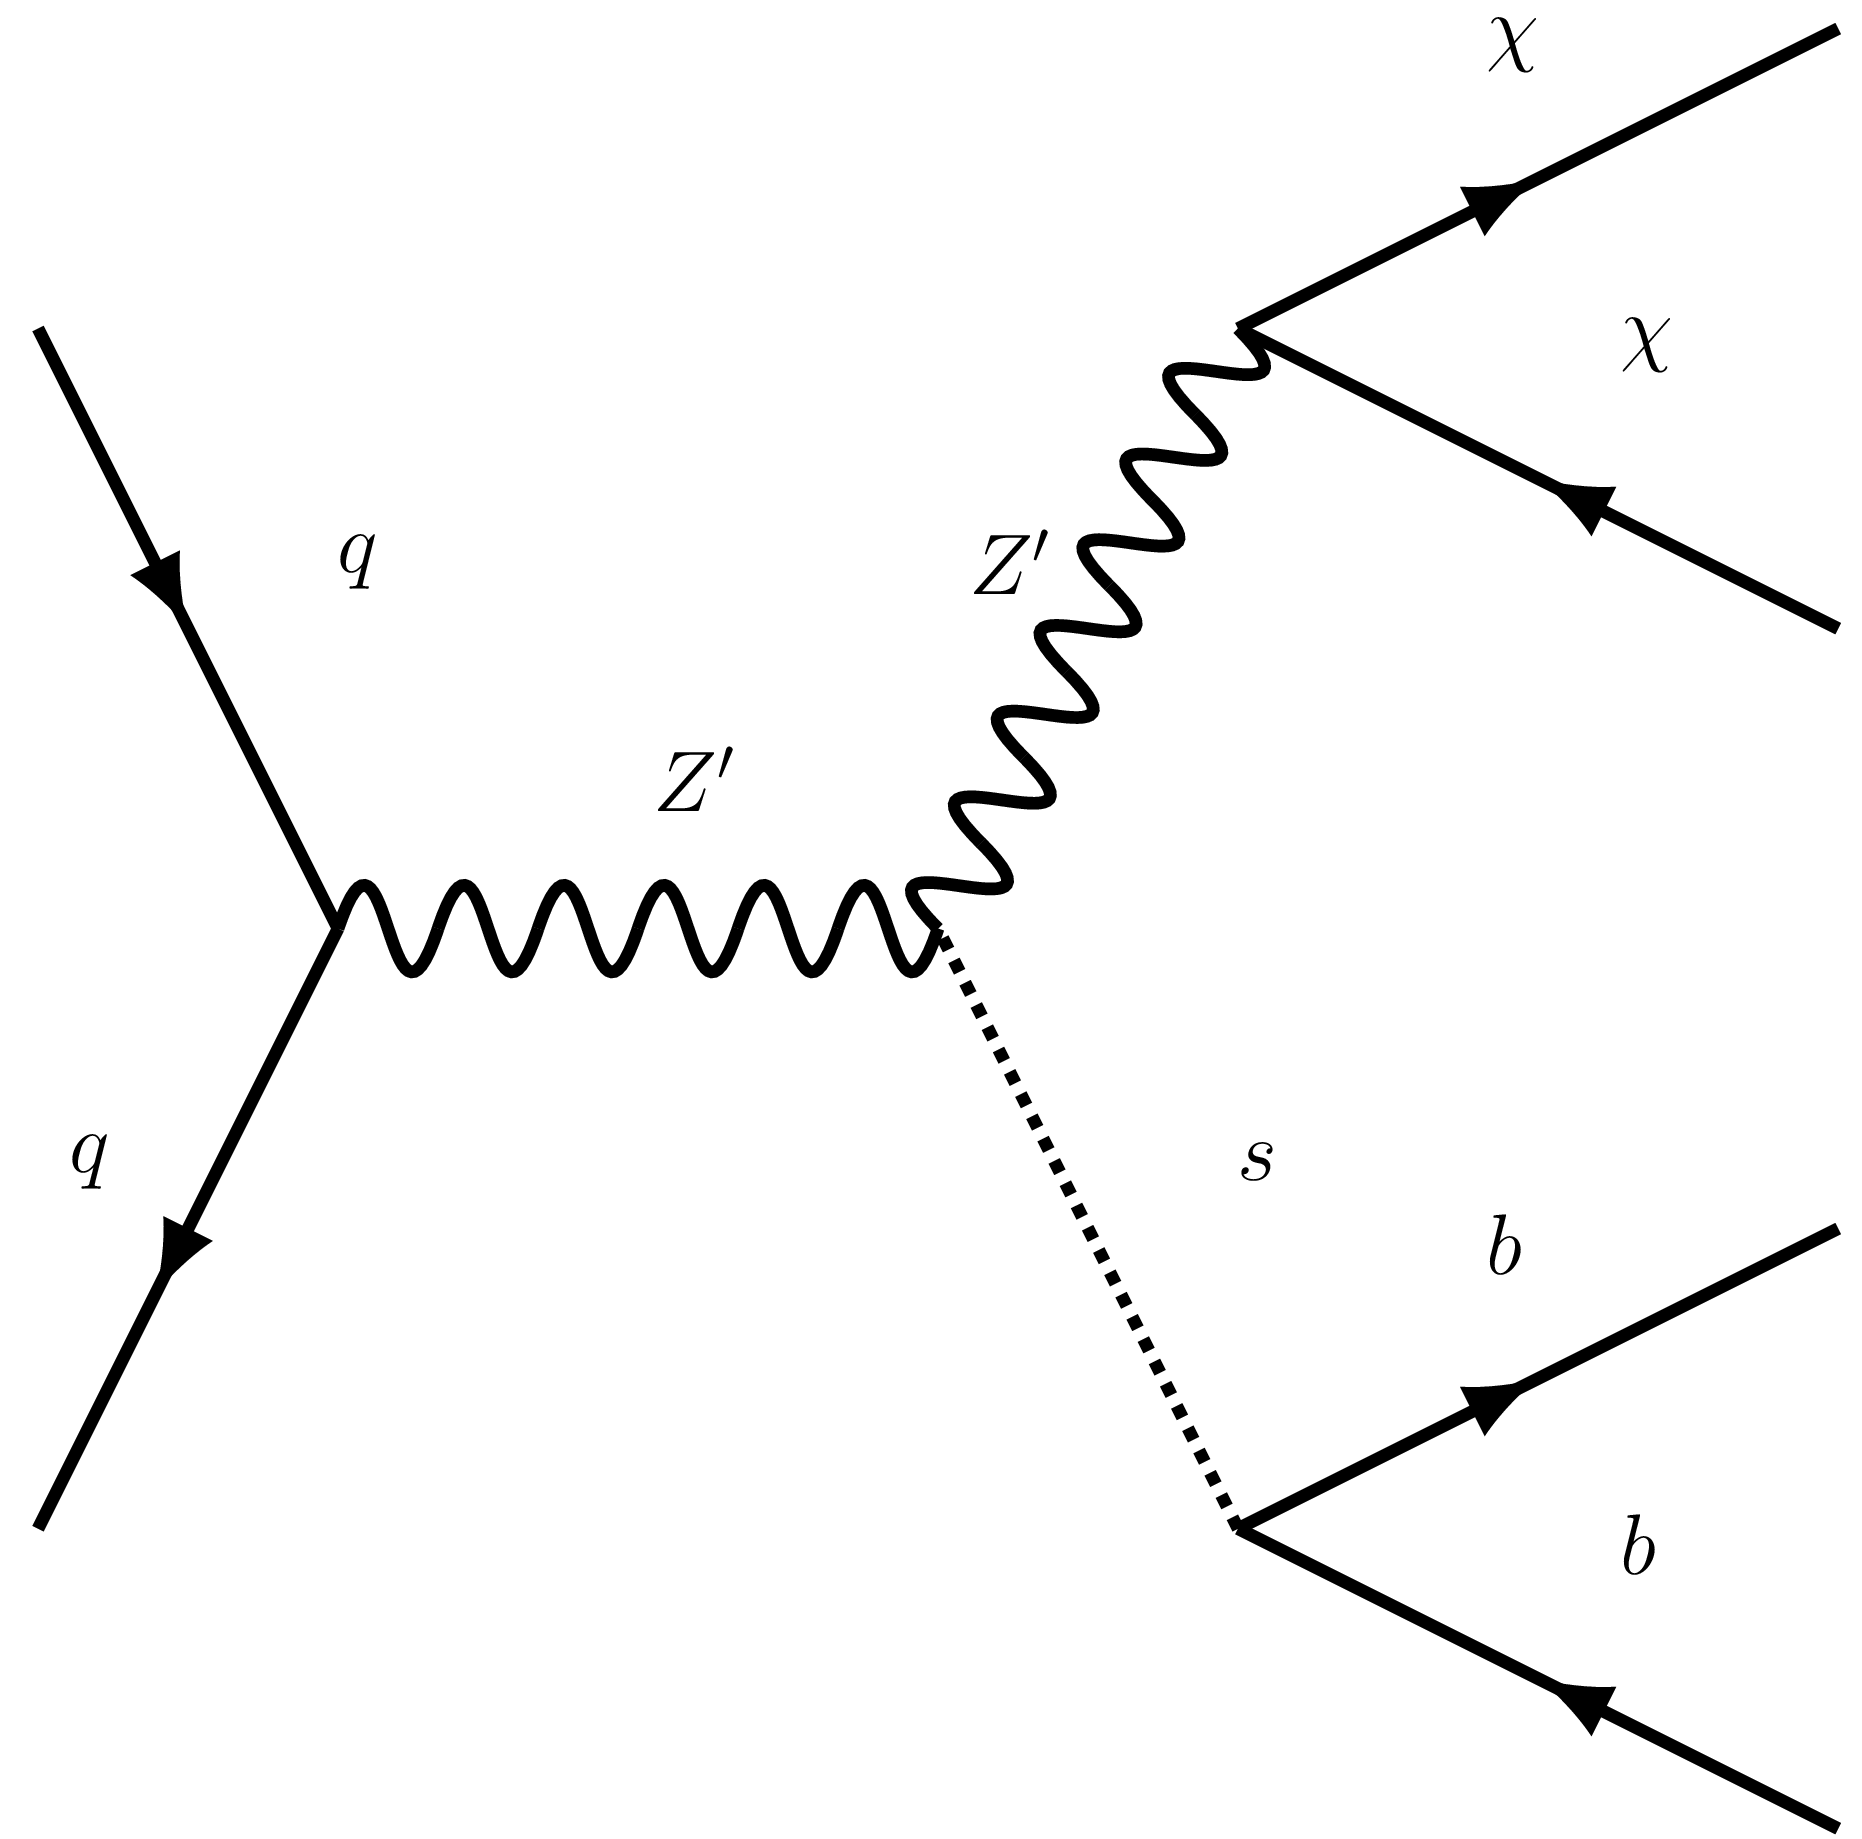
\includegraphics[width=0.5\textwidth]{figures/feyns/mono-hs.pdf}
   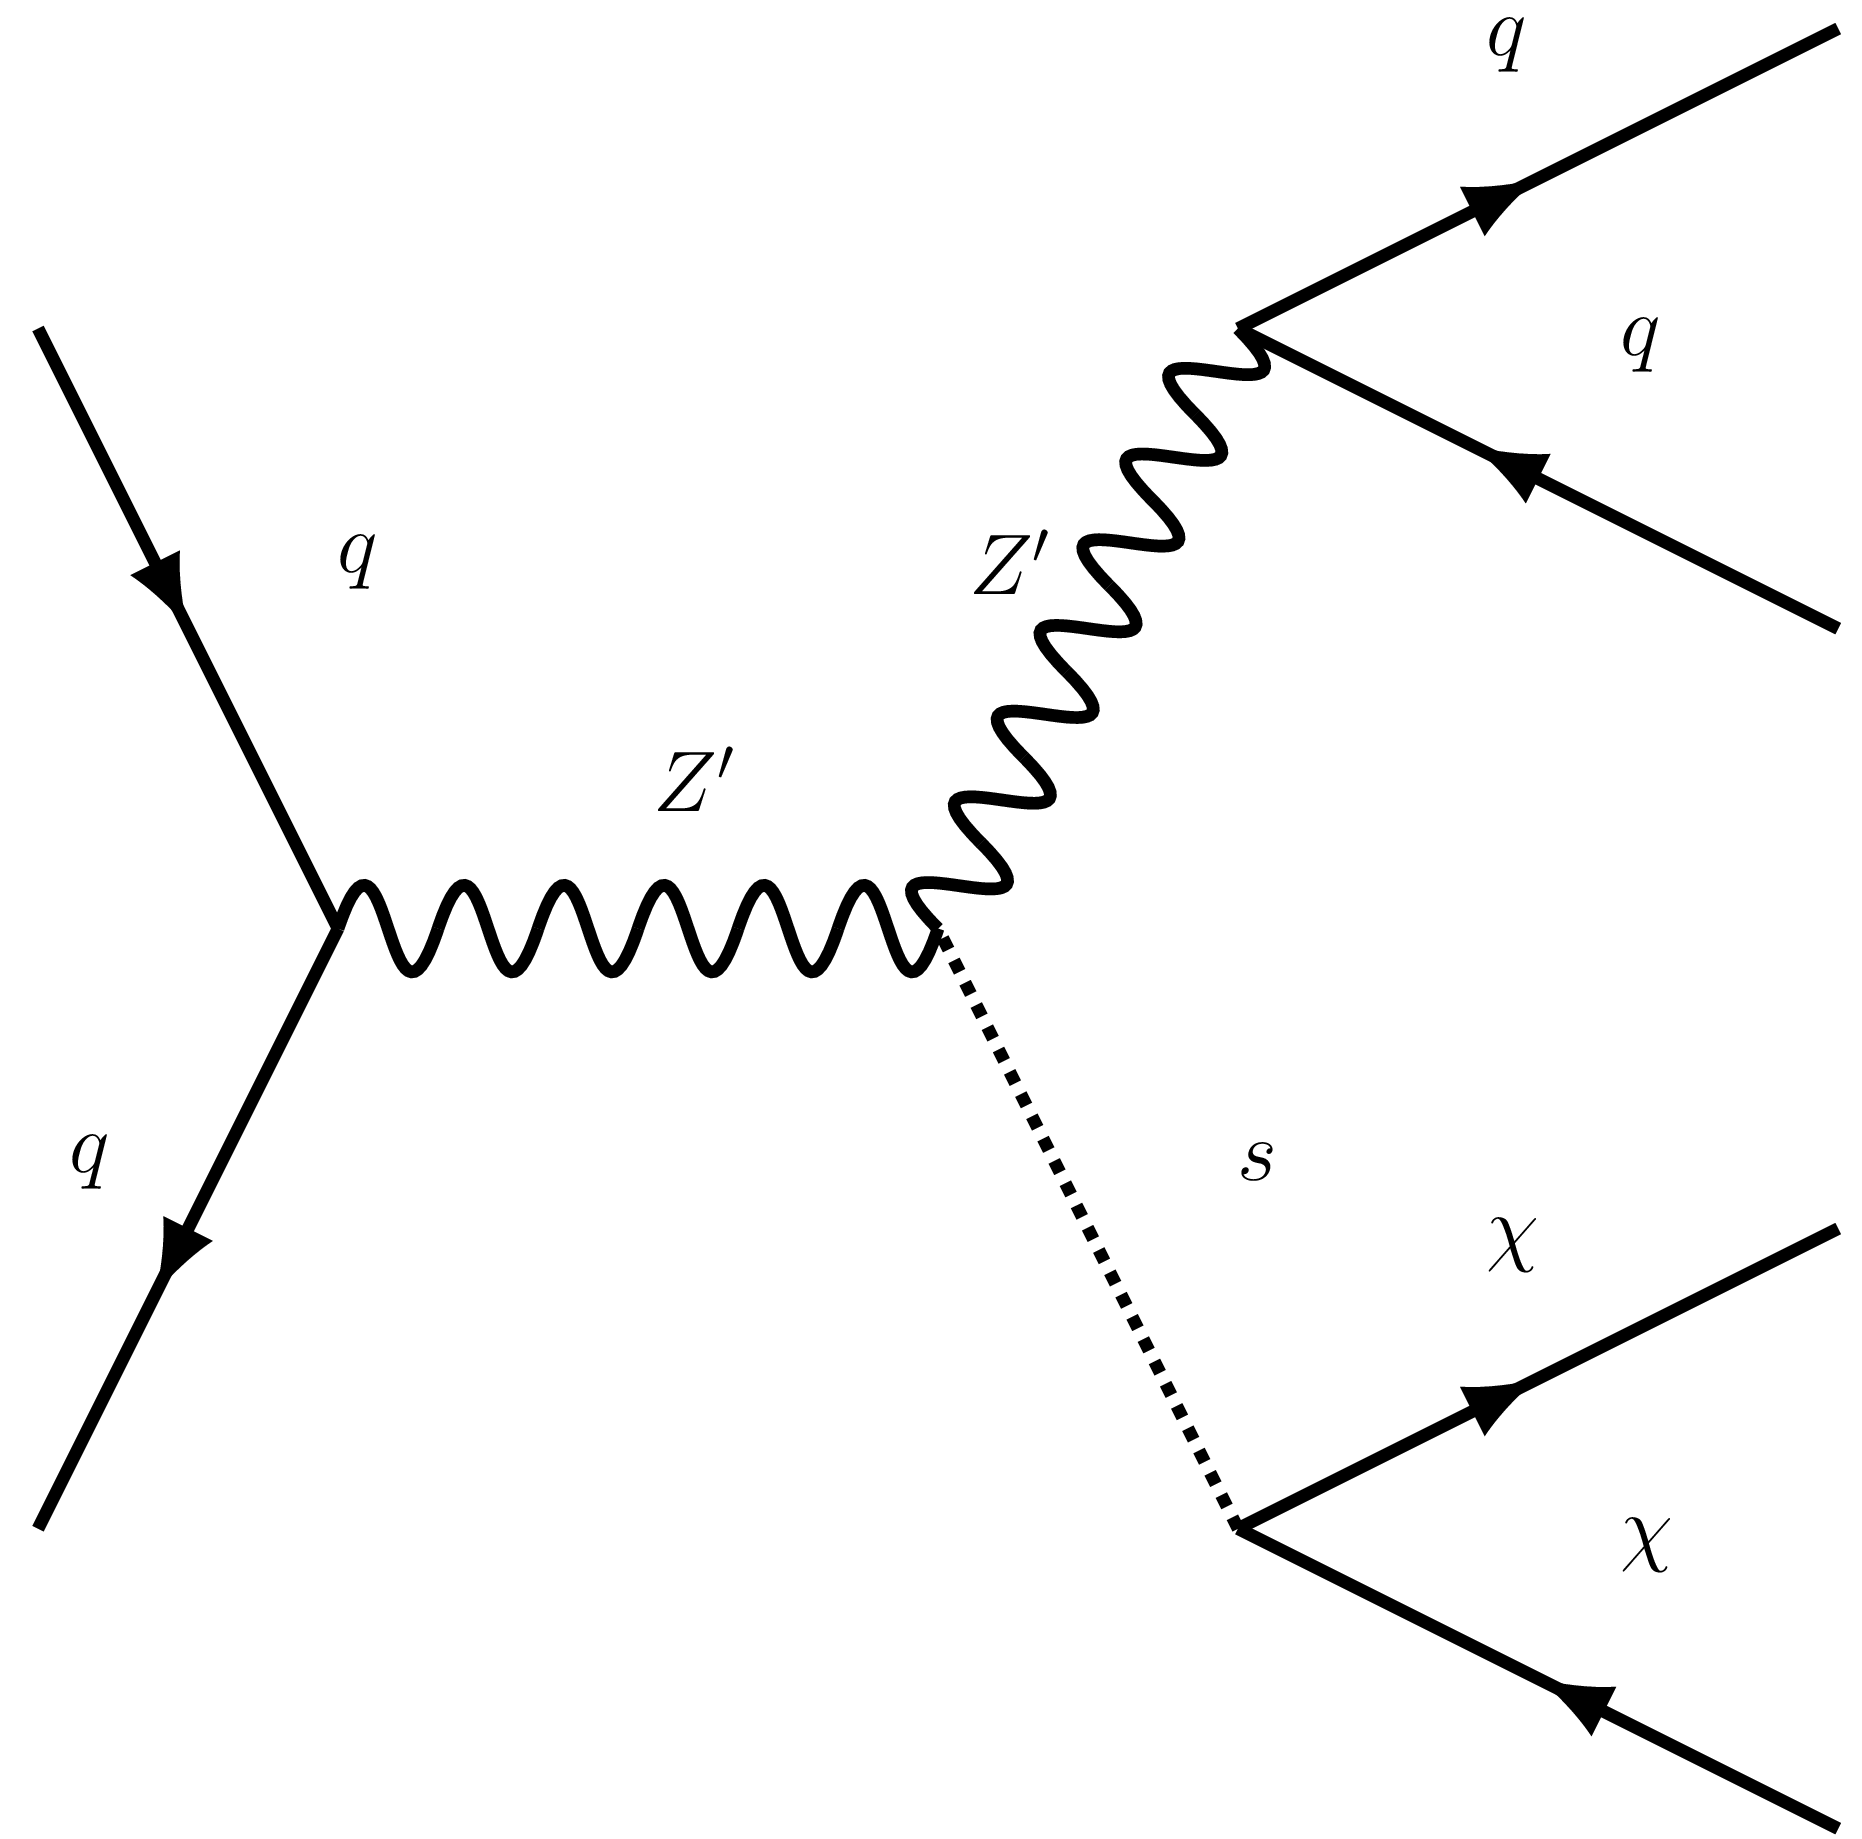
\includegraphics[width=0.5\textwidth]{figures/feyns/mono-Zp.pdf}
   \caption{Left: Feynman diagram of a visible dark Higgs production final state. Right: Feynman diagram of a visible Z' final state. Both proceeded with an off-shell Z' mediator with dark Higgs boson radiated off and eventually decay into SM final state. Both final states give rise to highly boosted jet with \MET signature.}
   \label{fig:feynman}
\end{figure}

We consider a Majorana DM particle $\chi$ that obtains its mass from the vacuum expectation value (vev) $w$ of a new complex Higgs field $S$, which is a singlet under the DM gauge group. The field $S$ carries a charge $q_{S}$ under a new $U(1)^{\prime}$ gauge group, so its vev $w$ breaks the gauge symmetry spontaneously and generates the mass of the corresponding $Z^{\prime}$ gauge boson. The symmetry breaking gives rise to a new physical Higgs boson. Under the dark Higgs model~\cite{Duerr2017}, the DM particle acquires an axial coupling to the $Z^{\prime}$, so that all three particles in the dark sector couple to each other.

We will be interested in the case where the DM particle is not the lightest state in the
dark sector, so that it can annihilate into other dark sector states which subsequently decay
into SM states. Scenarios in which the $Z^{\prime}$ is the lightest particle are typically disfavoured,
because they require the couplings of the dark Higgs boson to be close to the perturbativity
bound~\cite{Bai2015,PhysRevD.92.035007}. We therefore focus on the more natural case that the dark Higgs boson is the
lightest state in the dark sector and the relic density is largely set by the process $\chi\chi\rightarrow ss$.

The two mediators offer three different possibilities in which such a dark sector can
be coupled to the SM: via direct couplings of the $Z^{\prime}$
to SM particles, via mixing of the $Z^{\prime}$ with the neutral gauge bosons of the SM or via mixing between the dark Higgs boson and
the SM Higgs boson. In particular, non-zero mixing between the dark Higgs boson
and the SM Higgs boson ensures that the dark Higgs boson is unstable even if it is the
lightest state in the dark sector and decays into SM states with a negligible lifetime. The
required mixing angle can however be so small that it does not lead to any other observable
effects. For the purpose of this work we assume that the dominant interaction results from
vector couplings  of the $Z^{\prime}$ to quarks, which naturally arise in models of gauged baryon
number. 

There is also an obvious similarity to the spin-1 simplified DM model studied by the
LHC collaborations~\cite{Kahlhoefer2016}, with the one addition that we specify the mechanism
responsible for generating the masses of the DM particle and the $Z^{\prime}$ and for this purpose
introduce a dark Higgs. Since the couplings of the dark Higgs boson are fully specified
by the other parameters in the model, the only new parameter is the dark Higgs mass $m_{s}$. In order to be consistent with the benchmark introduced from ATLAS-CMS DM forum~\cite{Abercrombie:2015wmb}, we adopt $g_{q}$ = 0.25 and $g_{\chi}$ = 1.

With the requirement on the choice of coupling which allows to make contact with existing DM searches at the LHC, the observed DM relic abundance is only reproduced for certain combinations of the masses of the particles in the dark sector.

%\subsection{ \cPZpr-Baryonic model}
%A Z' vector boson is a well-motivated feature of many new physics scenarios. 
%The Z'-motivated DM models are more interesting since the corresponding U(1)' 
%gauge symmetry ensures DM stability. The model is an extension of the SM and 
%assumes that the baryon number (B) is gauged, with the Z' being the gauge 
%boson of U(1)$_{B}$. The consistency of theory requires the existence of new 
%stable baryonic state that are neutral under SM gauge symmetry. This new 
%particle is an excellent DM candidate. If the DM particle carries a baryon 
%number $B_{\chi}$, the Z'-quark-DM part of the Lagrangian for models with 
%fermionic dark matter is 
%\begin{equation}
%{\cal L} = g_q \bar{q}\gamma^{\mu}q\cPZpr_{\mu}+g_{\chi}\bar{\chi}\gamma^{\mu}\chi\cPZpr_{\mu}
%\end{equation}
%To generate the Z' mass, a ``baryonic Higgs'' scalar is introduced to 
%spontaneously break the U(1)$_B$ symmetry. Analogous to the SM, there remains 
%a physical baryonic Higgs particle, $h_{B}$, with a coupling of h$_{B}$Z'Z' 
%and vacuum expectation value of v$_{B}$. 
%The \cPZpr\ and SM Higgs boson h interact with a coupling strength of 
%$g_{h\cPZpr\cPZpr} = m_{\cPZpr}^{2} \sin \theta/v_{B}$, where $\theta$ is the h-h$_{B}$ 
%mixing angle. This allows for mono-Higgs final states at the LHC as shown in 
%Fig.~\ref{fig:feynman}. In the search for this model, values for $g_q$ and $g_\chi$ are chosen to be 0.25 and 1, respectively. The ratio $g_{h\cPZpr\cPZpr}/M_{\mathrm{Z}'}$ is chosen to be unity. All these parameter choices follow the recommendations from~\cite{Abercrombie:2015wmb}.  



%\begin{figure}[htbp]
%   \centering
%   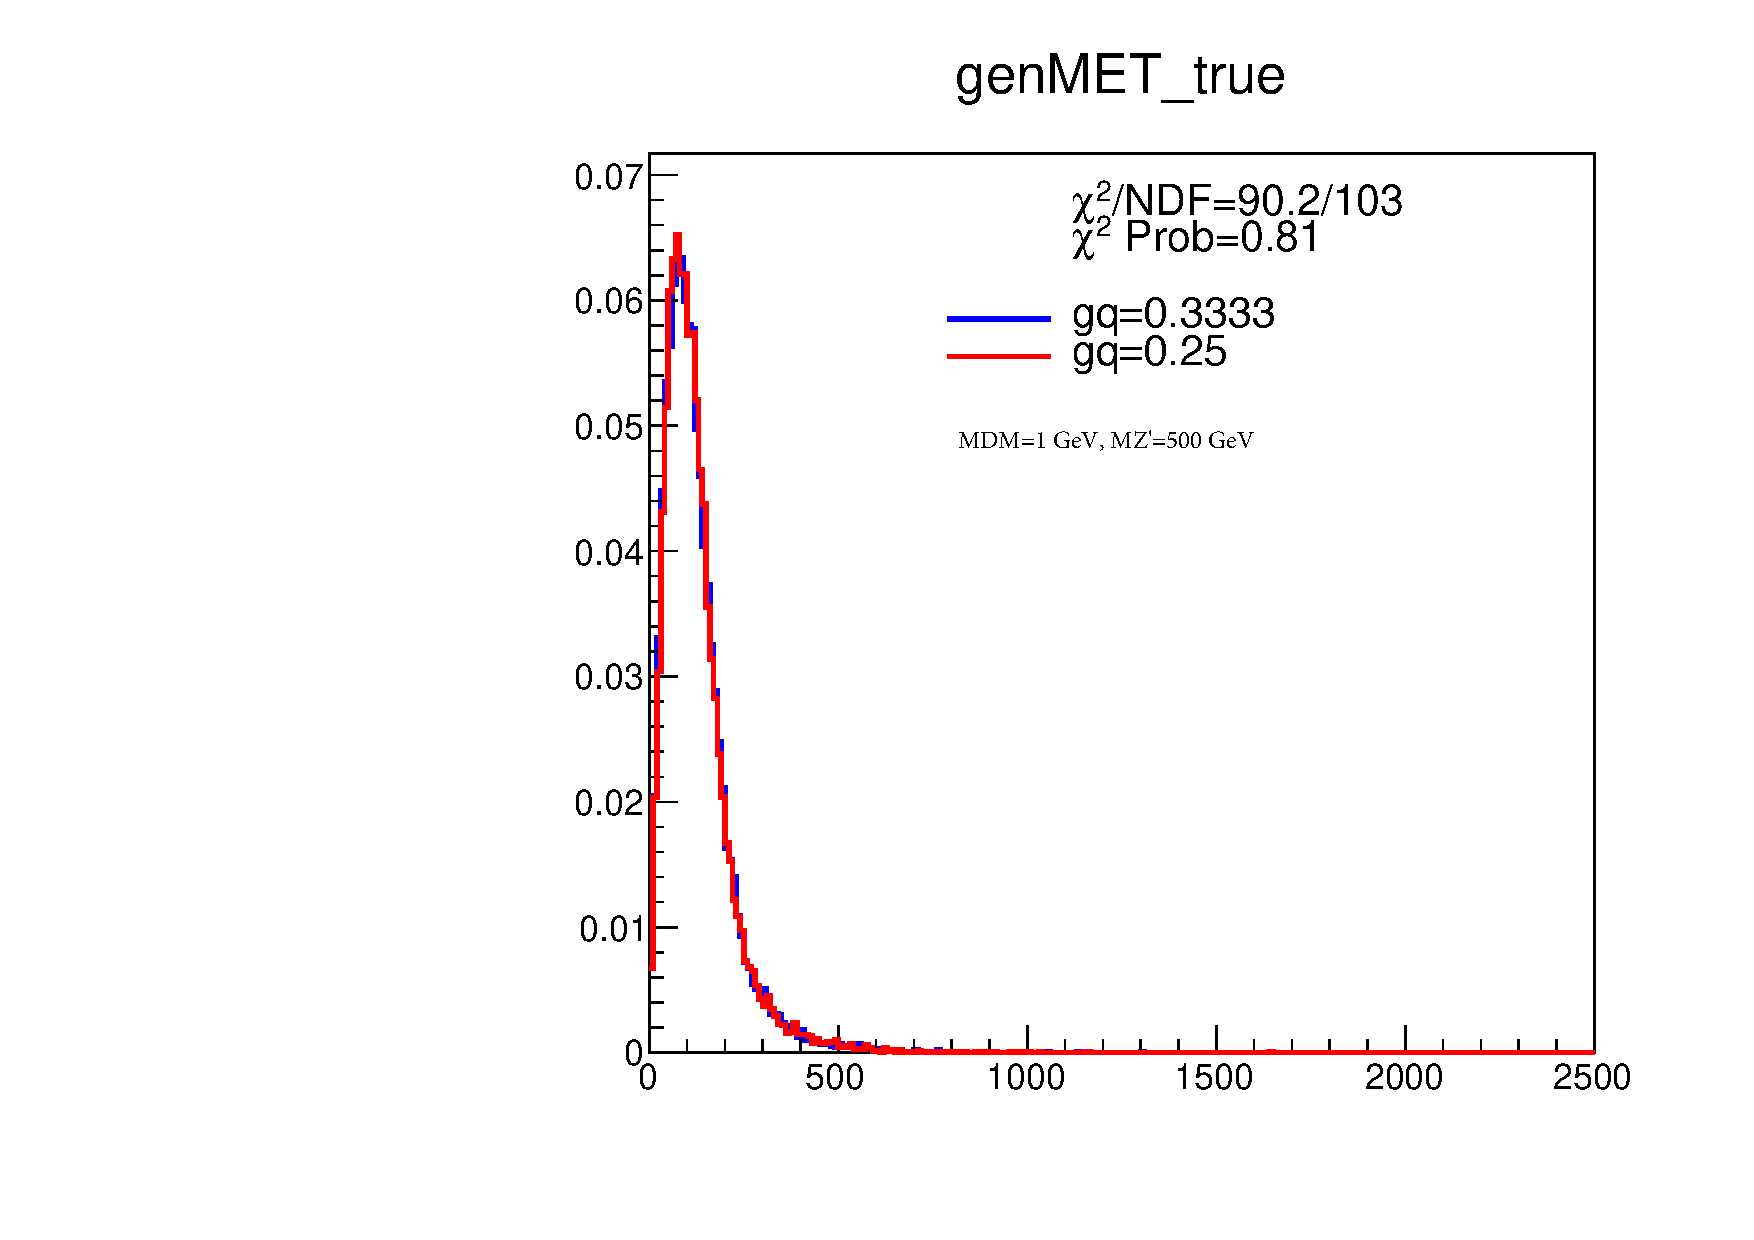
\includegraphics[width=0.7\textwidth]{figures/models/gq0p3333_ZpBaryonic_MSC500_MDM1_gq0p25_ZpBaryonic_MSC500_MDM1.pdf}
%   \caption{Comparison of the generator-level \MET\ distributions predicted 
%by the \cPZpr-Baryonic model (after parton shower by \PYTHIA) for $g_q=0.25$ and $g_q=0.3333$. The mass of 
%the dark matter particle is set to 1~\GeV and the mass of the mediator 
%\cPZpr\ is set to 500~\GeV, respectively. Samples for this model have been generated with $g_q=0.3333$; however, as the kinematics does not change, we% use them to interpret the results under the assumption $g_q=0.25$ by appropriately rescaling the cross section.}
%   \label{fig:METZpBgq}
%\end{figure}

%\begin{figure}[htbp]
%   \centering
%   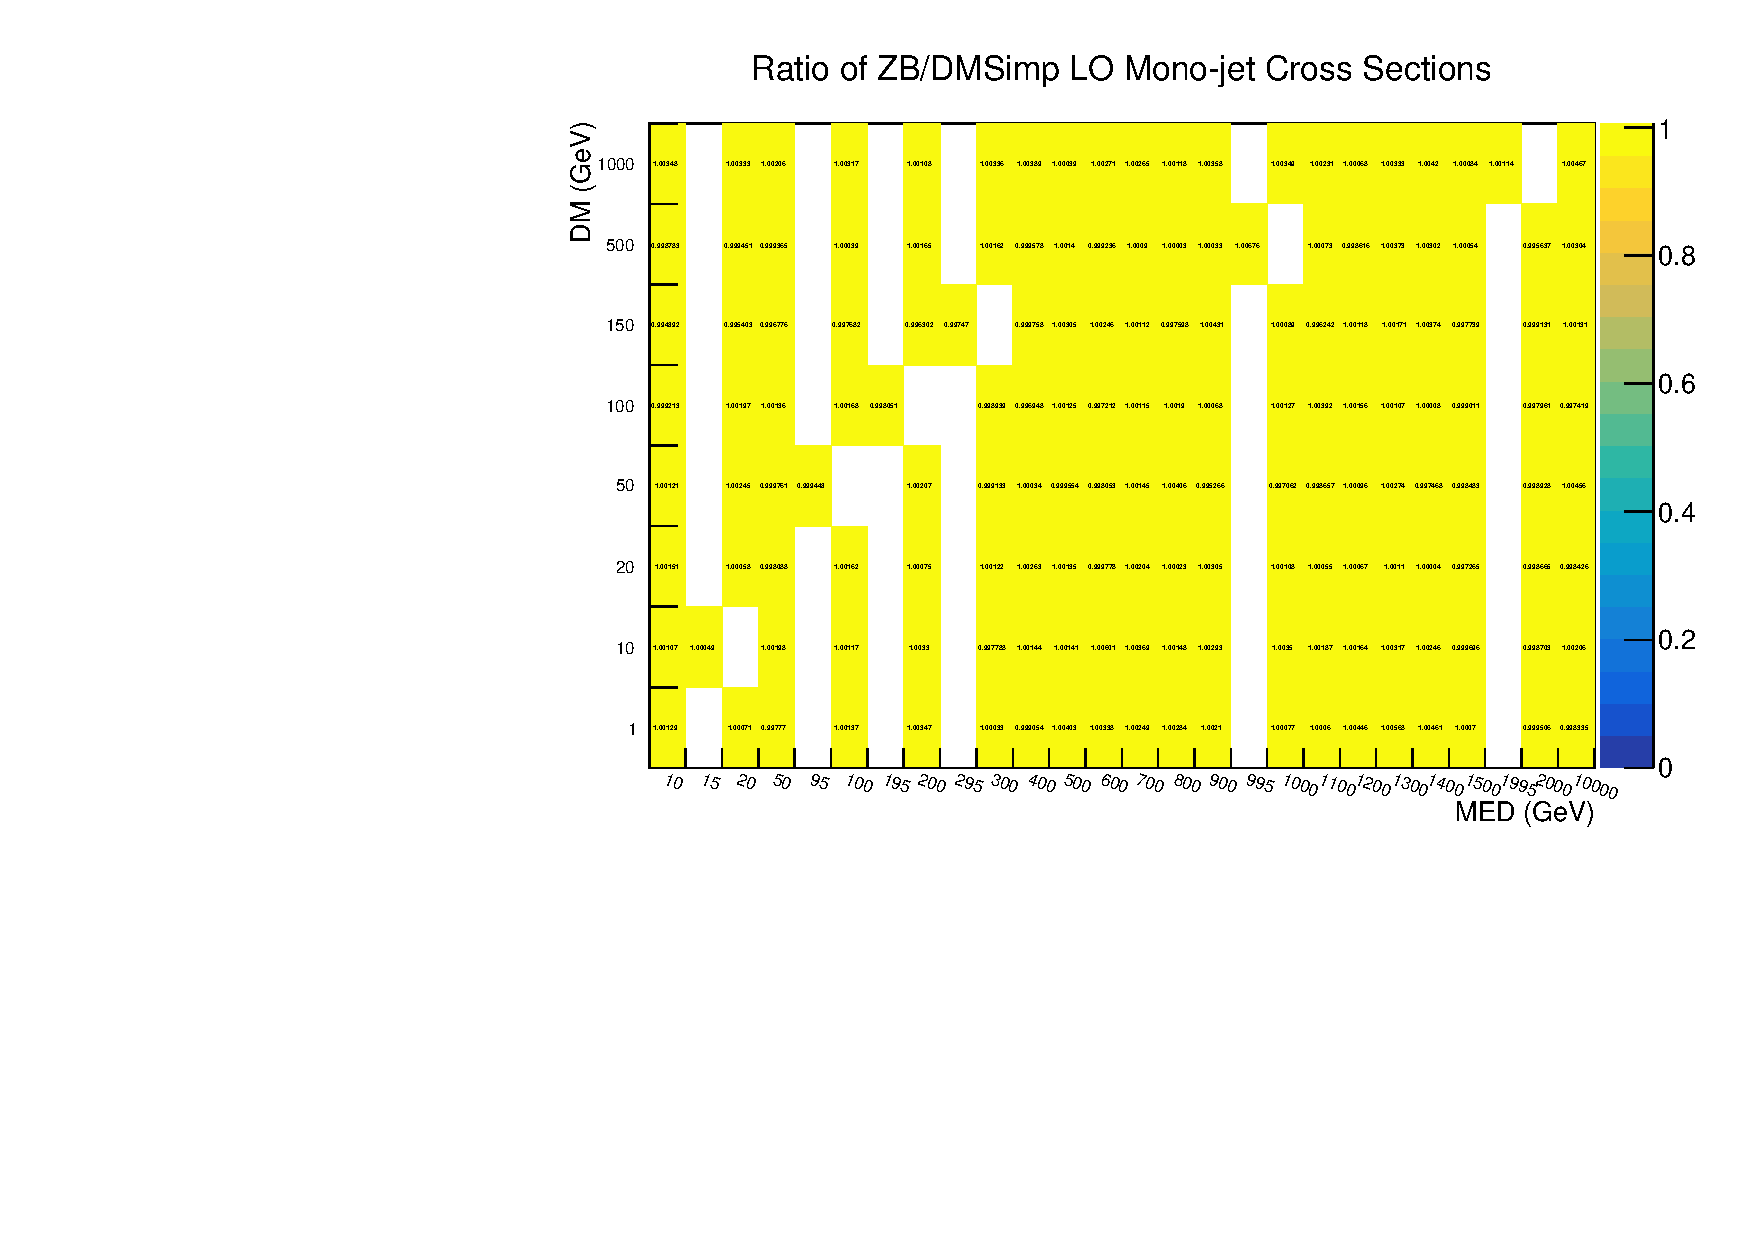
\includegraphics[width=0.45\textwidth]{figures/models/xsec_ZBToDMSimp.pdf}
%   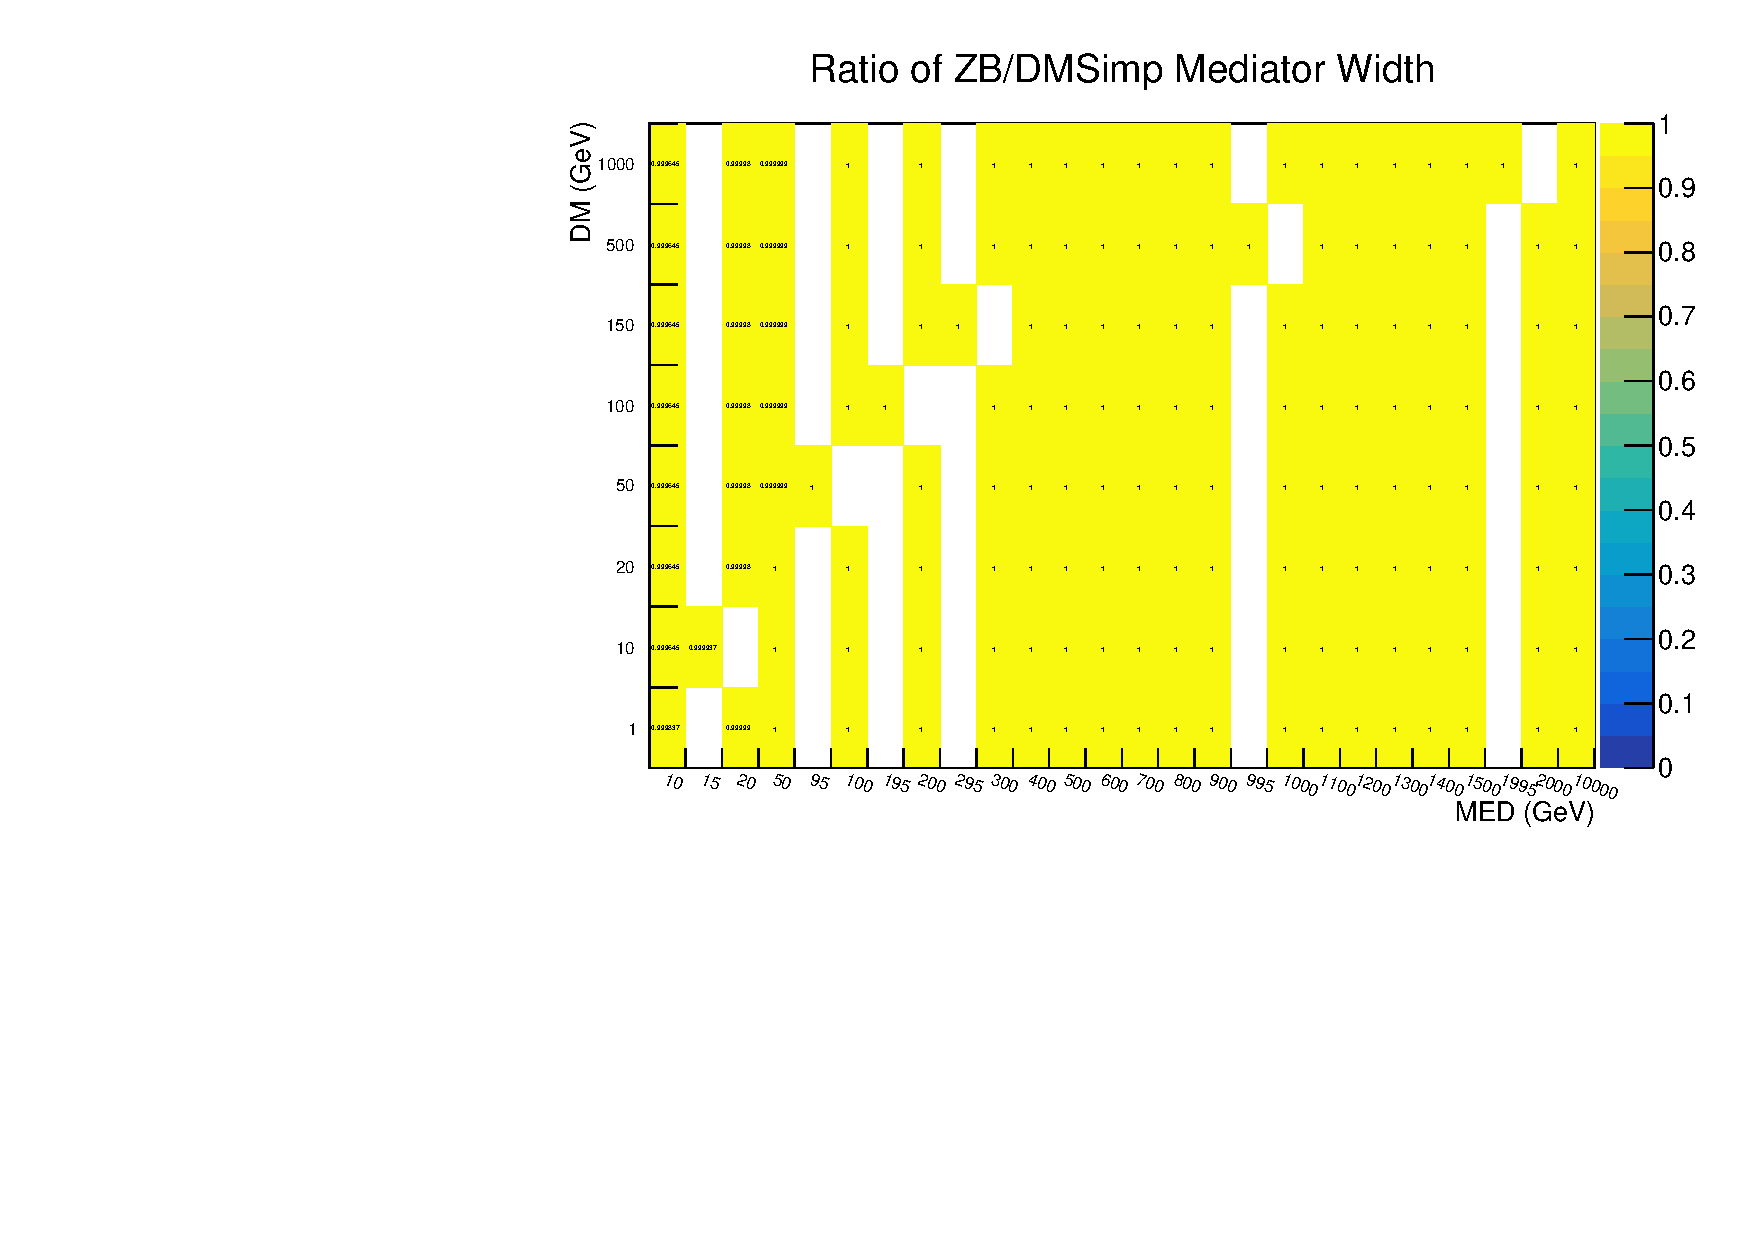
\includegraphics[width=0.45\textwidth]{figures/models/width_ZBToDMSimp.pdf}
%   \caption{Ratios of the leading-order mono-jet cross sections (left) 
%and $\Gamma_{\cPZpr}$ (right) predicted by the \cPZpr-Baryonic model 
%relative to that 
%predicted by {\sc DMSimp-spin1}. The ratios are consistent with unity.
%}
%   \label{fig:ZBXsWidth}
%\end{figure}



%%%%%%%%%%%%%%%%%%%%%%%%%%%%%%%%
%The \MET distributions for many different mass combinations for both models investigated are shown in Fig.~\ref{fig:puppimet_models}. 

%\begin{figure}[htbp]
%   \centering
%   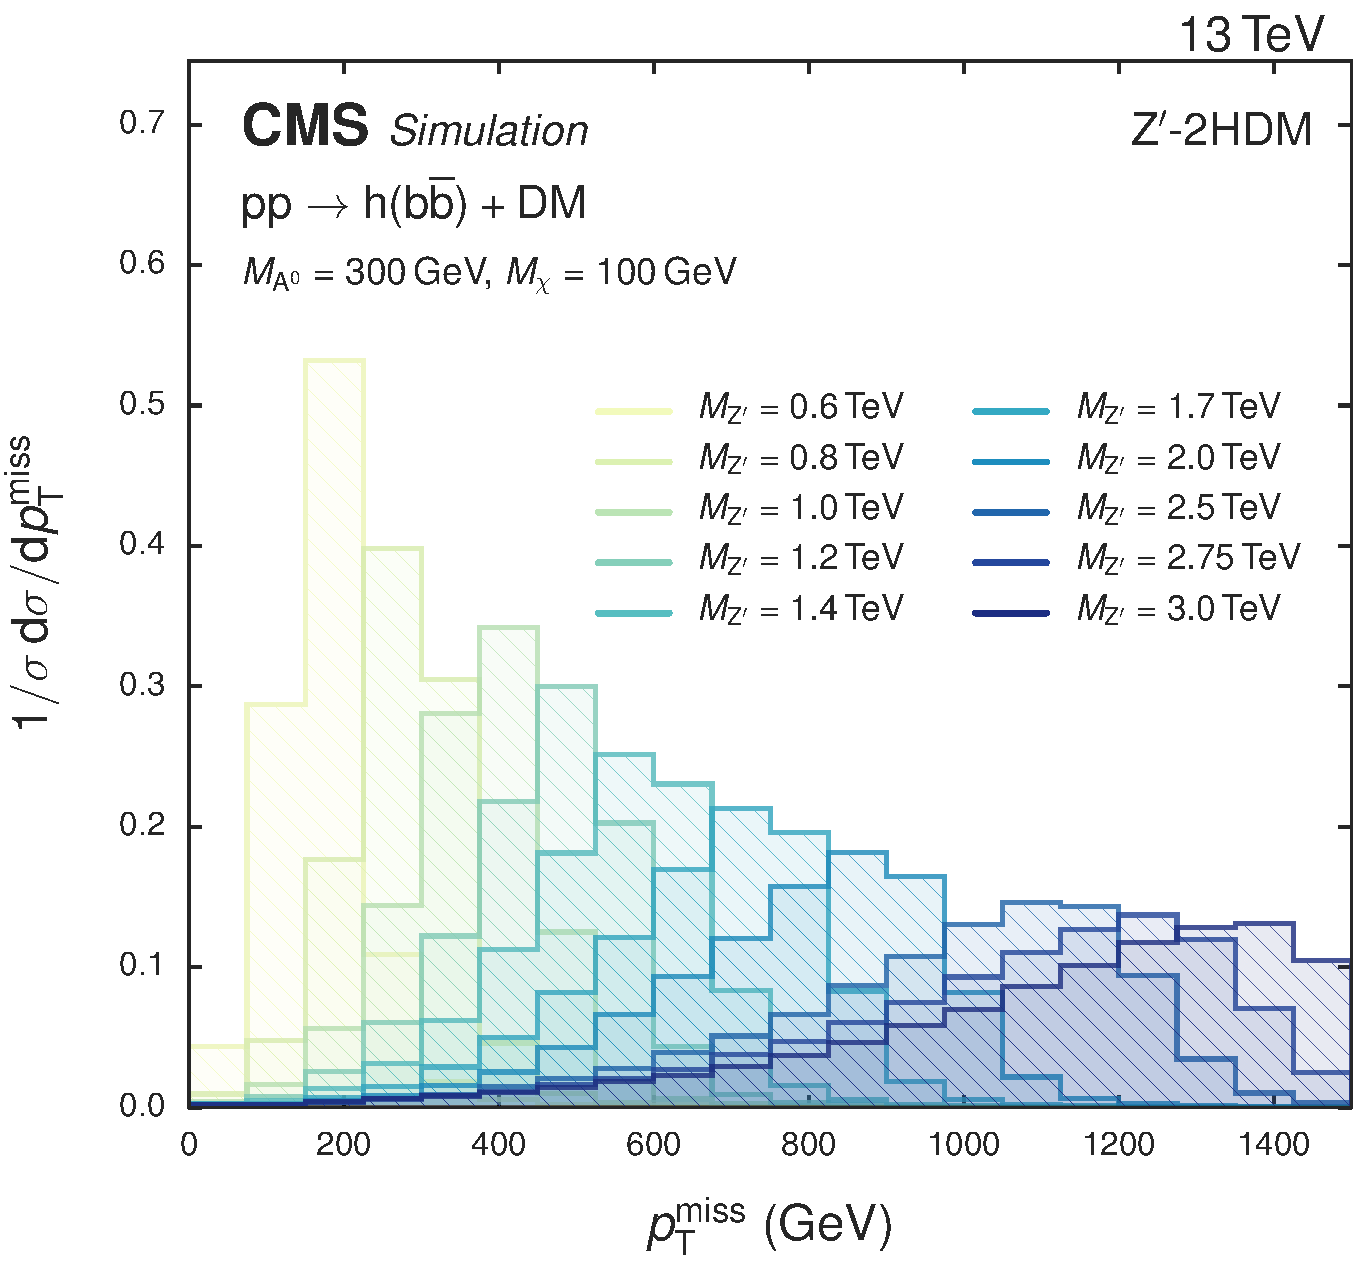
\includegraphics[width=0.43\textwidth]{figures/models/puppimet_signals_2hdm.pdf}
%   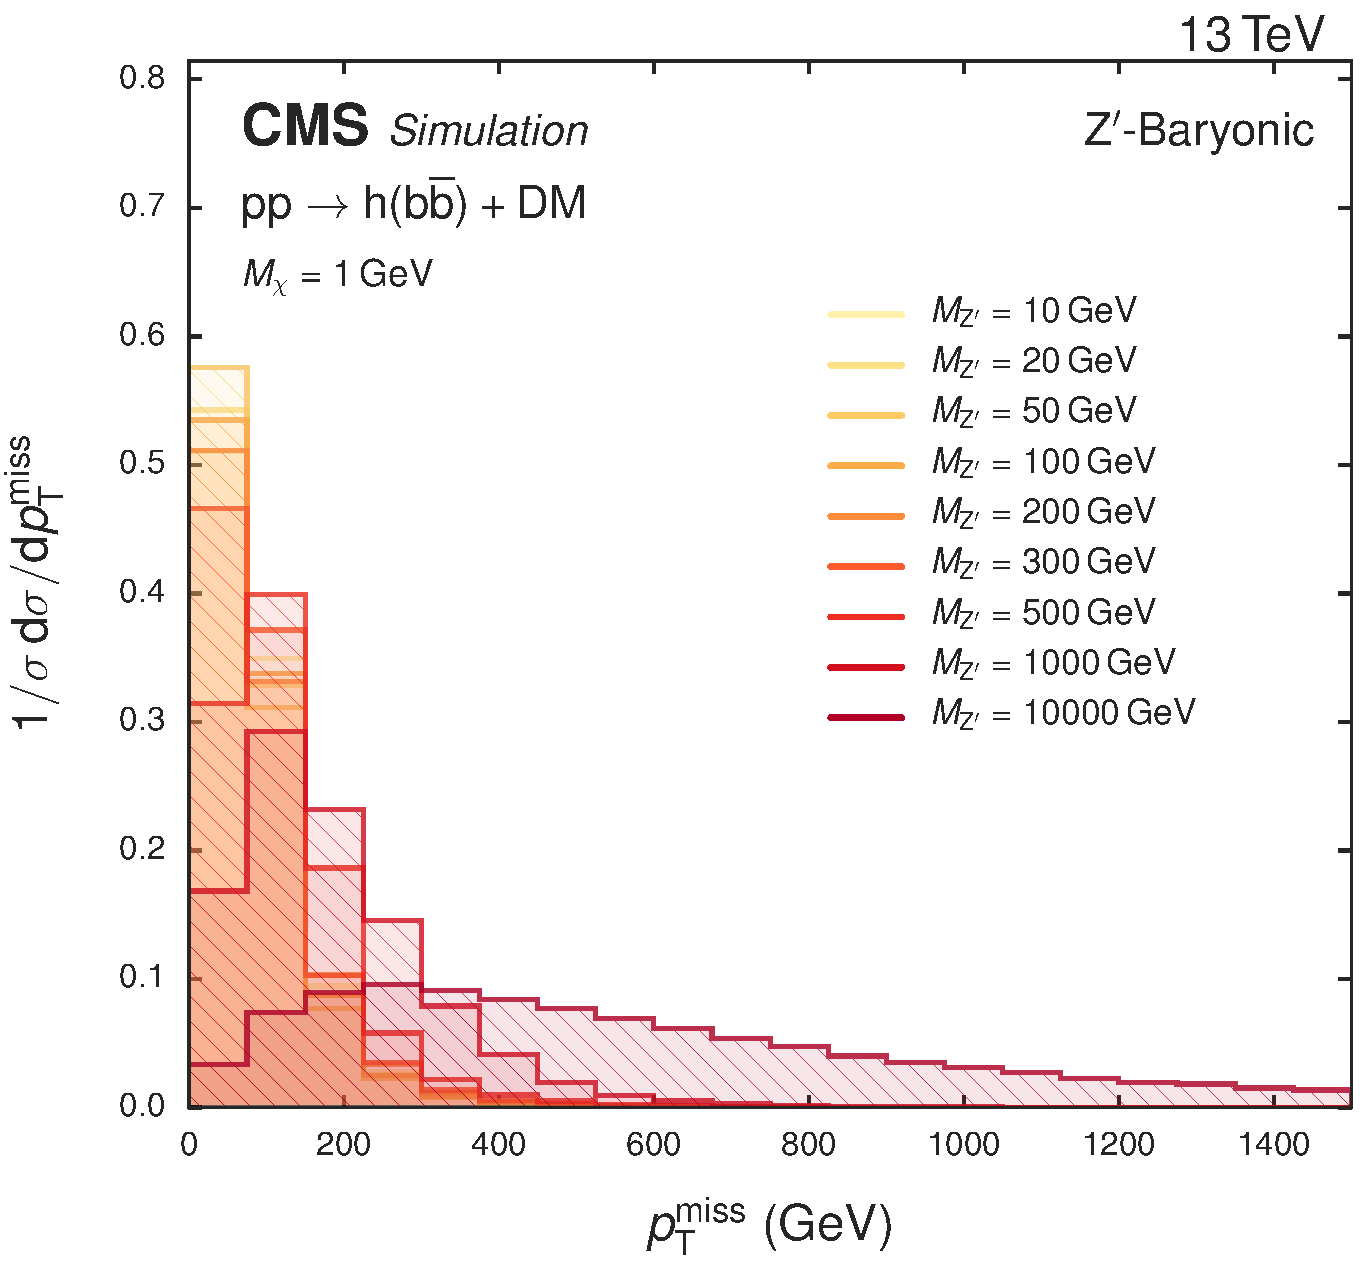
\includegraphics[width=0.43\textwidth]{figures/models/puppimet_signals_barzp.pdf}\\
%   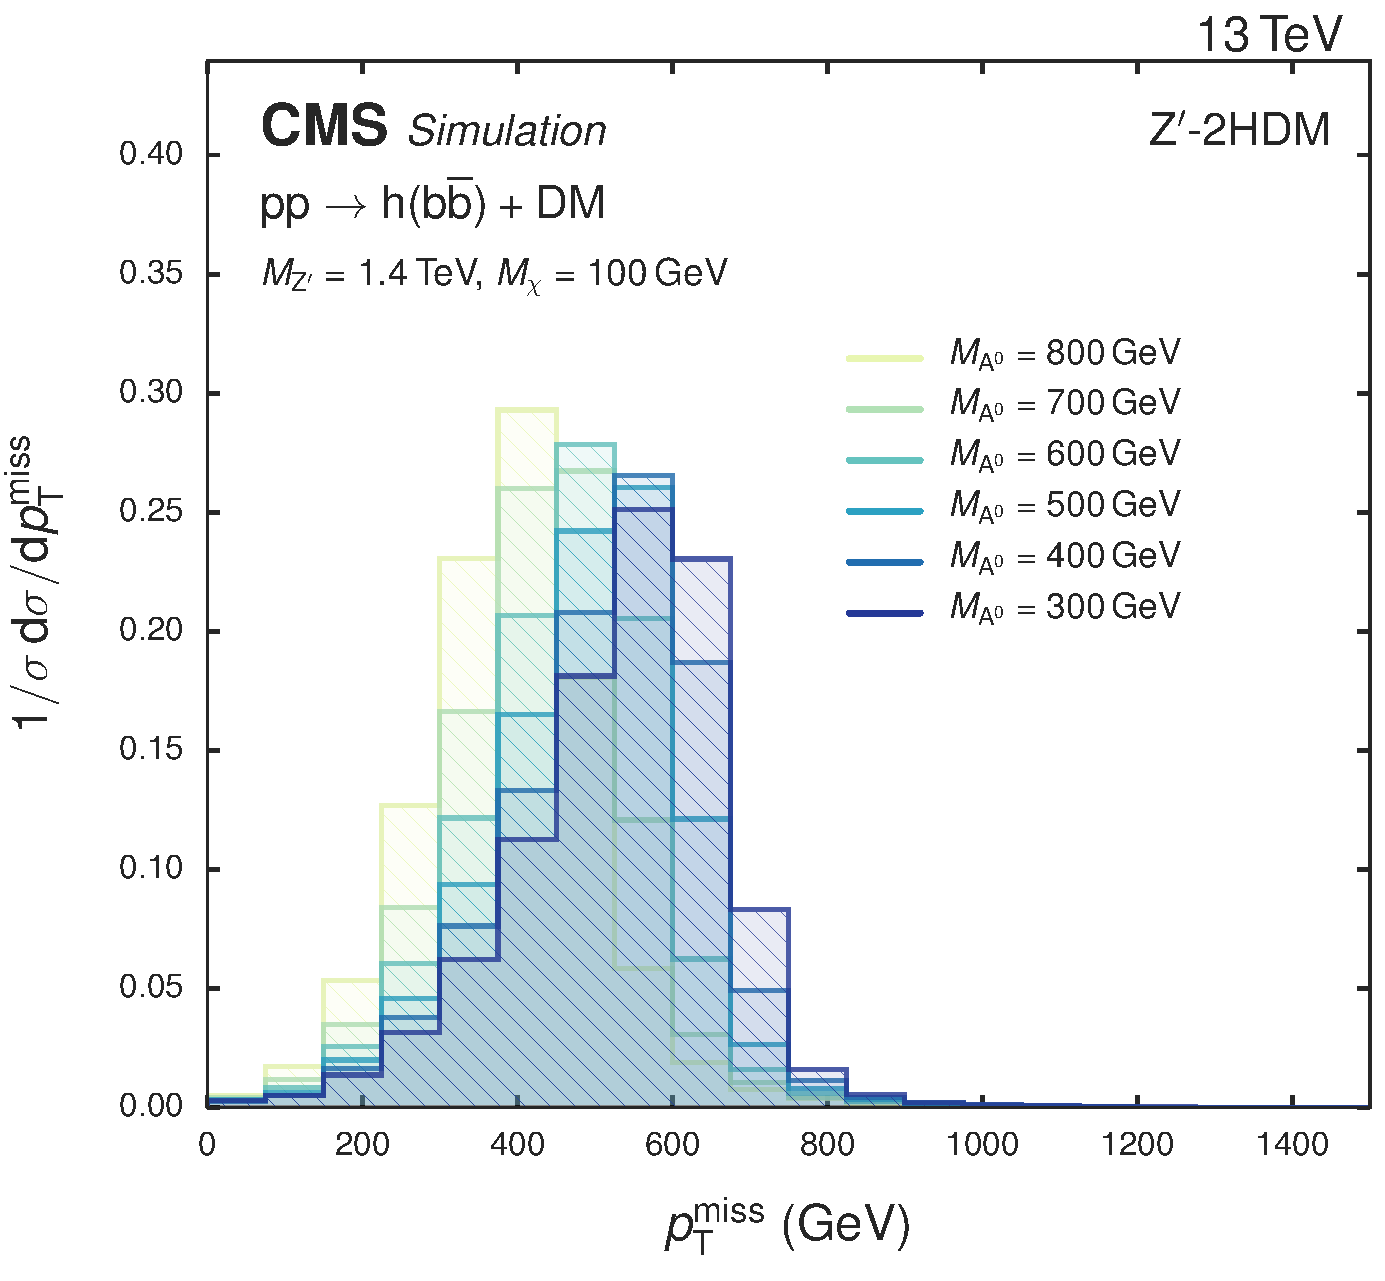
\includegraphics[width=0.43\textwidth]{figures/models/puppimet_signals_2hdm-300.pdf}
%   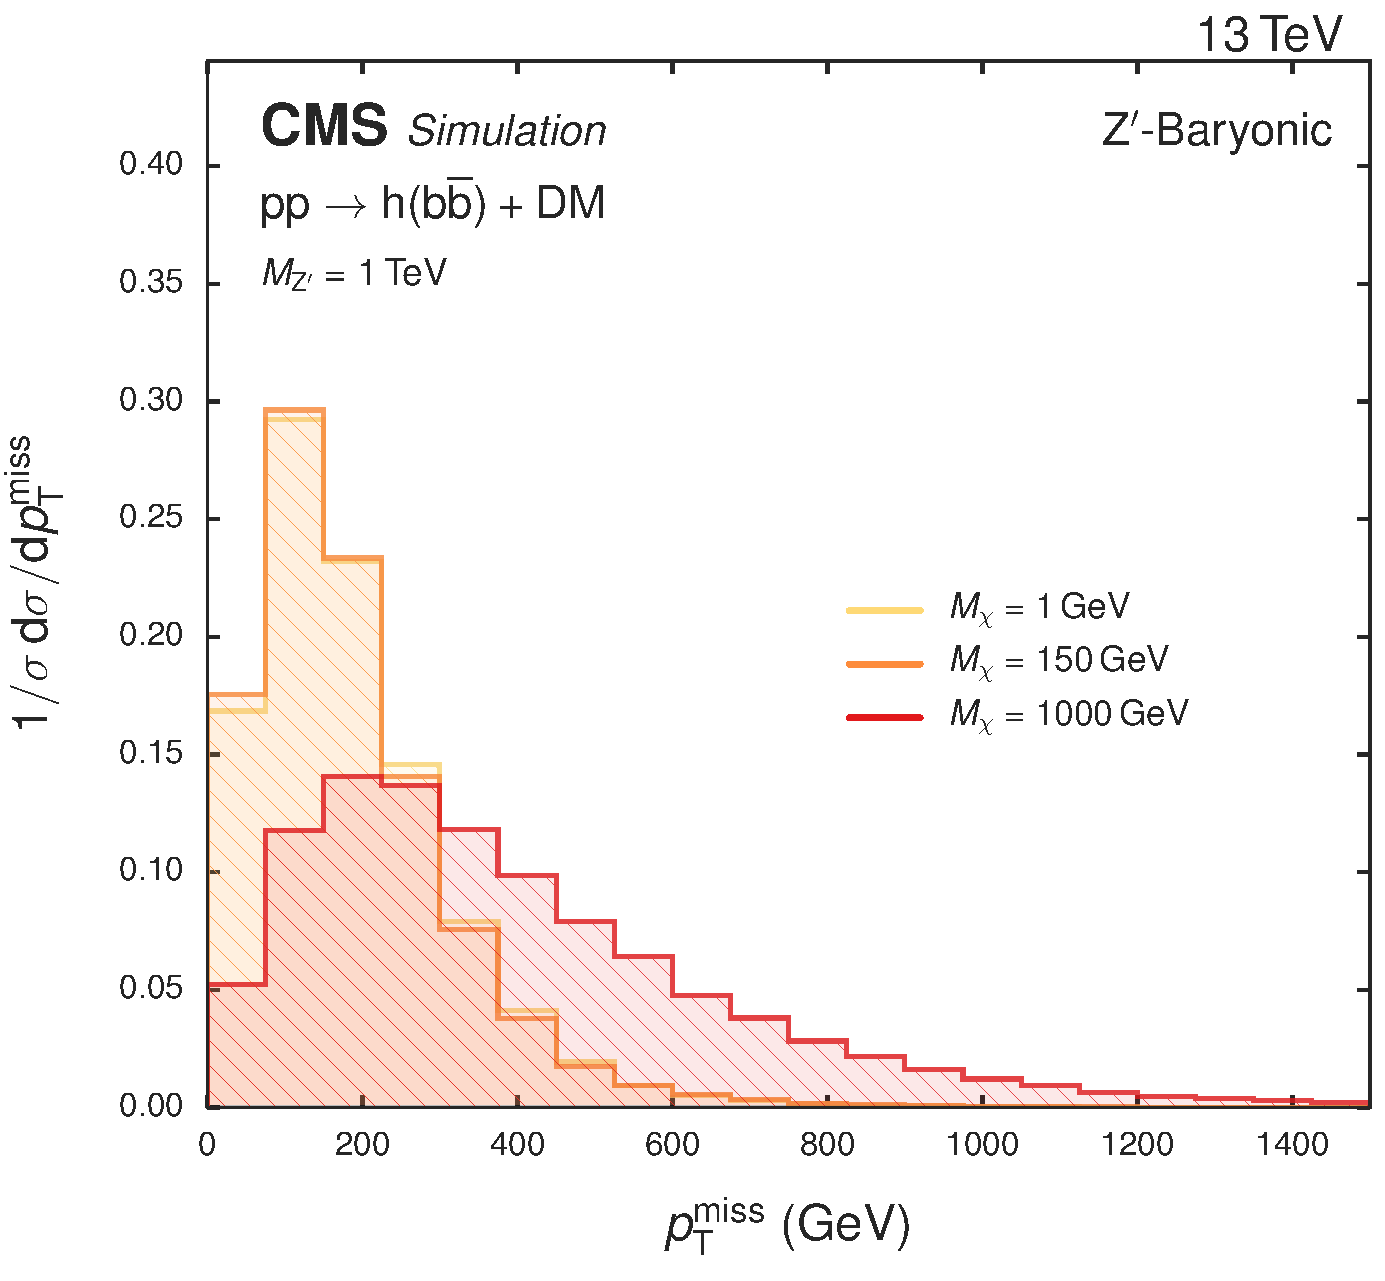
\includegraphics[width=0.43\textwidth]{figures/models/puppimet_signals_barzp-1000.pdf}\\
%   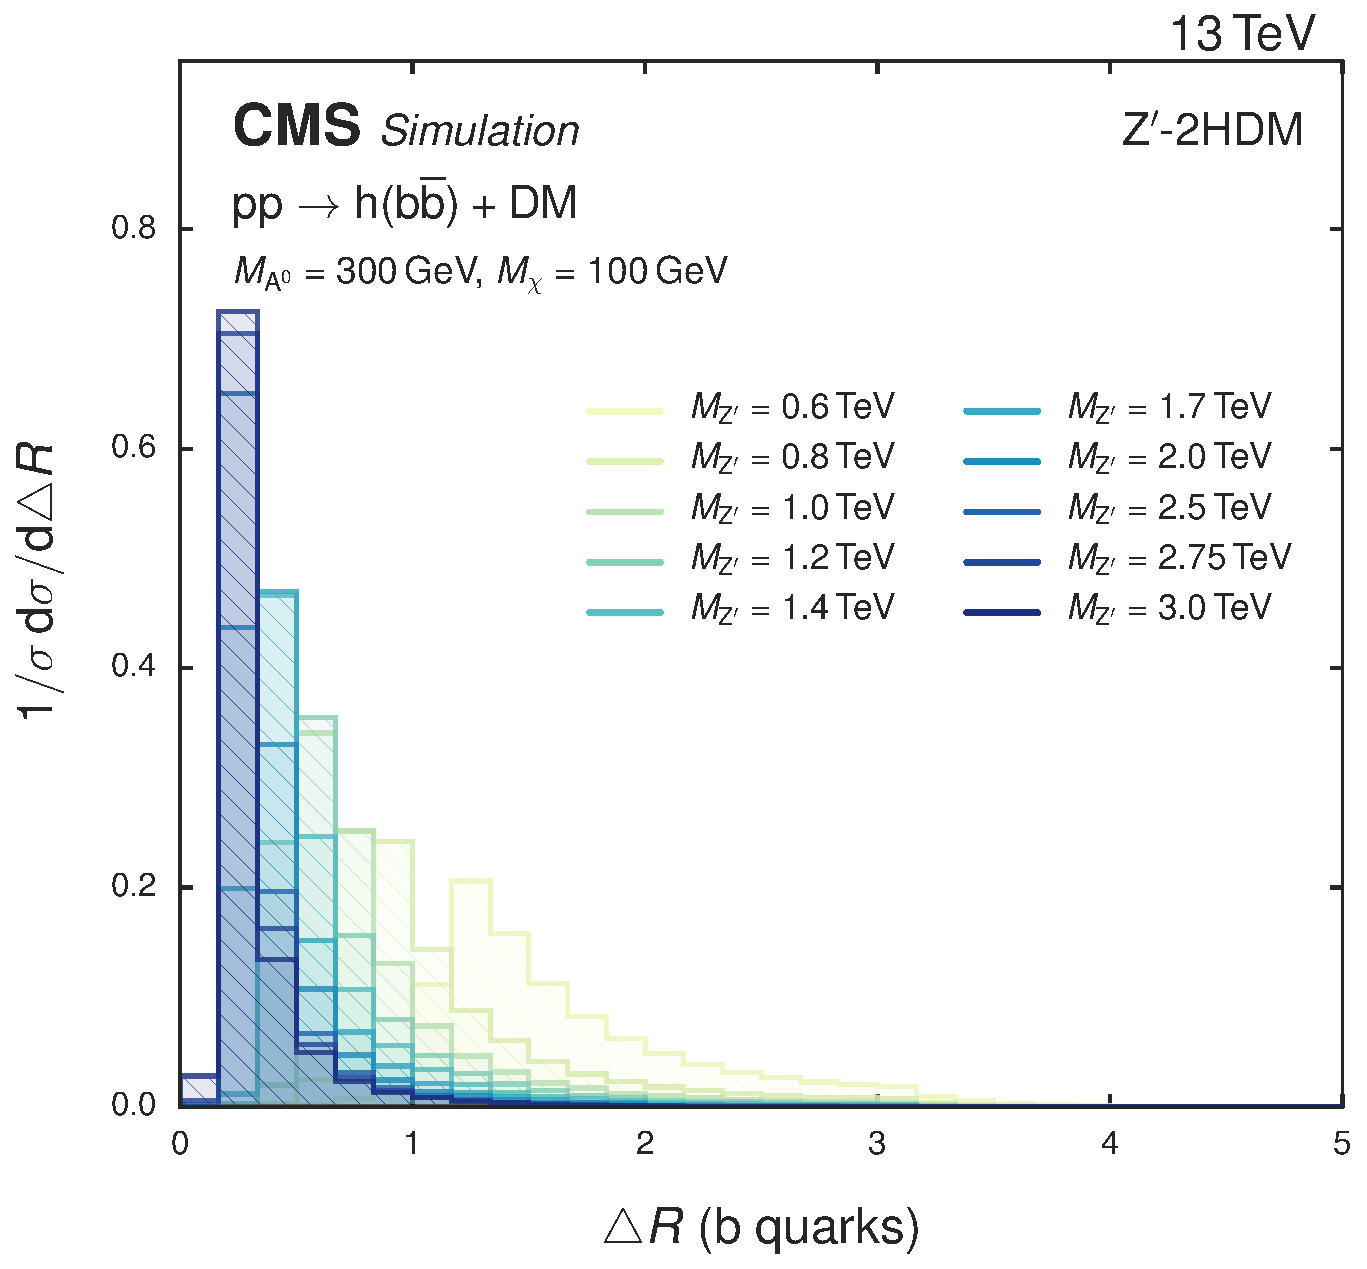
\includegraphics[width=0.43\textwidth]{figures/models/bbdR_signals_2hdm.pdf}
%   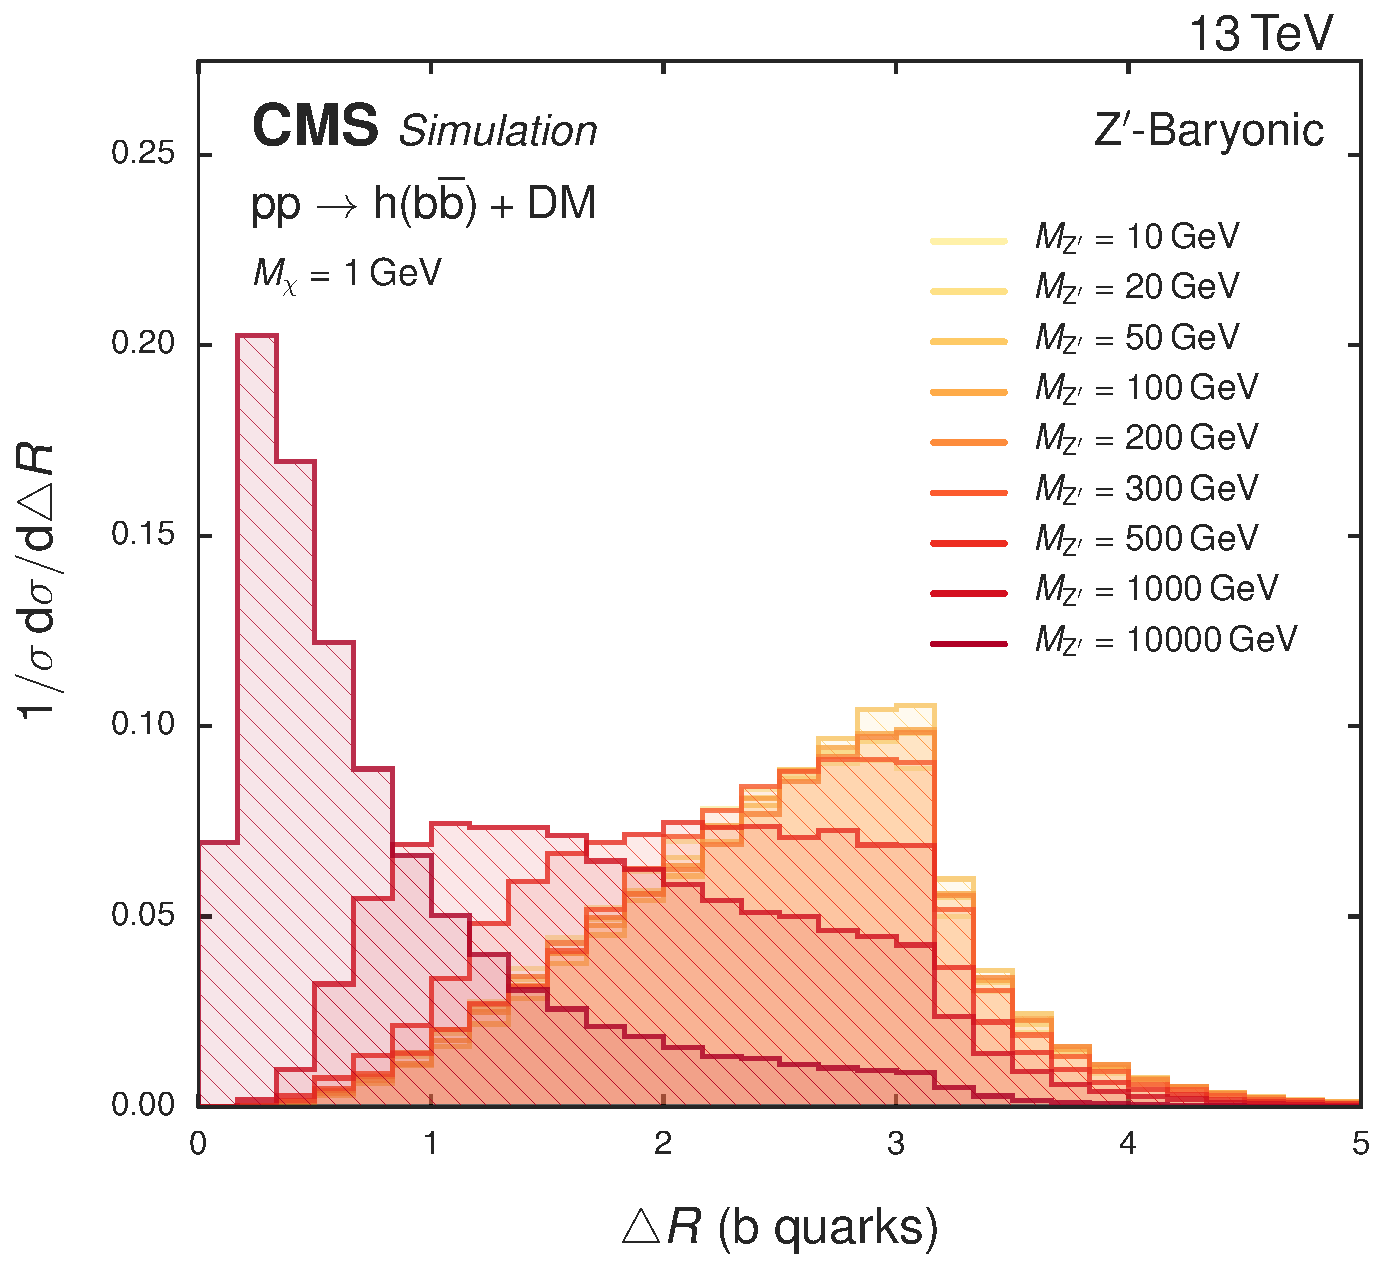
\includegraphics[width=0.43\textwidth]{figures/models/bbdR_signals_barzp.pdf}\\
%   \caption{\ptmiss distributions  for different $M_{\text{Z'}}$ for the Z'-2HDM (upper left) and for the Z'-Baryonic model (upper right); \ptmiss distributions for different $M_{A^0}$ in the Z'-2HDM (middle left) and for different $M_\chi$ (middle right). Lower row: distance between the two b quarks coming from the Higgs boson decay.}
%   \label{fig:puppimet_models}
%\end{figure}


%A direct comparison of the \MET~spectra for the \cPZpr-2HDM and the Baryonic $Z'$ model for similar $M_{\text{Z'}}$ are shown in Fig.~\ref{fig:puppimet_signals}.

%\begin{figure}
%   \centering
%   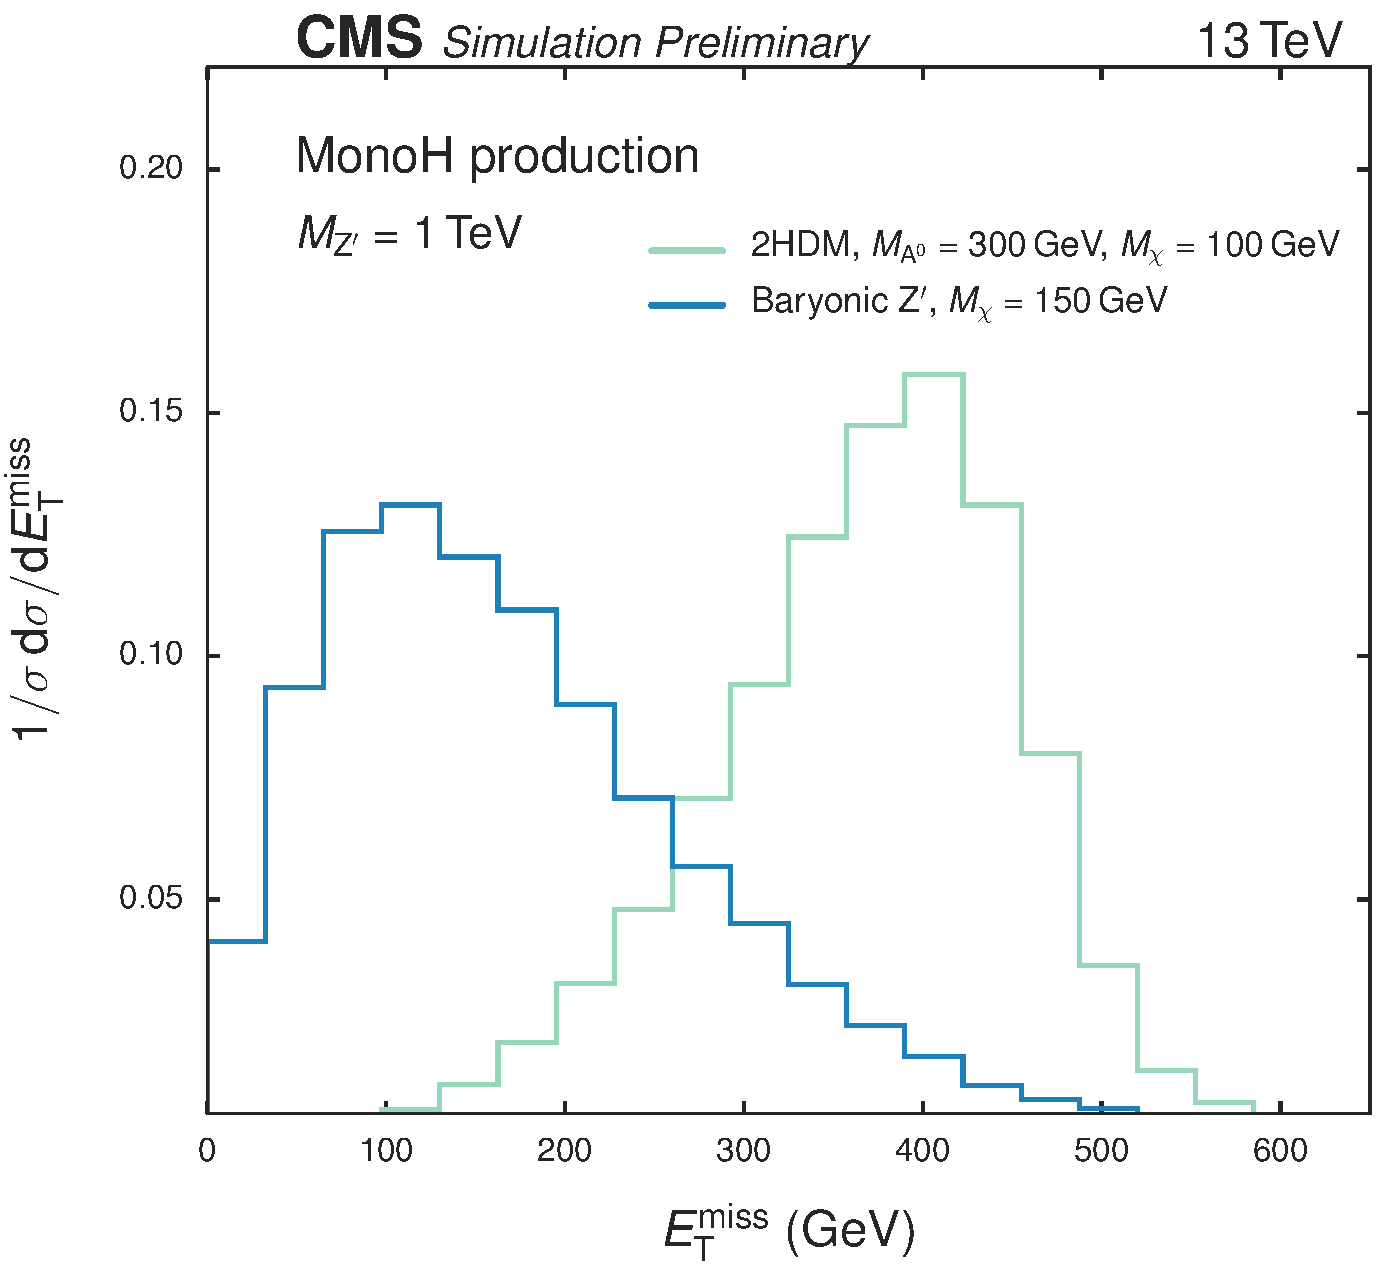
\includegraphics[width=0.6\textwidth]{figures/puppimet_signals.pdf}
%   \caption{\ETslash~spectra for the signal models investigated. The Baryonic $Z'$ model has a significantly softer spectrum.}
%   \label{fig:puppimet_signals}
%\end{figure}


\section{Datasets}\label{sec:datasets}
\subsection{Data and Triggers}

This analysis uses certified events from the Run 2016B-H datasets corresponding to $35.9~\text{fb}^{-1}$. 
It uses control regions defined by muons, and electrons, so the MET and SingleElectron primary datasets are used. 
The MET dataset includes muon pass-through triggers, which allow us to select events with high $\MET$ or high muon recoil. 
A list of all triggers is given in Table~\ref{tab:trigs}. 

\begin{table}[h]
\scriptsize
    \centering
    \begin{tabular}{l|c|c}
\hline
\hline %--------------------------------------------------------------------------------------------------------------------------                
HLT path                                         & L1 seed                   & Primary dataset \\
\hline %--------------------------------------------------------------------------------------------------------------------------                
\verb| HLT_PFMET170_*                          | & \begin{tabular}{c@{}c@{}} \verb| L1_ETM70 or L1_ETM100      | \end{tabular}                                                     & MET \\
\hline
\verb| HLT_PFMETNoMu[X]_PFMHTNoMu[X]_IDTight   | & \begin{tabular}{c@{}c@{}} \verb| L1_ETM70 or L1_ETM100      | \\ \verb| L1_ETM60_NotJet52WdPhi2 | \end{tabular}                 & MET \\
\hline
\hline
\verb| HLT_Ele27_WPTight                       | & \begin{tabular}{c@{}c@{}} \verb| L1_SingleEG20 | \\ \verb| L1_SingleIsoEG18er      | \\ \verb| L1_SingleIsoEG20 | \end{tabular} & SingleElectron \\
\hline
\verb| HLT_Ele105_CaloIdVT_GsfTrkIdT           | & \begin{tabular}{c@{}c@{}} \verb| L1_SingleEG40 | \\ \verb| L1_SingleJet200         | \end{tabular}                              & SingleElectron \\
\hline
\hline %--------------------------------------------------------------------------------------------------------------------------              
    \end{tabular}
\small
   \caption{HLT paths, and the associated L1 seeds used in the analysis. In the case of the $NoMu$ triggers, the lowest un-prescaled triggers at different stages of data-taking have a different threshold on PFMETNoMu and PFMHTNoMu. Therefore `[X]' in the trigger path name stands for 90 or 100 or 110 or 120\,GeV.}
   \label{tab:trigs}
\end{table}


The offline cuts are chosen such that the triggers are near 100\% efficiency. 
Triggers are applied to data events.
To simulate the effect of MET and SingleElectron triggers on data, efficiency factors are applied to Monte Carlo events.
The measurement of these efficiencies is further described in Ref~\cite{CMS_AN_2016-473}.
%The trigger efficiencies are functions of muon recoil (for MET), and electron $p_T,\eta$ (SingleElectron). 
The efficiencies for all the triggers are shown in Figures~\ref{fig:hlteff_met}-\ref{fig:eltrigsfsplot}.

As shown in Figure~\ref{fig:triggerComparison_wmn_zmm}, it has been noticed by comparing the trigger efficiency measured in \Zmm~selection and \Wmn~selection (starting from events recorder by single-muon triggers) that these two measurements differed which implies that application of the efficiency curve derived in the \Wmn~control region to \Zmm~events might not be correct. The difference has been observed both on data and MC. The absence of prescale information in MC causes a difference in the turn on position respect to what is measured on data, where only PFMetNoMu120 was fully unprescaled along the data taking. Eventually, simulated \Zmm~events are corrected in the analysis using the proper trigger efficiency as derived from \Zmm~candidates in data and the full difference between the \Wmn~and the \Zmm~trigger turn on is used as systematic uncertainty due to the \MET triggers and applied to the transfer factors as described in Section~\ref{systematics}. The weights after the correction and the assigned uncertainties are presented in Figures~\ref{fig:trigger_eff_corr}-\ref{fig:fixtrig_monoh}.

%\subsection{Photon Trigger Performance}\label{sec:gamtriggerperformance}
%The single photon triggers are employed to select events that are used in the \phojets~control region.
%We take a logical OR of three single photon triggers.
%The performance of the trigger is measured in events passing the PFHT650. These events are required to have a single photon in the barrel
%($|\eta| < 1.4442$) passing the tight selection employed in the analysis. %The efficiency of the single photon triggers is shown as a function of photon \pt in Fig.\ref{fig:hlteff_pho} using blue points. We see that the trigger efficiency is around 0.98 for a photon \pt up to 500 GeV and then starts dropping. This inefficiency is due to a misconfiguration of the EGamma L1 seed. This efficiency loss can be largely recovered by taking a logical OR of the single photon triggers with the lowest unprescaled HT trigger, namely the PFHT800 trigger. The red points in Fig.\ref{fig:hlteff_pho} show the trigger efficiency after adding the PFHT800 trigger. There is still some loss in efficiency (2-3\%) for photon \pt between 200 to 400 GeV, but beyond that range the efficiency rises quickly to unity. Same measurement is also peformed with respect to a single jet trigger (HLT\_PFJet320) in the JETHT dataset with and without recovery. Fig.~\ref{fig:hlteff_pho_singlejet} shows the trigger efficiency before/after adding the recovery triggers.


%\subsection{Electron Trigger Performance}\label{sec:eletriggerperformance}
For the single and double electron control regions we select events that pass a logical OR of different Ele27 and Ele105 triggers. Depending on the $p_\text{T}$ threshold of the electron triggers, they employ different criteria on the identification and isolation. 
%The Ele27 trigger has tight identification and isolation requirements whereas the Ele105 trigger has loose identification and no isolation requirements. 
The Ele27 trigger suffers from some inefficiency for $Z\to ee$ events in which the Z boson is boosted. In such events the two electrons can spoil each others isolation at the trigger. Therefore, adding the Ele105 trigger which has no isolation requirement helps to recover this inefficiency.

The efficiency of the electron triggers used is measured in data using two approaches. We use the tag-and-probe technique in which the trigger efficiency is measured on an electron leg of the Z boson. Events are selected requiring one tag electron which fires the single electron triggers and passes the tight identification requirements. Then a second probe electron is also required in the event. The probe electron is also required to pass the tight selection, and the invariant mass of the dielectron pair is required to be consistent with the Z peak. Then the fraction of events in which the probe electron fires the trigger gives the trigger efficiency. The trigger efficiency is measured in bins of the \pt and $\eta$ of the electron. The drawback of the tag-and-probe approach is that we run out of Z events at high electron \pt. Therefore, to complement this measurement we measure the electron efficiency in events from the JetHT passing the PFHT800 trigger. %This procedure is similar to the efficiency measurement of the photon triggers. %Fig.~\ref{fig:trigs} shows the trigger efficiency measured in bins of electron \pt and $\eta$. 
In the case of electrons with \pt less than 100 \GeV, the trigger efficiency is taken from the Z tag-n-probe measurement. In the case of electrons with \pt greater than 100 \GeV, the trigger efficiency is taken from the JetHT data.



%\begin{figure}[htbp]
%   \centering
%         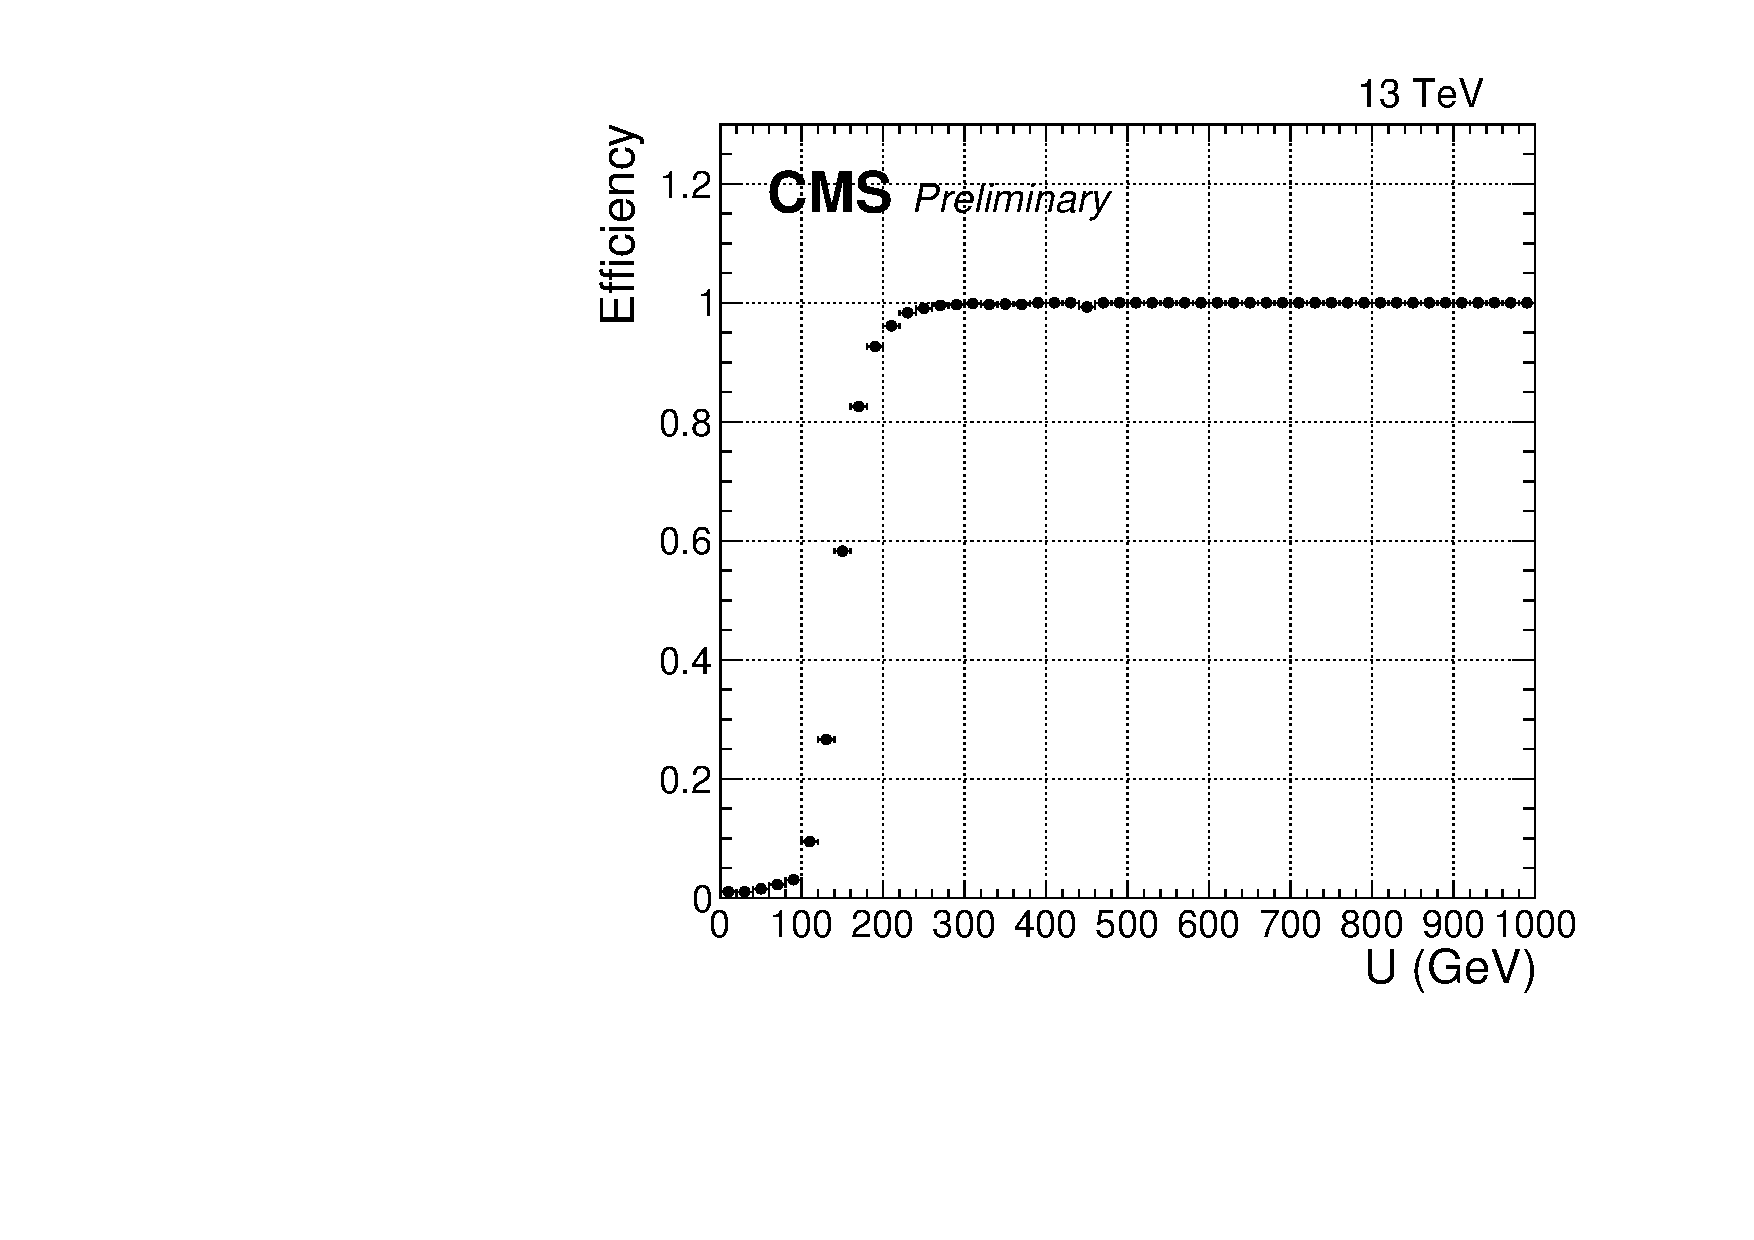
\includegraphics[width=0.475\textwidth]{figures/trigs/met_trig.pdf}
%         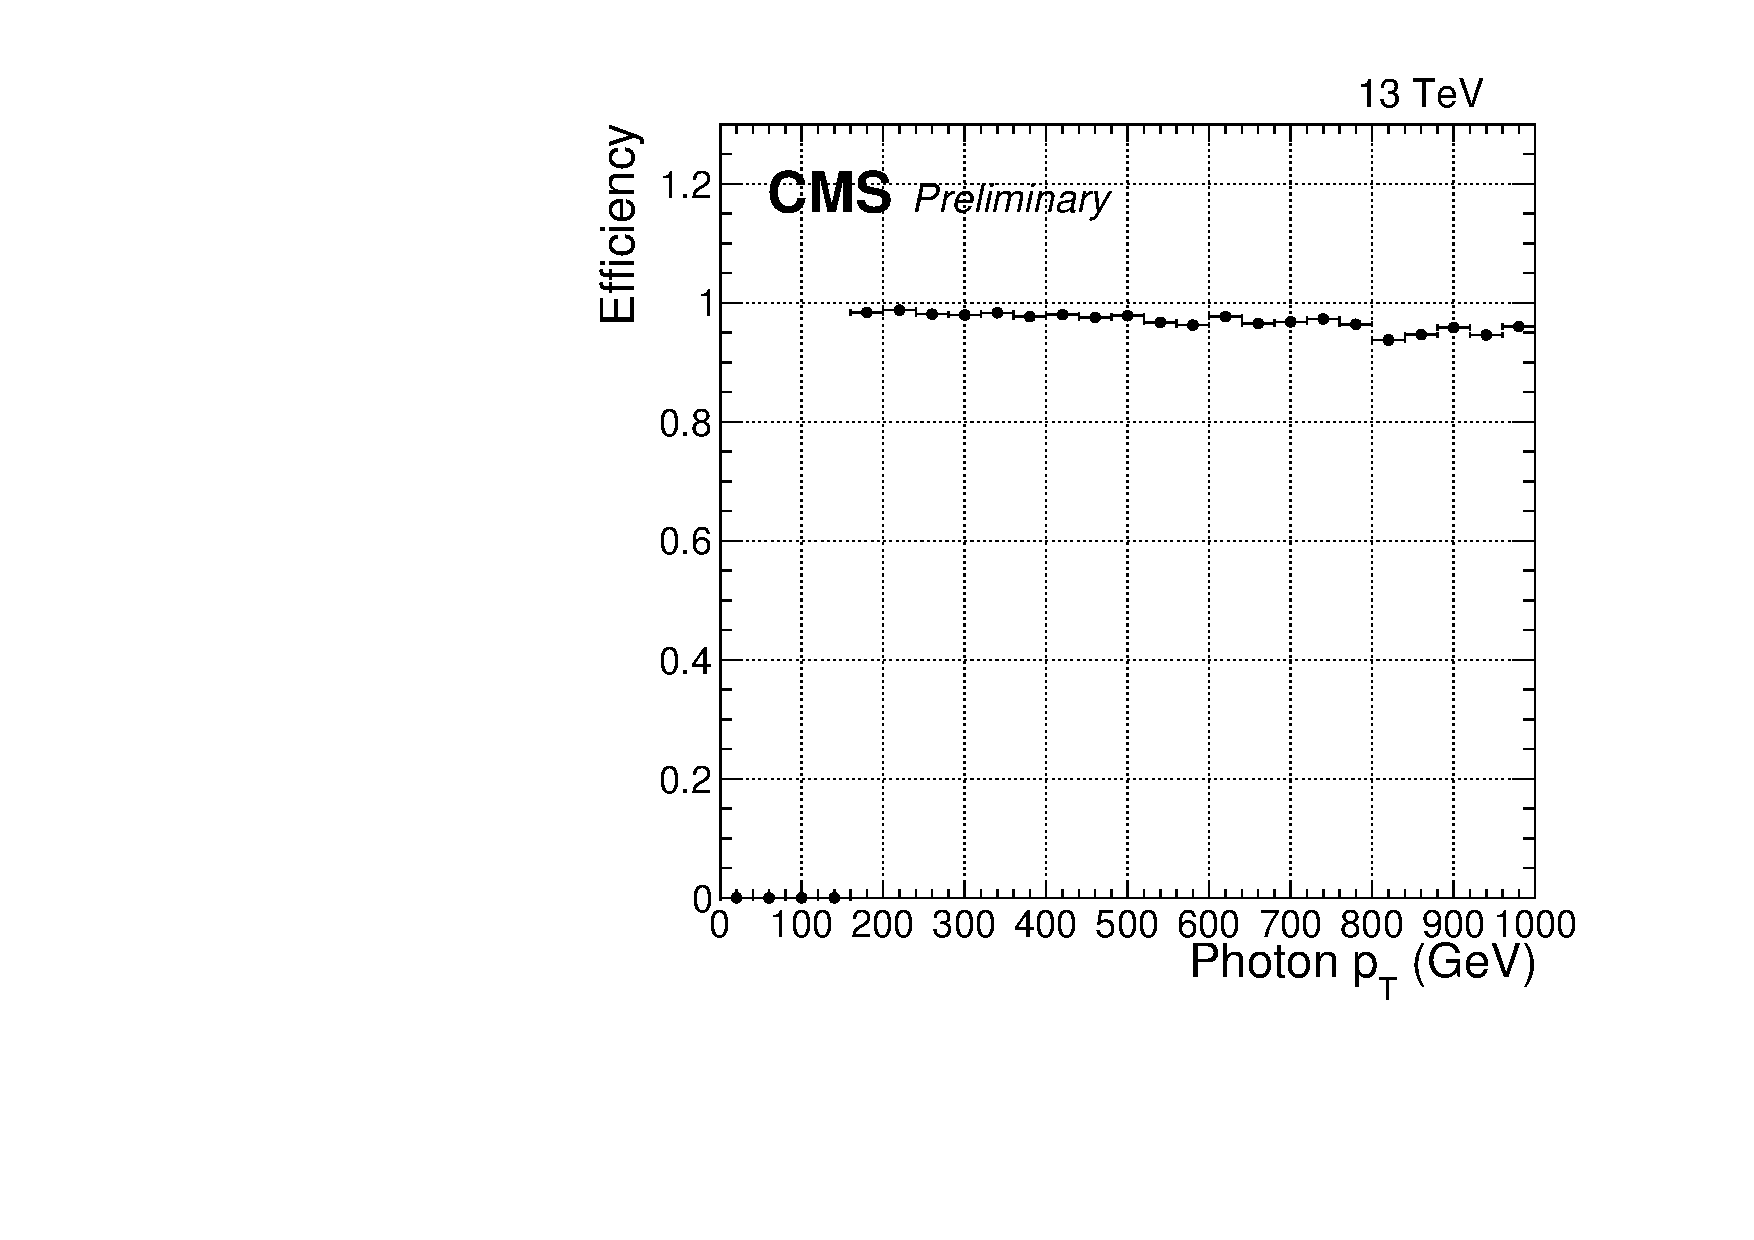
\includegraphics[width=0.475\textwidth]{figures/trigs/photon_trig.pdf}\\
%         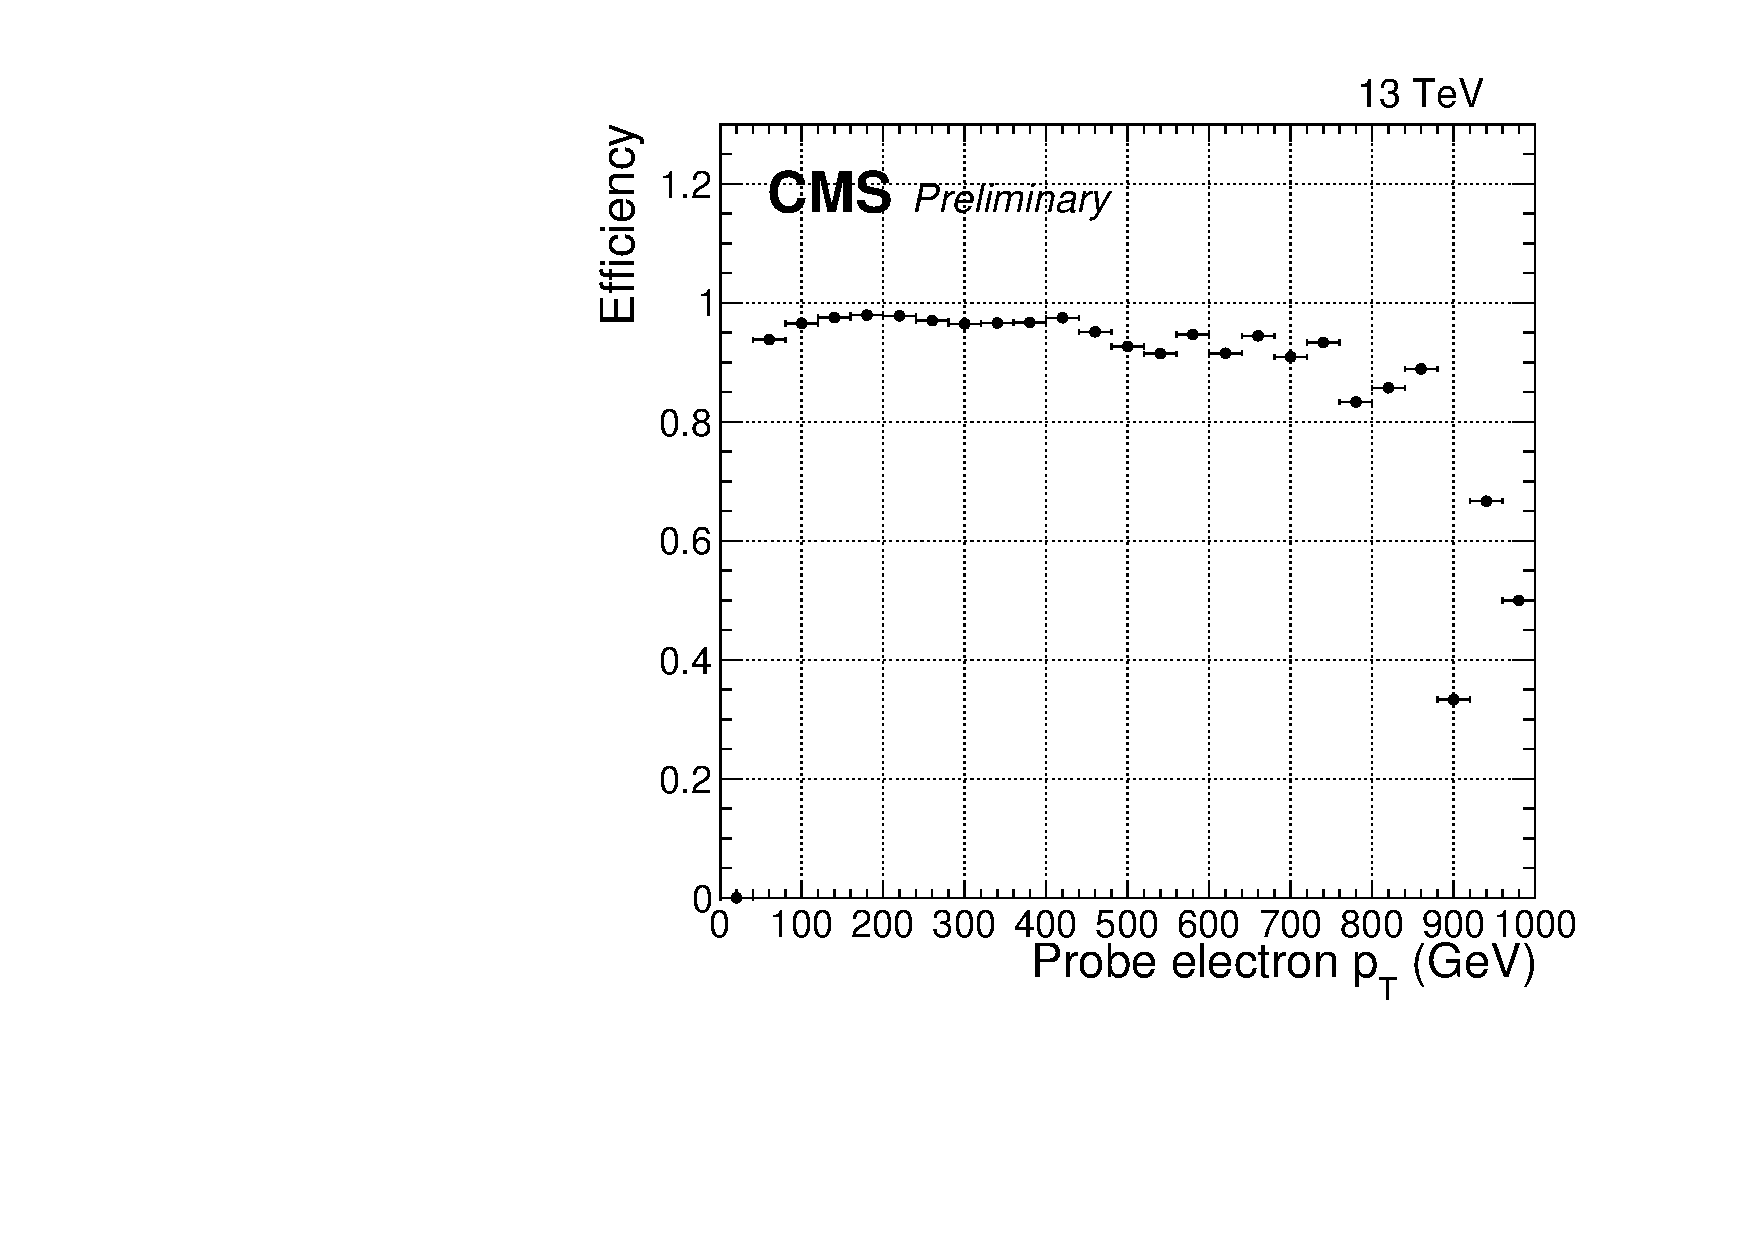
\includegraphics[width=0.475\textwidth]{figures/trigs/electron_barrel_trig.pdf}
%         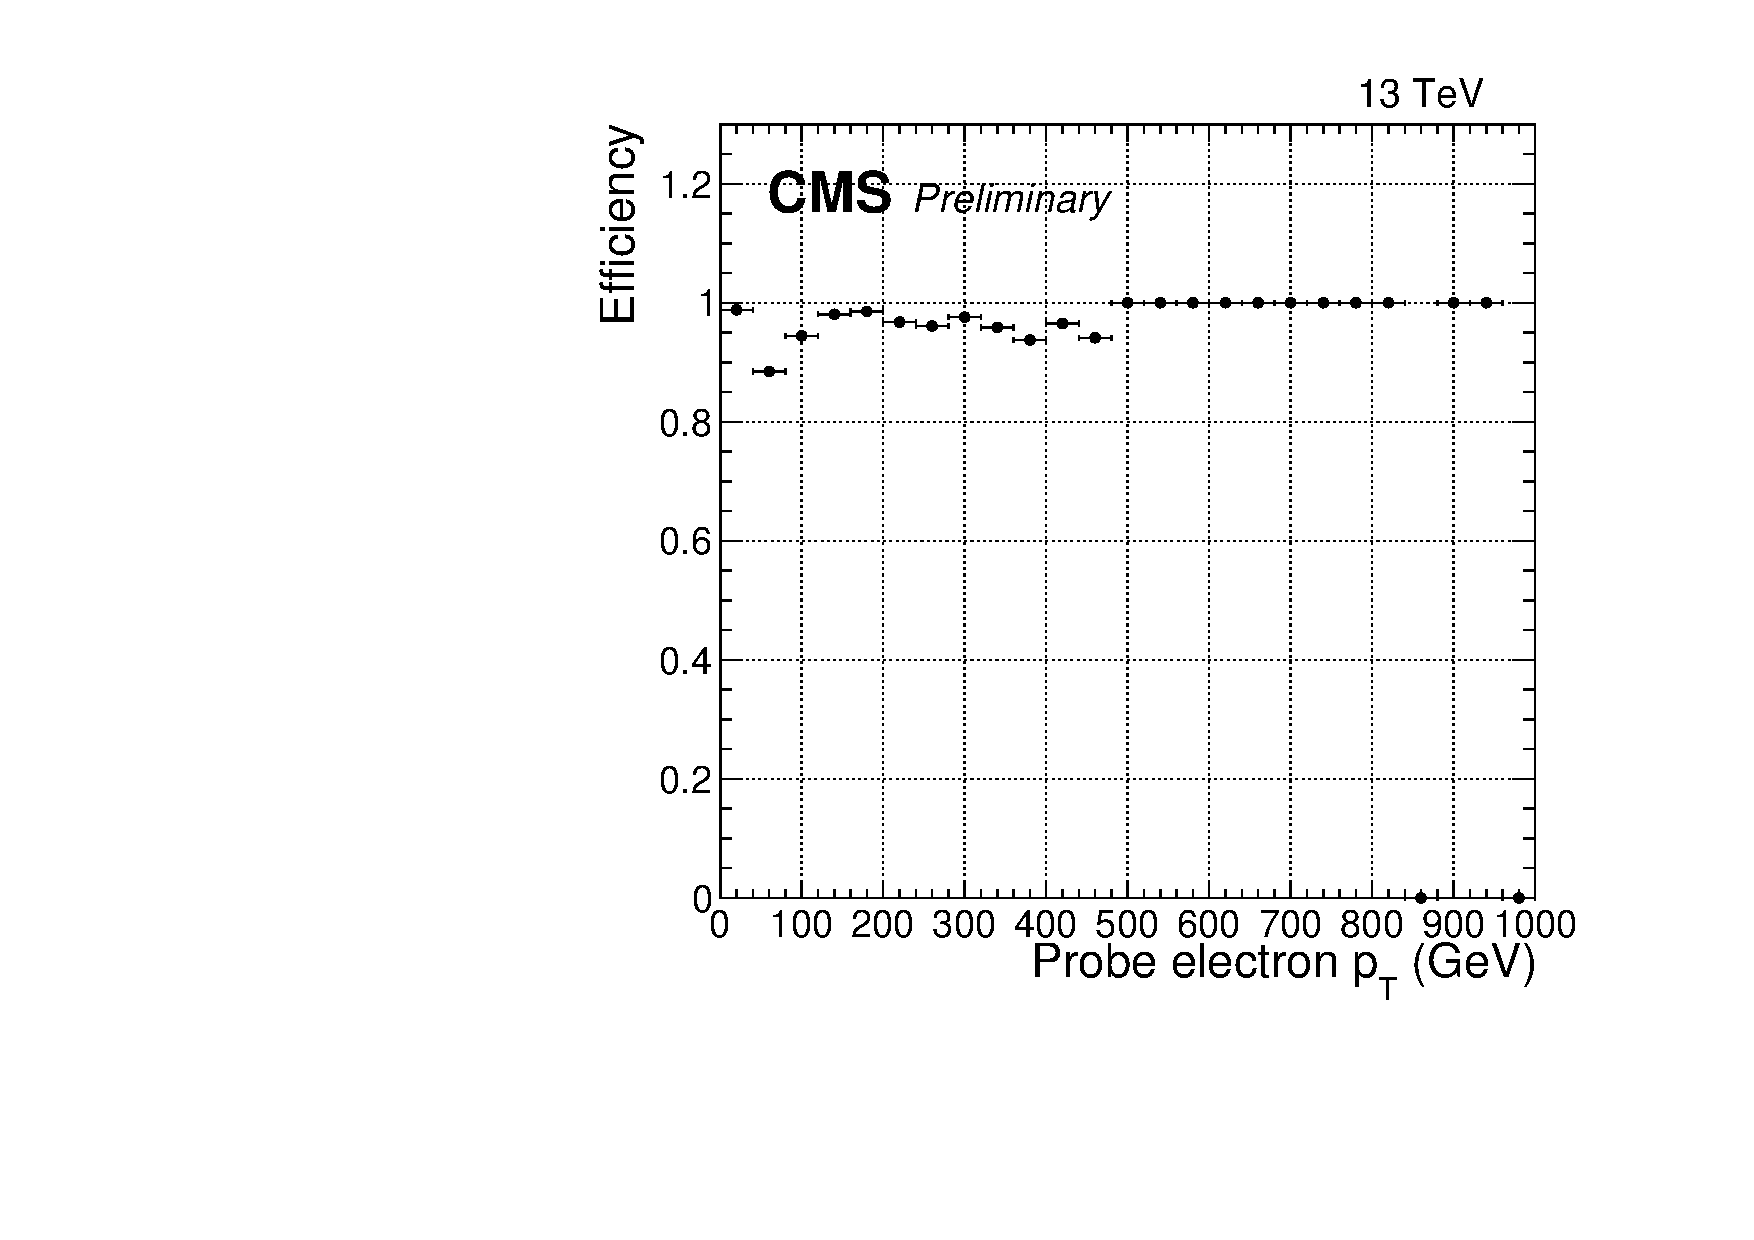
\includegraphics[width=0.475\textwidth]{figures/trigs/electron_endcap_trig.pdf}\\
%         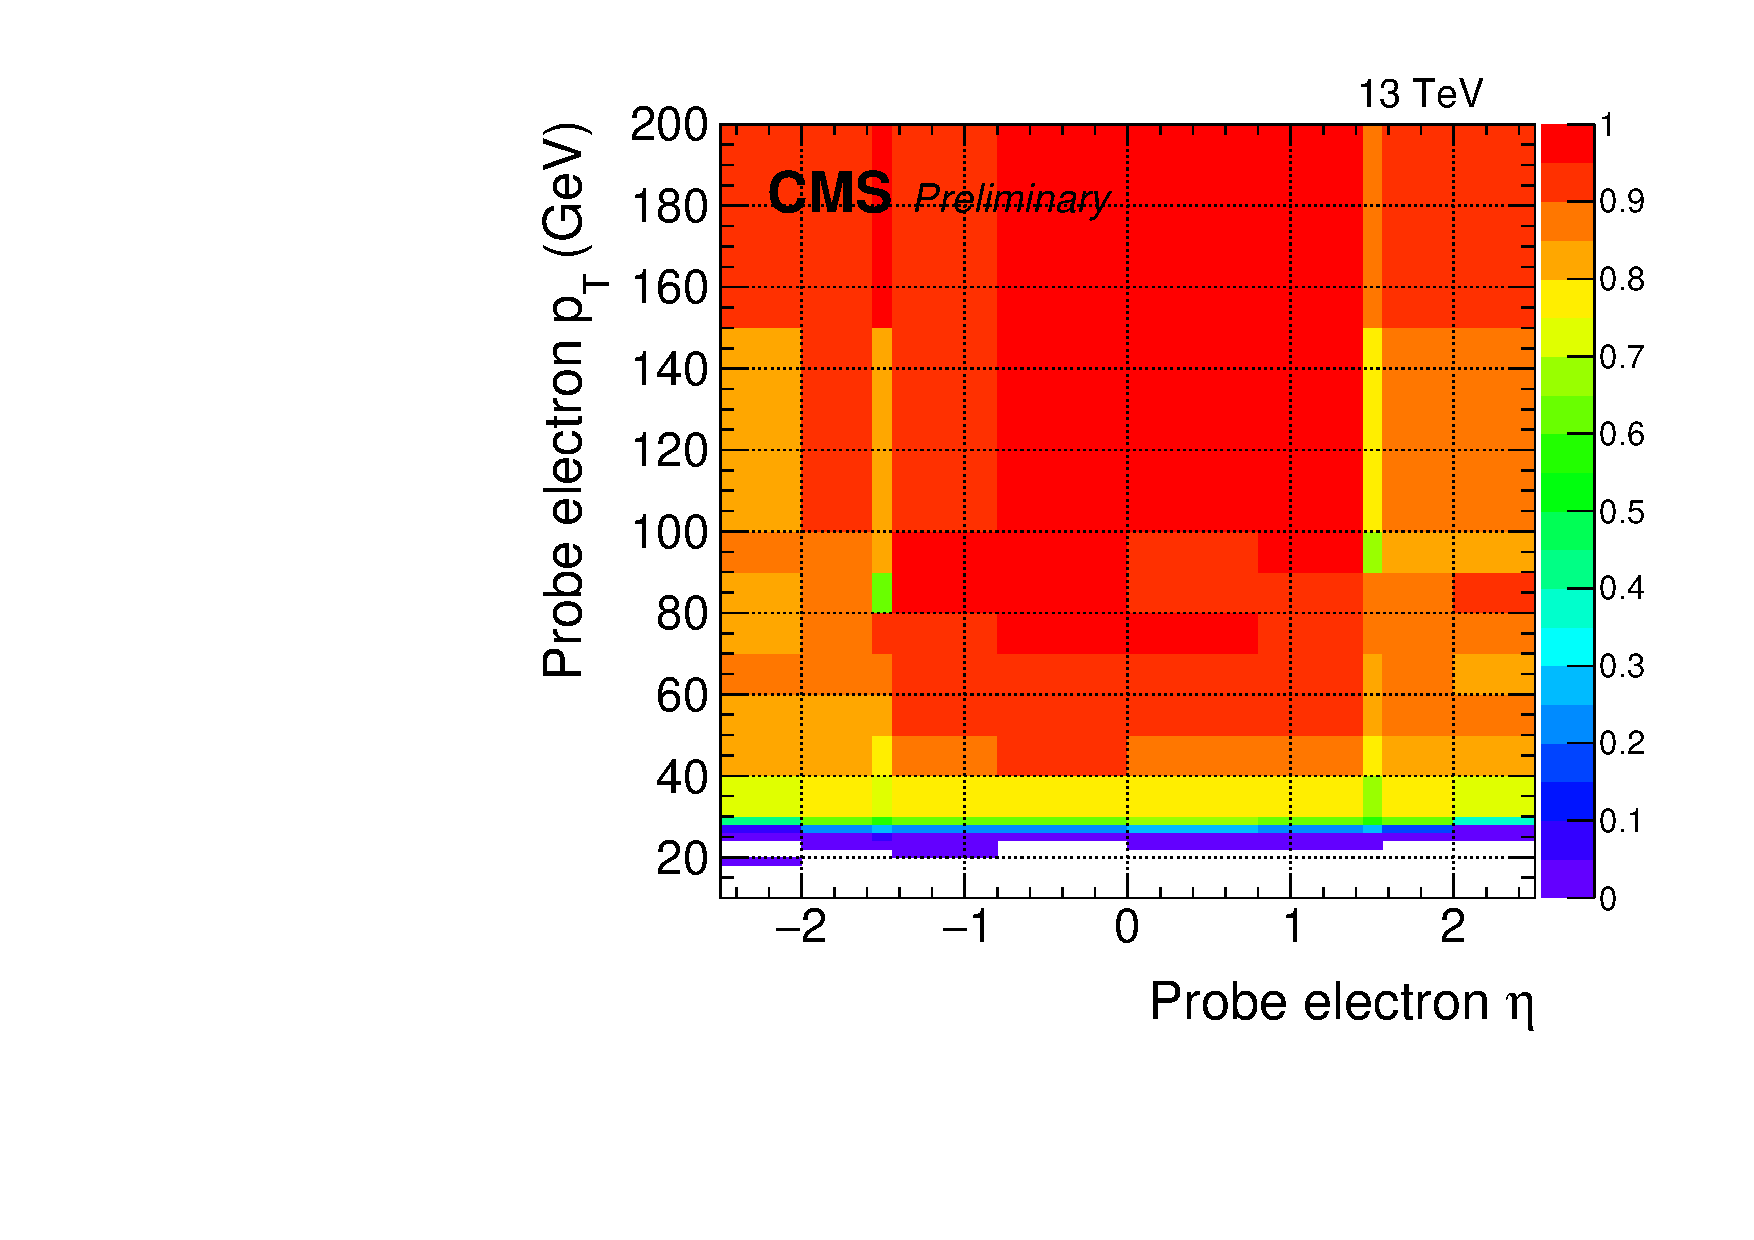
\includegraphics[width=0.475\textwidth]{figures/trigs/electron_lowpt_trig.pdf}\\
%   \caption{Efficiency of MET and METNoMu triggers as a function of offline \ETm~(upper left); efficiency of photon triggers (upper right); efficiency of single electron triggers for barrel/endcap (middle left/right); efficiency of single electron triggers at low $p_\text{T}$ ($<100$\,GeV). 
%   }
%   \label{fig:trigs}
% \end{figure}

\begin{figure}[hbtp]\begin{center}
    \subfloat[][]{
      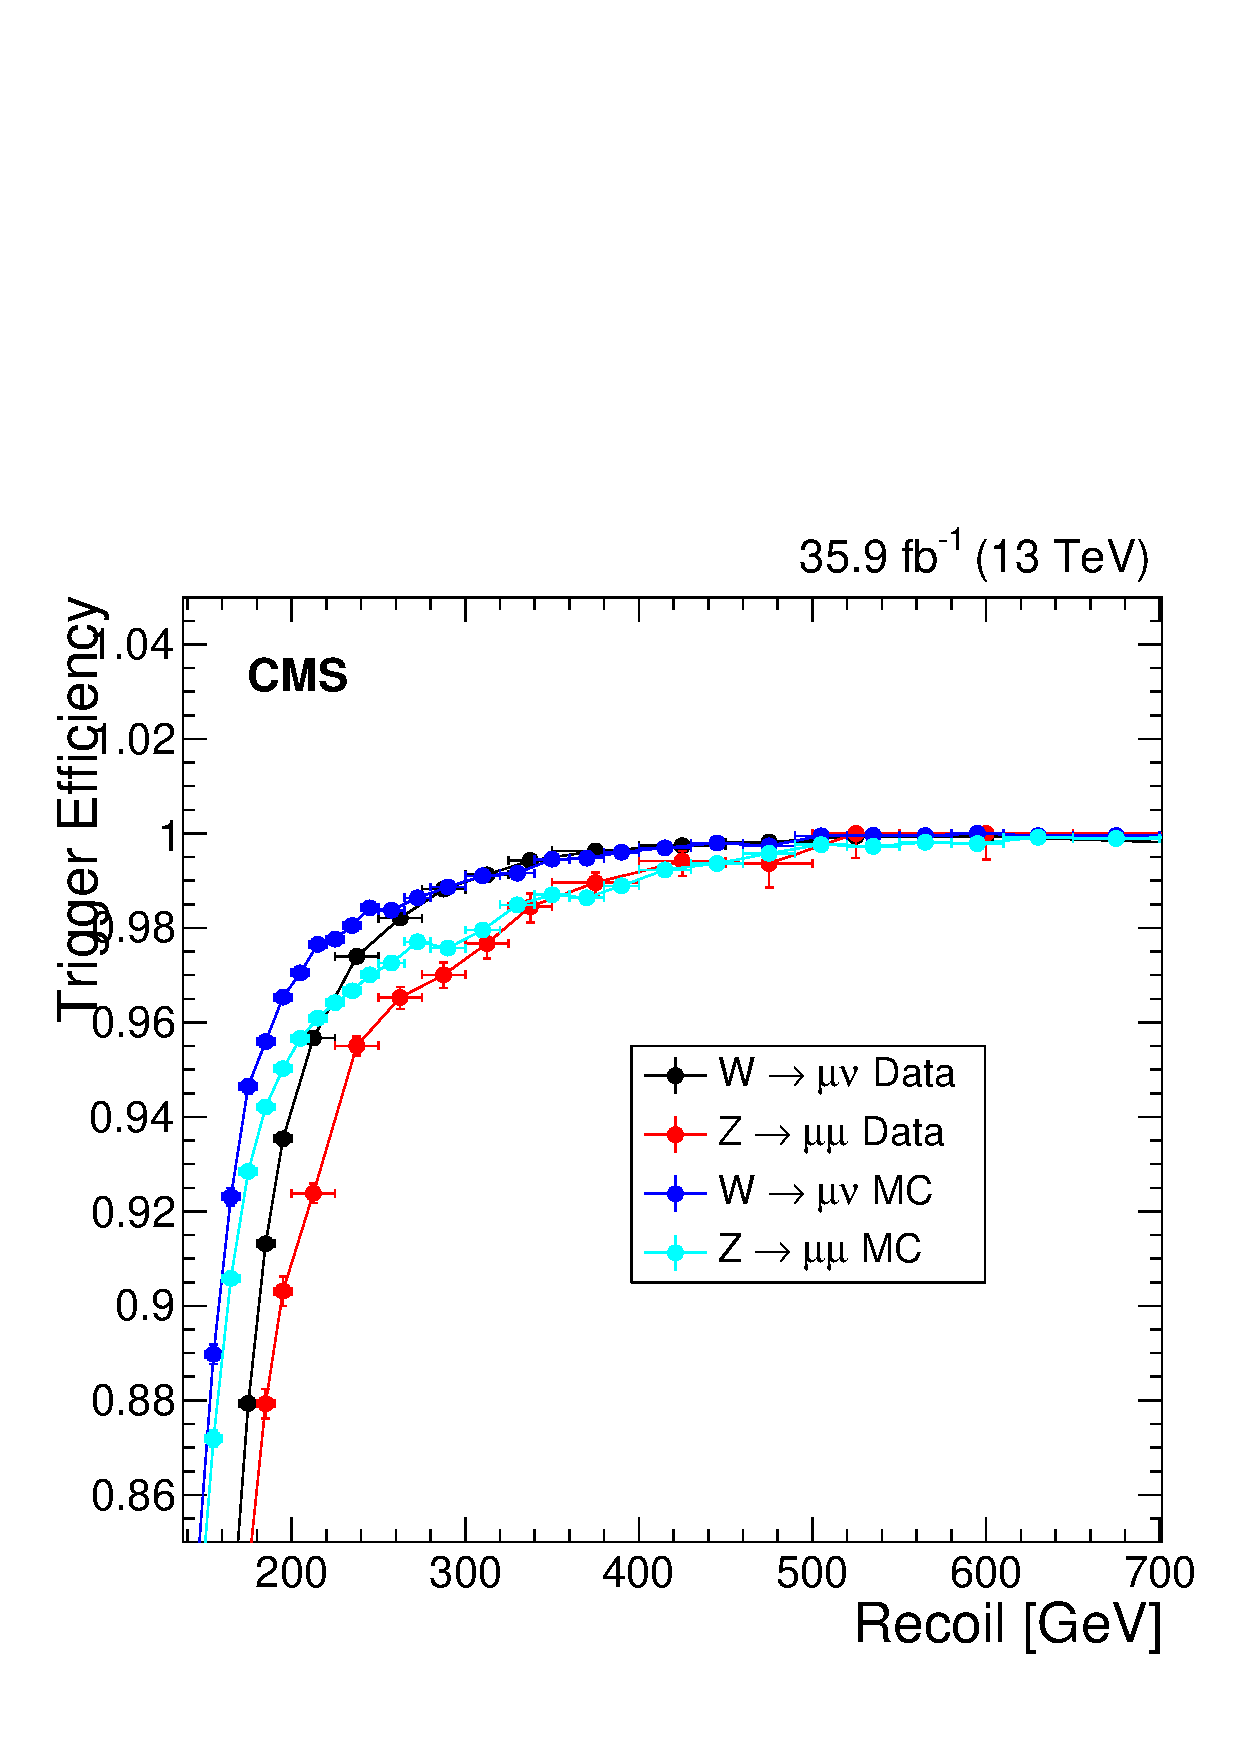
\includegraphics[width=0.45\textwidth]{figures/trigs/comparisonTurnOn_Wmn_Zmm_before_fix.pdf}
    }
    \subfloat[][]{
      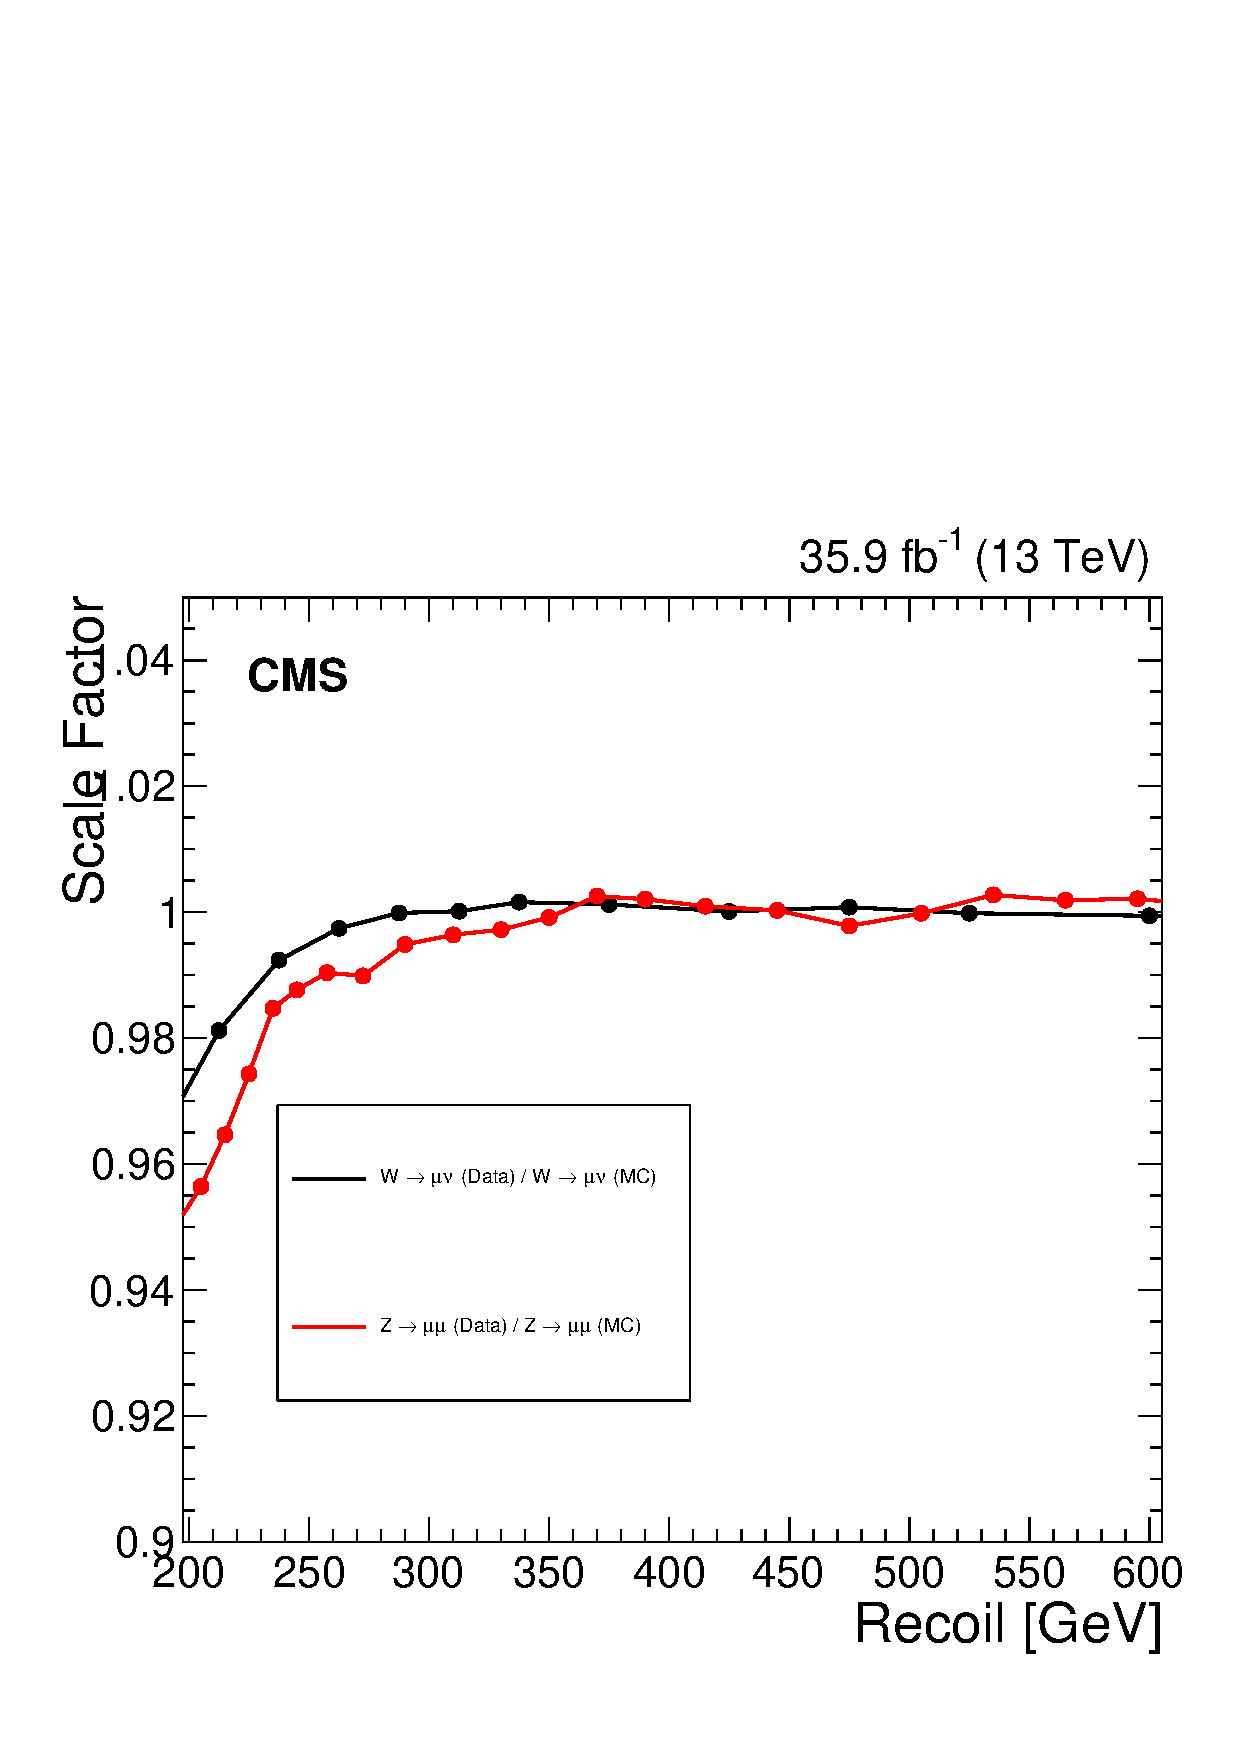
\includegraphics[width=0.45\textwidth]{figures/trigs/scale_factor_trigger_wmn_zmm_before_fix.pdf}
    }
    \caption{Comparison on both data and MC between the METNoMu+MHTNoMu trigger efficiency turn on as measured in \Wmn~and \Zmm~events (left). (Right) Comparison between the data to MC scale factors which show a significant disagreement in the low recoil region; taken from~\cite{CMS_AN_2016-473}.}
\label{fig:triggerComparison_wmn_zmm}\end{center}\end{figure}

\begin{figure}[hbtp]\begin{center}
      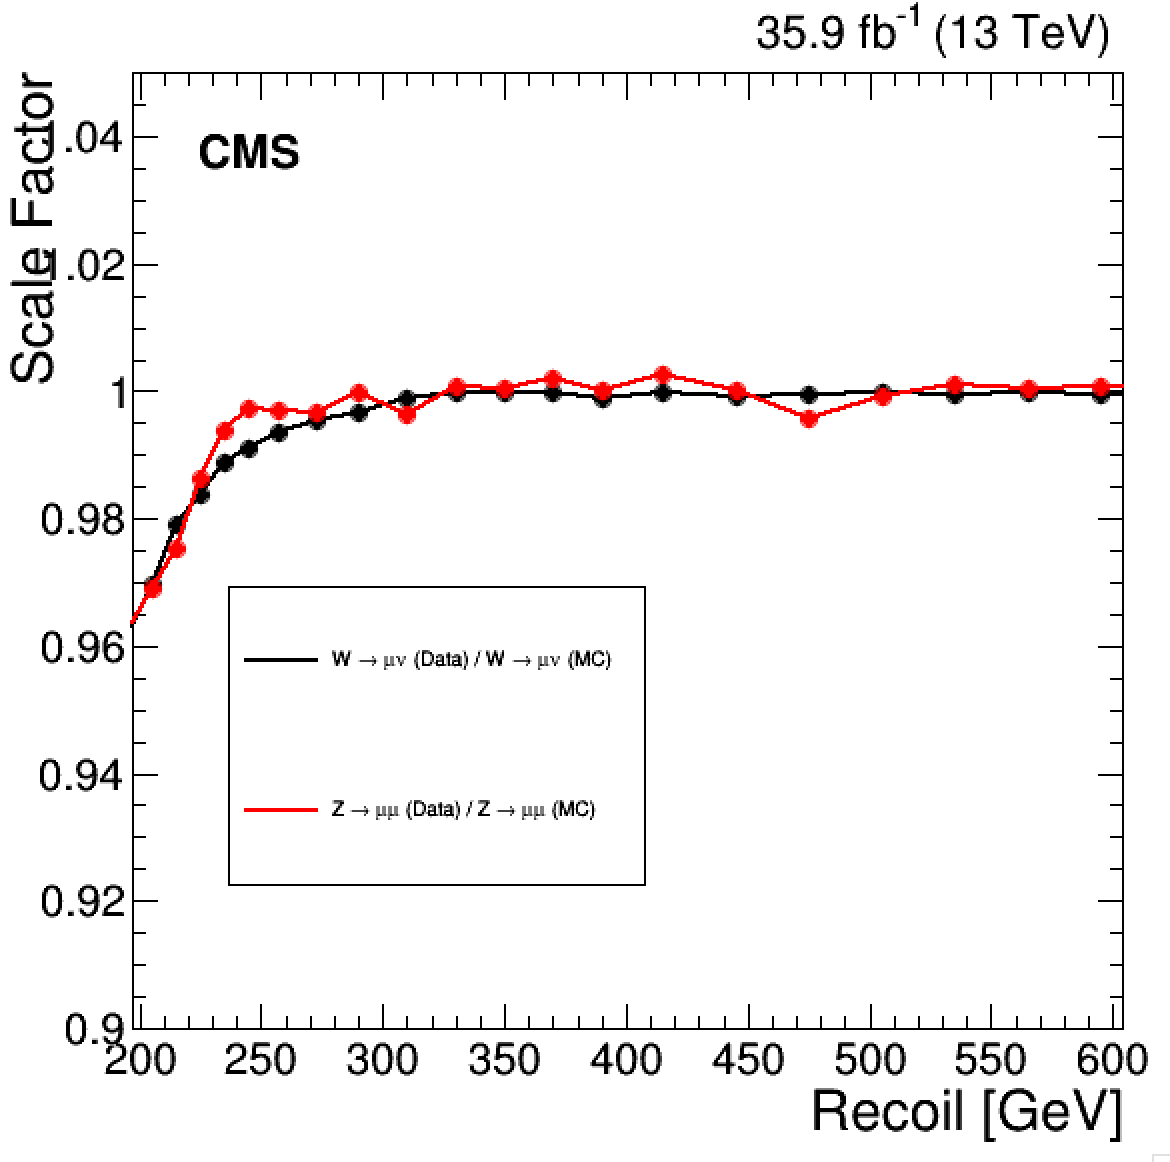
\includegraphics[width=0.45\textwidth]{figures/trigs/scale_factor_trigger_wmn_zmm_after_fix.png}
      \caption{
        Comparison between the data to MC scale factors as obtained computing the MET trigger turn-on in \Wmn~and \Zmm~events, which nicely agree over the full recoil spectrum after requiring to have a number of HLT muons equal to the number of the identified offline muons in the event; taken from~\cite{CMS_AN_2016-473}.}
      \label{fig:trigger_eff_corr}\end{center}\end{figure}

\begin{figure}[hbtp]\begin{center}
      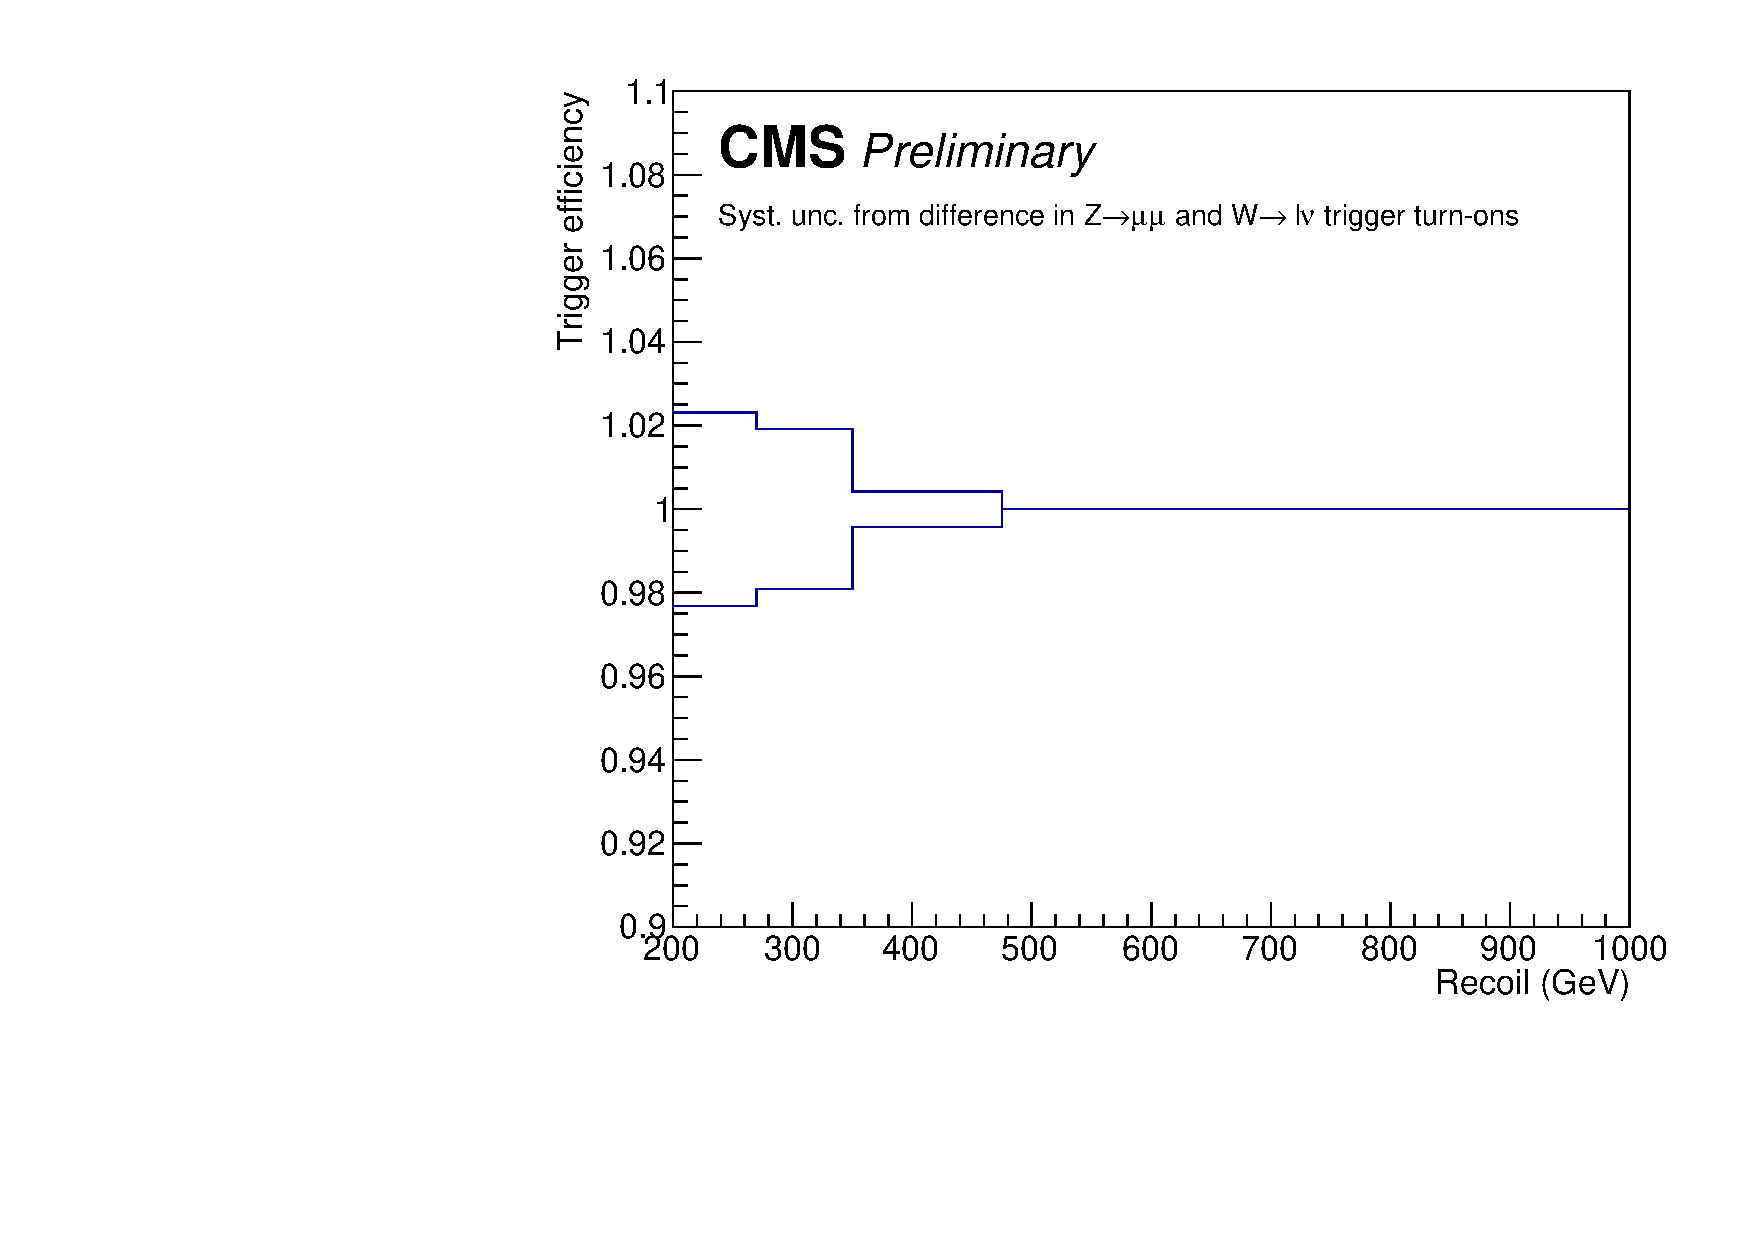
\includegraphics[width=0.45\textwidth]{figures/trigs/fixtrig_monoh.pdf}
      \caption{ Uncertainty on applied trigger weights in the \Zmm~control region due to the different METNoMu+MHTNoMu trigger efficiencies  in \Wmn~and \Zmm~events.
}
      \label{fig:fixtrig_monoh}\end{center}\end{figure}


\begin{figure}[hbtp]\begin{center}
    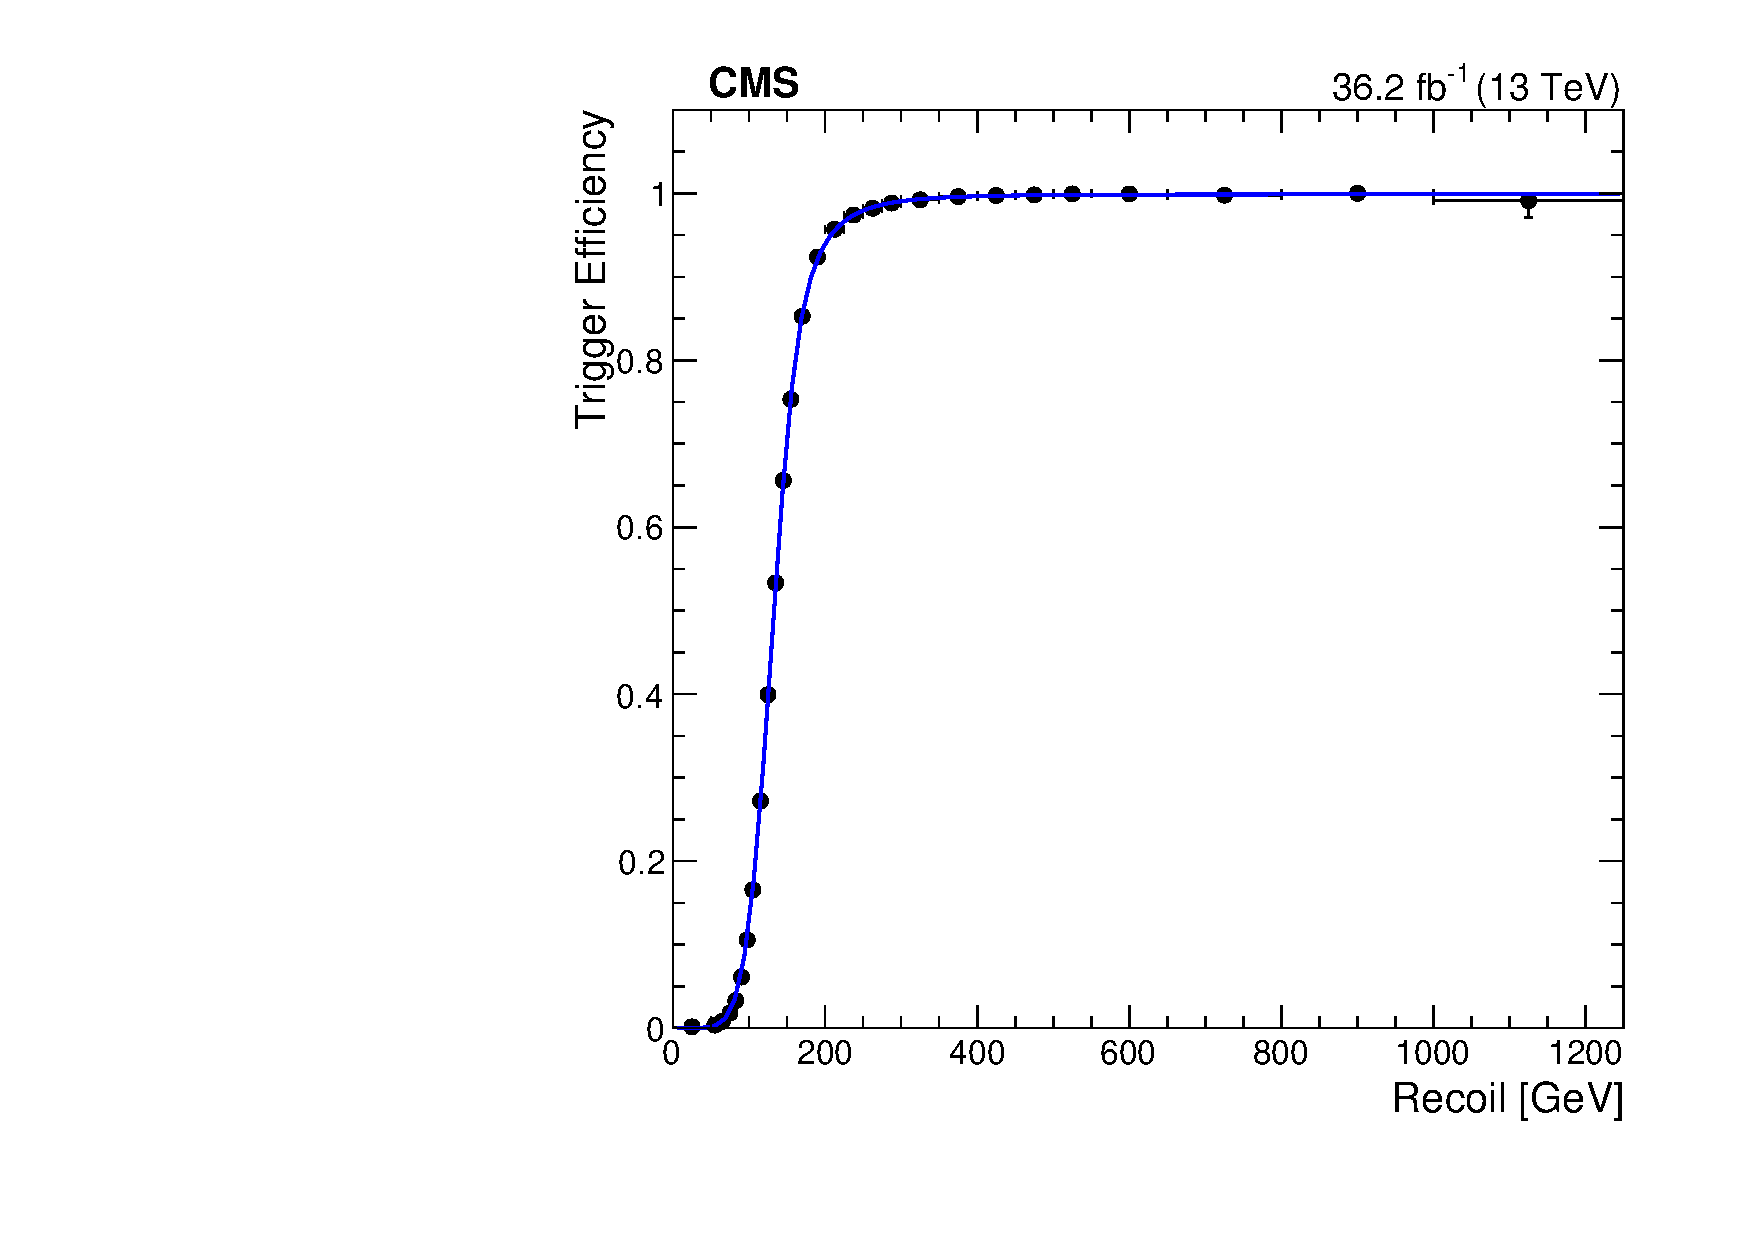
\includegraphics[height=0.45\textwidth,width=0.45\textwidth]{figures/trigs/metTriggerEff_mu.pdf}
    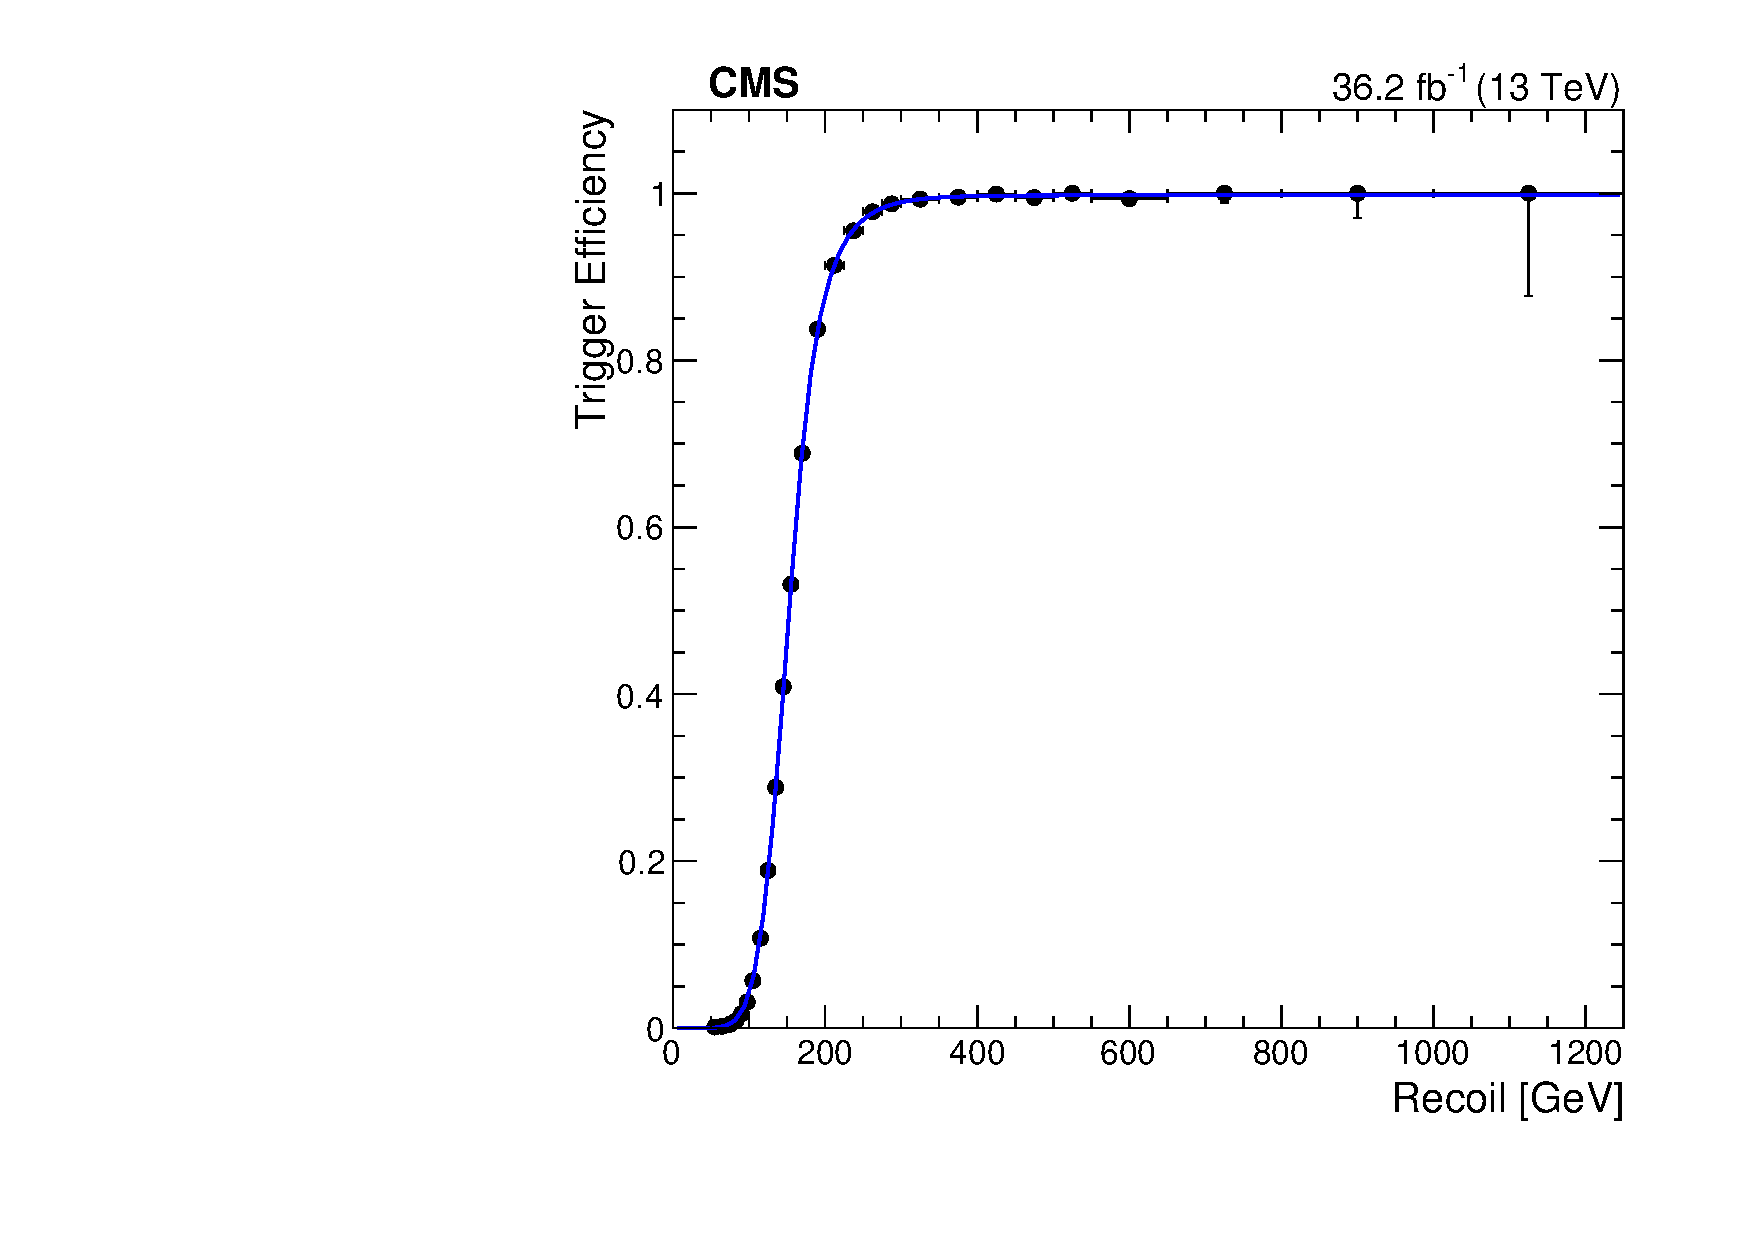
\includegraphics[height=0.45\textwidth,width=0.45\textwidth]{figures/trigs/metTriggerEff_el.pdf}
        \caption{MET trigger turn-on curve measured in single muon events (left) and single electron events (right). In the case of the single muon events, the trigger turn-on is computed as a function of the recoil (\MET without including the muon), while in the case of the single electron events it is computed as a function of \MET. Both measurements agree at the 1-2\% level at higher MET, and the efficiencies from the measurement in single muon events are applied to the simulated events in the analysis; taken from~\cite{CMS_AN_2016-473}. }
    \label{fig:hlteff_met}
 \end{center}\end{figure}


\begin{figure}[h!]
  \begin{center}
          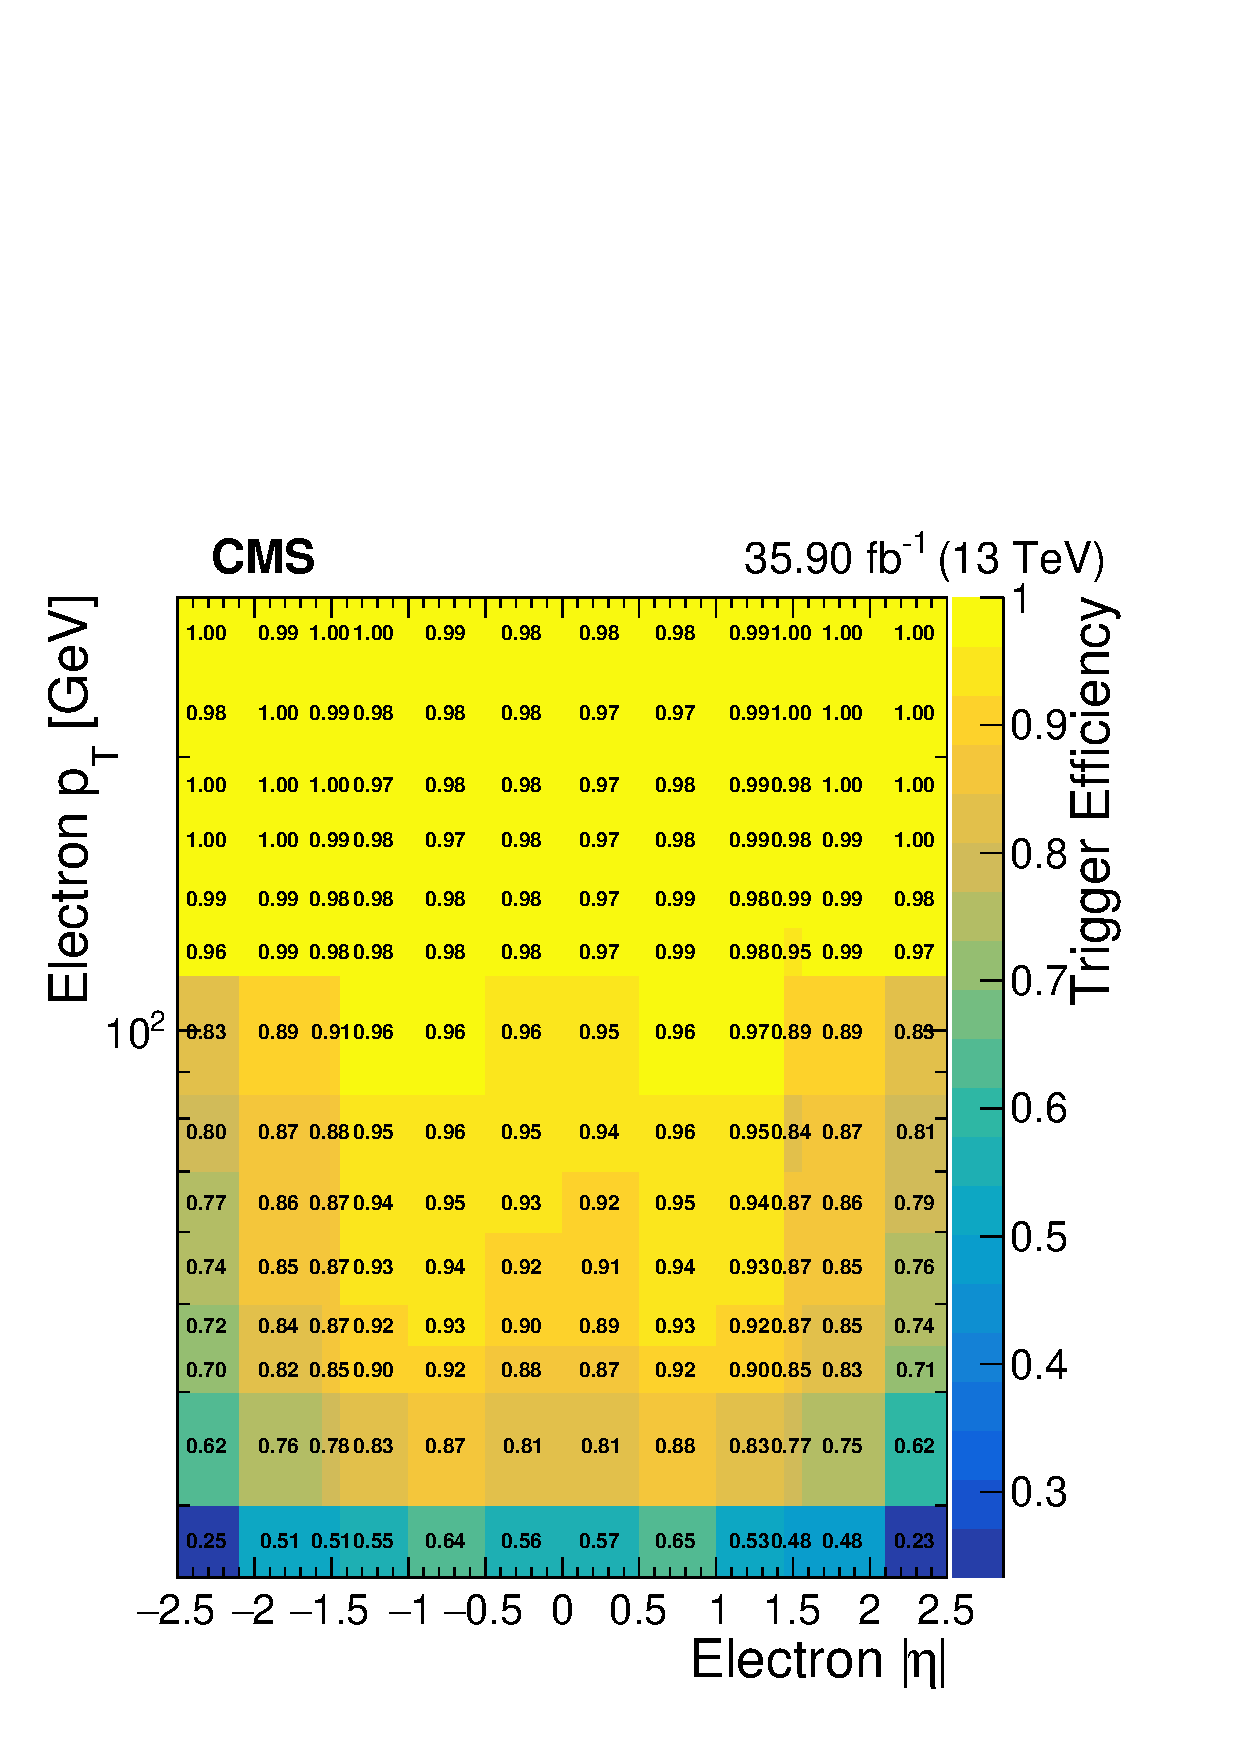
\includegraphics[width=0.40\textwidth]{figures/trigs/trgeff_ele_pt35.pdf}
          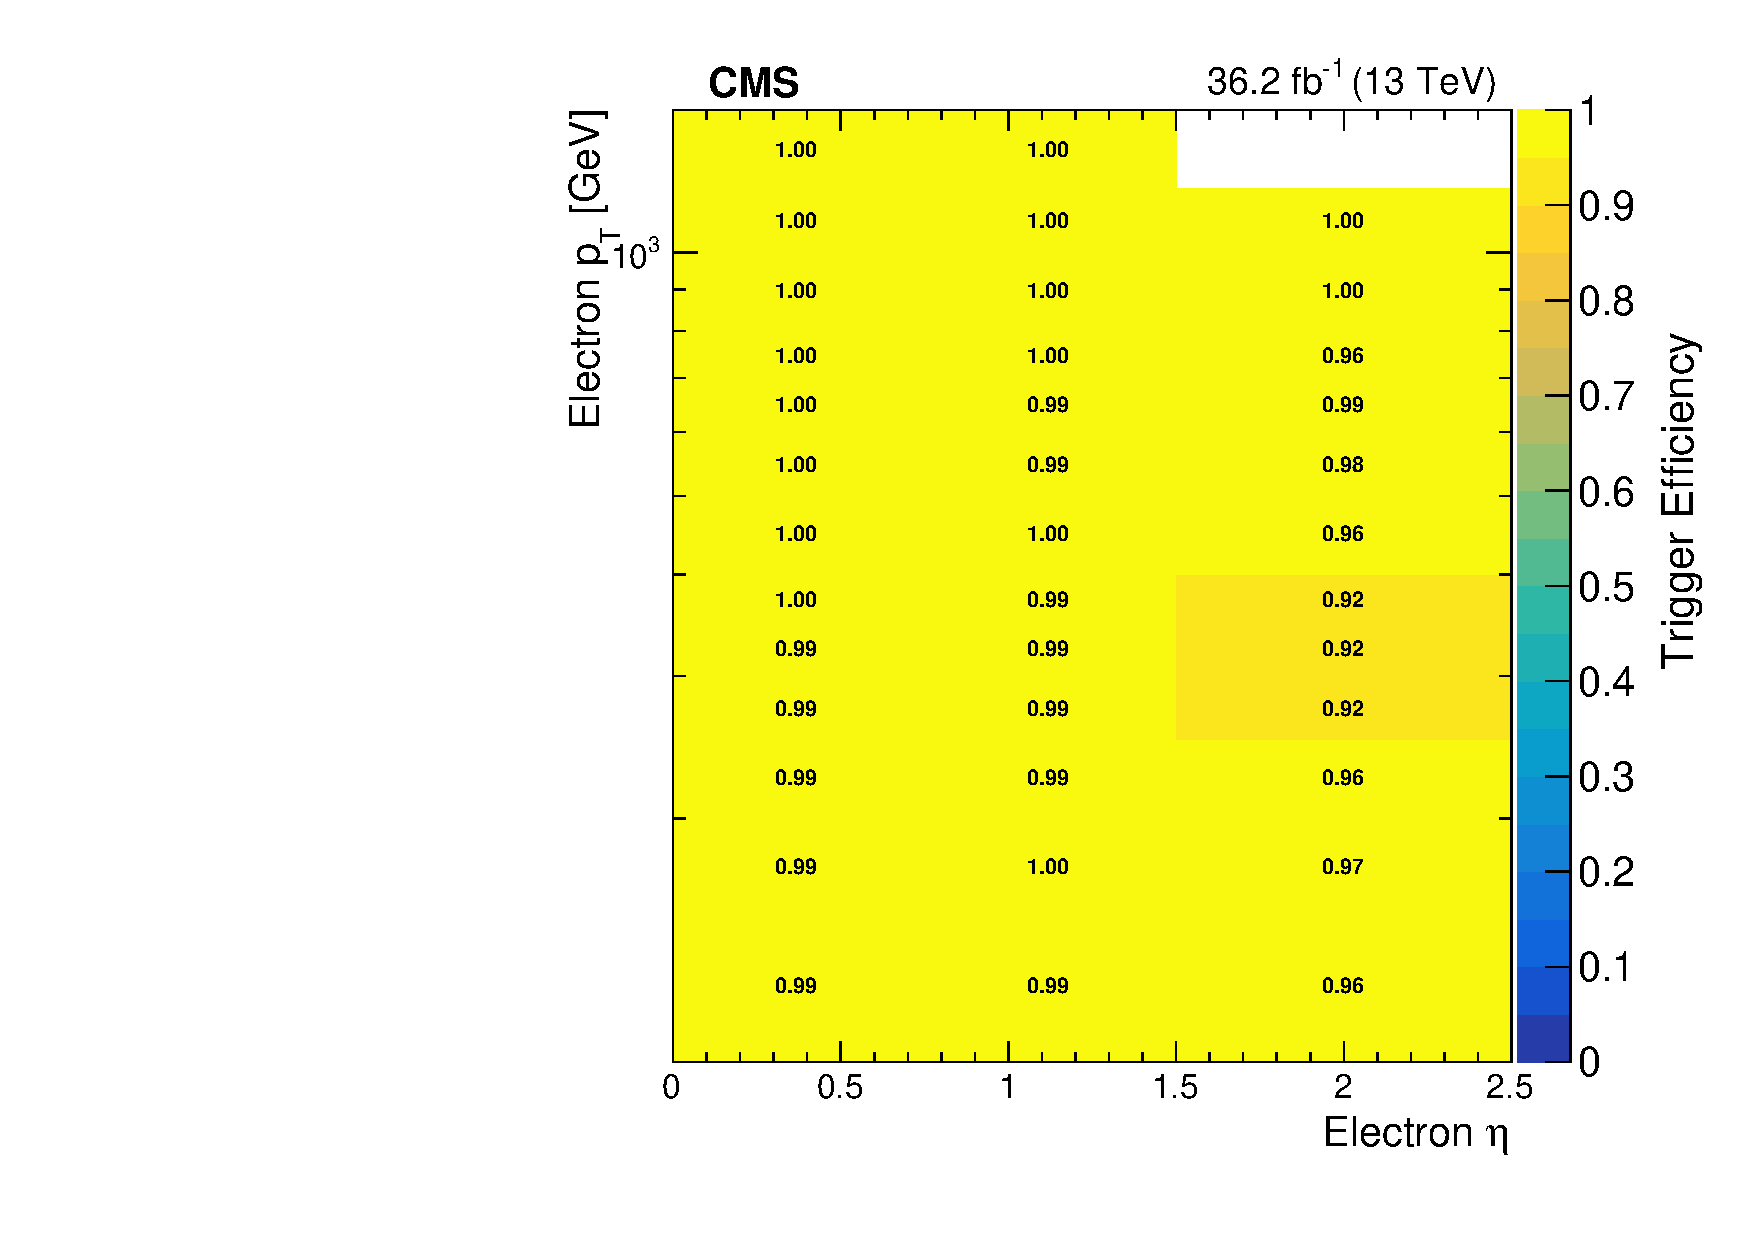
\includegraphics[width=0.42\textwidth]{figures/trigs/effetapt_jetht.pdf}
   \caption{Single electron trigger efficiencies as a function of electron \pt and $\eta$. The left plot shows the trigger efficiencies measured using Z tag-n-probe starting with electron \pt of 20 \GeV. The right one shows the electron trigger efficiency measured in the JetHT dataset using events passing the PFHT650 or PFHT800 trigger, starting at electron \pt of 100 \GeV; taken from~\cite{CMS_AN_2016-473}.}
   \label{fig:eltrigsfsplot}
  \end{center}
\end{figure}


\subsection{Background Monte Carlo Samples}

A list of all background MC samples and the corresponding cross-sections are given in Table~\ref{tab:bgmc}

{ \footnotesize

\centering
\begin{table}[htbp]\footnotesize
\begin{center}
  \caption{List of background MC samples. Datasets marked with * are LO in QCD and EWK but will have NLO corrections applied. Cross-sections marked with $\dag$ are (N)NLO} \label{tab:bgmc}
\begin{tabular}{|l|c|}
  \hline
  Dataset name & $\sigma$ [pb] \\
  \hline
/QCD\_HT200to300\_TuneCUETP8M1\_13TeV-madgraphMLM-pythia8 & $1735000$\\
/QCD\_HT300to500\_TuneCUETP8M1\_13TeV-madgraphMLM-pythia8 & $366800$\\
/QCD\_HT500to700\_TuneCUETP8M1\_13TeV-madgraphMLM-pythia8 & $29370$\\
/QCD\_HT700to1000\_TuneCUETP8M1\_13TeV-madgraphMLM-pythia8 & $6524$\\
/QCD\_HT1000to1500\_TuneCUETP8M1\_13TeV-madgraphMLM-pythia8 & $1064$\\
/QCD\_HT1500to2000\_TuneCUETP8M1\_13TeV-madgraphMLM-pythia8 & $121.5$\\
/QCD\_HT2000toInf\_TuneCUETP8M1\_13TeV-madgraphMLM-pythia8 & $25.42$\\
/ST\_t-channel\_top\_4f\_inclusiveDecays\_13TeV-powhegV2-madspin-pythia8\_TuneCUETP8M1 & $136.02^\dag$\\
/ST\_t-channel\_antitop\_4f\_inclusiveDecays\_13TeV-powhegV2-madspin-pythia8\_TuneCUETP8M1 & $80.95^\dag$\\
/ST\_tW\_antitop\_5f\_inclusiveDecays\_13TeV-powheg-pythia8\_TuneCUETP8M1 & $35.85^\dag$\\
/ST\_tW\_top\_5f\_inclusiveDecays\_13TeV-powheg-pythia8\_TuneCUETP8M1 & $35.85^\dag$\\
/ZH\_HToBB\_ZToNuNu\_M125\_13TeV\_powheg\_pythia8 & $0.08912$ \\
/ZH\_HToBB\_ZToLL\_M125\_13TeV\_powheg\_pythia8 & $0.04865$ \\
/ggZH\_HToBB\_ZToNuNu\_M125\_13TeV\_powheg\_pythia8 & $0.014366$ \\
/ggZH\_HToBB\_ZToLL\_M125\_13TeV\_powheg\_pythia8 & $0.007842$ \\
/WminusH\_HToBB\_WToLNu\_M125\_13TeV\_powheg\_pythia8 & $0.100$ \\
/WplusH\_HToBB\_WToLNu\_M125\_13TeV\_powheg\_pythia8 & $0.159$ \\
/ttHTobb\_M125\_13TeV\_powheg\_pythia8 & $0.506*0.5824$\\
/TT\_TuneCUETP8M2T4\_13TeV-powheg-pythia8 & $831.76^\dag$\\
/WW\_TuneCUETP8M1\_13TeV-pythia8 & $118.7^\dag$\\
/WZ\_TuneCUETP8M1\_13TeV-pythia8 & $47.2^\dag$\\
/ZZ\_TuneCUETP8M1\_13TeV-pythia8 & $16.6^\dag$\\
/DYJetsToLL\_M-50\_HT-100to200\_TuneCUETP8M1\_13TeV-madgraphMLM-pythia8* & $148.0$\\
/DYJetsToLL\_M-50\_HT-200to400\_TuneCUETP8M1\_13TeV-madgraphMLM-pythia8* & $40.94$\\
/DYJetsToLL\_M-50\_HT-400to600\_TuneCUETP8M1\_13TeV-madgraphMLM-pythia8* & $5.497$\\
/DYJetsToLL\_M-50\_HT-600to800\_TuneCUETP8M1\_13TeV-madgraphMLM-pythia8* & $1.367$\\
/DYJetsToLL\_M-50\_HT-800to1200\_TuneCUETP8M1\_13TeV-madgraphMLM-pythia8* & $0.6304$\\
/DYJetsToLL\_M-50\_HT-1200to2500\_TuneCUETP8M1\_13TeV-madgraphMLM-pythia8* & $0.1514$\\
/DYJetsToLL\_M-50\_HT-2500toInf\_TuneCUETP8M1\_13TeV-madgraphMLM-pythia8* & $0.003565$\\
/WJetsToLNu\_HT-100To200\_TuneCUETP8M1\_13TeV-madgraphMLM-pythia8* & $1343$\\
/WJetsToLNu\_HT-200To400\_TuneCUETP8M1\_13TeV-madgraphMLM-pythia8* & $359.6$\\
/WJetsToLNu\_HT-400To600\_TuneCUETP8M1\_13TeV-madgraphMLM-pythia8* & $48.85$\\
/WJetsToLNu\_HT-600To800\_TuneCUETP8M1\_13TeV-madgraphMLM-pythia8* & $12.05$ \\
/WJetsToLNu\_HT-800To1200\_TuneCUETP8M1\_13TeV-madgraphMLM-pythia8* & $5.501$ \\
/WJetsToLNu\_HT-1200To2500\_TuneCUETP8M1\_13TeV-madgraphMLM-pythia8* & $1.329$ \\
/WJetsToLNu\_HT-2500ToInf\_TuneCUETP8M1\_13TeV-madgraphMLM-pythia8* & $0.03216$ \\
/ZJetsToNuNu\_HT-100To200\_13TeV-madgraph* & $280.5$ \\
/ZJetsToNuNu\_HT-200To400\_13TeV-madgraph* & $77.7$\\
/ZJetsToNuNu\_HT-400To600\_13TeV-madgraph* & $10.71$\\
/ZJetsToNuNu\_HT-600To800\_13TeV-madgraph* & $2.559$\\ 
/ZJetsToNuNu\_HT-800To1200\_13TeV-madgraph* & $1.183$\\
/ZJetsToNuNu\_HT-1200To2500\_13TeV-madgraph* & $0.292$\\
/ZJetsToNuNu\_HT-2500ToInf\_13TeV-madgraph* & $0.0069$ \\
  \hline
  \end{tabular}
  \end{center}
\end{table}

}

NLO QCD and electroweak correction factors are applied to the W and Z
boson samples depending on the boson $\pt$. They are listed in
Tab.~\ref{tab:nlokfacw} and Tab.~\ref{tab:nlokfacz}.


\begin{table}[htbp]
\centering
  \caption{NLO $k$ factors for QCD and EW corrections for the W+jets simulation, depending on the \pt of the generated W boson.} \label{tab:nlokfacw}
  \begin{tabular}{cccc}
  \hline
  From W \pt & to W \pt & QCD $k$ factor & EW $k$ factor\\
  \hline
150 & 170 & 1.43896 & 0.966481 \\
170 & 200 & 1.45307 & 0.958351 \\
200 & 230 & 1.41551 & 0.948513 \\
230 & 260 & 1.42199 & 0.938304 \\
260 & 290 & 1.3477 & 0.929394 \\
290 & 320 & 1.35302 & 0.919688 \\
320 & 350 & 1.34289 & 0.910425 \\
350 & 390 & 1.32474 & 0.900288 \\
390 & 430 & 1.23267 & 0.889122 \\
430 & 470 & 1.22641 & 0.877255 \\
470 & 510 & 1.23149 & 0.86653 \\
510 & 550 & 1.21593 & 0.856032 \\
550 & 590 & 1.16506 & 0.84536 \\
590 & 640 & 1.01718 & 0.834675 \\
640 & 690 & 1.01575 & 0.822288 \\
690 & 740 & 1.05425 & 0.810779 \\
740 & 790 & 1.05992 & 0.799689 \\
790 & 840 & 1.01503 & 0.788566 \\
840 & 900 & 1.01761 & 0.777413 \\
900 & 960 & 0.947195 & 0.765405 \\
960 & 1020 & 0.932754 & 0.753711 \\
1020 & 1090 & 1.00849 & 0.742262 \\
1090 & 1160 & 0.94805 & 0.72925 \\
1160 & 1250 & 0.86956 & 0.716423 \\
  \hline
  \end{tabular}
\end{table}



\begin{table}[htbp]
\centering
  \caption{NLO $k$ factors for QCD and EW corrections for the Z+jets simulation, depending on the \pt of the generated Z boson.} \label{tab:nlokfacz}
  \begin{tabular}{cccc}
  \hline
  From Z \pt & to Z \pt & QCD $k$ factor & EW $k$ factor \\
  \hline
150 & 170 & 1.47528 & 0.970592 \\
170 & 200 & 1.5428 & 0.964424 \\
200 & 230 & 1.49376 & 0.956695 \\
230 & 260 & 1.39119 & 0.948747 \\
260 & 290 & 1.40538 & 0.941761 \\
290 & 320 & 1.44661 & 0.934246 \\
320 & 350 & 1.38176 & 0.927089 \\
350 & 390 & 1.37381 & 0.919181 \\
390 & 430 & 1.29145 & 0.909926 \\
430 & 470 & 1.33452 & 0.900911 \\
470 & 510 & 1.25765 & 0.892561 \\
510 & 550 & 1.24265 & 0.884353 \\
550 & 590 & 1.24331 & 0.8761 \\
590 & 640 & 1.16187 & 0.867687 \\
640 & 690 & 1.07349 & 0.858047 \\
690 & 740 & 1.10748 & 0.849014 \\
740 & 790 & 1.06617 & 0.840317 \\
790 & 840 & 1.05616 & 0.832017 \\
840 & 900 & 1.1149 & 0.823545 \\
900 & 960 & 1.03164 & 0.814596 \\
960 & 1020 & 1.06872 & 0.806229 \\
1020 & 1090 & 0.981645 & 0.798038 \\
1090 & 1160 & 0.81729 & 0.789694 \\
1160 & 1250 & 0.924246 & 0.781163 \\
  \hline
  \end{tabular}
\end{table}





\clearpage
\section{Physics Objects}
All major physics objects are used in this analysis to identify
signal-like events, to suppress backgrounds and to define control
regions in data for background estimation.  For leptons, photons, and taus, we
adhere to CMS POG endorsed recommendations. 
As jets drive our analysis selection, we have made choices which optimize the sensitivity of the analysis.
A summary of all physics objects and the selection requirements imposed on them are described below, followed by a section on identifying events with Higgs boson candidates. 

\subsection{\MET}\label{subsec:MET}
The \MET used in the analysis is computed by taking the negative vector sum of the transverse momenta of all PUPPI-weighted particle flow candidates reconstructed in a given event.
%, weighted with weights calculated by the Pile-Up Per Particle Identification (PUPPI~\cite{puppi}) algorithm. 
Corrections to the momenta of jets reconstructed in the event are further propagated to the \MET (Type-1 corrections).

To mimic the \MET in the signal regions, control regions are constructed by selecting either a lepton, photon or pairs of
leptons. These correspond to regions where either $\gamma$+jets production, $W$ boson production or $Z$ production is dominant.
The hadronic recoil against the bosons can be computed by removing the $p_T$ of the leptons and photons from the \MET computation.
Formally, the recoil is given by

\begin{gather}
  \vec{U} = \vec{\MET} + \vec{p}_{T}^{\ell\ell,\ell,\gamma}
\end{gather}

where the last $\vec{p}_T$ term is 1) dilepton, 2) lepton, or 3) photon $\vec{p}_T$, depending on the control region.

In the case of Z$\rightarrow\nu\nu$ decays, $\vec{U}=\vec{\MET}$. In this sense, the recoil in the control regions
can be used to mimic the \MET in Z$\rightarrow\nu\nu$ events that pass the signal selection.

Events in data can end up with large spurious \MET due do detector noise and beam backgrounds. In order to remove these events several \MET filters, as listed below, 
have been recommended by the JetMET POG~\cite{METFILTERS_TWIKI} and have been implemented in the analysis.

\begin{itemize}
\item HBHE Noise Filter
\item HBHEIso Noise Filter
\item ECAL Dead Cells Trigger Primitive Filter
\item Global Beam Halo Tight Filter
\item EE Bad SC Filter
\item Good Vertex Filter (At least one good primary vertex in the event)
\item Charged Hadron Track Resolution Filter
\item Muon Bad Track Filter
\end{itemize}


\subsection{AK4 Jets}\label{jet}

Jets used in the analysis are reconstructed by clustering PUPPI-weighted particle flow candidates in the event using the anti-$k_T$ algorithm \cite{Cacciari:2008gp} with a distance parameter of 0.4. To mitigate the effect of pileup, charged hadrons that do not arise from the primary vertex are removed (CHS). 
% the PUPPI algorithm is used to weight the particle flow candidates prior jet clustering.
Jets are corrected for pileup by using the event-by-event energy density (L1FastJet corrections). 
Further corrections are applied as a function of jet pseudorapidity($\eta$) and transverse momentum (L2,L3 corrections). 
Further residual jet energy corrections are applied to jets in data to match their response with the simulation (L2L3Residual).
These corrections have been derived on AK4 CHS jets~\cite{JEC_TWIKI} and are specifically the version \verb|Summer16_23Sep2016V4|.
Narrow jets considered in the analysis are required to have $p_T$ larger than 30 GeV, $|\eta| < 4.5$ and must pass the standard loose jet identification criteria \cite{TWIKI-JETID}.
In regions where a lepton or photon is required, we reject a jet if $\Delta R(\text{jet},\ell)<0.4$ or $\Delta R(\text{jet},\gamma)<0.4$, respectively.
% Fat jets are required to have $p_T$ larger than 200 GeV, $|\eta| < 2.5$. In order to identify fat jets originated by the hadronization of the top quark decay products, top-tagging techniques are employed. Different techniques, such as groomed jet masses and substructure observables, have been considered to identify heavy objects which fragment into three prongs, i.e. top quark decays. 


\subsection{CA15 Fat Jets}\label{sec:fatjets}
To identify the top quark, we cluster jets from PUPPI-weighted PF candidates using the Cambridge-Aachen algorithm with a distance parameter of $1.5$. 
In regions where a lepton or photon is required, we reject a fat jet if $\Delta R(\text{jet},\ell)<1.5$ or $\Delta R(\text{jet},\gamma)<1.5$.
Furthermore, to remove jets due to HCAL noise or mis-measurement, we require a fat jet pass the tight jet ID requirements described in~\cite{CMS_AN_2016-473}.
Like AK4 jets, CA15 fat jets have L1FastJet, L2, L3, and L2L3Residual jet energy corrections applied~\cite{JEC_TWIKI}. 
Since no such corrections have been derived for CA15 jets, we use the corrections derived using AK8 PUPPI jets.

Grooming methods attempt to remove soft and wide angle radiation inside a jet, produced by pileup interactions, underlying events, or parton shower activity. In this analysis, the softdrop~\cite{msd} method has been used. The grooming is done with the parameters $Z_{cut} = 0.15$,  $\beta = 1$, which were chosen to optimize the resolution of the mass after grooming ($m_{SD}$). We require Higgs-tagged jets to be above $m_{SD} >$ 25 GeV.
%to reside in a $m_{SD}$ window of $[100,150]$ GeV.



\subsection{Muons}
\label{subsec:muons}

Events containing muons are rejected in the analysis to suppress electroweak backgrounds. 
To be considered a ``loose'' muon, an object must pass:
\begin{itemize}
  \item $p_T>10$ GeV
  \item $|\eta|<2.4$
  \item Loose ID and isolation requirements \cite{CMS-MUO-TWIKI-IDLOOSE}
\end{itemize}

To develop control regions for irreducible backgrounds, we employ selections that rely on muons.
For the purposes of selection, a ``tight'' muon must pass the following selection:
\begin{itemize}
  \item $p_T>20$ GeV
  \item $|\eta|<2.4$
  \item Tight ID and isolation requirements \cite{CMS-MUO-TWIKI-IDTIGHT}
\end{itemize}

To account for differences in muon reconstruction and identification between data and simulation, an event scale factor is applied to MC. The derivation of this SF and the corresponding systematic is described in~\cite{CMS_AN_2016-473}

\subsection{Electrons}
\label{subsec:electrons}

As with muons, we use two definitions of electrons, for the purposes of veto and selection.
To be considered a ``loose'' electron, an object must pass:
\begin{itemize}
  \item $p_T>10$ GeV
  \item $|\eta|<2.5$
  \item Loose identification requirements \cite{CMS-EGM-TWIKI-ELEID}
\end{itemize}
``Tight'' electrons must pass the following cuts:
\begin{itemize}
  \item $p_T>40$ GeV
  \item $|\eta|<2.5$
  \item Tight identification requirements \cite{CMS-EGM-TWIKI-ELEID}
\end{itemize}

Whenever we refer to ``loose'' leptons for the purpose of selection (for the dilepton control regions), loose requirements are the same as the veto definition given above.

Once again, an event scale factor is applied to account for differences in electron reconstruction and ID between data and MC, as described in~\cite{CMS_AN_2016-473}.

\subsection{Photons}
\label{subsec:photons}
Like leptons, two definitions of photons are employed. For vetoes, we use:
\begin{itemize}
  \item $p_T>15$ GeV
  \item $|\eta|<2.5$
  \item Loose ID and isolation requirements \cite{CMS-PHO-TWIKI-ID}
\end{itemize}
%Finally, tight photons are defined as:
%\begin{itemize}
%  \item $p_T>175$ GeV
%  \item $|\eta|<1.4442$
%  \item Medium ID and isolation requirements \cite{CMS-PHO-TWIKI-ID}
%\end{itemize}

\subsection{Taus}
\label{subsec:taus}

A loose selection is applied to reject taus:
\begin{itemize}
  \item $p_T > 18$ GeV, $|\eta| < 2.3$
  \item New DecayModeFinding
  \item MVA-based very loose isolation provided by the POG~\cite{CMS-TAU-TWIKI-ISO}. The specific chosen working point is \verb|byVLooseIsolationMVArun2v1DBnewDMwLT|.
\end{itemize}
 %edit -> 1.) def of MET, JET, SD > 25 GeV

\clearpage
\section{Higgs-Tagging}
\label{sec:higgstagging}

For this analysis, we utilize a new Higgs tagging procedure that combines the information contained in energy correlation functions (ECFs) for identifying $N$-pronged substructure, with a multivariate b-tagger that classifies fat jets as originating from two b quarks. %This is the first time ECFs are used for Higgs-tagging in CMS.

\subsection{Energy correlation functions}
A detailed theoretical description of energy correlation functions,
from which most of the studies documented here are derived, is
presented in Ref.~\cite{ecf}.

%The most recent theoretical description of energy correlation functions comes in \cite{ecf}, and most of the studies documented here are based on that paper. 

For a jet $J$ with constituents $i$, we define:

\begin{equation}
  z_i = {p_T^i}\Big/{p_T^J}
\end{equation}
\begin{equation}
  e(o,N,\beta) \equiv ~_o e_N^\beta = \sum _{i_1<i_2<\cdots<i_N \in J}  \left[\prod_{1\leq k \leq j} z_{i_k}\right] \times \min\left\{\prod_{k,l\in \text{pairs}\{i_1,\dots,i_N\}}^o \Delta R_{kl}^\beta\right\} 
\end{equation}
%For a concrete example, one can look at the ECF corresponding to $o=2, N=3, \beta=1$. This is a 3-point correlation function,  but limited to taking the two smallest angles ($o=2$):
For instance, the ECF corresponding to $o=2, N=3, \beta=1$ is a
3-point correlation function, but limited to taking the two smallest
angles ($o=2$):
\begin{equation}
  _2e_3^1 =  \sum _{a<b<c \in J}  z_az_bz_c \times \min\{\Delta R_{ab}\Delta R_{ac},\Delta R_{ab}\Delta R_{bc},\Delta R_{bc}\Delta R_{ac}\}
\end{equation}

In general, we expect that an $N$-pronged jet should have $e_N \gg
e_M$ for $M>N$. Therefore, taking ratios of $(N=3)/(N=2)$ can provide a well-motivated Higgs-tagger. Ref.~\cite{ecf} proposes the specific ratio $N_2$ for this purpose:

\begin{equation}
  N_2(\beta) = \frac{e(2,3,\beta)}{e(1,2,\beta)^2}
\end{equation}

When computing ECFs for fat-jets, two modifications are made to the above formulae:
\begin{itemize}
  \item Instead of using all constituents, only those that survive soft-drop grooming are used.
  \item Only the hardest 100 constituents are considered so as to make
  the necessary computation tractable.
\end{itemize}


Figure~\ref{fig:n2tau21} (left) shows the distribution
$N_2(\beta=1.0)$ for Higgs, top-, and QCD-jets. Comparing these
distributions to soft-dropped $N$-subjettiness $\tau_{21}^{\text{SD}}$
(Fig.~\ref{fig:n2tau21}, right) shows that the discriminatory power of
$N_2$ for QCD jets is comparable to that of $\tau_{21}^{\text{SD}}$ while $N_2$ is better at separating non-QCD background
jets ({\it e.g.} top jets, see Fig.~\ref{fig:n2rocs}). Therefore, we
utilize $N_2(\beta=1)$ for tagging Higgs jets.
 
%Also shown for comparison is soft-dropped $N$-subjettiness $\tau_{21}^{\text{SD}}$. It is visible that the discrimation power of $N_2^\beta$ against QCD jets  is of the same order as the one of $\tau_{21}^{\text{SD}}$. On the other hand, $N_2$ separates better against non-QCD background jets (e.g. top jets, see Fig.~\ref{fig:n2rocs}). We therefore tag Higgs jets with the help of the $N_2(\beta=1)$ variable.

\begin{figure}
  \centering
  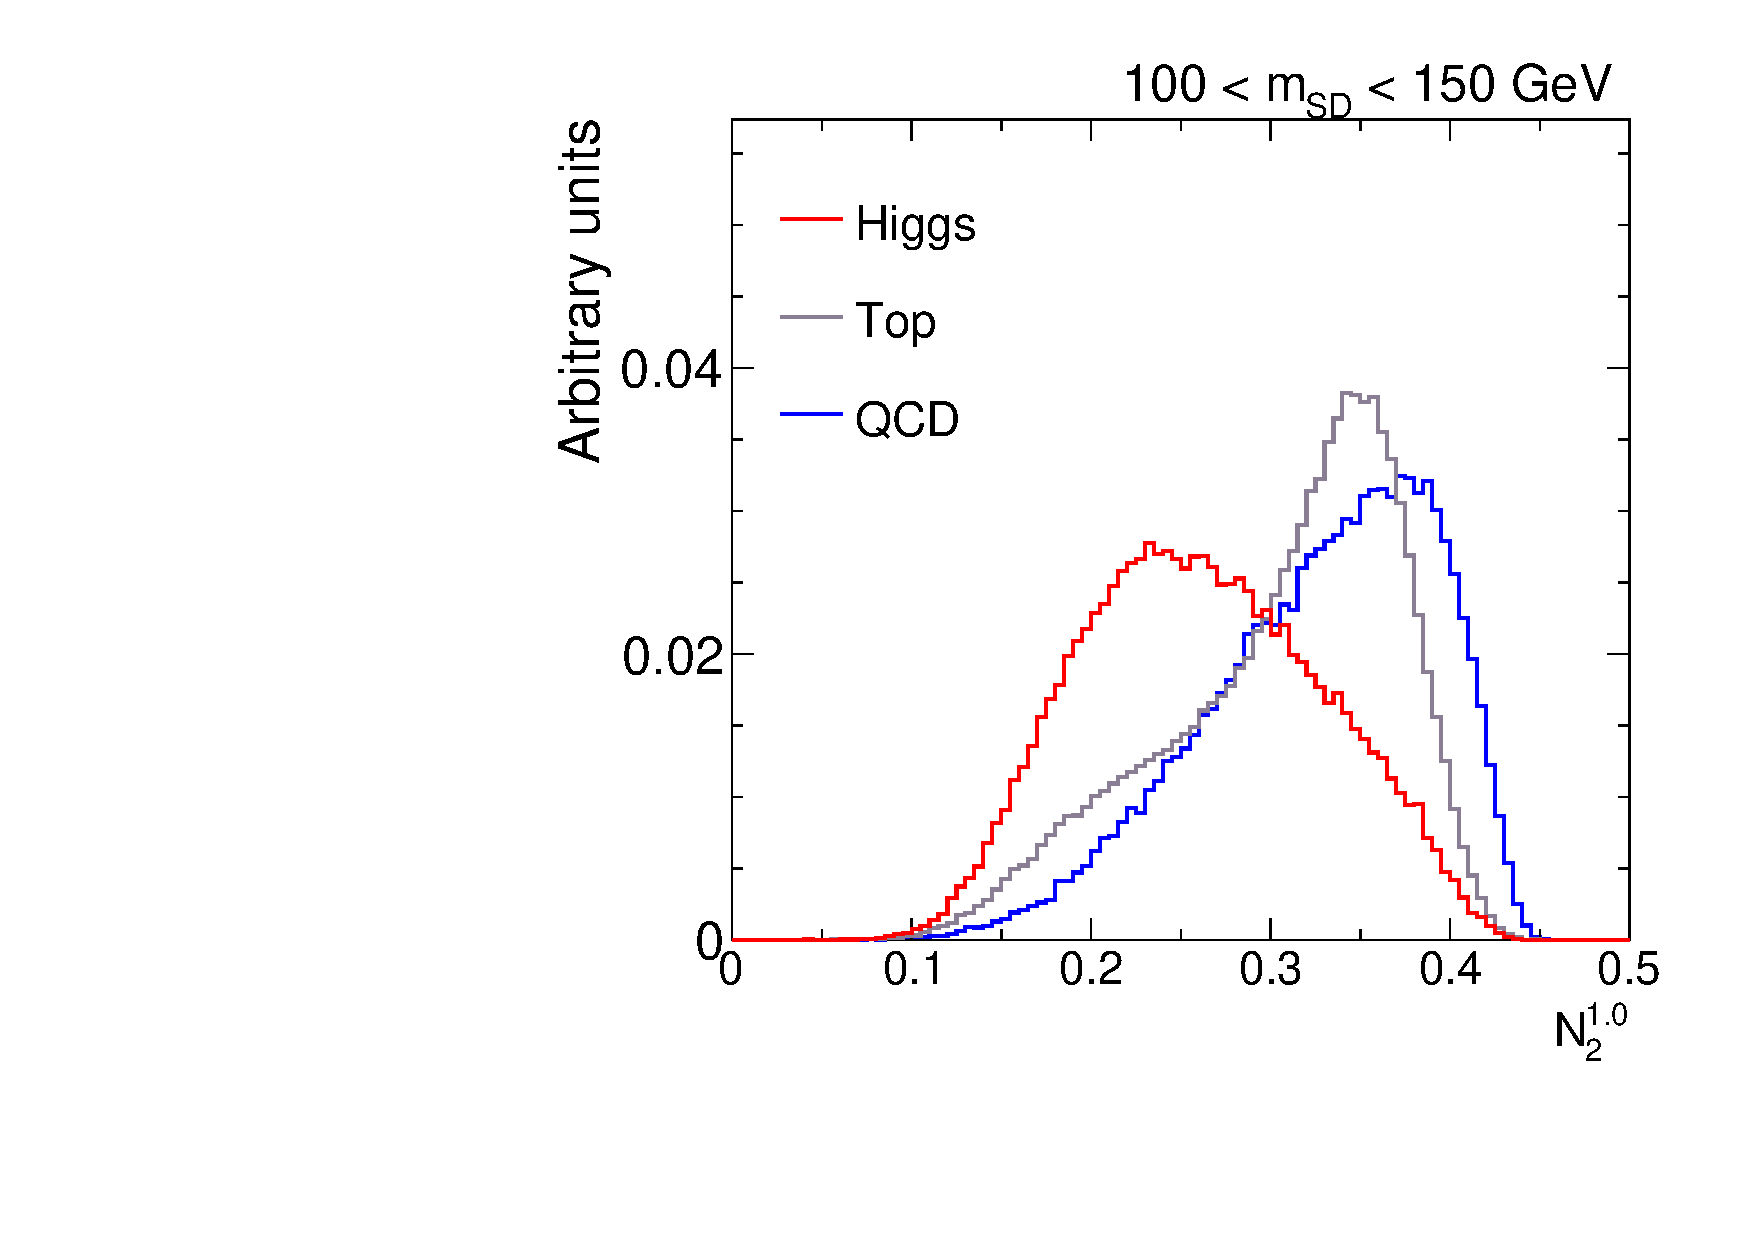
\includegraphics[width=0.475\textwidth]{figures/higgstagging/n2ddt/ddt_N2_10_ns.pdf}
  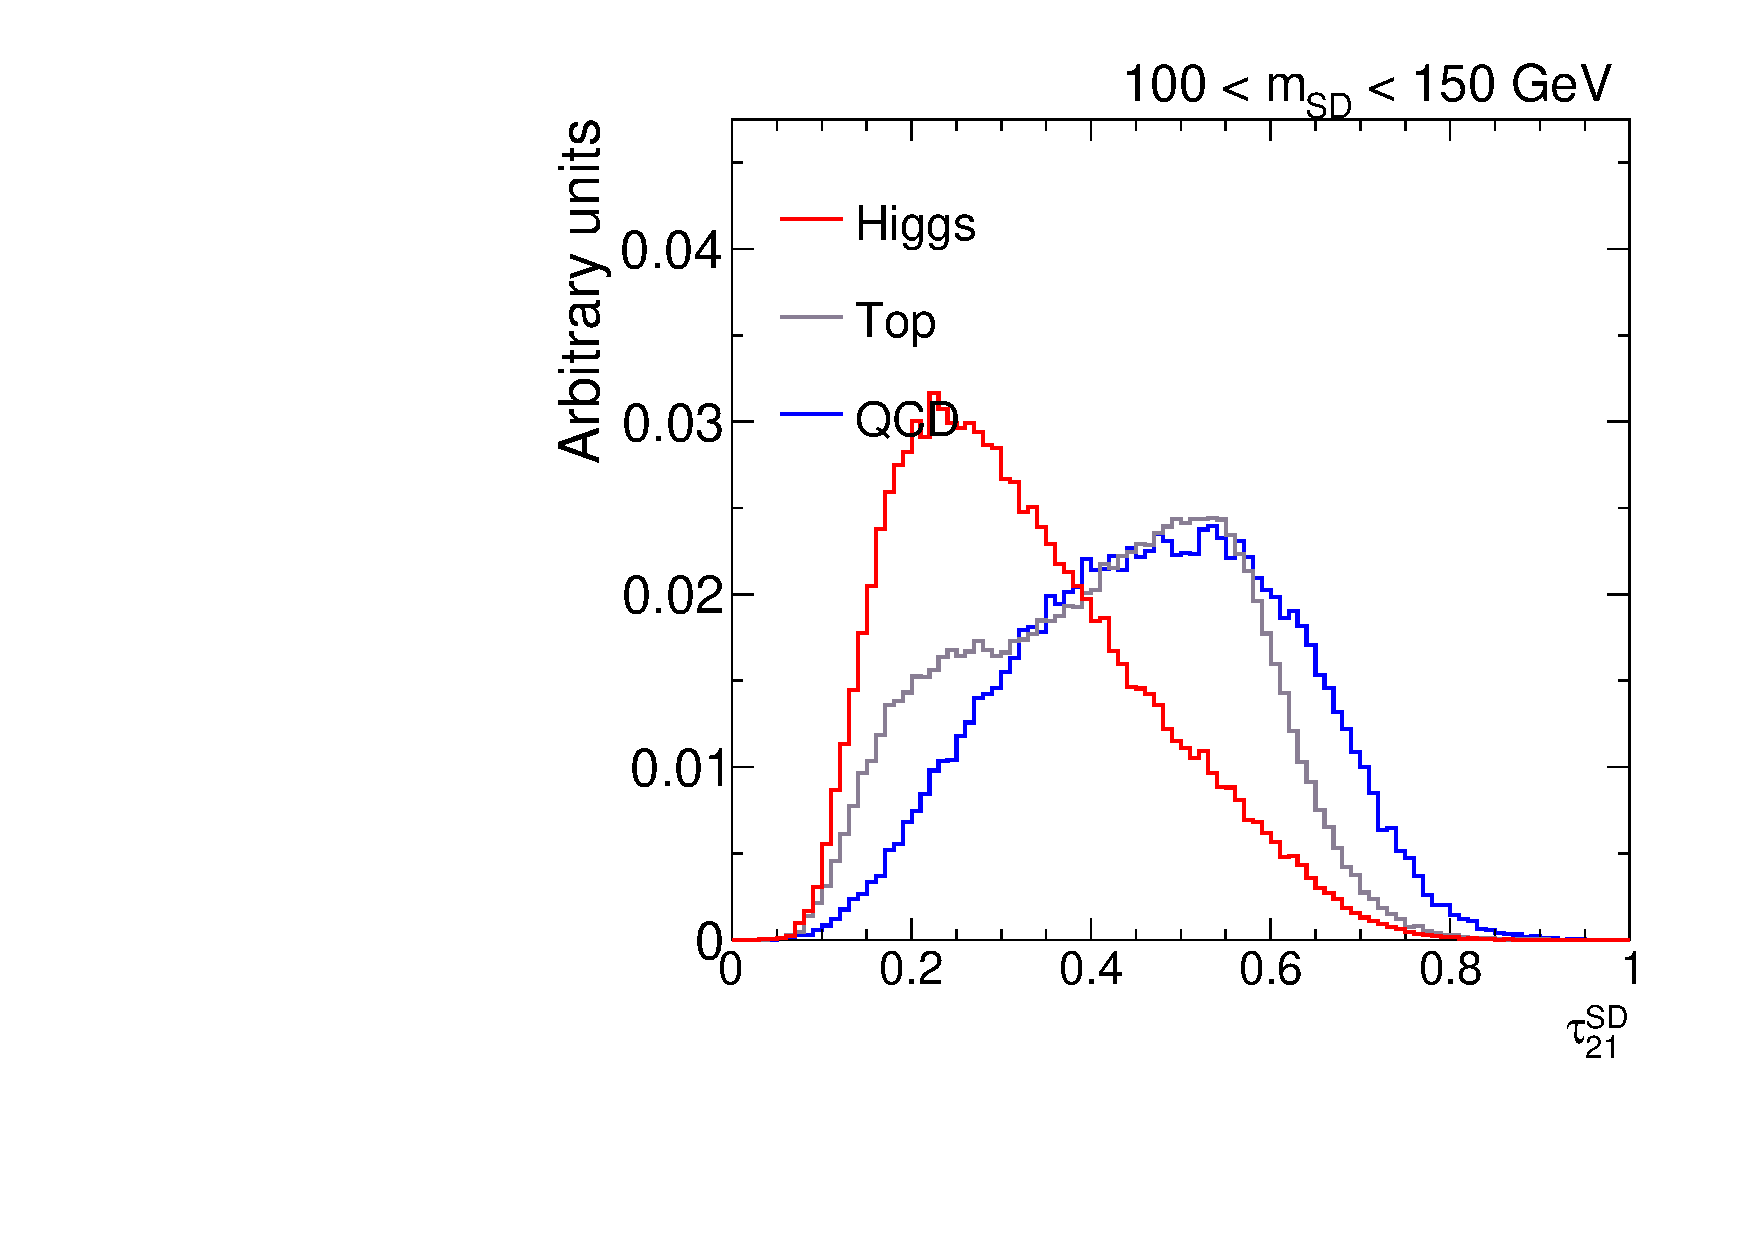
\includegraphics[width=0.475\textwidth]{figures/higgstagging/n2ddt/ddt_tau21SD_ns.pdf}
  \caption{Comparison of $N_2(\beta=1.0)$ and $\tau_{21}^\text{SD}$ for the three main types of jets in the analysis in a window around the true Higgs mass. Event weights are applied that flatten the \pt~spectrum.}
  \label{fig:n2tau21}
\end{figure}


However, as can be seen from Figure~\ref{fig:taggingkinematics}, the mass shape of QCD background fat jets varies significantly with the position of the cut on $N_2$. 

\begin{figure}
  \centering
  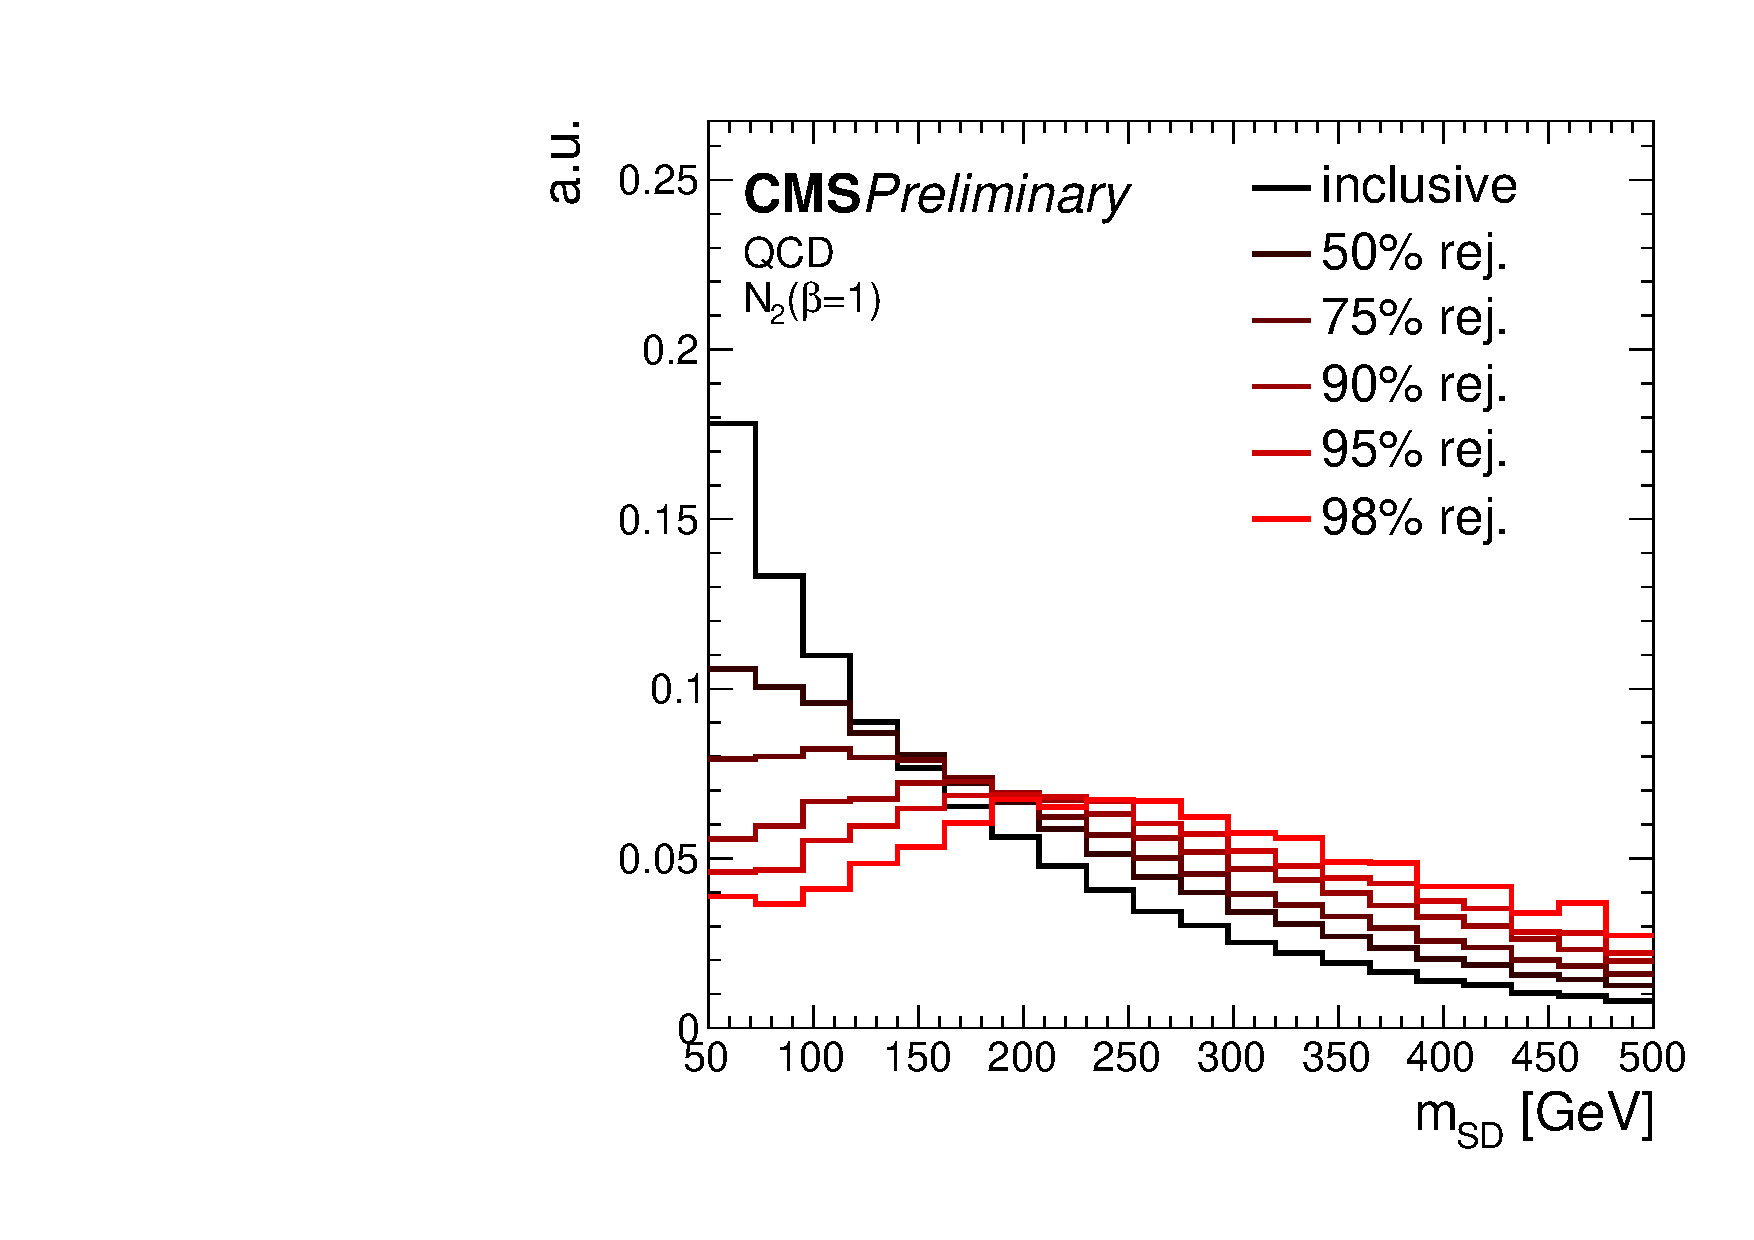
\includegraphics[width=0.475\textwidth]{figures/higgstagging/QCDN2_mSD.pdf}
  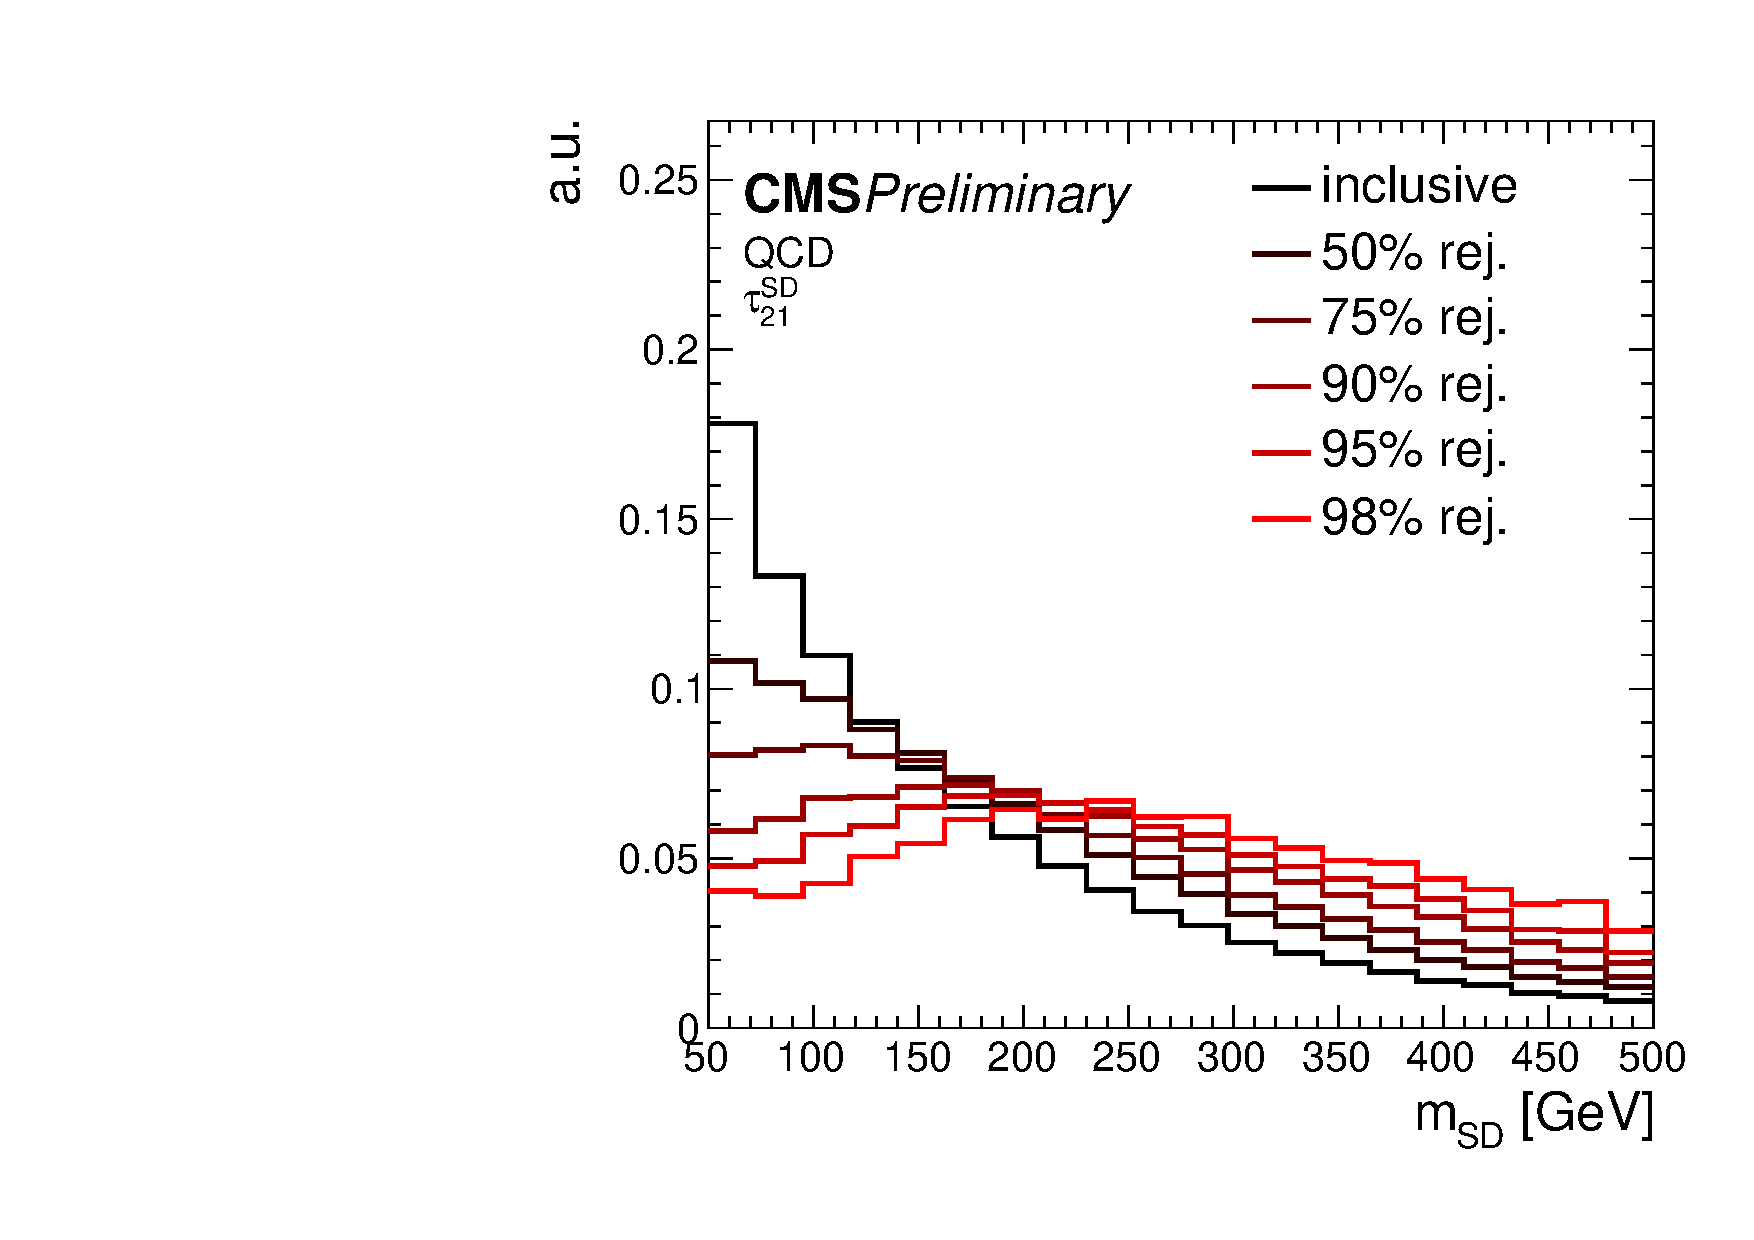
\includegraphics[width=0.475\textwidth]{figures/higgstagging/QCDtau21SD_mSD.pdf}\\
  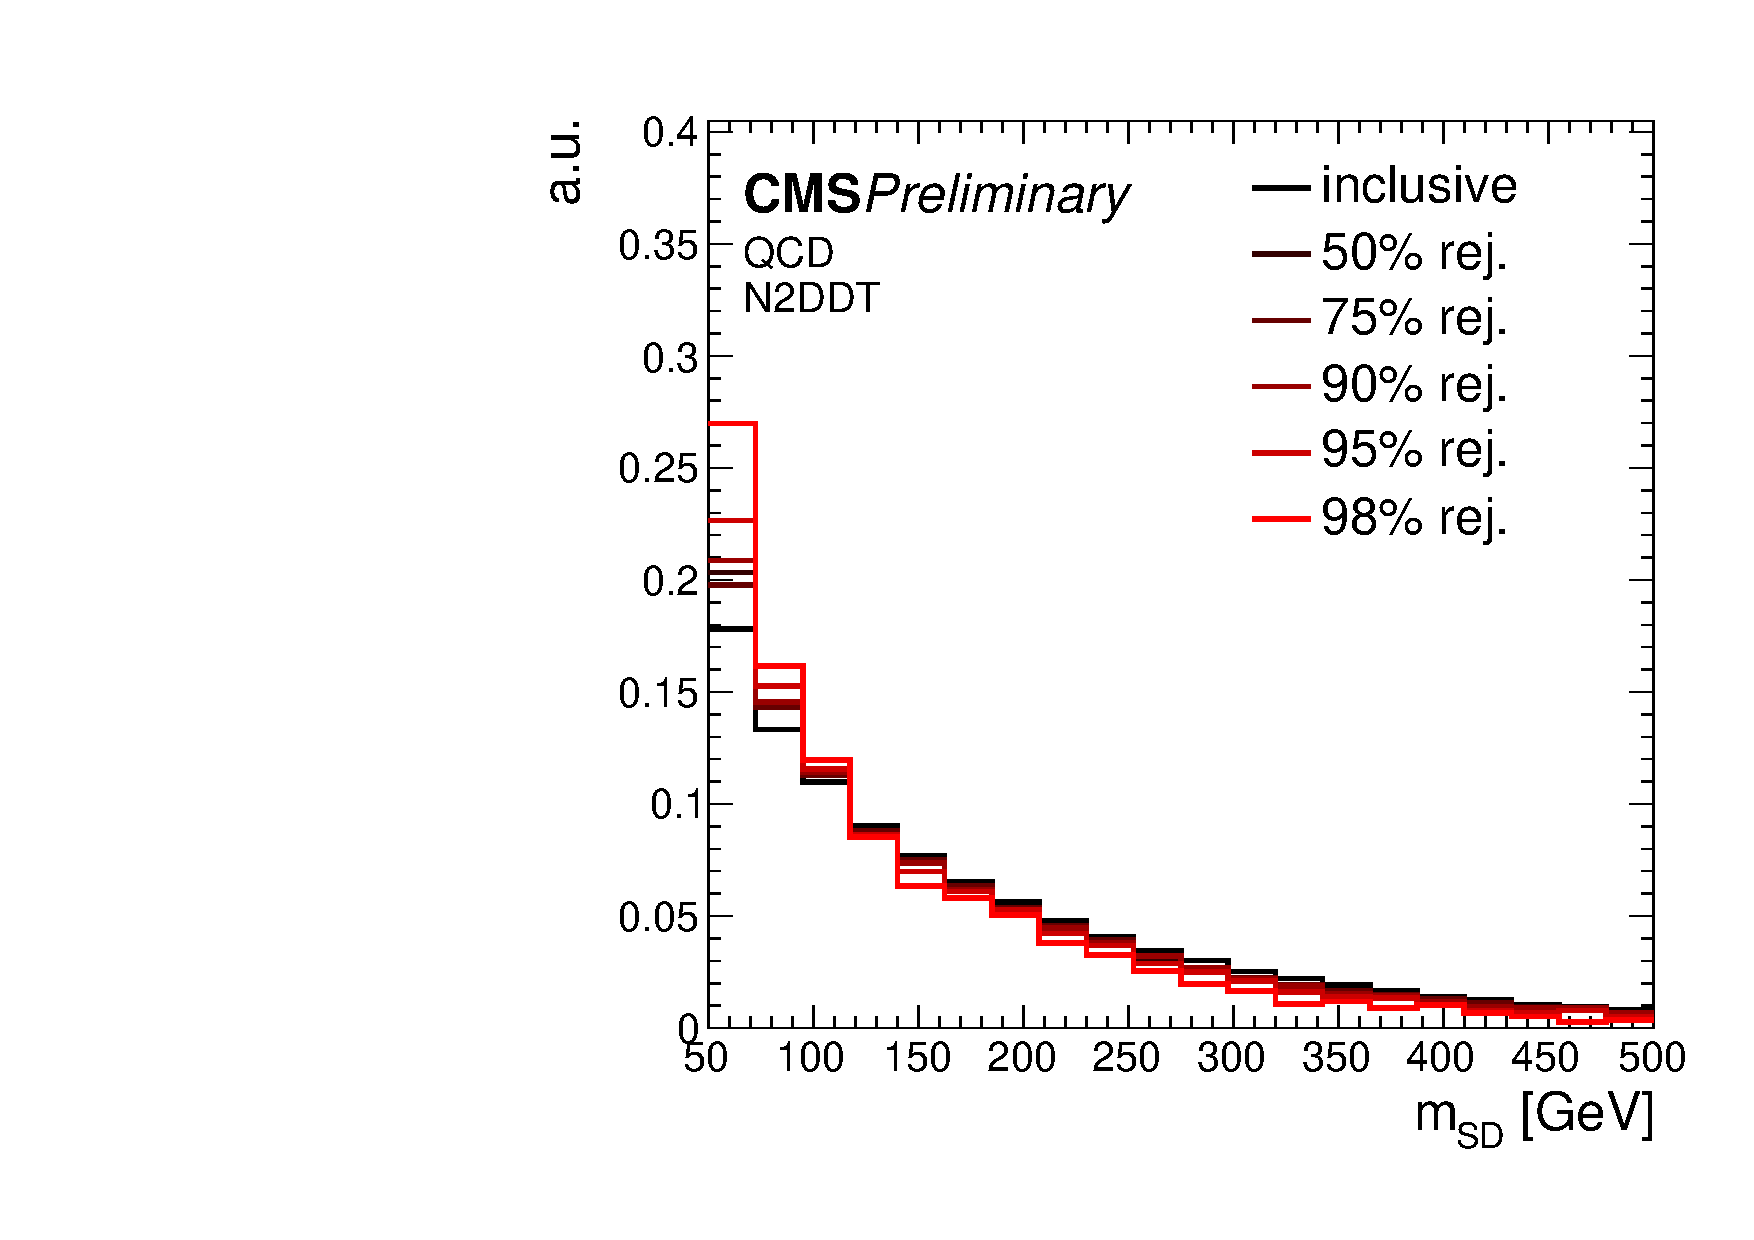
\includegraphics[width=0.475\textwidth]{figures/higgstagging/QCDN2DDT_mSD.pdf}\\
  \caption{Tagging kinematics: shown is the dependence of the soft drop mass on the $N_2$, $\tau_{21}^\text{SD}$, and N2DDT cut. The mass sculpting is pronounced for the variables before decorrelation, while N2DDT shows practically no mass sculpting.}
  \label{fig:taggingkinematics}
\end{figure}


Because we want to preserve a smoothly falling jet mass distribution as a function of \pt, it is natural to determine a substructure variable's stability as a function of the QCD scaling variable $\rho=log(m_{\text{SD}}^2/\pt^2)$.
Since the QCD (quark or gluon-initated) jet mass scales with \pt, decorrelating a given substructure variable as a function of $\rho$ and \pt is a well-bounded procedure.

\begin{figure}
  \centering
  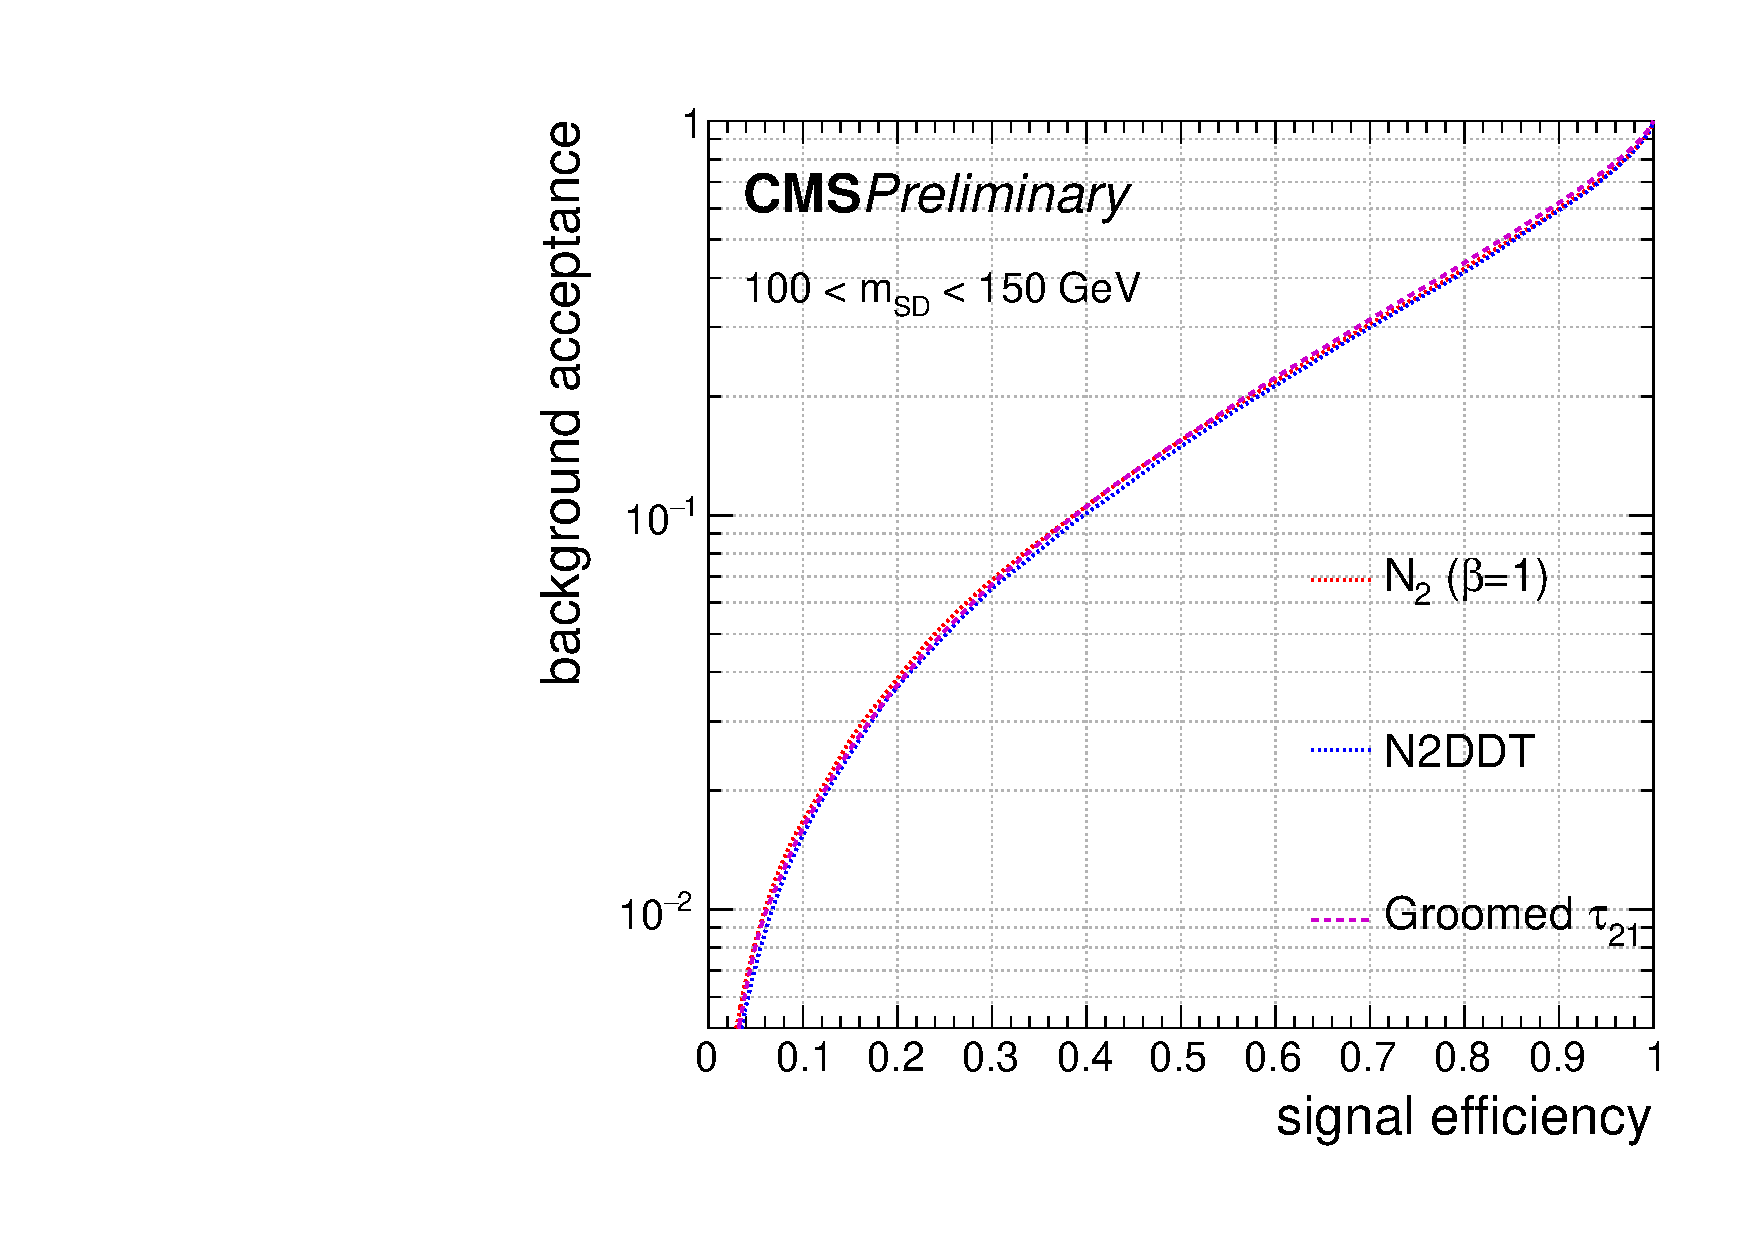
\includegraphics[width=0.475\textwidth]{figures/higgstagging/massCut_roc.pdf}
  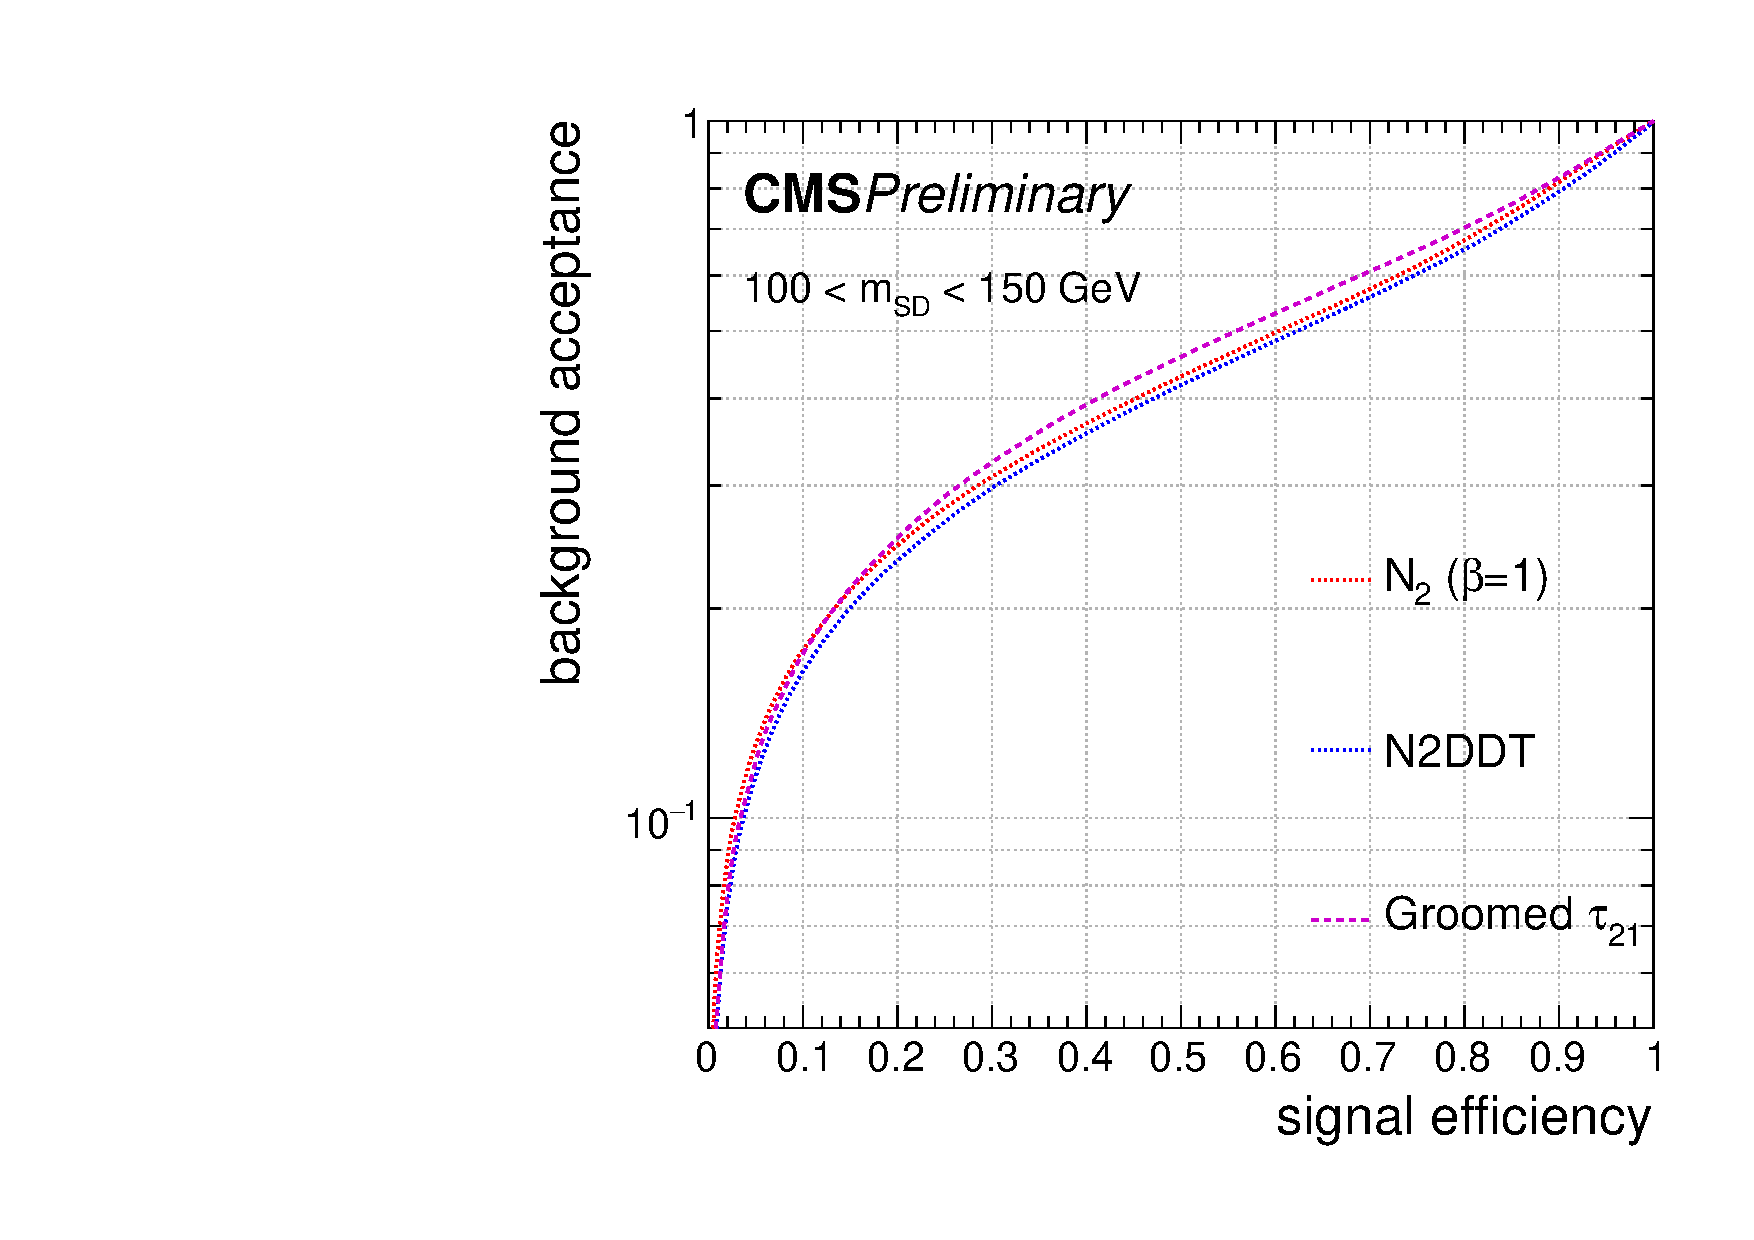
\includegraphics[width=0.475\textwidth]{figures/higgstagging/massCut_roc_top.pdf}\\
  \caption{ROC curves for the $N_2$ and $N$-subjettiness variables. Left: rejection of QCD jets. Right: rejection of top jets. While both $N_2$ and $\tau_{21}$ have similar power to discriminate Higgs jets from QCD jets, $N_2$ does a better job in rejecting fat jets originating from a boosted hadronic top quark decay.}
  \label{fig:n2rocs}
\end{figure}


\begin{figure}
  \centering
  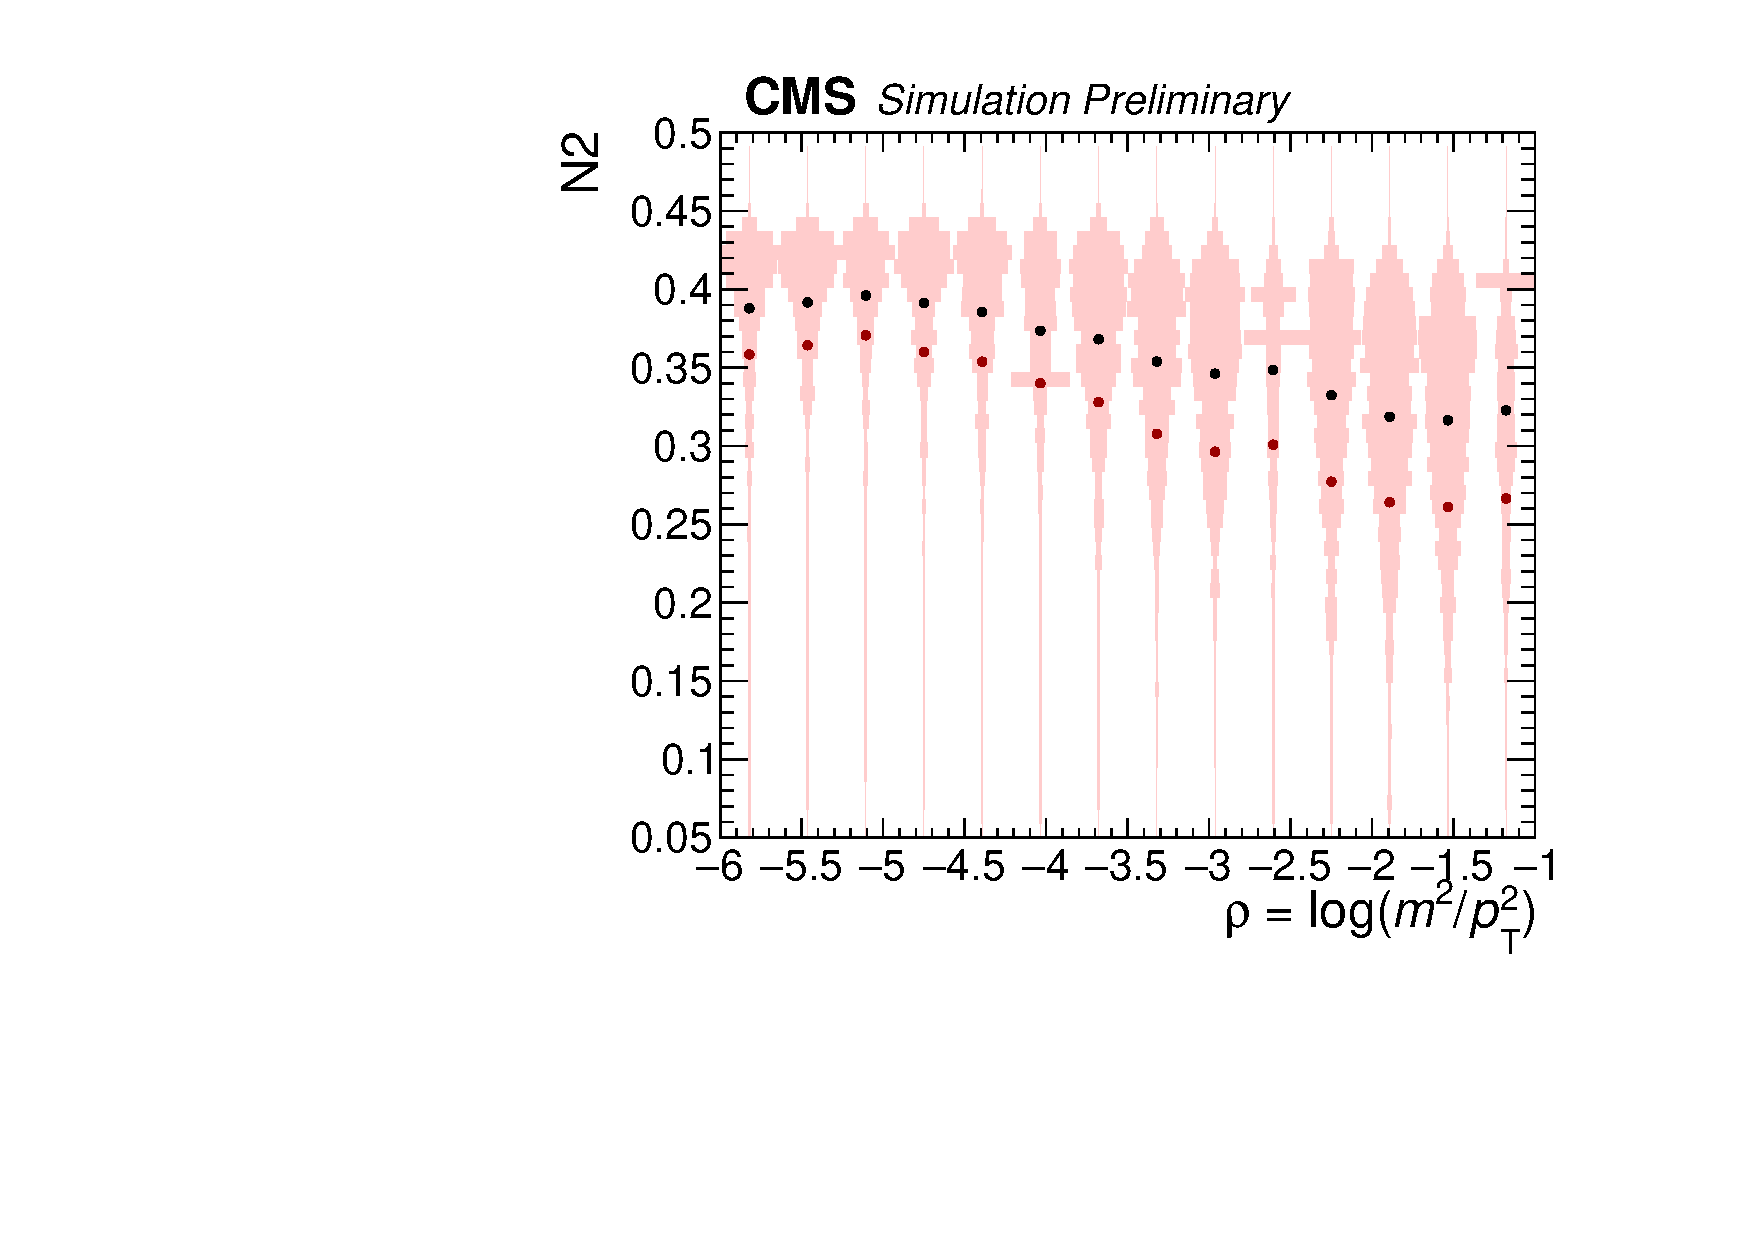
\includegraphics[width=0.38\textwidth]{figures/higgstagging/n2ddt/h2s_n2Vrho0.pdf}\put(-135,25){200-400\GeV}
  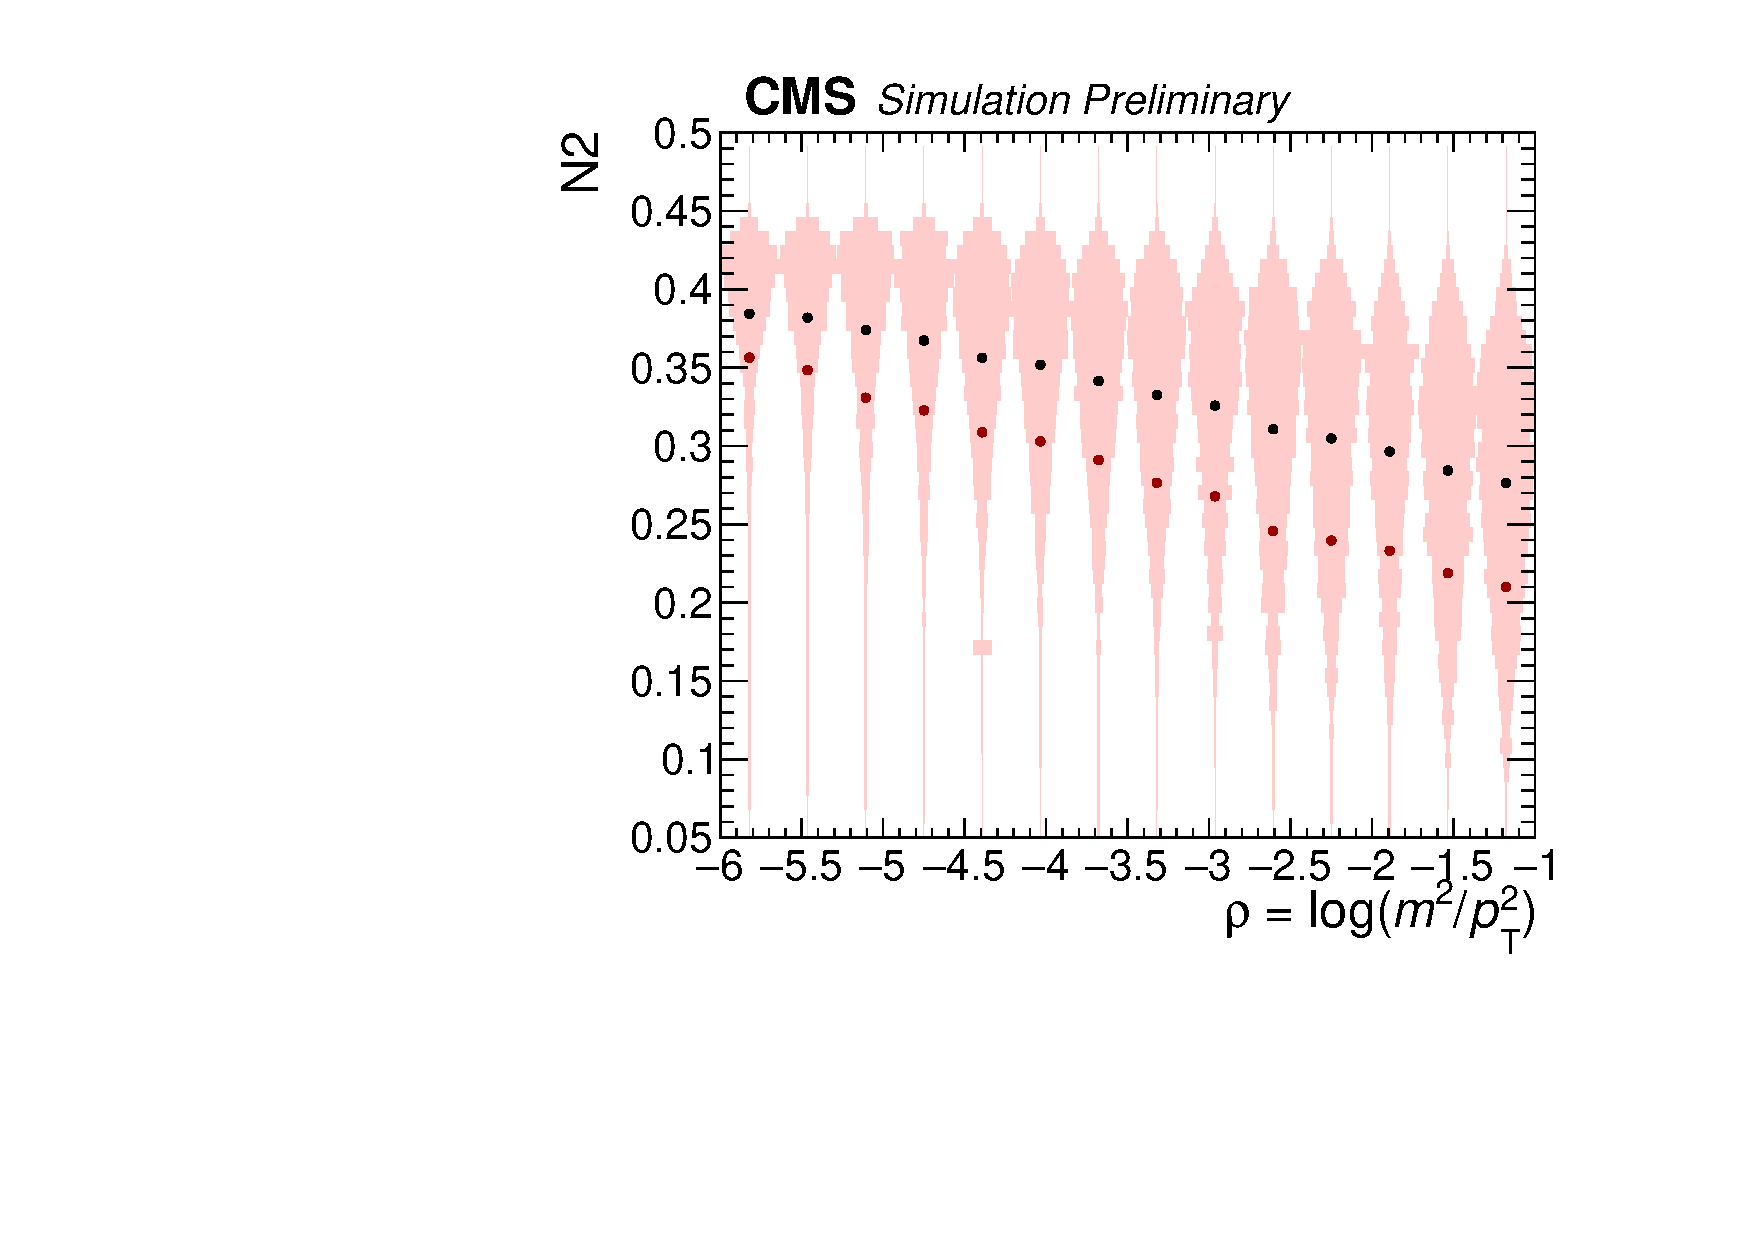
\includegraphics[width=0.38\textwidth]{figures/higgstagging/n2ddt/h2s_n2Vrho1.pdf}\put(-135,25){400-600\GeV}\\
  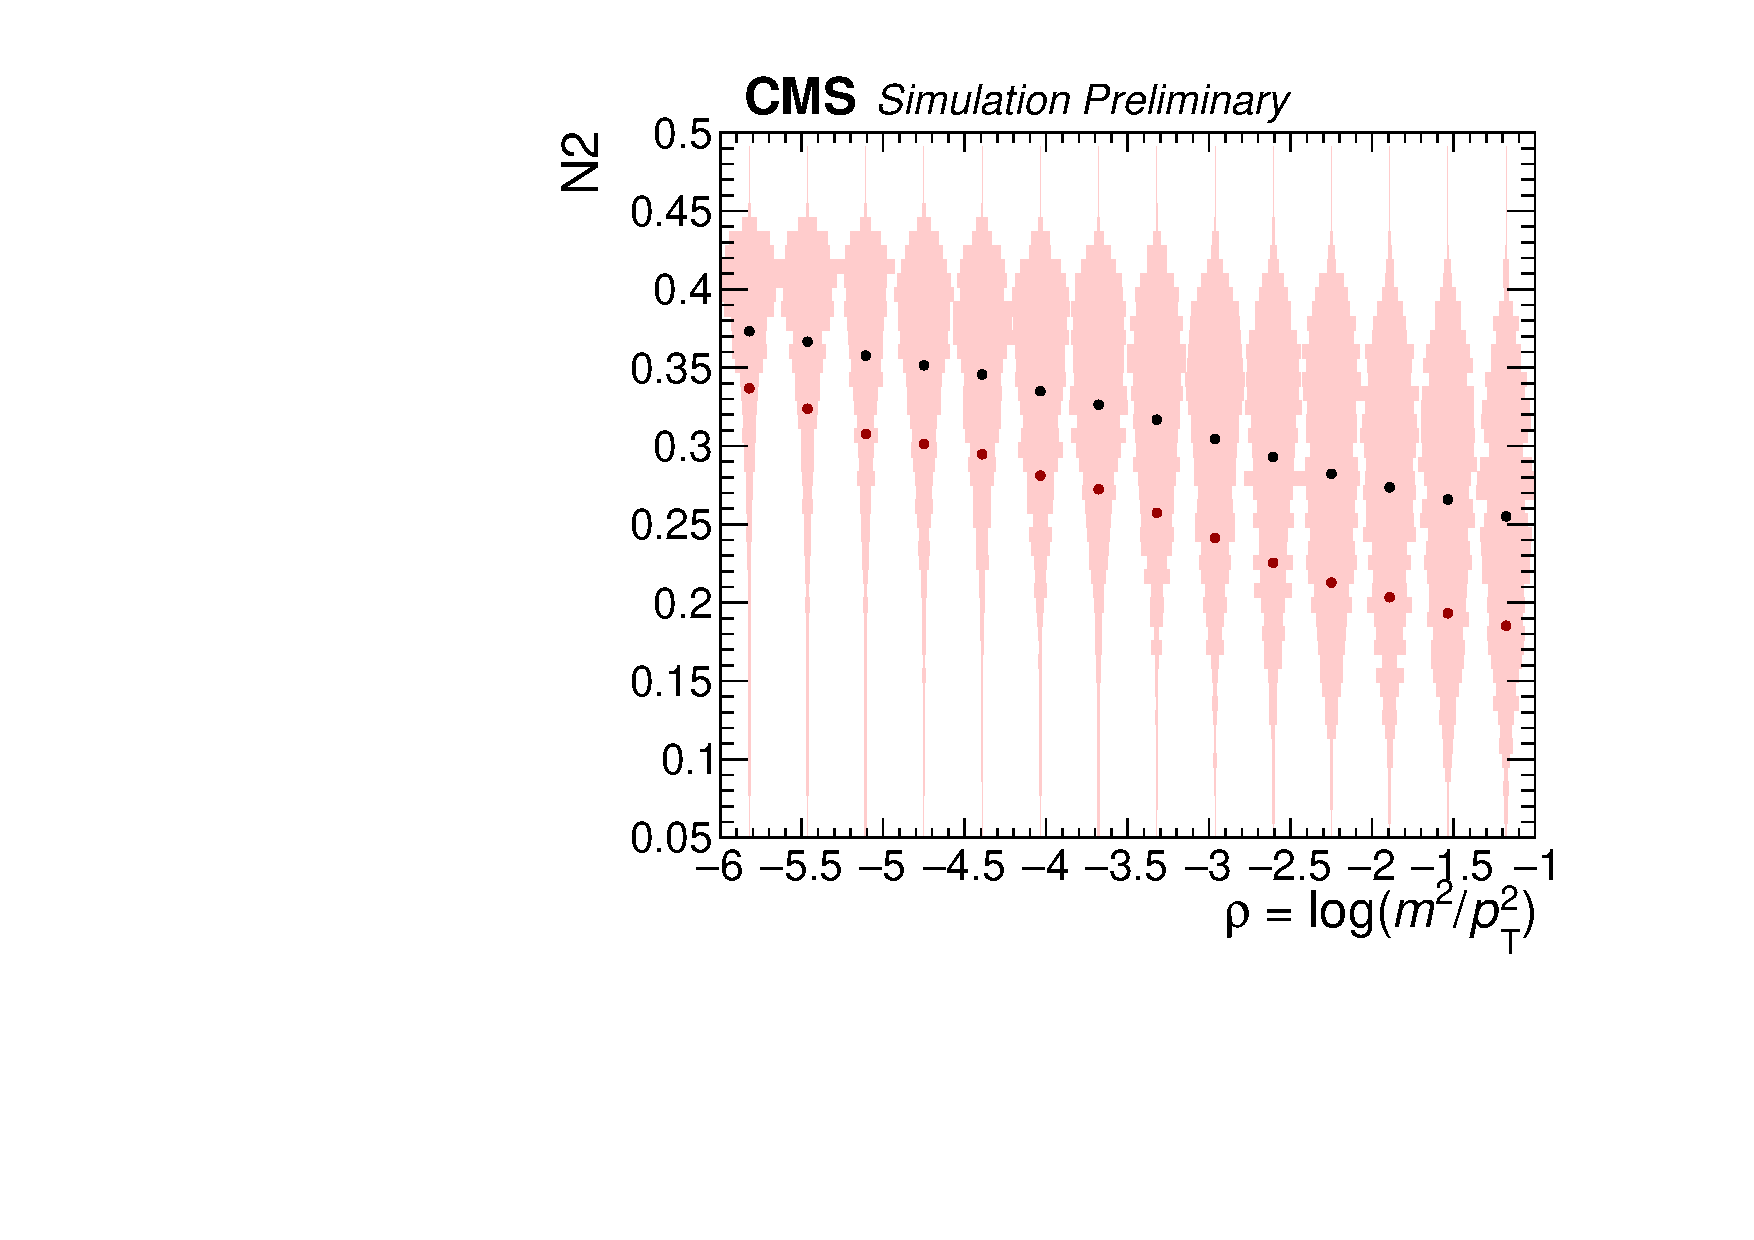
\includegraphics[width=0.38\textwidth]{figures/higgstagging/n2ddt/h2s_n2Vrho2.pdf}\put(-135,25){600-800\GeV}
  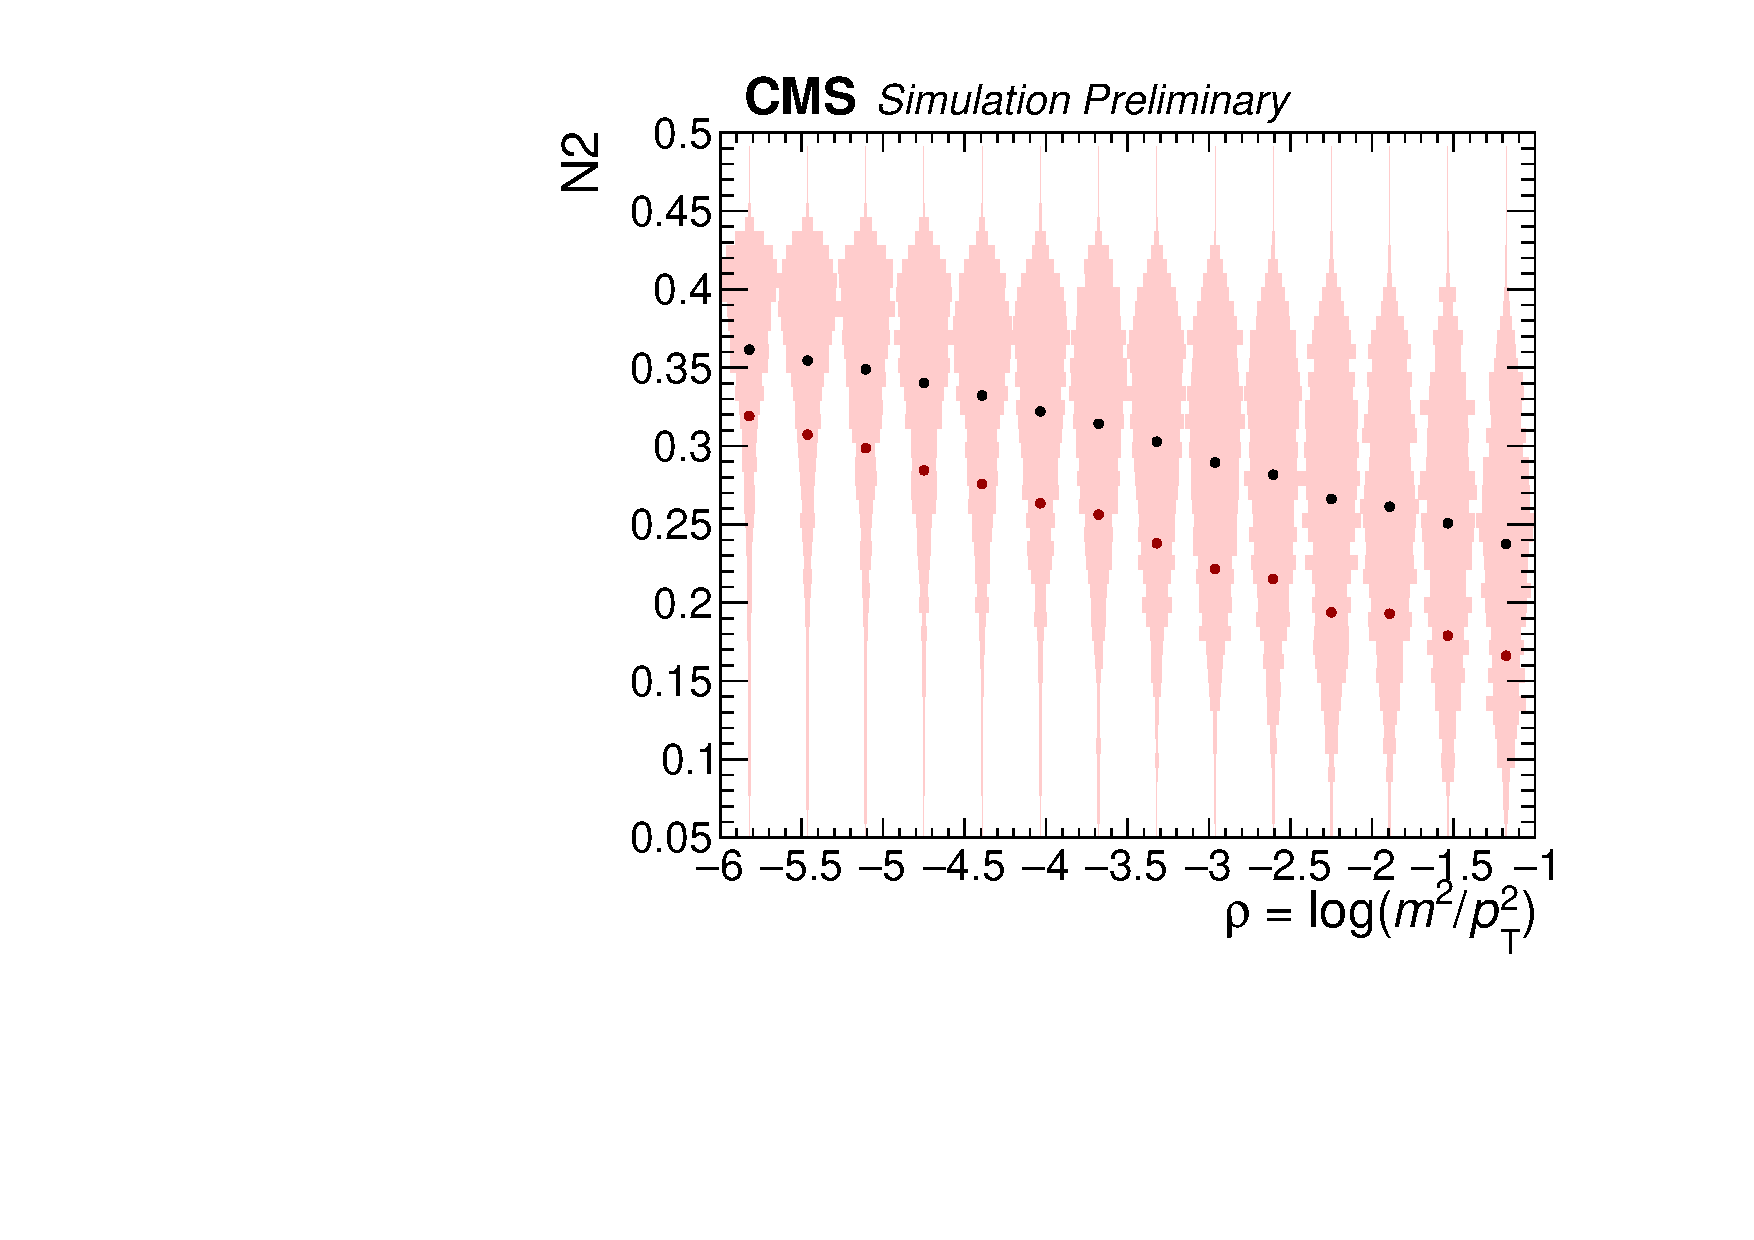
\includegraphics[width=0.38\textwidth]{figures/higgstagging/n2ddt/h2s_n2Vrho3.pdf}\put(-135,25){800-1000\GeV}\\
  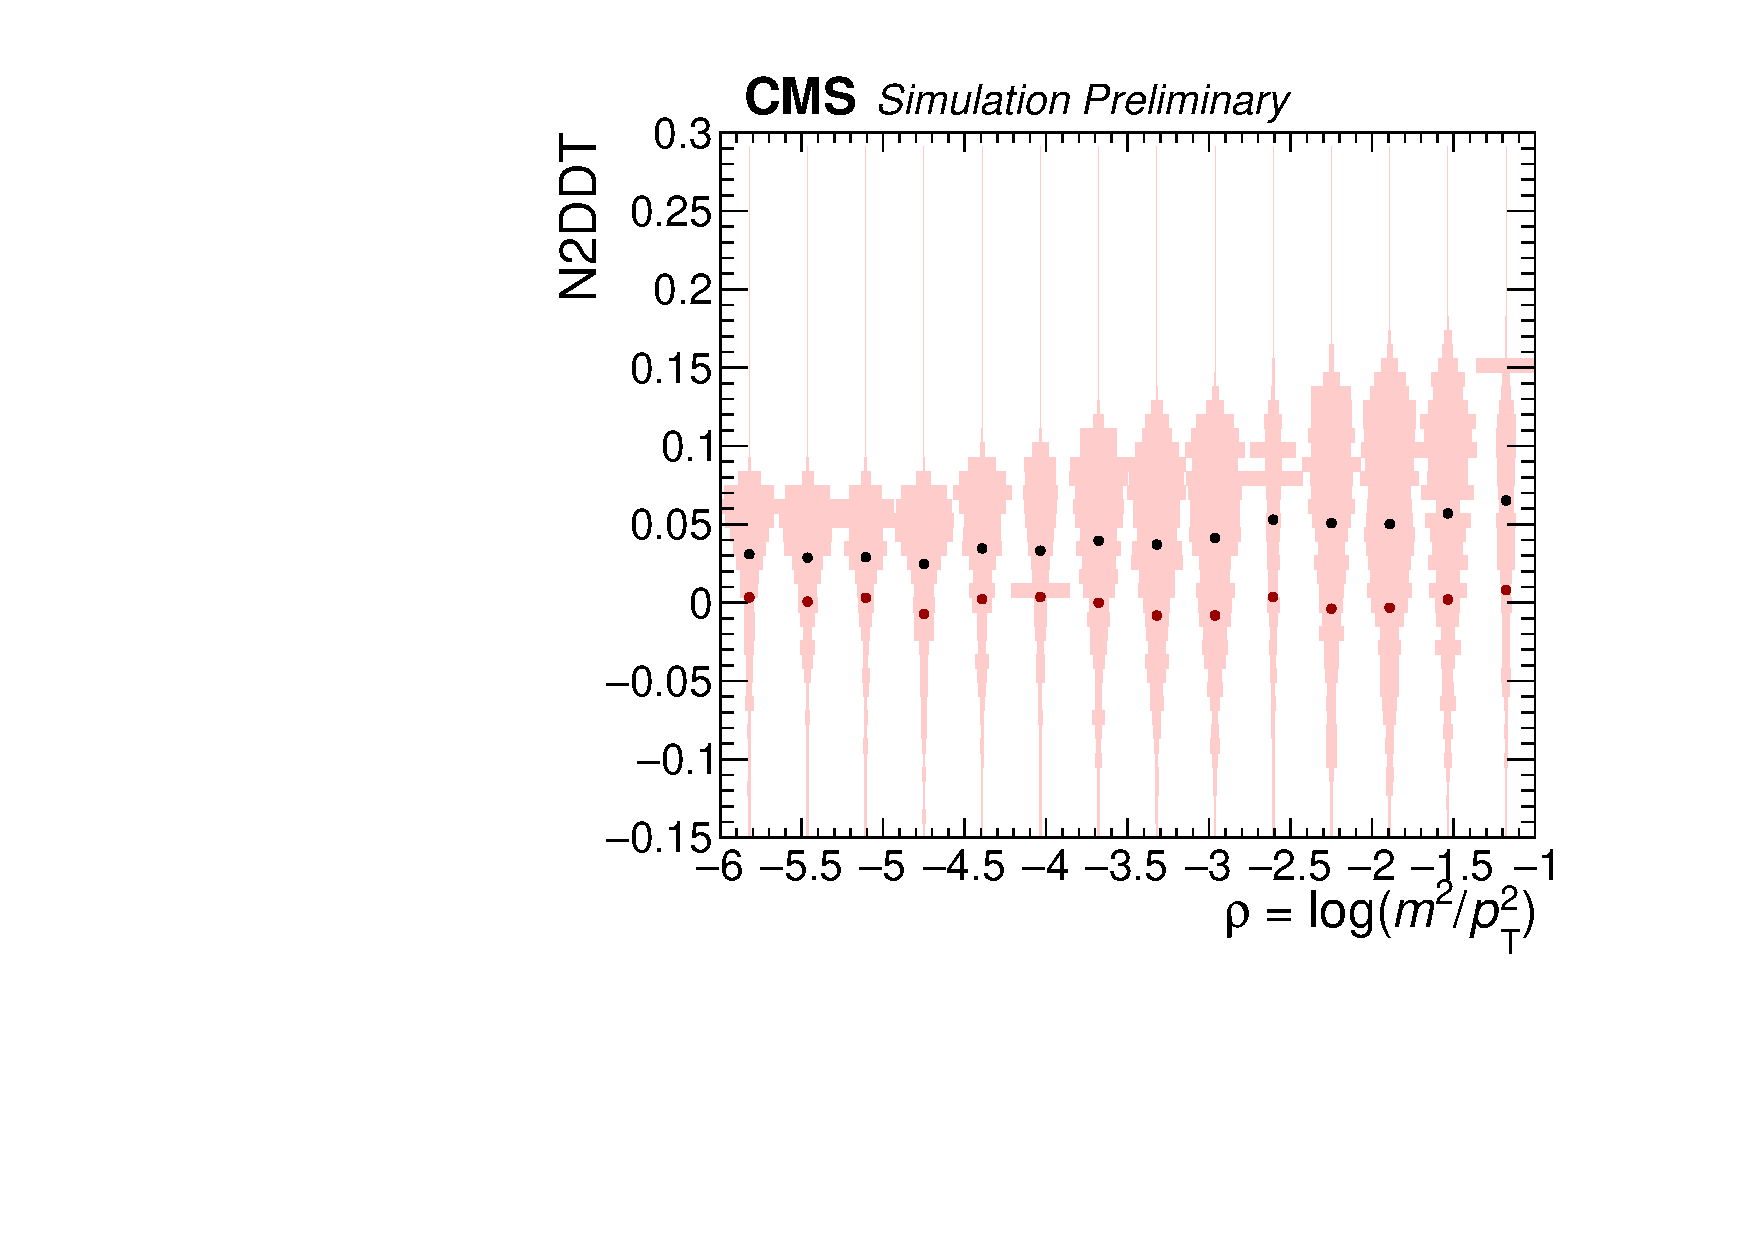
\includegraphics[width=0.38\textwidth]{figures/higgstagging/n2ddt/h2s_n2ddtVrho0.pdf}\put(-135,25){200-400\GeV}
  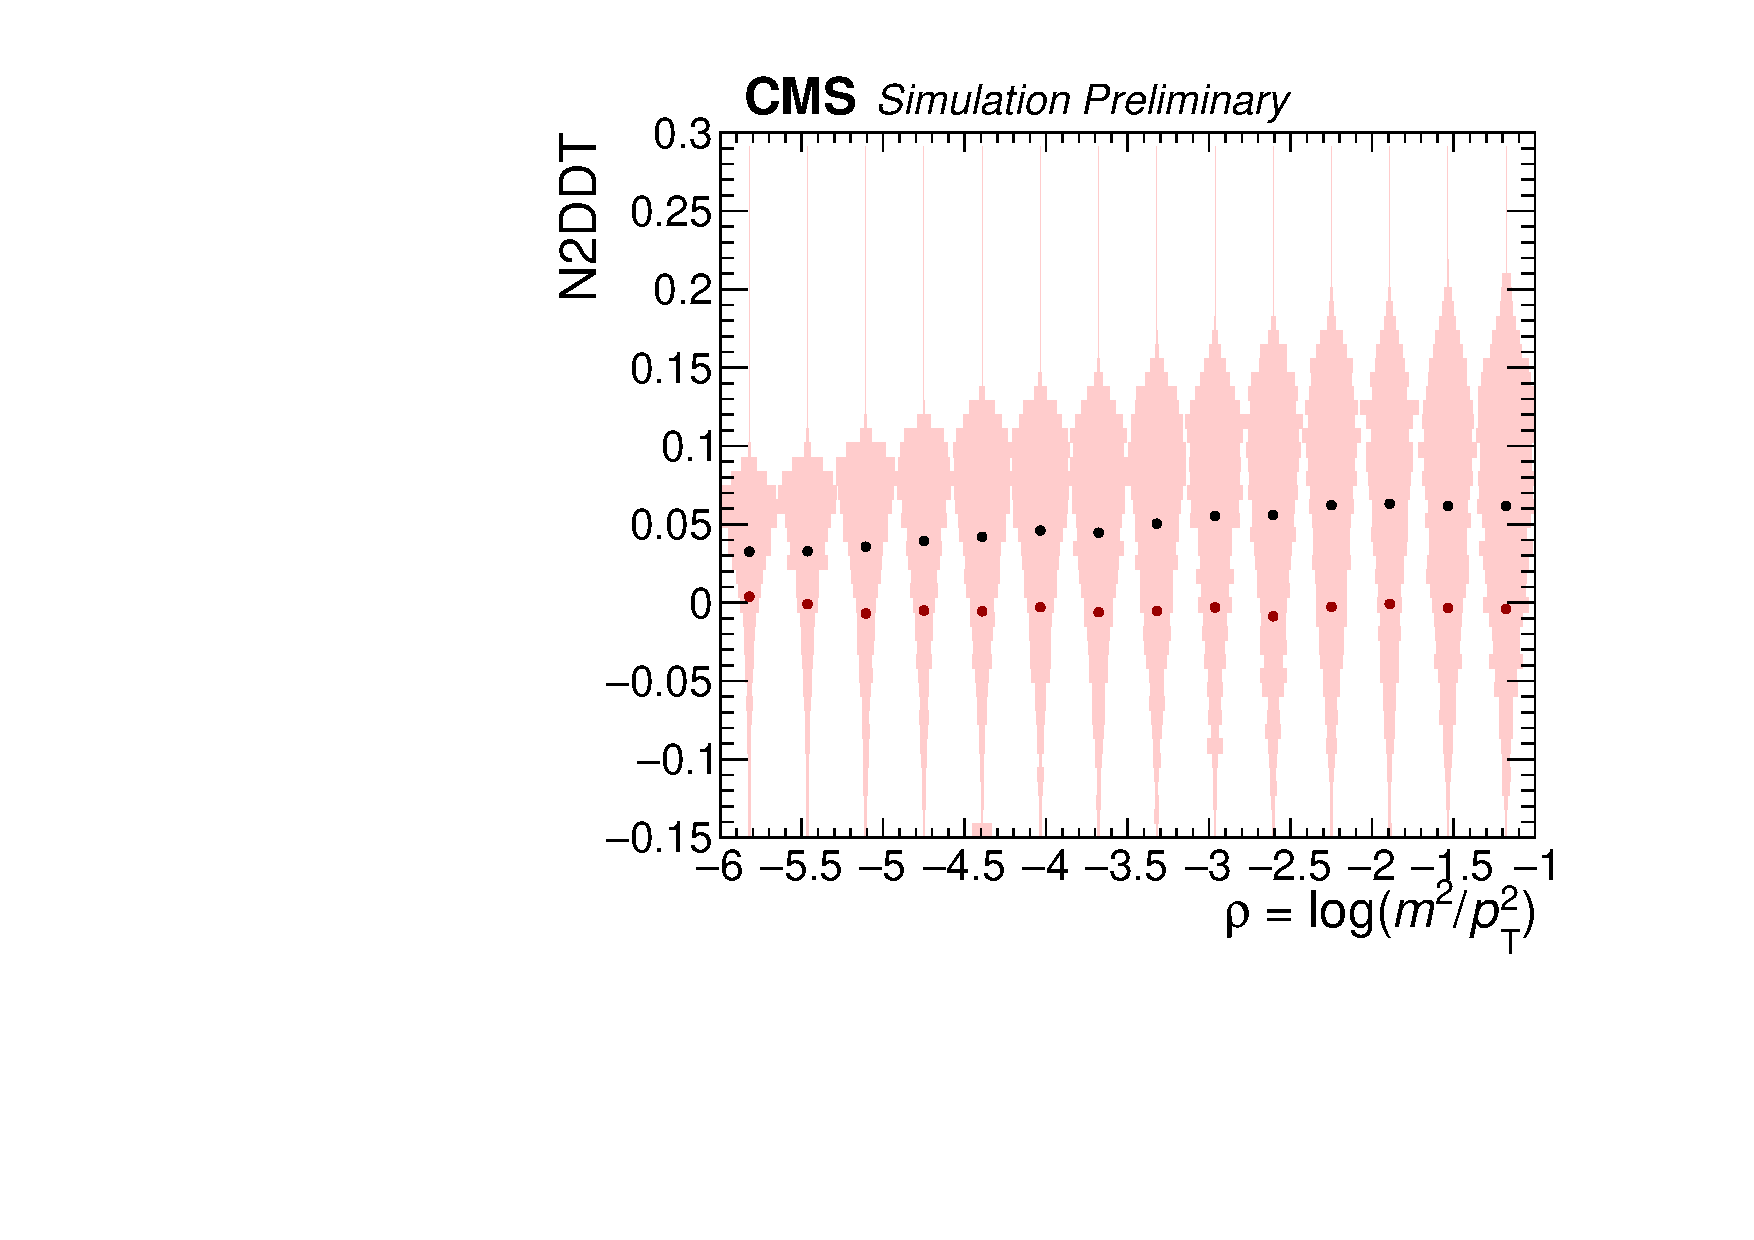
\includegraphics[width=0.38\textwidth]{figures/higgstagging/n2ddt/h2s_n2ddtVrho1.pdf}\put(-135,25){400-600\GeV}\\
  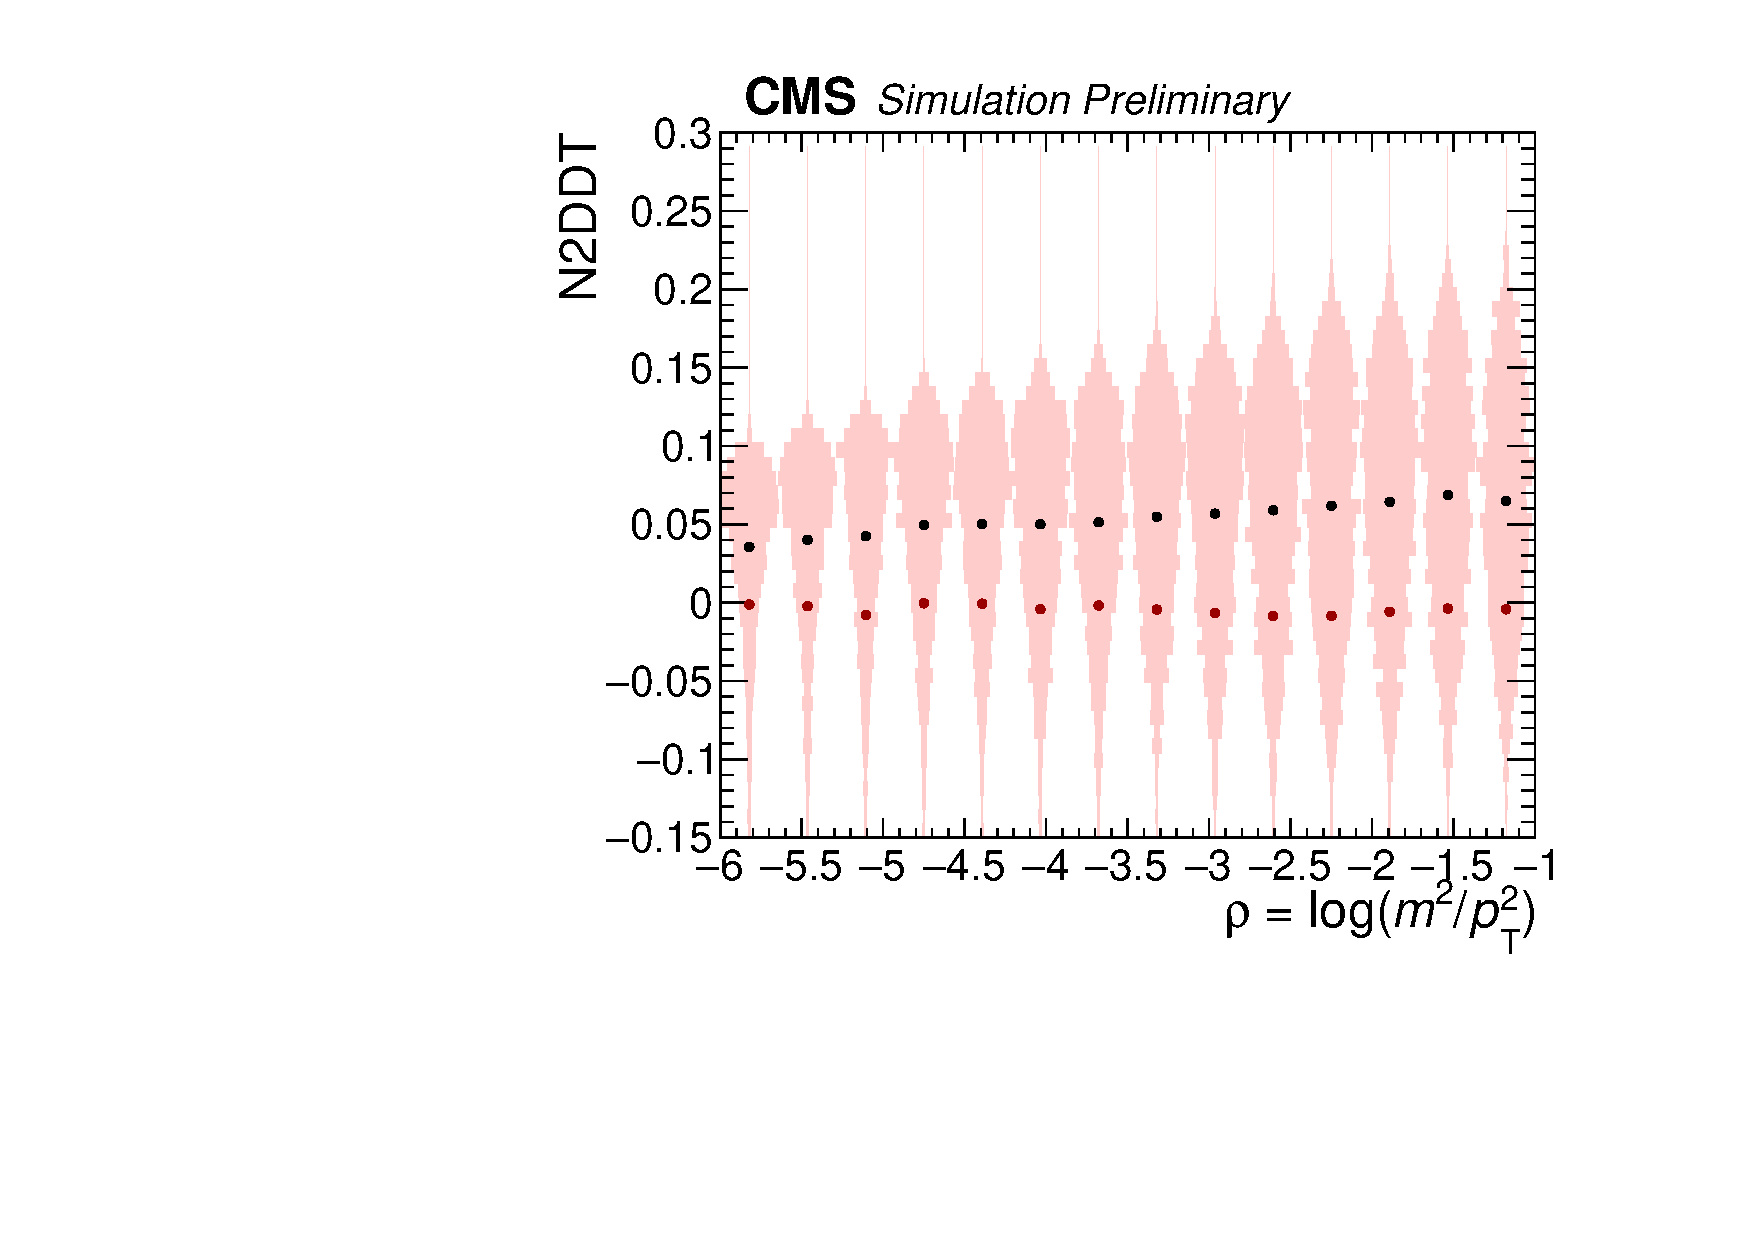
\includegraphics[width=0.38\textwidth]{figures/higgstagging/n2ddt/h2s_n2ddtVrho2.pdf}\put(-135,25){600-800\GeV}
  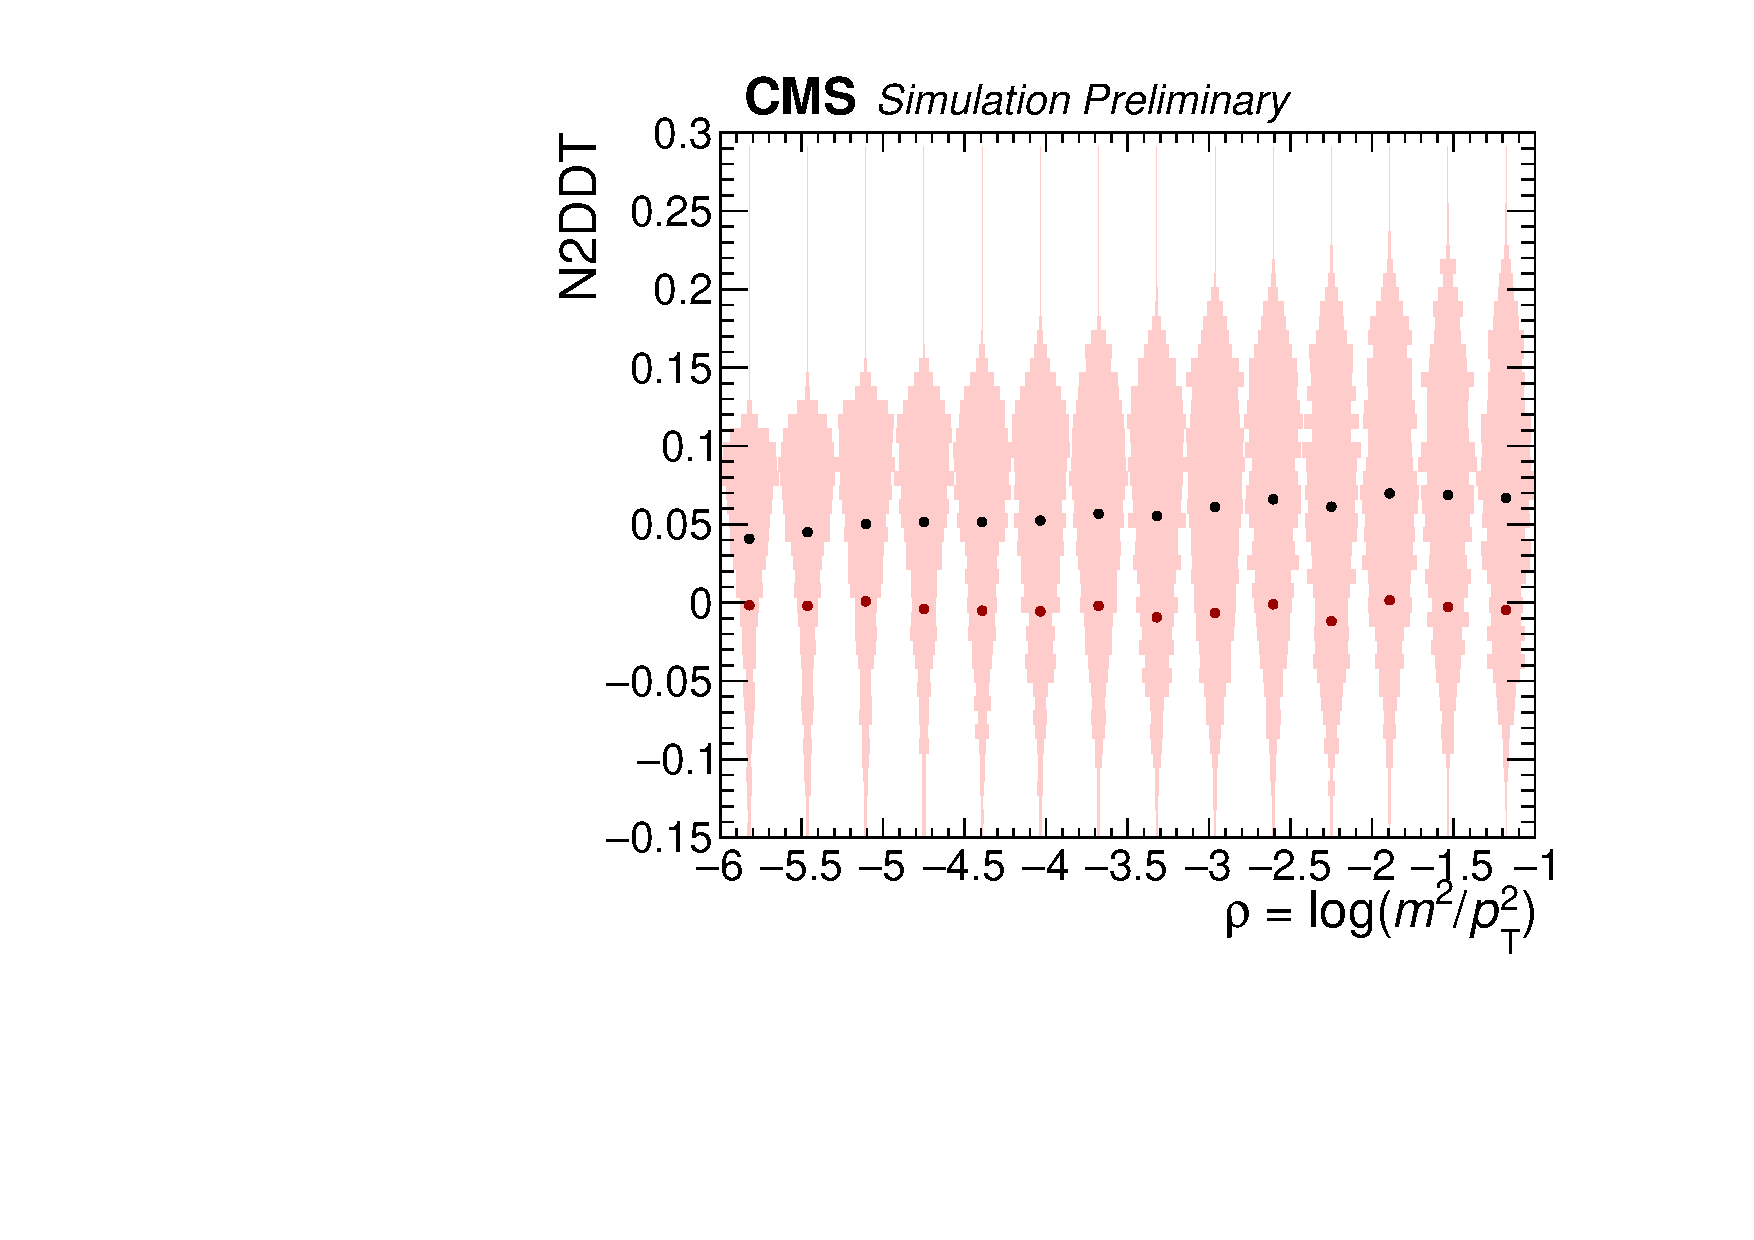
\includegraphics[width=0.38\textwidth]{figures/higgstagging/n2ddt/h2s_n2ddtVrho3.pdf}\put(-135,25){800-1000\GeV}\\
  \caption{Kinematic dependence of $N_2$ and $N_2^\text{DDT}$ as a function of $\rho$ in different \pt bins.}
  \label{fig:violins}
\end{figure}




The decorrelation procedure will be applied at the 20\% background efficiency point, which corresponds to a signal efficiency of roughly 50\%.
This choice of background (or, equivalently, signal) efficiency has been made weighing a good $S/B$ ratio against retaining high enough event yields for the data-driven estimation of the background processes. In particular, going lower in background efficiency brings in large statistical uncertainties on the transfer factors in the simultaneous fit from which we derive upper limits, while a scenario with a significantly higher signal efficiency suffers from large background contaminations degrading the search sensitivity.
The top four plots of Figure~\ref{fig:violins} show the 2D correlations of $\rho$ with $N_2^\text{DDT}$ shown in ``violin'' style for four different \pt bins.
The black dots represent the 50\% background efficiency point for cutting on $N_2^\text{DDT}$ while the red points represent other
the 20\% background efficiency scenario.
%The inflection in the distribution around $\rho = 2$ comes from finite jet size effects which represents a natural limit to the mass of a QCD jet for a given \pt.
Below $\rho = 6$ we enter the non-peturbative regime of the soft drop mass calculation and therefore cut-off the mapping there.
For this analysis a transformation which fixes the background efficiency at 20\% is performed. The efficiency is chosen in agreement with other analyses that use $N_2$ as Higgs-tagging variable (usually around 25\%), tuned to optimize the sensitivity to the mono-Higgs signal.  
The 2D map in $\{\rho,\pt\}$ space which transforms $N_2 \rightarrow N_2^\text{DDT}$ is shown in Fig.~\ref{fig:transmap_20percent}.
Therefore, the transformation is defined as:
\begin{equation}
N_2^\text{DDT} = N_2 - N_2(\text{cut at 20\%})
\end{equation}

\begin{figure}
  \centering
  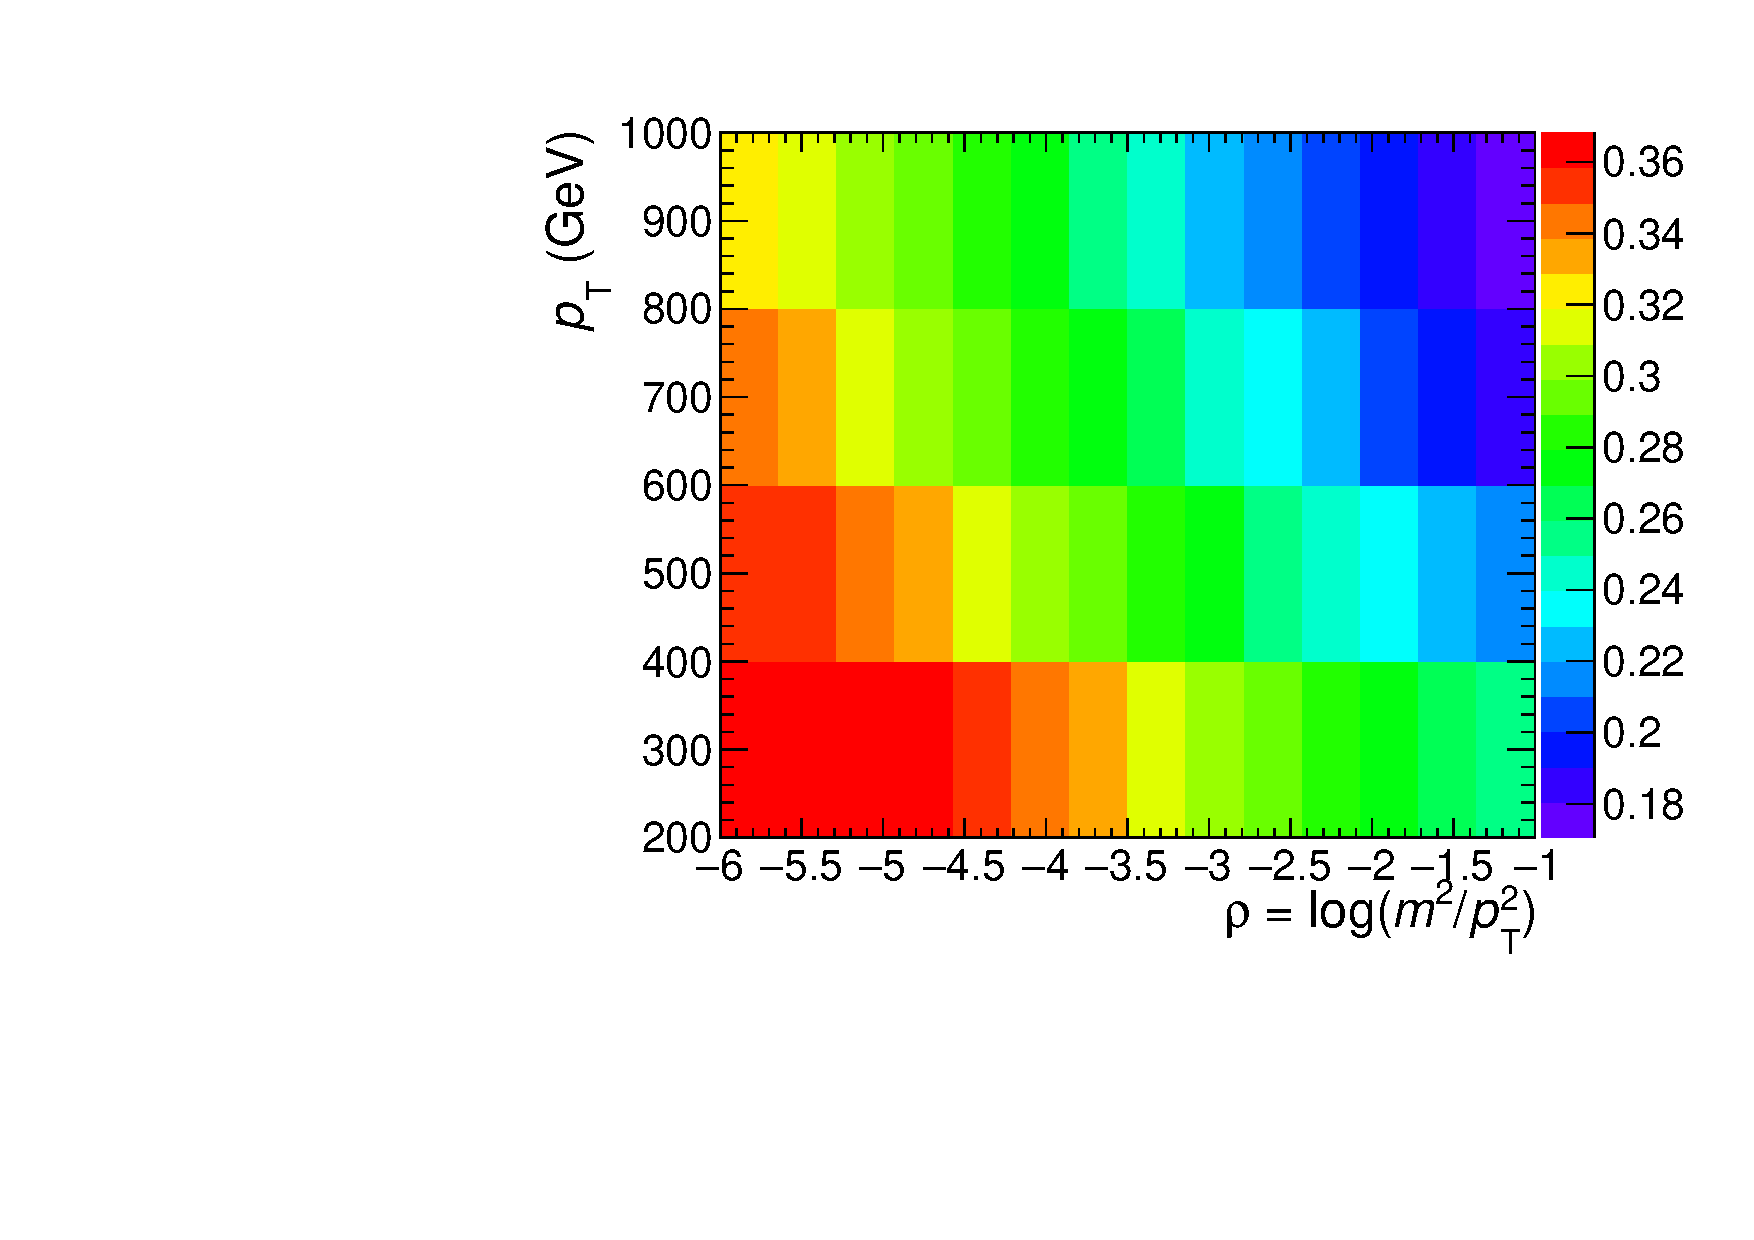
\includegraphics[width=0.475\textwidth]{figures/higgstagging/n2ddt/h2ddt.pdf}
  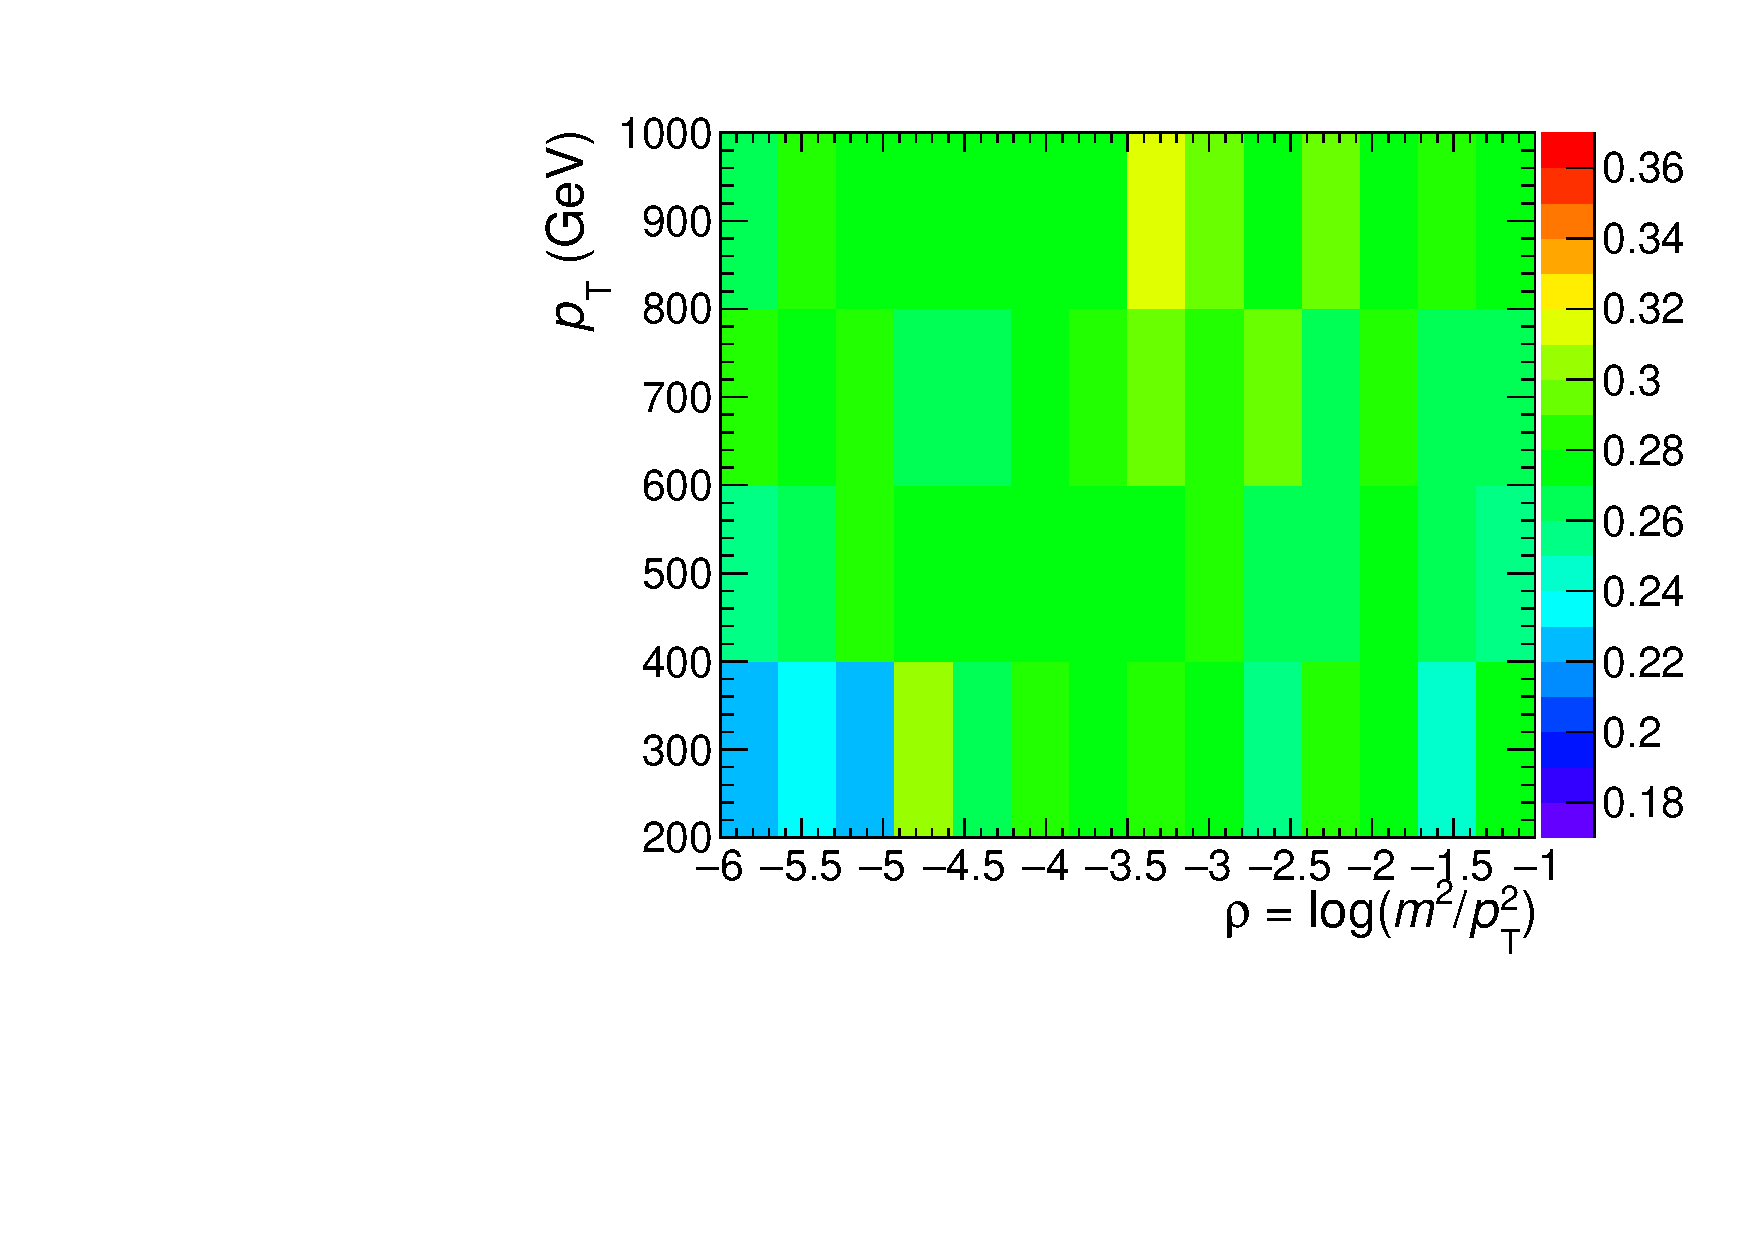
\includegraphics[width=0.475\textwidth]{figures/higgstagging/n2ddt/h2_rhoVpt_pafa.pdf}\\
  \caption{Left: transformation map of $N_2\rightarrow N_2^{\text{DDT}}$. Right: the $z$-axis gives the ``pass-over-fail'' ratio when cutting on $N_2^\text{DDT}<0$. By construction, this ratio is equal to $0.2/0.8\sim0.25$. This is found across all bins in $\rho$ and $\pt$.}
  \label{fig:transmap_20percent}
\end{figure}

The ``pass-over-fail'' in QCD background is also shown in Fig.~\ref{fig:transmap_20percent}. We observe tagging (in)efficiencies that are flat across the entire phase space. 


Once a cut on this variable is applied to both MC and data, different residual tagging efficiencies have to be accounted for by means of a scale factor. This scale factor is measured in semileptonic \ttbar events, where the top quark is not fully merged, but one is instead left with a fat jet stemming from a hadronically decaying boosted W boson~\cite{monoH}.


%%%
%In order to extract the W-tagging scale factors, the W-tagging efficiency of a pure W-jet sample must be estimated in data and simulation. This is done by validating the shapes of the real, merged Ws and the pure combinatorial background for the pass and fail W-tagged events in the \ttbar simulated sample. The \ttbar sample is divided into the combinatorial background and the real, merged Ws at generator level, matching the CA15 jet in a cone of $\Delta R <1.5$ of a hadroncially decaying W boson and the daughter quarks within a cone of $\Delta R <1.5$ of the jet axis. The fit functions used for the matched and unmatched events are:

%$$f_{pass}^{sig} = Frac \cdot F_{Gaus}(m_{j}) + F_{ErfExp}(m_{j})$$
%$$f_{fail}^{sig} = Frac \cdot F_{Gaus}(m_{j}) + F_{Exp}(m_{j})$$


%This measurement has been performed in~\cite{N2DDTMichael}. We refer the reader to there for more details concerning the selection and the fit and just show the resulting distributions in the pass/fail bin in Fig.~\ref{fig:TotalFits}. The final scale factor, given by the ratio of integrals of the Gaussian pass and fail curves for MC and data, is provided in Table~\ref{tab:ScaleFactors}. The numerical results of the fit are given in Tables~\ref{tab:ScaleFactors},\ref{tab:FitParameters} and turns out to be consistent with 1. The systematic uncertainty comes from employing a different analytic function (Double Crystal Ball) for describing the pass sample. 

%\begin{table}[htbH]
%  \begin{center}
%    \topcaption{Data-to-simulation scale factors for two different $N_{2}^{DDT}$ transformations.}
%    \begin{tabular}{l|c}
%      \hline
%      \hline
%      Variable & Scale Factor \\
%      \hline
%      $N_{2}^{DDT}$(CA15)     & $0.97\pm0.06$(stat)$\pm0.04$(sys)  \\
%      \hline
%      \hline
%    \end{tabular}
%    \label{tab:ScaleFactors}
%  \end{center}
%\end{table}

%\begin{table}[htbH]
%  \begin{center}
%    \topcaption{W-tagger efficiency and fit parameters from data and simulation.}
%    \begin{tabular}{l|c|c}
%      \hline
%      \hline
%      Parameter & Data & Simulation \\
%      \hline
%      Efficiency          & $0.645\pm0.032$(stat)  & $0.666\pm0.022$(stat)  \\
%      $\langle m \rangle$ & $77.511\pm0.536$(stat) & $77.427\pm0.380$(stat) \\
%      $\sigma$            & $6.407\pm0.415$(stat)  & $6.484\pm0.297$(stat)  \\
%      \hline
%      \hline
%    \end{tabular}
%    \label{tab:FitParameters}
%  \end{center}
%\end{table}

%\begin{figure}[h]
%\centering
%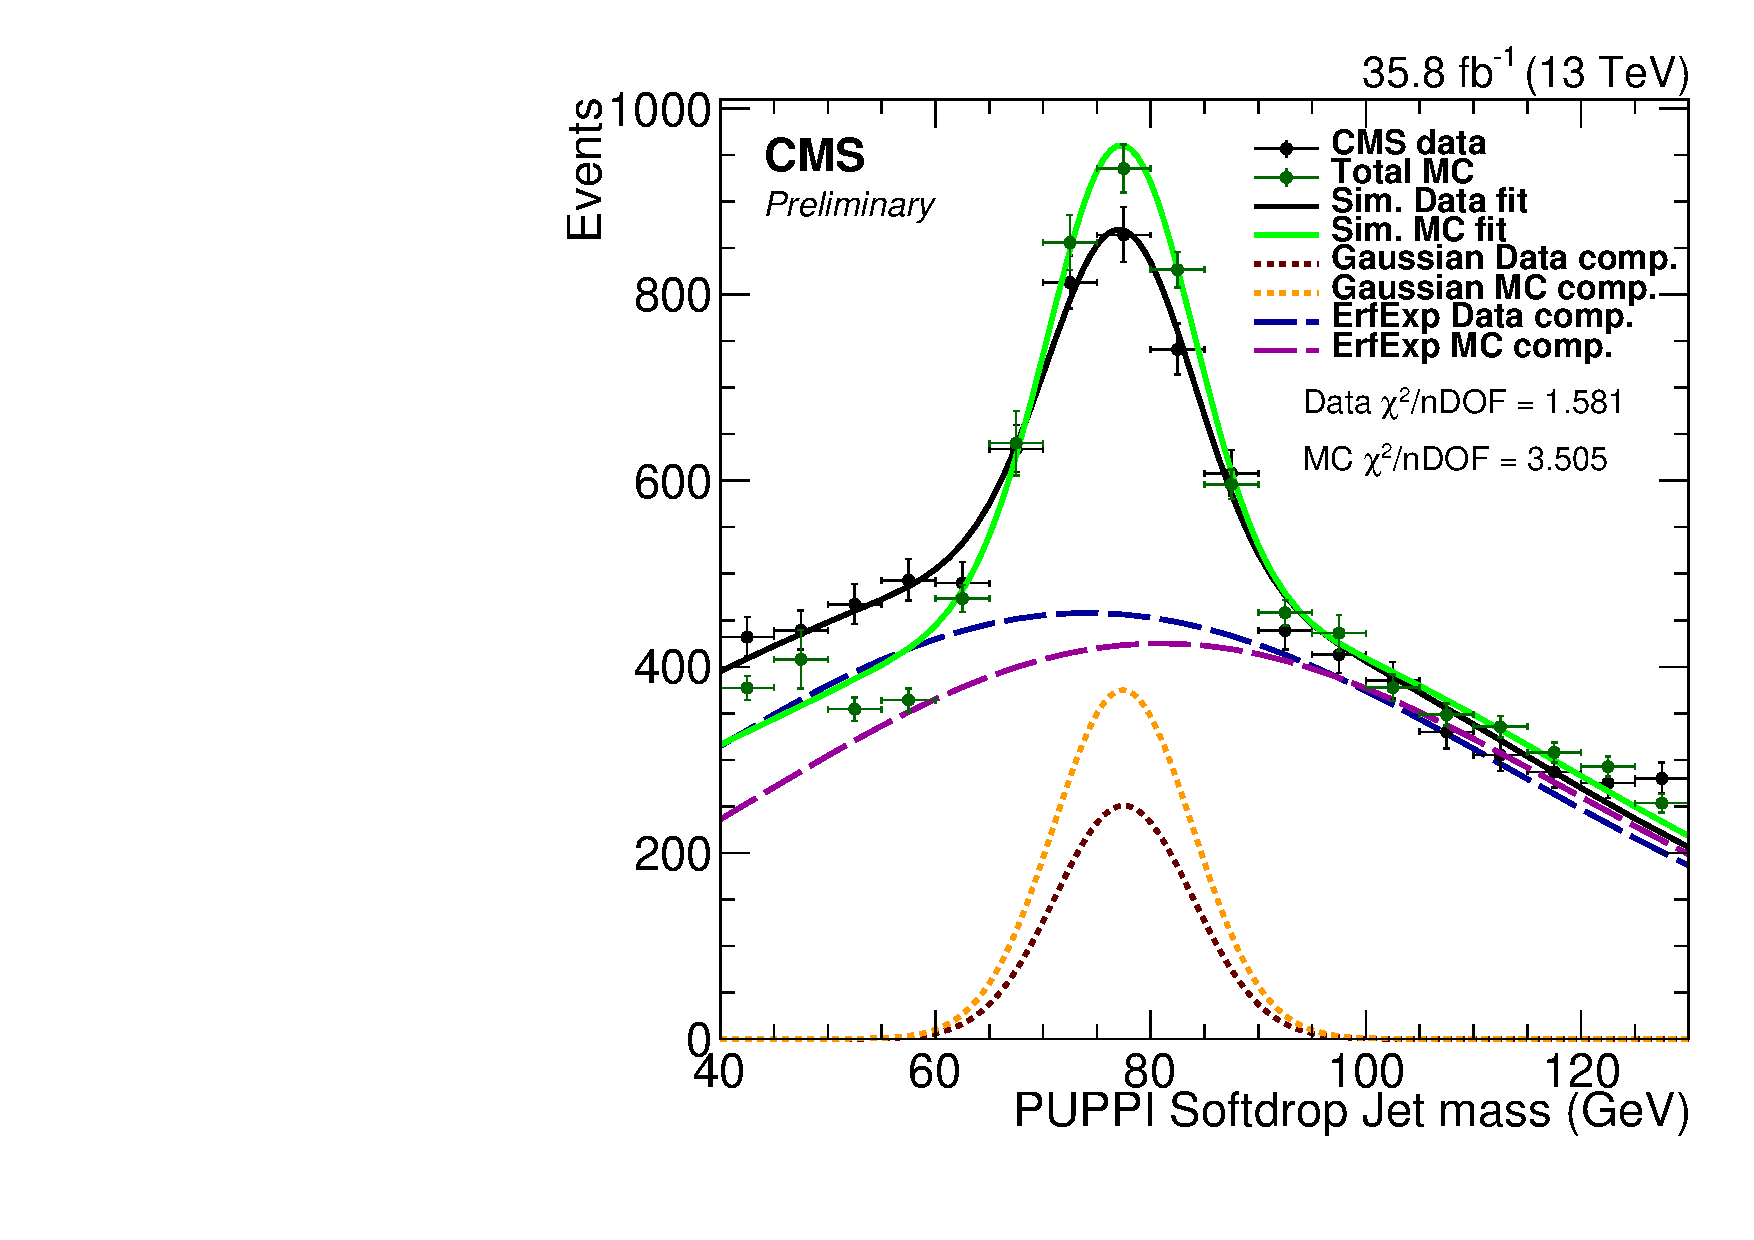
\includegraphics[width=0.45\textwidth]{figures/higgstagging/n2ddt/CombinedPlot_model_data_em_CA15.pdf}
%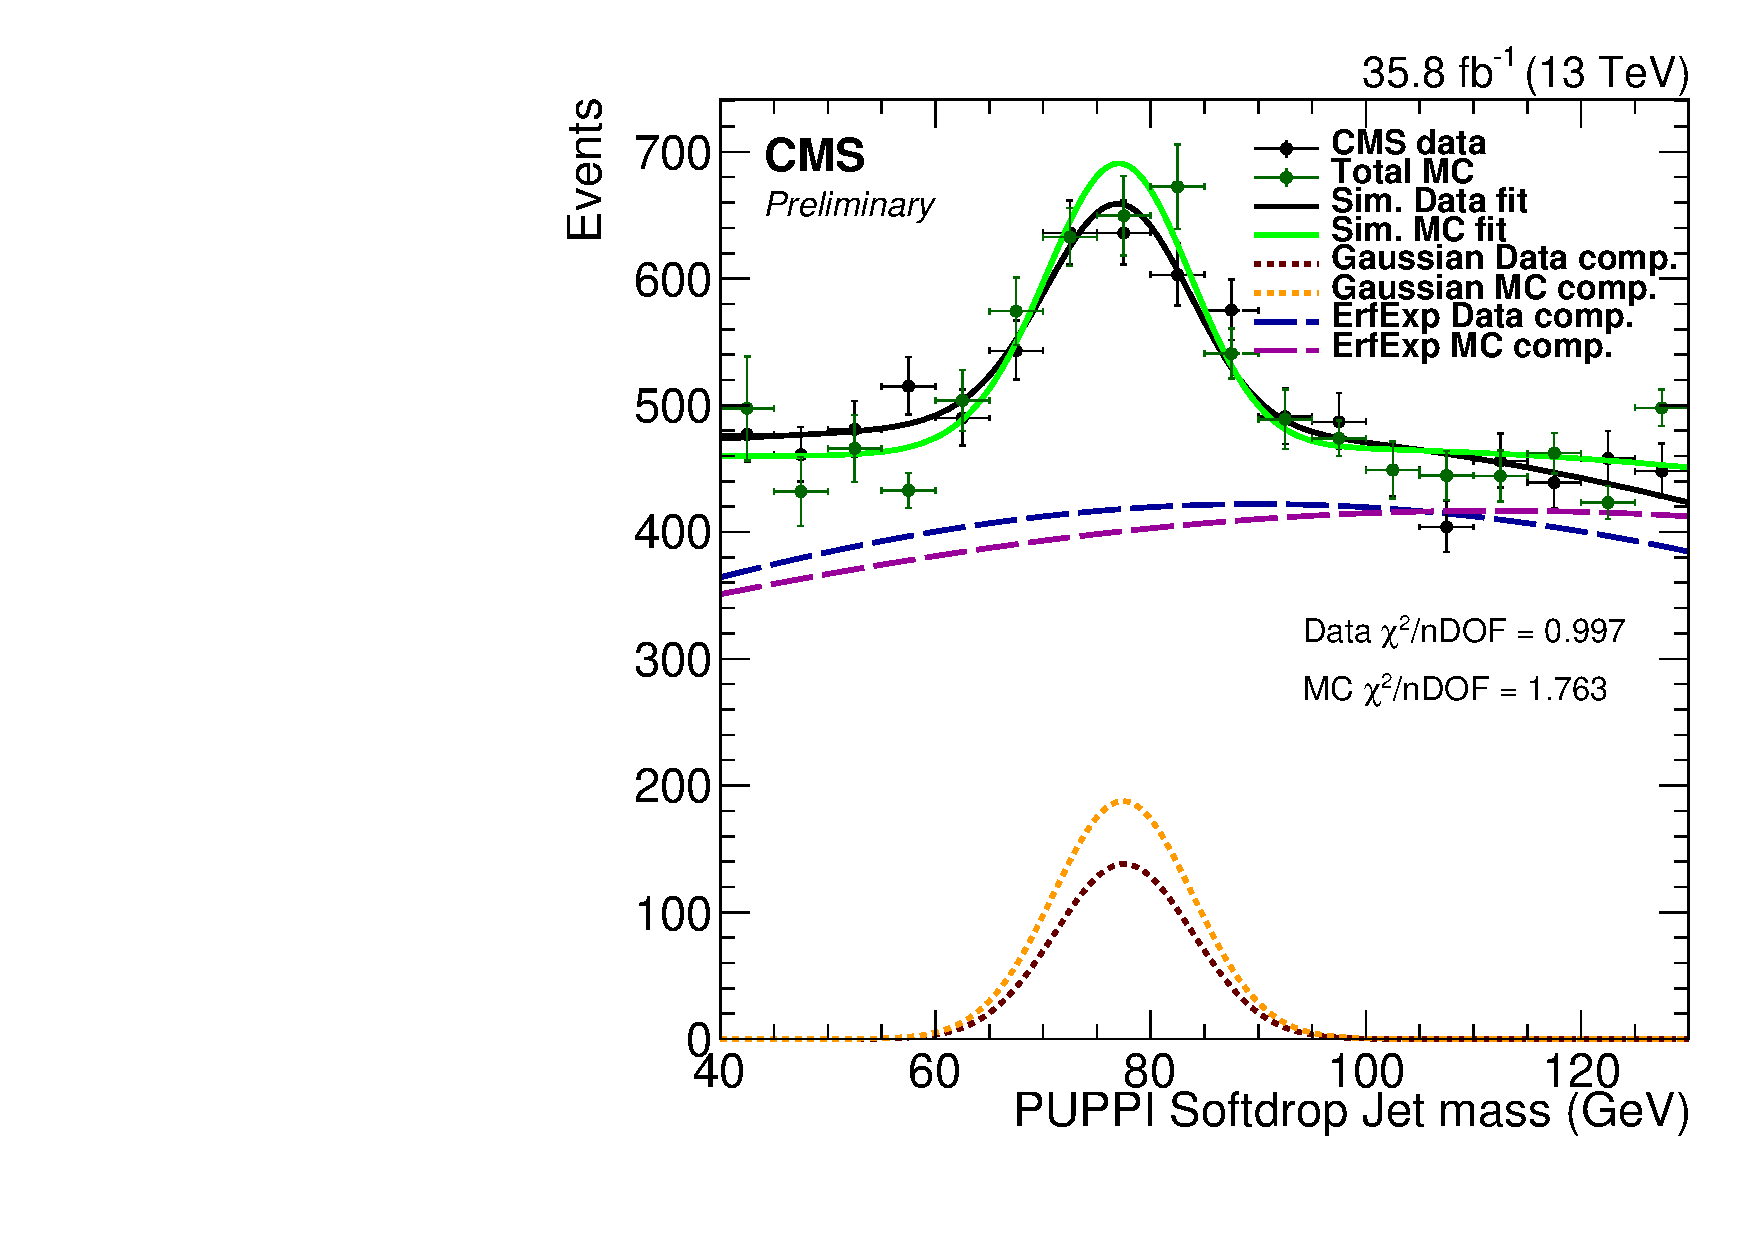
\includegraphics[width=0.45\textwidth]{figures/higgstagging/n2ddt/CombinedPlot_model_data_failN2DDTcut_em_CA15.pdf}
%\caption{Puppi softdrop mass distributions that pass(left) and fail(right) the $N_{2}^{DDT}<0$. Results are shown for both data and simulation.}
%\label{fig:TotalFits}
%\end{figure}



%Finally, Fig.~\ref{fig:n2data_1} demonstrates a very good description of the N2DDT variable in top quark jets or QCD jets dominated regions (our control regions are introduced in Section~\ref{sec:cr}). The scale factor in \ref{tab:ScaleFactors} is applied to the signal and the MC-driven backgrounds which have a massive resonances decaying into two prongs (VH, diboson). 



%\begin{figure}
%\centering
% \subfloat{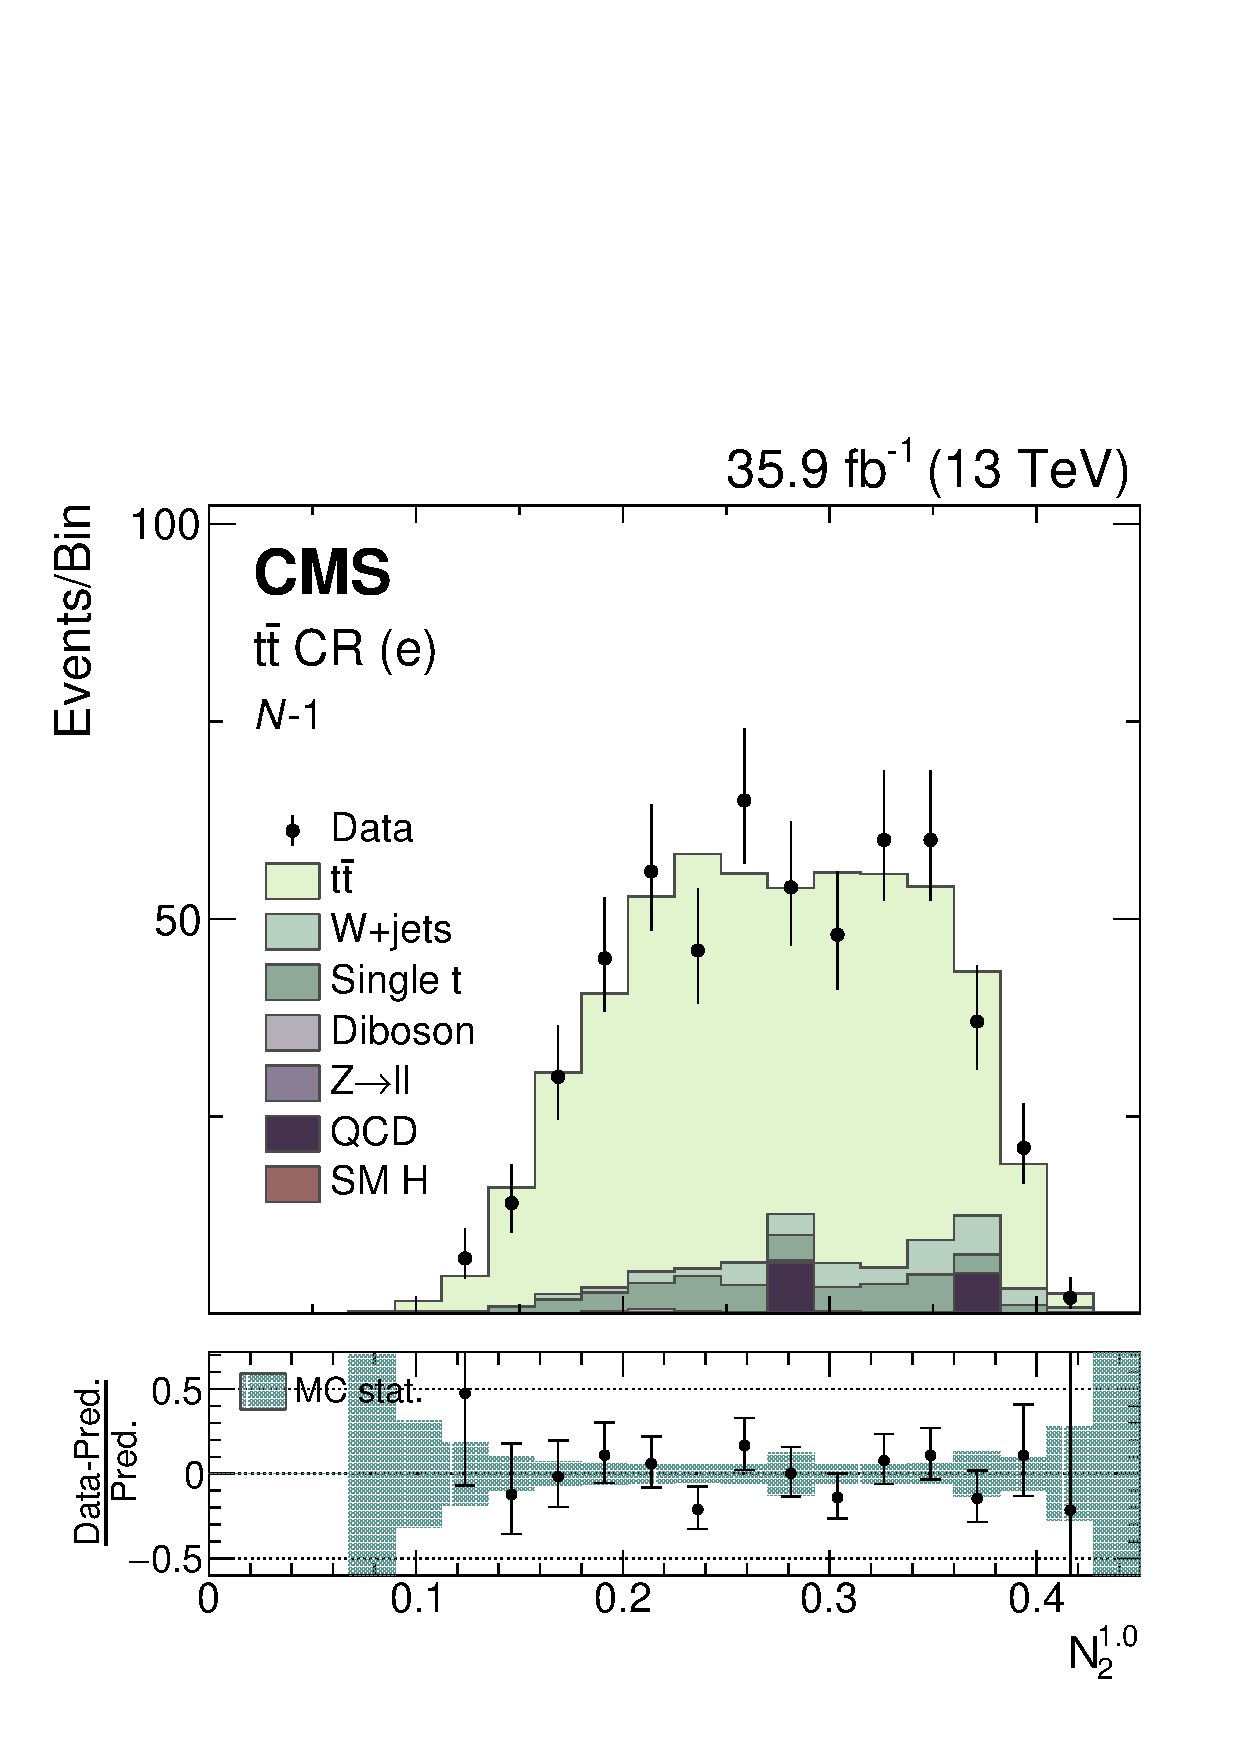
\includegraphics[width=0.33\textwidth]{figures/dataMC/cr_ttbar_el_N2_10_NM1_lumi0.pdf}}
% \subfloat{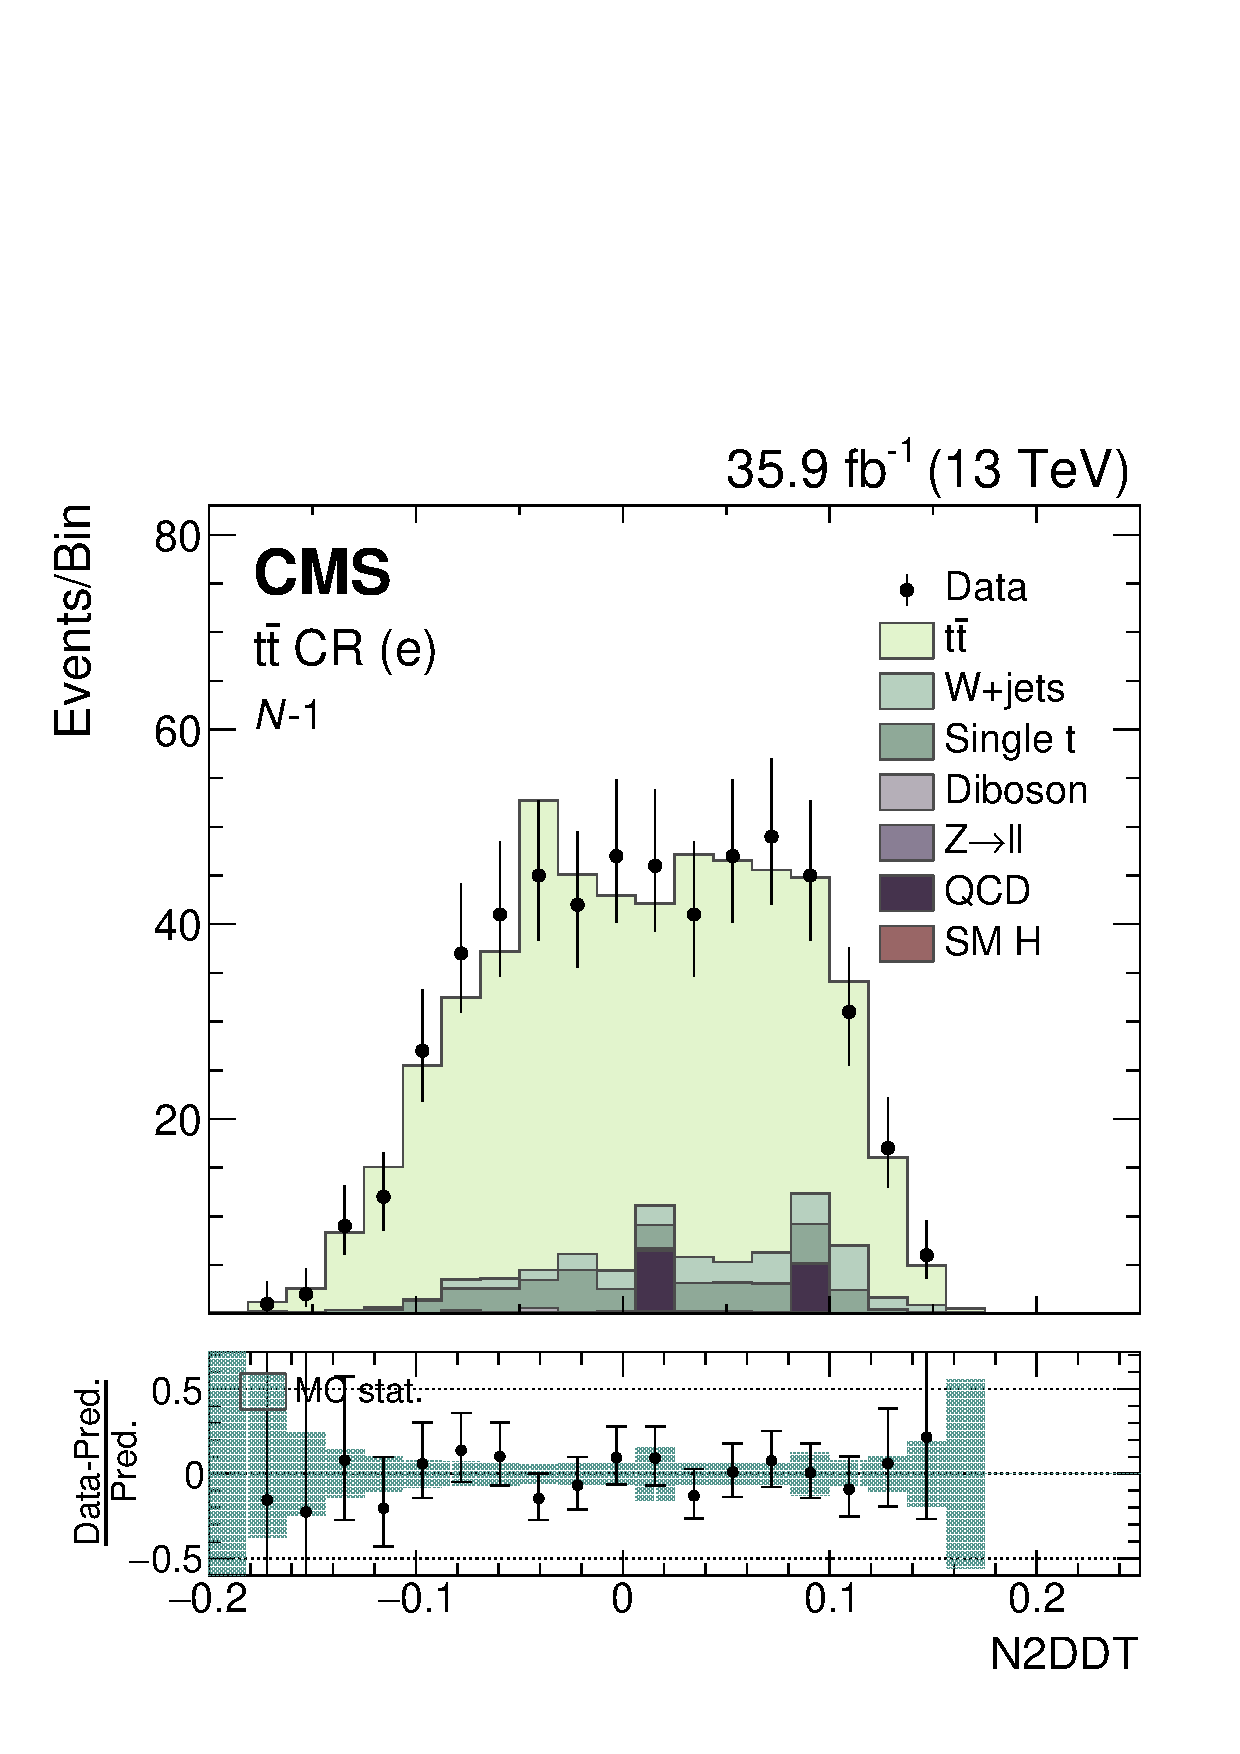
\includegraphics[width=0.33\textwidth]{figures/dataMC/cr_ttbar_el_N2DDT_NM1_lumi0.pdf}}\\
% \subfloat{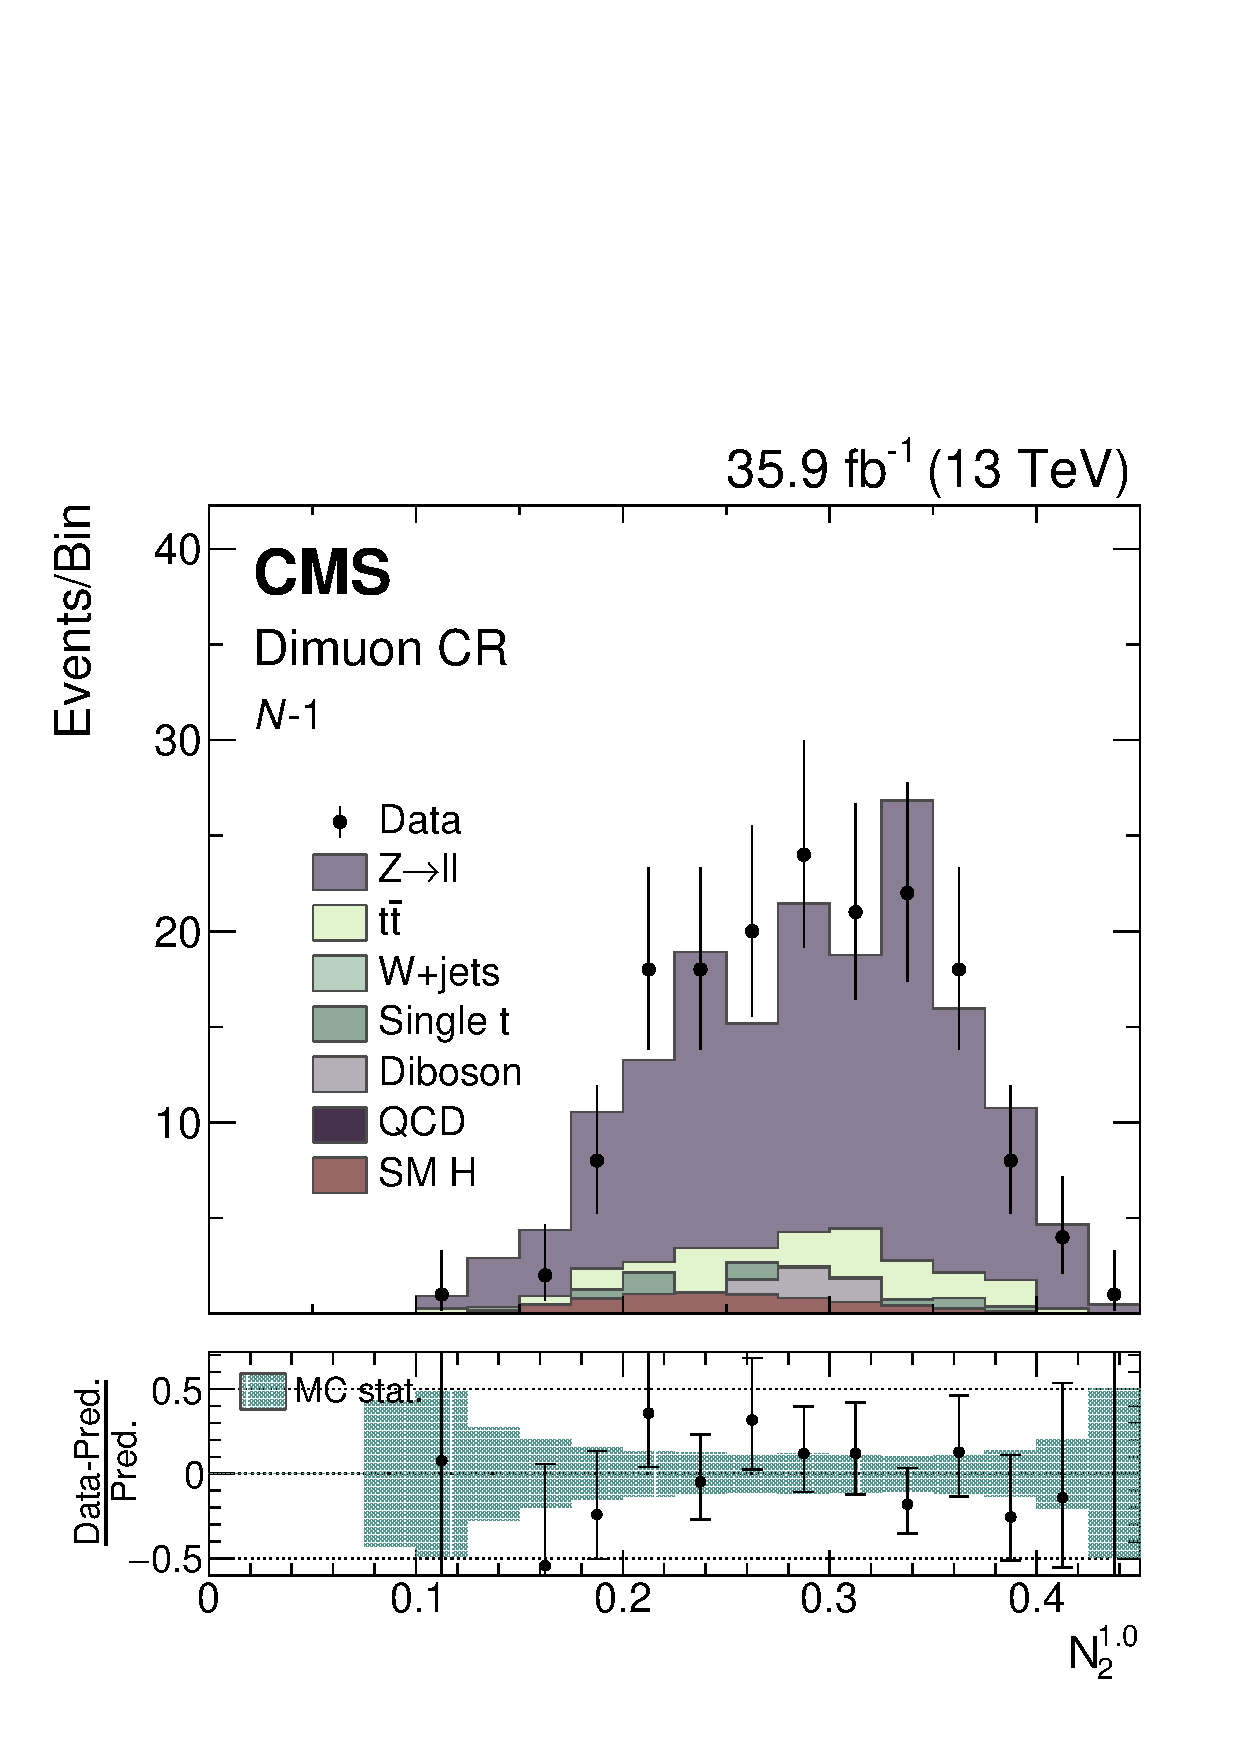
\includegraphics[width=0.33\textwidth]{figures/dataMC/cr_dimuon_N2_10_NM1_lumi0.pdf}}
% \subfloat{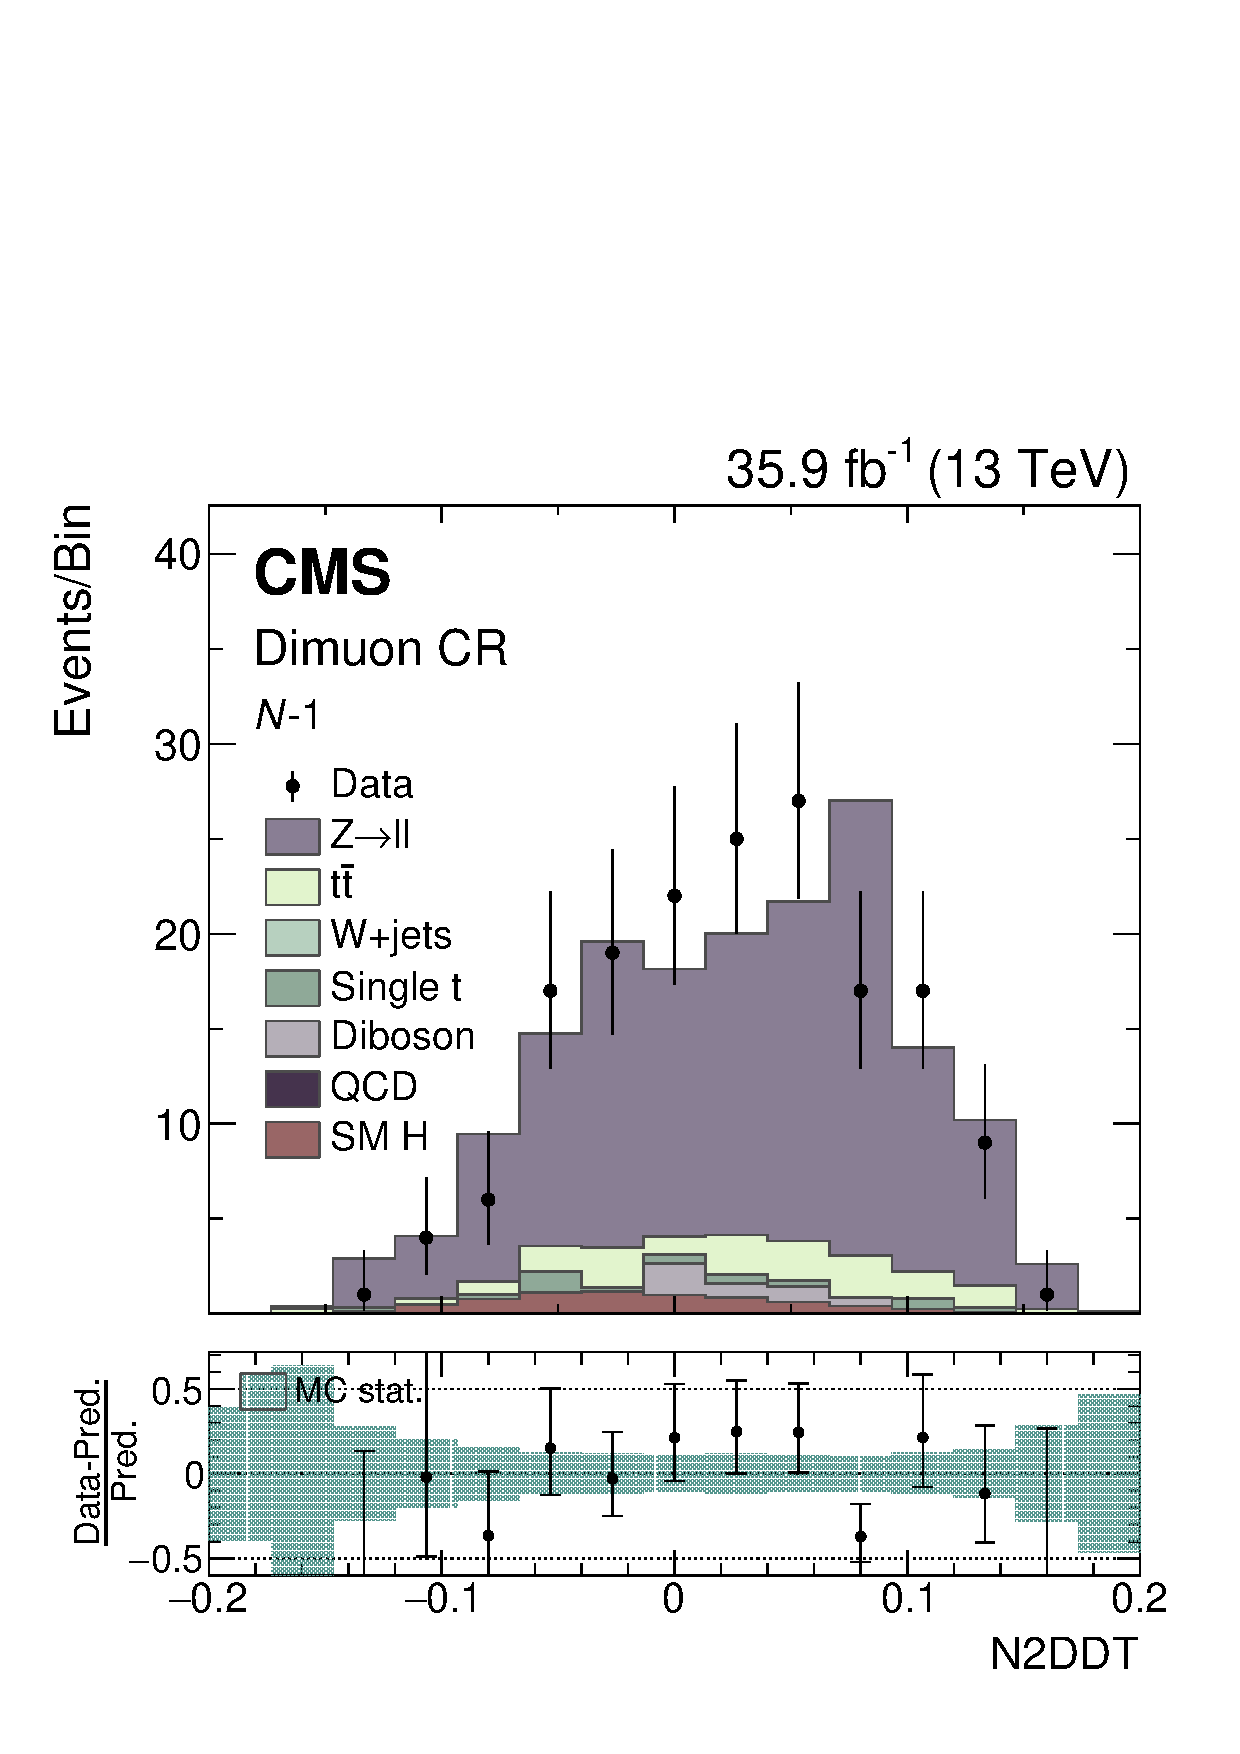
\includegraphics[width=0.33\textwidth]{figures/dataMC/cr_dimuon_N2DDT_NM1_lumi0.pdf}}\\
%\caption{Validation plots for $N_2$ and $N_2^{\text{DDT}}$  in the ttbar and dilepton control regions. No cut on N2DDT is applied. MC is normalized to data in order to facilitate the shape comparison. Very good agreement is observed. }
%\label{fig:n2data_1}
%\end{figure}




\subsection{Double-b tagger}

In this analysis we employ the double-b tagger algorithm. A general description of the tagger, which tries to identify a two-prong structure made of b quarks, is provided in~\cite{CMS-PAS-BTV-15-002}. Particularly for the CA15 case, the training of the tagger has been repeated incorporating the minimum of the CSV scores of the two leading subjets as input variables. Due to the larger cone with $R=1.5$, the clustering algorithm is able to retain a higher signal efficiency also in regimes with intermediate boost, where it is possible to clearly resolve two subjets, hence additional information can be gained from the CSV scores. This is visible from the ROC curve in Fig.~\ref{fig:doublebroc}, showing the performace of the CA15 double-b tagger version compared to tradition methods like the use of subjet CSV scores only.


\begin{figure}
  \centering
  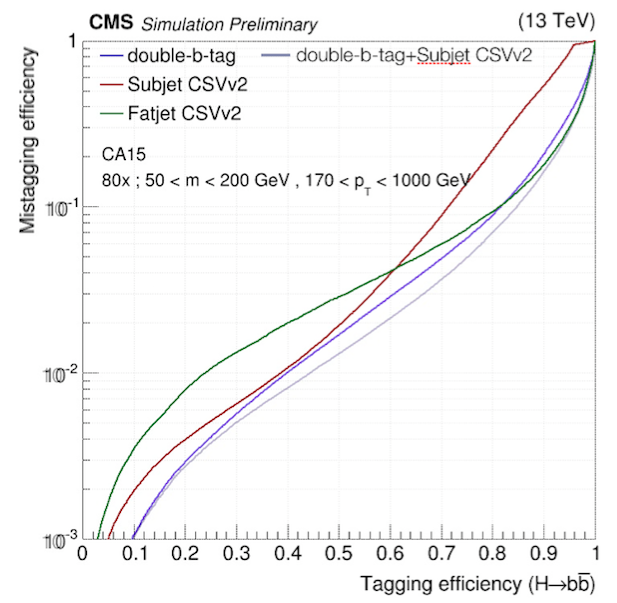
\includegraphics[width=0.475\textwidth]{figures/higgstagging/doubleb/doubleb_roc_split.png}\\
  \caption{ROC curve comparing the performance in tagging $\text{H}\to\text{b}\bar{\text{b}}$ fat jets of using either subjet CSV algorithm or double b tagger with or without the subjet CSV scores as input variables.}
  \label{fig:doublebroc}
\end{figure}

The chosen working point of double-b $> 0.75$ corresponds to the same background efficiency of the medium working point of the minimum of the CSV scores of the two leading subjets used in the previous iteration of Mono-H  analysis~\cite{monoH}, benefiting from the enhanced signal efficiency.
In terms of tagging and mistagging efficiency measurements, the analysis is precisely following what has been done in~\cite{CMS-PAS-BTV-15-002} with AK8 jets for deriving scale factors for the double-b tagger to be applied throughout the analysis. The current measurement at 13\TeV with AK8 jets is documented in~\cite{Ref:BTAG2016}. A dedicated tagging and mistagging efficiency mesurements on CA15 jet was derived~\cite{monoH} and will be applied throughout the analysis.

%\subsubsection{Tagging efficiency measurement}
%\label{tagging_efficiency}
%The Lifetime Tagging (LT) method uses the Jet Probability (JP) discriminant to measure the double-b tagging efficiency by fitting MC templates for b, c and light flavour jets to data~\cite{Ref:LT}. This discriminant uses information on the probability of tracks in a jet with positive impact parameter significance to originate from the primary interaction vertex. This parameter is calibrated in inclusive QCD multijet events using templates with negative impact parameter tracks~\cite{Ref:JP}. The calibration is performed independently in data and MC. The JP discriminant provides a good shape separation between heavy and light flavour jets over the broad jet \pt range and can be used as a fit variable to extract the fraction of heavy flavour jets in data sample.

%In the absence of a control region clean enough in Hbb events, the measurement is performed in double-muon tagged multijet events, which are enriched in gbb events serving as a good proxy for Hbb decays, as was reasoned in~\cite{CMS-PAS-BTV-15-002}. The simulated datasets used are listed in Tab.~\ref{Tab:QCDMultijet}. Muon−enriched samples obtained by requiring a muon with $\pt> 5\GeV$ at the generator level are used in association with BTagMu data corresponding to the full integrated luminosity available from the year 2016. Triggers as listed in Tab.~\ref{Tab:Triggers} are employed.




%\begin{table}[htb]
% \begin{center}
%\footnotesize
%  \caption{QCD MC samples used in the efficiency measurement.}
%\begin{tabular}{lr}
%\hline\hline
%{\bf Muon-enriched MC} & \\
%\vspace{2mm} Sample & $\sigma $ [pb]  \\
%\hline
%QCD\_Pt\_170to300\_MuEnrichedPt5\_TuneCUETP8M1\_13TeV\_pythia8 & $8.65 \cdot 10^3$ \\
%QCD\_Pt\_300to470\_MuEnrichedPt5\_TuneCUETP8M1\_13TeV\_pythia8 & $7.97 \cdot 10^2$ \\
%QCD\_Pt\_470to600\_MuEnrichedPt5\_TuneCUETP8M1\_13TeV\_pythia8 & $7.90 \cdot 10^1$ \\
%QCD\_Pt\_600to800\_MuEnrichedPt5\_TuneCUETP8M1\_13TeV\_pythia8 & $2.51 \cdot 10^1$ \\
%QCD\_Pt\_800to1000\_MuEnrichedPt5\_TuneCUETP8M1\_13TeV\_pythia8 & $4.71$ \\
%QCD\_Pt\_1000toInf\_MuEnrichedPt5\_TuneCUETP8M1\_13TeV\_pythia8 & $1.62$ \\
%\hline
%\end{tabular}
%\normalsize
%  \label{Tab:QCDMultijet}
%\end{center}
%\end{table}

%CA15 jets with $|\eta| < 2.4$ were selected, with the jets passing the ``tight'' jet ID requirement~\cite{JetID13TeVTWiki}. The soft drop algorithm was used to resolve the CA15 jets into substructures, henceforth called soft drop subjets. Muon-tagging of jets is used to enrich them in $B$ hadrons. Both the subjet and the double-b tagger performance measurements use AK8 jets containing muon-tagged subjets, with the following muon ID requirement:

%\begin{itemize}
%\item Global PF muon with $\pt > 7\GeV$ and $|\eta| < 2.4$;
%\item N (hits in muon chambers) $> 0$;
%\item N(matched muon stations) $> 1$;
%\item N(hits in tracker layers) $> 7$;
%\item N(hits in pixel layers) $> 0$;
%\item N(missing outer hits) $< 99$;
%\item $\chi^{2}$/ndf from global track $< 10$;
%\item $\pt(\mu)/\pt({\rm jet})  < 0.5$;
%\item $\Delta R(\mu, {\rm subjet}) < 0.4$;
%\end{itemize}

%For the double b-tagger measurements, the CA15 jets are required to have $\pt > 200\GeV$, divided in the ``low \pt'' ($200 < \pt < 350\GeV$) and the ``high \pt'' ($\pt > 350\GeV$) ranges. We use the official pile-up reweighting, as well as MC JP calibration on both data and MC.
%We reweight the MC $\pt$ distribution to match the data distribution in order to account for triggers being absent from certain data runs. Lastly, we remove any jet from a QCD sample with $p_{T}$ $<$ 300 GeV that has high weight or that comes from an event with high jet multiplicity, in order to prevent large spikes in the JP distribution used to calculate the scale factor.

%The final selection features:

%\begin{itemize}
%\item Muon $p_\text{T}\text{'s}>7$\,GeV
%\item $\text{pruned~jet~mass}>50$\,GeV
%\item $p_\text{T}(\mu_1+\mu_2)<0.6\,p_\text{T}(\text{jet})$ in order to guarantee for sufficient hadronic activity in the jet 
%\end{itemize}


%\begin{table}[htbp]
%  \begin{center}
%    \topcaption{Trigger requirements for double b-tagging in different \pt bins.}\label{tab:BoostedTrigs}
%    \begin{tabular}{c|c} 
%      \hline\hline
%      Range in fat jet \pt & Trigger\\ 
%      \hline 
%      $>350$ &    \texttt{BTagMu\_AK8Jet300\_Mu5} \\
%      200-350 & \texttt{BTagMu\_DiJet170\_Mu5} \\
%      \hline\hline
%    \end{tabular}
%  \label{Tab:Triggers}
%  \end{center}
%\end{table}


%Commissioning plots of some of the input variables are presented in Fig.~\ref{fig:doublebdata_1}. The final double-b tagger discriminant is shown in the same Figure, as is the JP distribution that is used for extracting the scale factor in the fit explained in the following. Shapes for the different components for both \pt bins are shown in Fig.~\ref{fig:double_shapes} for the pretag and pass regions. The properly normalized postfit templates are shown in \ref{fig:double_shapes_norm}.

%\begin{figure}
%\centering
% \subfloat{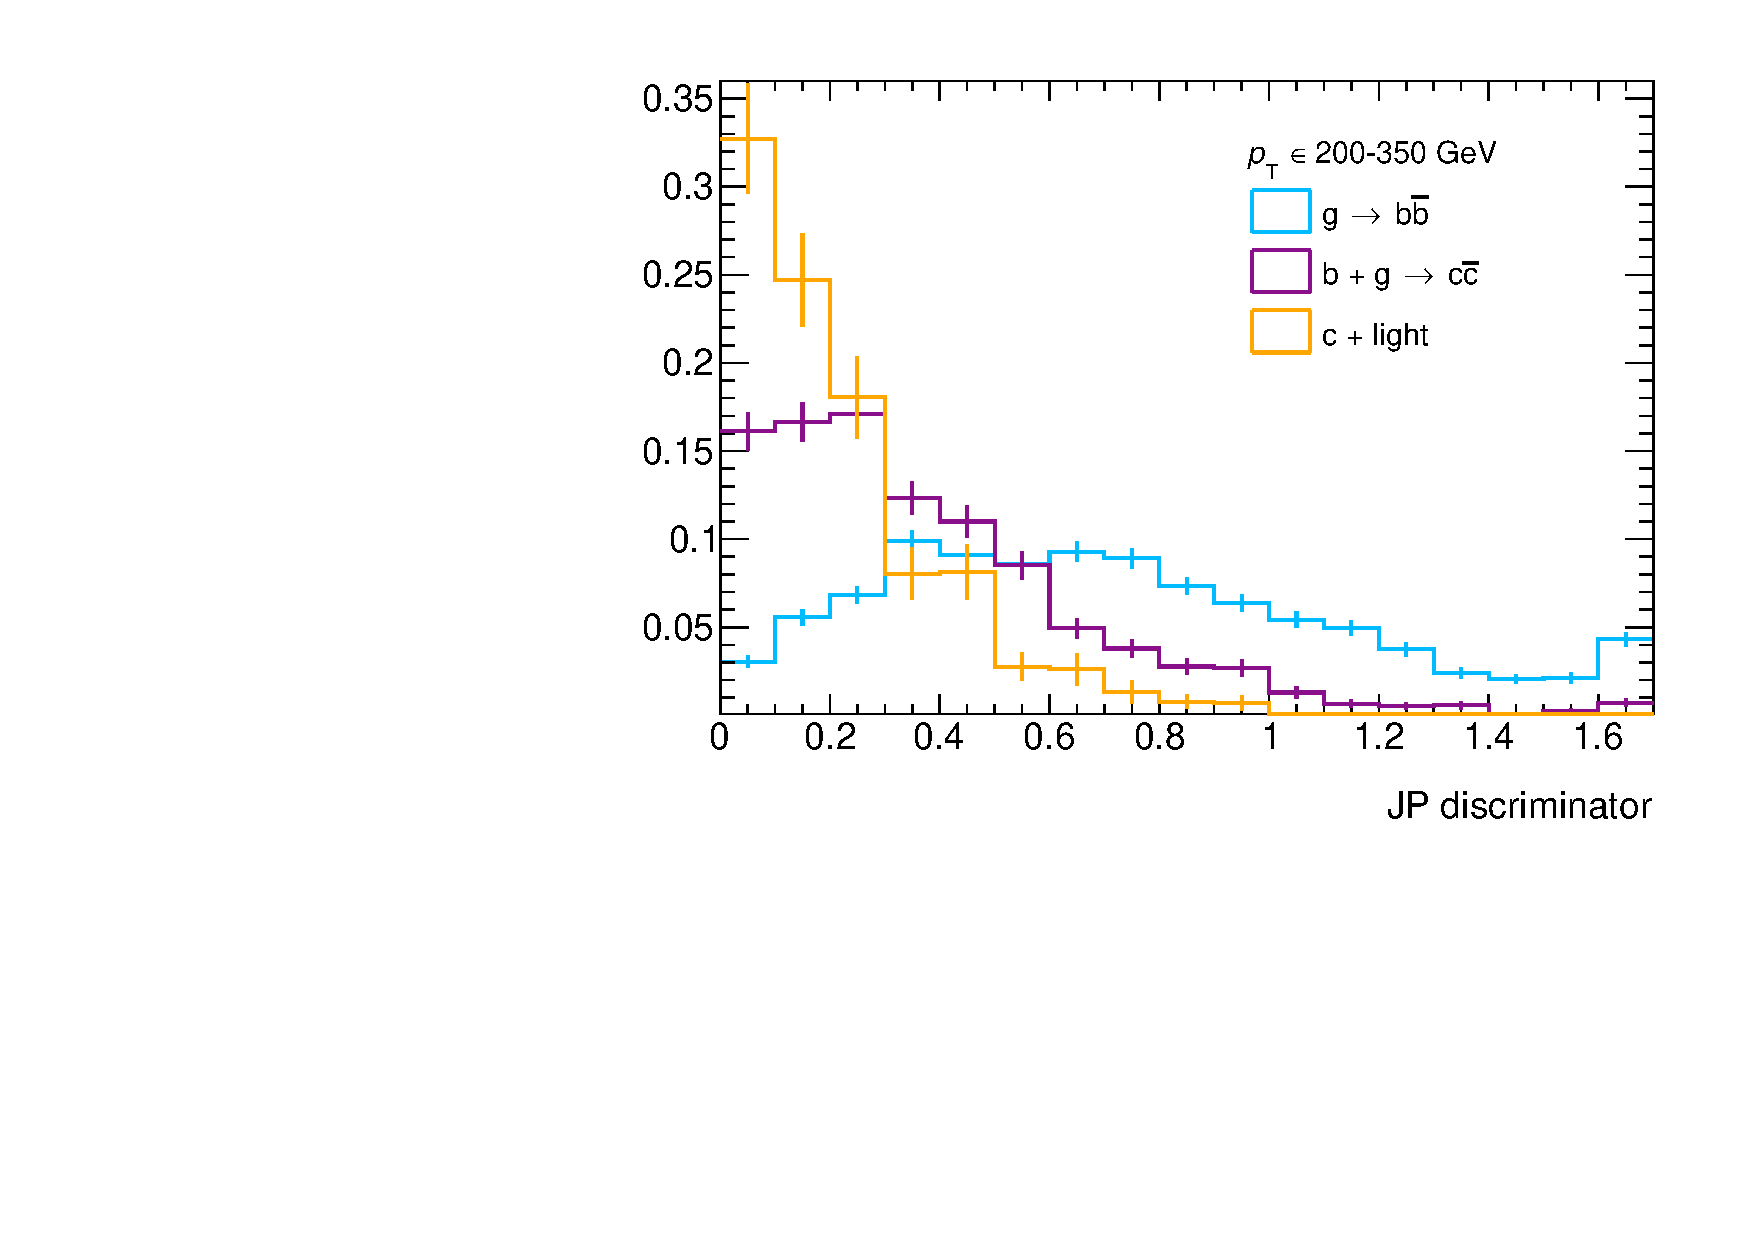
\includegraphics[width=0.45\textwidth]{figures/higgstagging/doubleb/doubleBM2ptlow/pics/shape.pdf}}
% \subfloat{\includegraphics[width=0.45\textwidth]{figures/higgstagging/doubleb/doubleBM2pthigh/pics/shape.pdf}}\\
% \subfloat{\includegraphics[width=0.45\textwidth]{figures/higgstagging/doubleb/doubleBM2ptlow/pics/shape_tag.pdf}}
% \subfloat{\includegraphics[width=0.45\textwidth]{figures/higgstagging/doubleb/doubleBM2pthigh/pics/shape_tag.pdf}}\\
%\caption{Shape comparison of the jet probability in the double-muon tagged multijet samples for various flavours contained in the fat jet for the pretag region (top row) and the pass bin (bottom row), for both \pt bins.}
%\label{fig:double_shapes}
%\end{figure}

%\begin{figure}
%\centering
% \subfloat{\includegraphics[width=0.45\textwidth]{figures/higgstagging/doubleb/doubleBM2ptlow/pics/shape_norm.pdf}}
% \subfloat{\includegraphics[width=0.45\textwidth]{figures/higgstagging/doubleb/doubleBM2pthigh/pics/shape_norm.pdf}}\\
% \subfloat{\includegraphics[width=0.45\textwidth]{figures/higgstagging/doubleb/doubleBM2ptlow/pics/shape_tag_norm.pdf}}
% \subfloat{\includegraphics[width=0.45\textwidth]{figures/higgstagging/doubleb/doubleBM2pthigh/pics/shape_tag_norm.pdf}}\\
%\caption{Comparison of the jet probability in the double-muon tagged multijet samples for various flavours contained in the fat jet for the pretag region (top row) and the pass bin (bottom row), for both \pt bins, normalized to the postfit yields. For the signal template, also the prefit distribution is shown. The SF of 0.91 for the low-$p_\text{T}$~bin is reflected in the difference between the blue and red templates comparing prefit and postfit, respectively.}
%\label{fig:double_shapes_norm}
%\end{figure}


%Given the discimination power of this variable, by fitting separately in both the pretag and pass regions, the relative fractions of the various flavours can be determined, and a scale factor given by 

%\begin{equation}
%\text{SF}=\frac{\epsilon_{\text{data}}}{\epsilon_{g\to b\bar{b}~\text{MC}}},
%\end{equation}

%where data is understood to be represented by the $g\to b\bar{b}$ postfit templates.
%As several background processes are being varied as a combined template in the fit procedure, the results are sensitive to the prediction of the flavour composition of this background sample. Before applying the b tagging requirement, two background templates are considered. Contributions from single-b production and c from gluon splitting are combined together, as well as single-c and light jets. After the tagging all background processes are treated as one template. The fitted distributions for JP discriminant in the pretag region as well as in the pass bin are presented in Fig.~\ref{fig:doublebdata_2}. 

%A corresponding uncertainty on the scale factor is estimated by conservatively varying the normalization of each subcontribution of background by $\pm 50\%$. As a cross check, the scale factor derivation is also performed using all subcontributions as individual templates in the fit. Systematics related to the JP calibration are calculated by comparing the scale factor calculated using MC JP calibration on data and MC (nominal) to the scale factor calculated using data JP calibration on data and MC calibration on MC. Several sources of systematic uncertainties are accounted for. The systematics on the scale factor due to jet energy corrections, bad modelling of the number of tracks distributions, the branching ratios for c hadrons to muons, the b and fragmentation function, uncertainties on the fragmentation rate of a c quark to various D mesons, and the K$_S$ and $\Lambda$ fraction, are all found to be negiligble. The dominant systematic uncertainties are coming from varying the single-b or c from gluon content down/up by 50\% and by applying the data JP calibration (instead of the MC JP calibration) to data. These uncertainties amount to $\sim2\%$ on the scale factor. The final scale factor are provided in Table~\ref{tab:Doubleb_FitParameters1}. These scale factors are used in the maximum-likelihood fit explained in Section~\ref{sec:results} to correct the signal process and VH processes. Contributions from events with a $g\to b\bar{b}$-induced fat jet will be corrected in-situ during the fit with appropriate scale factors that apply to the soup of QCD jets accompanying W or Z bosons (i.e. in the W+jets or Z+jets background). More details are provided there.





%\begin{figure}
%\centering
% \subfloat{\includegraphics[width=0.475\textwidth]{figures/higgstagging/doubleb/FatJet_z_ratio_Log}}
% \subfloat{\includegraphics[width=0.475\textwidth]{figures/higgstagging/doubleb/FatJet_tau1_trackSip3dSig_0_Log}}\\
% \subfloat{\includegraphics[width=0.475\textwidth]{figures/higgstagging/doubleb/FatJet_jetNTracks_Log}}
% \subfloat{\includegraphics[width=0.475\textwidth]{figures/higgstagging/doubleb/FatJet_tau2_vertexMass_Log}}\\
% \subfloat{\includegraphics[width=0.475\textwidth]{figures/higgstagging/doubleb/FatJet_nSV_Log}}
% \subfloat{\includegraphics[width=0.475\textwidth]{figures/higgstagging/doubleb/FatJet_tau1_vertexDeltaR_Log}}\\
% \subfloat{\includegraphics[width=0.475\textwidth]{figures/higgstagging/doubleb/FatJet_DoubleB_Log}}
% \subfloat{\includegraphics[width=0.475\textwidth]{figures/higgstagging/doubleb/FatJet_JP_Log}}\\
%\caption{Validation plots of some of the input variables in the double-muon tagged multijet samples. The bottom row shows the resulting double-b tagger distribution and the JP.}
%\label{fig:doublebdata_1}
%\end{figure}

%\begin{figure}
%\centering
% \subfloat{\includegraphics[width=0.45\textwidth]{figures/higgstagging/doubleb/doubleBM2ptlow/pics/result.pdf}}
% \subfloat{\includegraphics[width=0.45\textwidth]{figures/higgstagging/doubleb/doubleBM2pthigh/pics/result.pdf}}\\
% \subfloat{\includegraphics[width=0.45\textwidth]{figures/higgstagging/doubleb/doubleBM2ptlow/pics/result_tag.pdf}}
% \subfloat{\includegraphics[width=0.45\textwidth]{figures/higgstagging/doubleb/doubleBM2pthigh/pics/result_tag.pdf}}\\
%\caption{Top row: pre-double-b-tag postfit JP distributions. Bottom row: postfit JP distributions of the events passing the double-b cut. Very good postfit agreement is observed for both the low ($<350\GeV$) and high ($>350\GeV$) \pt region.}
%\label{fig:doublebdata_2}
%\end{figure}



%\begin{table}[htbH]\footnotesize
%  \begin{center}
%  \topcaption{Fit results for the efficiency scale factor measurement corresponding to a double-b cut $>0.75$.}
%  \label{tab:Doubleb_FitParameters1}
%  \begin{tabular}{  l | c  | c | c  | c | c | c | c }
%  \hline
%  \hline
%     $p_\text{T}$ (GeV) & $\chi^2/\text{NDoF}$ & $\epsilon$ (MC) & $\epsilon$ (data) & \textbf{SF} &stat & sys up & sys down\\ \midrule
%     \hline
%200-350 & 1.04& $0.71\pm0.01$ & $0.65\pm0.04$ &  $\textbf{0.91}\pm\textbf{0.03}$ &  0.029 & 0.011 & 0.019\\ \hline

%$>350$ & 1.91 & $0.61\pm0.01$ & $0.61\pm0.03$ & $\textbf{1.00}\pm\textbf{0.04}$ & 0.024 & 0.013 & 0.032\\ \hline
%     \hline
%     \hline
%  \end{tabular}
%  \end{center}
%\end{table}


%\subsubsection{Mistagging efficiency measurement for top quark jets}
%\label{mistag_efficiency}

%One dominant source of background is semi-leptonic \ttbar production where the lepton is lost either because it is out of acceptance or does not pass the criteria imposed in the selection. In the mass window between 100\GeV and 150\GeV, the absolute fake rate of top quark induced fat jets for the chosen double-b working point is about 14\%. With the top quark being resonantly produced in the vicinity of the our signal region mass window (as opposed to the combinatorial background arising from QCD radiation inducing fat jets such as, for example, in Z+jets), we perform a dedicated mistag measurement for the top quark induced fat jets, following the strategy of~\cite{CMS-PAS-BTV-15-002}. We define a \ttbar enriched region orthogonal to our nominal top control region introduced in Section~\ref{sec:cr} by inverting the requirement on the number of allowed additional AK4 jets and by widening the window on the fat jet soft drop mass to 50-250\GeV. This ensures a flavor composition in the fat jets that is similar to the one found in our signal region, which is mostly comprised of fat jets that contain the b quark and one light quark of the top quark (and subsequent W boson) decay.


%\begin{figure}[h]
%\centering
%\includegraphics[width=0.45\textwidth]{figures/dataMC/cr_ttbar_mu_fj1DoubleCSV_2prong.pdf}
%\includegraphics[width=0.45\textwidth]{figures/higgstagging/cr_ttbar_mu_fj1DoubleCSV.pdf}\\
%\includegraphics[width=0.4\textwidth]{figures/dataMC/cr_ttbar_mu_fj1DoubleCSV_sf.pdf}\\
%\caption{Top row: data vs. MC comparison in the combined e+$\mu$ \ttbar~CR with inverted requirement on the number of isolated AK4 jets (left). The ``Top'' templates contain contributions from both \ttbar and single top processes.  They are split up into different quark content of the fat jet. Just as for the signal region, the main contribution comes from events with ``unmatched'' top quarks where the fat jet contains a b and a light quark. Background-subtracted data (i.e. data minus W+jets, single top, diboson predictions) is compared to only the \ttbar simulation (this time not split up) in the upper right figure, from which the scale factor is computed. The red arrow indicates the double-b working point. Bottom row: the scale factor is given by the ratio of efficiencies of double-b score $>0.75$ in data and MC.}
%\label{fig:ttbarmistag}
%\end{figure}

%Then, all non-\ttbar background is subtracted from data, and the mistag SF is given by the ratio of efficiencies found in background-subtracted data and \ttbar simulation, as shown in Figure~\ref{fig:ttbarmistag}. A 30\% uncertainty on the subtracted backgrounds (mostly single top and W+jets) is applied, resulting in a scale factor of $1.03\pm0.03(\text{stat.})\pm0.07(\text{syst.})$. The \ttbar~reweighting has been applied in this measurement. Not applying this correction results in a 1\% effect on the scale factor; we therefore neglect this source of systematic uncertainty. 

%The scale factor will serve as prior for the parameter that extracts the relative normalization of \ttbar between bins passing or failing the double-b cut in-situ from the maximum-likelihood fit described in Section~\ref{sec:results}.

%A measurement binned in fat jet \pt gives consistent results and is found to have no impact on the final sensitivity of the analysis. All \ttbar mistag scale factors are listed in Table~\ref{tab:Doubleb_FitParameters2}.


%\begin{table}[htbH]
%  \begin{center}
%  \topcaption{Mistag scale factor measurement for top quark jets.}
%  \label{tab:Doubleb_FitParameters2}
%  \begin{tabular}{  l | c  | c | c  }
%  \hline
%  \hline
%     $p_\text{T}$ (GeV) & \textbf{SF} &stat & sys \\ \midrule
%     \hline
%inclusive & $\textbf{1.03}$ & 0.03 & 0.07\\ \hline
%200-350 & $\textbf{1.04}$ & 0.04 & 0.07\\ \hline
%350-500 & $\textbf{1.00}$ & 0.07 & 0.08\\ \hline
%$>500$ & $\textbf{1.02}$ & 0.17 & 0.21\\ 
%     \hline
%     \hline
%  \end{tabular}
%  \end{center}
%\end{table}


 %edit soft drop plot base on PUPPI

\cleardoublepage
\section{Event selection}
\label{sec:cr}


The preselection common to all regions (signal and control regions) is:

\begin{itemize}
\item exactly one CA15 fat jet with $\textit{p}_\text{T}>\text{200}$\,GeV and $|\eta|<\text{2.4}$ 
\item fat jet soft drop mass between 100 and 150\GeV
\item PF $\text{MET}>\text{250}$\,GeV (SR) or PF recoil $>\text{250}$\,GeV (CR) 
\item $\Delta \phi(\text{AK4~jets,MET/Recoil})>\text{0.4}$
\item $\tau$ and photon veto
\item not more than one additional AK4 jet
\item $N_2^\text{DDT}<0$
\end{itemize}

This already ensures a topology very close to the one expected by the monoH signal. Then lepton multiplicities and the number of b tagged AK4 jets which are not overlapping with the fat jet are used to distinguish between the signal and control regions in order to keep the extrapolation uncertainties at a minimum.

\begin{table}
  \begin{center}
  \caption{Event selection table. Common to all regions is a preselection} \label{tab:event_selection}
    \begin{tabular}{  l | c | c | c  }
      \hline \hline
        region   & iso AK4 b tags   & leptons & double-b  \\ \hline
        signal   & 0                & 0       & pass \\ \hline
        \ttbar   & 1                & 1       & pass/fail\\ \hline
        W        & 0                & 1       & pass/fail\\ \hline
        Dilepton & 0                & 2       & pass/fail\\
      \hline \hline
    \end{tabular}
  \end{center}
\end{table}


Finally, the control regions are split up into pass/fail regions depending on whether or not they pass the cut on the double-b tagger of $>0.75$ so that in total, we end up with 12 control regions ($[\text{t}\bar{\text{t}},\text{W},\text{Dilepton}]\times[e,\mu]\times[\text{pass,fail}]$). With respect to the other mono-X analyses, this analysis is not making use of a photon control region. The impact of having or removing such control region has been estimated to be of the order of a few \% on the overall mono-Higgs sensitivity. This is mainly due to the fact that the higher contribution of $t\bar{t}$ production to the overall background makes the impact of a tighter constrain on the $Z$+jets background, like the one given by the events with photons, less important for this search. Furthermore the simultaneous use of dilepton pass and fail control region enhances the statistical power, limiting the necessity of adding a high statistics control sample like the one composed by events with photons. Table~\ref{tab:event_selection} summarizes the selection. Key distributions for all the control regions are presented in Fig.~\ref{Fig_cr_ttbar_mu_1}-\ref{Fig_cr_dielectron_1}. In all distributions, MC is normalized to prediction. Recoil distributions are shown in Fig.~\ref{Fig_cr_Recoil}-\ref{Fig_cr_Recoil_fail}. In general, a very good shape agreement is observed. In the final fit, a scale factor is allowed to float that adjusts the relative normalization of the dominating backgrounds in the pass/fail categories. More details are given in Section~\ref{sec:results}. Finer binned versions of the recoil variables are presented in Fig.~\ref{Fig_cr_Recoil_fine}-\ref{Fig_cr_Recoil_fail_fine}.

Finally, the unblinded \ptmiss~distribution in the signal region is shown in Fig.~\ref{Fig_sr}. Fig.\ref{Fig_sr_content} in the Appendix gives more details as far as the quark content inside the fat jet for the main backgrounds is concerned. A slight excess is observed in events with higher \ptmiss. As the limits will show, this is compatible with SM background predictions within the 1$\sigma$ level once including all systematic uncertainties.

\clearpage

\begin{table}\footnotesize
\begin{center}
  \caption{Prefit event yield expectations for the \ttbar control regions. Uncertainties are statistical only.} \label{tab:yield_ttbar}
\begin{tabular}{l r  r r r}
  \hline\hline
Process       & \ttbar $\mu$   & \ttbar e     & \ttbar fail $\mu$  & \ttbar fail e\\ 
\hline
QCD           &$ 0.6 \pm 0.6  $&$ 0\pm0$      & $ 27.8 \pm 20.9  $ &$ 34.3\pm20.6$\\
DY            &$ 0.8 \pm 0.3 $ &$ 0.4\pm0.2$  & $ 20.4 \pm 1.9 $   &$ 6.5\pm1.0$\\
Diboson       &$ 1.1\pm0.8 $   &$ 0.4\pm0.4$  & $ 20.2\pm3.3 $     &$ 9.7\pm2.1$\\ 
SingleTop     &$ 26.3\pm2.1 $  &$ 16.1\pm1.6$ & $ 150.6\pm5.0 $    &$ 86.9\pm3.7$\\
W+jets        &$ 18.5\pm2.6 $  &$ 6.5\pm1.3$  & $ 471.4\pm13.4 $   &$ 274.3\pm9.9$\\
\ttbar        &$ 399.7\pm8.3 $ &$ 226.1\pm6.1$& $ 1984\pm19 $      &$ 1206\pm14$\\
SM H          &$ 1.2\pm 0.1  $ &$ 0.7\pm 0.1$ & $ 1.0 \pm 0.1$     &$ 0.7\pm 0.1$\\
\hline
Integral      &$ 447.7\pm9.0 $ &$ 249.8\pm6.5$& $ 2674\pm32 $      &$ 1618\pm27$\\
Data          &$ 425\pm20.6 $  &$ 246\pm15.7$ & $ 2626\pm51 $      &$ 1590\pm40$\\
\hline\hline
  \end{tabular}
\end{center}
\end{table}

\begin{table}\footnotesize
\begin{center}
  \caption{Prefit event yield expectations for the W control regions. Uncertainties are statistical only.} \label{tab:yield_w}
\begin{tabular}{l r  r r r}
  \hline\hline
Process         & W $\mu$               & W e                   &   W fail $\mu$  & W fail e                \\ 
\hline
QCD             &$ 8.8\pm6.3 $          &$ 0.9\pm0.7$           & $ 292.3\pm61.6 $&$ 141.7\pm37.7$\\
DY              &$ 12.1\pm1.6 $         &$ 3.7\pm0.8$           & $ 363.0\pm8.7 $&$ 97.3\pm4.5$\\
Diboson         &$ 11.4\pm2.3 $         &$ 7.1\pm1.8$           & $ 282.4\pm11.8 $&$ 154.8\pm8.6$\\ 
SingleTop       &$ 156.4\pm5.3 $        &$ 89.1\pm4.0$          & $ 664.4\pm11.0 $&$ 375.8\pm8.1$\\
W+jets          &$ 278.3\pm10.5 $       &$ 138.3\pm7.2$         & $ 10839\pm68 $&$ 5728\pm48$\\
\ttbar          &$ 672.8\pm11.1 $       &$ 405.6\pm8.4$         & $ 3202\pm24 $&$ 1990\pm19$\\
 SM H             &$ 19.0\pm0.2 $         & $ 12.2\pm0.2$         & $ 7.2\pm0.1 $& $ 4.3\pm0.1$\\ 
\hline
Integral        &$ 1159\pm18 $          &$ 656.8\pm12.0$        & $ 15650\pm96 $&$ 8492\pm65$\\
Data            &$ 1217\pm35 $          &$ 714\pm27$            & $ 17149\pm131 $&$ 9444\pm97$\\
\hline\hline
  \end{tabular}
\end{center}
\end{table}

\begin{table}\footnotesize
\begin{center}
  \caption{Prefit event yield expectations for the dilepton control region. Uncertainties are statistical only.} \label{tab:yield_dilepton}
\begin{tabular}{l r  r r r}
  \hline\hline
Process         & $\mu\mu$              & ee            & $\mu\mu$ fail & ee fail\\
\hline
Diboson         &$ 0.6\pm0.4  $         &$ 1.4\pm0.6$   & $ 28.0\pm3.2  $&$ 19.8\pm2.6$\\ 
SingleTop       &$1.8\pm0.6 $           &$ 1.2\pm0.4$   & $ 3.6\pm0.7 $&$ 2.5\pm0.6$\\
W+jets          &$ 0\pm0 $              &$ 0.4\pm0.4$   & $ 0.7\pm0.5 $&$ 1.5\pm0.7$\\
\ttbar          &$ 4.0\pm0.8 $          &$ 2.5\pm0.7$   & $ 21.1\pm2.0 $&$ 15.8\pm1.7$\\
DY              &$ 40.2\pm3.0 $         &$ 24.2\pm2.0$  & $ 1143\pm15 $&$ 756.0\pm12.2$\\
 SM H             &$ 3.3\pm0.1 $          &$ 2.3\pm0.1$   & $ 1.2\pm0.1 $&$ 0.8\pm0.1$\\ 
\hline
Integral        &$ 50.0\pm3.1 $         &$ 32.1\pm2.3$  & $ 1197\pm16 $&$ 796.4\pm12.6$\\
Data            &$ 54\pm7.3 $           &$ 42\pm6.5$    & $ 1373\pm37 $&$ 888\pm29.8$\\
\hline\hline
  \end{tabular}
\end{center}
\end{table}

\begin{table}\footnotesize
\begin{center}
  \caption{Prefit event yield expectations for the signal region. Uncertainties are statistical only.} \label{tab:yield_dilepton}
\begin{tabular}{l r}
  \hline\hline
Process         & Yields          \\
\hline
Diboson         &$ 27.0\pm3.1  $       \\
SingleTop       &$29.2\pm2.2 $         \\
W+jets          &$ 126.1\pm7.2 $            \\
\ttbar          &$ 271.7\pm7.1 $        \\
DY              &$ 303.9\pm6.8 $       \\
 SM H             &$ 29.0\pm0.2 $        \\
\hline
Integral        &$ 786.7\pm12.8 $       \\
Z'-2HDM 1.7\TeV ($m_{A^0}=300\GeV$)        &$ 69.8\pm0.6 $       \\
Data            & $ 913 \pm 30.2$         \\
\hline\hline
  \end{tabular}
\end{center}
\end{table}


\clearpage

\begin{figure}
\centering
 \subfloat{\includegraphics[width=0.4\textwidth]{figures/dataMC/cr_ttbar_mu_lep1Pt.pdf}}
 \subfloat{\includegraphics[width=0.4\textwidth]{figures/dataMC/cr_ttbar_mu_lep1Eta.pdf}} \\
 \subfloat{\includegraphics[width=0.4\textwidth]{figures/dataMC/cr_ttbar_mu_fj1Pt.pdf}}
 \subfloat{\includegraphics[width=0.4\textwidth]{figures/dataMC/cr_ttbar_mu_fj1Eta.pdf}} \\
 \subfloat{\includegraphics[width=0.4\textwidth]{figures/dataMC/cr_ttbar_mu_dphiUW.pdf}} 
 \subfloat{\includegraphics[width=0.4\textwidth]{figures/dataMC/cr_ttbar_mu_fj1MSD_corr.pdf}} \\
\caption{Prefit validation plots in the \ttbar CR (muon channel).}
\label{Fig_cr_ttbar_mu_1}
\end{figure}



\clearpage

\begin{figure}
\centering
 \subfloat{\includegraphics[width=0.4\textwidth]{figures/dataMC/cr_ttbar_el_lep1Pt.pdf}}
 \subfloat{\includegraphics[width=0.4\textwidth]{figures/dataMC/cr_ttbar_el_lep1Eta.pdf}} \\
 \subfloat{\includegraphics[width=0.4\textwidth]{figures/dataMC/cr_ttbar_el_fj1Pt.pdf}}
 \subfloat{\includegraphics[width=0.4\textwidth]{figures/dataMC/cr_ttbar_el_fj1Eta.pdf}} \\
 \subfloat{\includegraphics[width=0.4\textwidth]{figures/dataMC/cr_ttbar_el_dphiUW.pdf}} 
 \subfloat{\includegraphics[width=0.4\textwidth]{figures/dataMC/cr_ttbar_el_fj1MSD_corr.pdf}} \\
\caption{Prefit validation plots in the \ttbar CR (electron channel).}
\label{Fig_cr_ttbar_el_1}
\end{figure}


\clearpage

\begin{figure}
\centering
 \subfloat{\includegraphics[width=0.4\textwidth]{figures/dataMC/cr_ttbar_mu_fail_lep1Pt.pdf}}
 \subfloat{\includegraphics[width=0.4\textwidth]{figures/dataMC/cr_ttbar_mu_fail_lep1Eta.pdf}} \\
 \subfloat{\includegraphics[width=0.4\textwidth]{figures/dataMC/cr_ttbar_mu_fail_fj1Pt.pdf}}
 \subfloat{\includegraphics[width=0.4\textwidth]{figures/dataMC/cr_ttbar_mu_fail_fj1Eta.pdf}} \\
 \subfloat{\includegraphics[width=0.4\textwidth]{figures/dataMC/cr_ttbar_mu_fail_dphiUW.pdf}} 
 \subfloat{\includegraphics[width=0.4\textwidth]{figures/dataMC/cr_ttbar_mu_fail_fj1MSD_corr.pdf}} \\
\caption{Prefit validation plots in the \ttbar fail CR (muon channel).}
\label{Fig_cr_ttbar_mu_1}
\end{figure}



\clearpage

\begin{figure}
\centering
 \subfloat{\includegraphics[width=0.4\textwidth]{figures/dataMC/cr_ttbar_el_fail_lep1Pt.pdf}}
 \subfloat{\includegraphics[width=0.4\textwidth]{figures/dataMC/cr_ttbar_el_fail_lep1Eta.pdf}} \\
 \subfloat{\includegraphics[width=0.4\textwidth]{figures/dataMC/cr_ttbar_el_fail_fj1Pt.pdf}}
 \subfloat{\includegraphics[width=0.4\textwidth]{figures/dataMC/cr_ttbar_el_fail_fj1Eta.pdf}} \\
 \subfloat{\includegraphics[width=0.4\textwidth]{figures/dataMC/cr_ttbar_el_fail_dphiUW.pdf}} 
 \subfloat{\includegraphics[width=0.4\textwidth]{figures/dataMC/cr_ttbar_el_fail_fj1MSD_corr.pdf}} \\
\caption{Prefit validation plots in the \ttbar fail CR (electron channel).}
\label{Fig_cr_ttbar_el_1}
\end{figure}


\clearpage


\begin{figure}
\centering
 \subfloat{\includegraphics[width=0.4\textwidth]{figures/dataMC/cr_w_mu_lep1Pt.pdf}}
 \subfloat{\includegraphics[width=0.4\textwidth]{figures/dataMC/cr_w_mu_lep1Eta.pdf}} \\
 \subfloat{\includegraphics[width=0.4\textwidth]{figures/dataMC/cr_w_mu_fj1Pt.pdf}}
 \subfloat{\includegraphics[width=0.4\textwidth]{figures/dataMC/cr_w_mu_fj1Eta.pdf}} \\
 \subfloat{\includegraphics[width=0.4\textwidth]{figures/dataMC/cr_w_mu_dphiUW.pdf}} 
 \subfloat{\includegraphics[width=0.4\textwidth]{figures/dataMC/cr_w_mu_fj1MSD_corr.pdf}} \\
\caption{Prefit validation plots in the W CR (muon channel).}
\label{Fig_cr_w_mu_1}
\end{figure}

\clearpage


\begin{figure}
\centering
 \subfloat{\includegraphics[width=0.4\textwidth]{figures/dataMC/cr_w_el_lep1Pt.pdf}}
 \subfloat{\includegraphics[width=0.4\textwidth]{figures/dataMC/cr_w_el_lep1Eta.pdf}} \\
 \subfloat{\includegraphics[width=0.4\textwidth]{figures/dataMC/cr_w_el_fj1Pt.pdf}}
 \subfloat{\includegraphics[width=0.4\textwidth]{figures/dataMC/cr_w_el_fj1Eta.pdf}} \\
 \subfloat{\includegraphics[width=0.4\textwidth]{figures/dataMC/cr_w_el_dphiUW.pdf}} 
 \subfloat{\includegraphics[width=0.4\textwidth]{figures/dataMC/cr_w_el_fj1MSD_corr.pdf}} \\
\caption{Prefit validation plots in the W CR (electron channel).}
\label{Fig_cr_w_el_1}
\end{figure}

\clearpage


\begin{figure}
\centering
 \subfloat{\includegraphics[width=0.4\textwidth]{figures/dataMC/cr_w_mu_fail_lep1Pt.pdf}}
 \subfloat{\includegraphics[width=0.4\textwidth]{figures/dataMC/cr_w_mu_fail_lep1Eta.pdf}} \\
 \subfloat{\includegraphics[width=0.4\textwidth]{figures/dataMC/cr_w_mu_fail_fj1Pt.pdf}}
 \subfloat{\includegraphics[width=0.4\textwidth]{figures/dataMC/cr_w_mu_fail_fj1Eta.pdf}} \\
 \subfloat{\includegraphics[width=0.4\textwidth]{figures/dataMC/cr_w_mu_fail_dphiUW.pdf}} 
 \subfloat{\includegraphics[width=0.4\textwidth]{figures/dataMC/cr_w_mu_fail_fj1MSD_corr.pdf}} \\
\caption{Prefit validation plots in the W fail CR (muon channel).}
\label{Fig_cr_w_mu_1}
\end{figure}

\clearpage


\begin{figure}
\centering
 \subfloat{\includegraphics[width=0.4\textwidth]{figures/dataMC/cr_w_el_fail_lep1Pt.pdf}}
 \subfloat{\includegraphics[width=0.4\textwidth]{figures/dataMC/cr_w_el_fail_lep1Eta.pdf}} \\
 \subfloat{\includegraphics[width=0.4\textwidth]{figures/dataMC/cr_w_el_fail_fj1Pt.pdf}}
 \subfloat{\includegraphics[width=0.4\textwidth]{figures/dataMC/cr_w_el_fail_fj1Eta.pdf}} \\
 \subfloat{\includegraphics[width=0.4\textwidth]{figures/dataMC/cr_w_el_fail_dphiUW.pdf}} 
 \subfloat{\includegraphics[width=0.4\textwidth]{figures/dataMC/cr_w_el_fail_fj1MSD_corr.pdf}} \\
\caption{Prefit validation plots in the W fail CR (electron channel).}
\label{Fig_cr_w_el_1}
\end{figure}

\clearpage

\begin{figure}
\centering
 \subfloat{\includegraphics[width=0.4\textwidth]{figures/dataMC/cr_dimuon_lep1Pt.pdf}}
 \subfloat{\includegraphics[width=0.4\textwidth]{figures/dataMC/cr_dimuon_lep1Eta.pdf}} \\
 \subfloat{\includegraphics[width=0.4\textwidth]{figures/dataMC/cr_dimuon_fj1Pt.pdf}}
 \subfloat{\includegraphics[width=0.4\textwidth]{figures/dataMC/cr_dimuon_fj1Eta.pdf}} \\
 \subfloat{\includegraphics[width=0.4\textwidth]{figures/dataMC/cr_dimuon_dphiUZ.pdf}} 
 \subfloat{\includegraphics[width=0.4\textwidth]{figures/dataMC/cr_dimuon_fj1MSD_corr.pdf}} \\
\caption{Prefit validation plots in the dimuon CR.}
\label{Fig_cr_dimuon_1}
\end{figure}

\clearpage


\begin{figure}
\centering
 \subfloat{\includegraphics[width=0.4\textwidth]{figures/dataMC/cr_dielectron_lep1Pt.pdf}}
 \subfloat{\includegraphics[width=0.4\textwidth]{figures/dataMC/cr_dielectron_lep1Eta.pdf}} \\
 \subfloat{\includegraphics[width=0.4\textwidth]{figures/dataMC/cr_dielectron_fj1Pt.pdf}}
 \subfloat{\includegraphics[width=0.4\textwidth]{figures/dataMC/cr_dielectron_fj1Eta.pdf}} \\
 \subfloat{\includegraphics[width=0.4\textwidth]{figures/dataMC/cr_dielectron_dphiUZ.pdf}} 
 \subfloat{\includegraphics[width=0.4\textwidth]{figures/dataMC/cr_dielectron_fj1MSD_corr.pdf}} \\
\caption{Prefit validation plots in the dielectron CR.}
\label{Fig_cr_dielectron_1}
\end{figure}

\clearpage

\begin{figure}
\centering
 \subfloat{\includegraphics[width=0.4\textwidth]{figures/dataMC/cr_dimuon_fail_lep1Pt.pdf}}
 \subfloat{\includegraphics[width=0.4\textwidth]{figures/dataMC/cr_dimuon_fail_lep1Eta.pdf}} \\
 \subfloat{\includegraphics[width=0.4\textwidth]{figures/dataMC/cr_dimuon_fail_fj1Pt.pdf}}
 \subfloat{\includegraphics[width=0.4\textwidth]{figures/dataMC/cr_dimuon_fail_fj1Eta.pdf}} \\
 \subfloat{\includegraphics[width=0.4\textwidth]{figures/dataMC/cr_dimuon_fail_dphiUZ.pdf}} 
 \subfloat{\includegraphics[width=0.4\textwidth]{figures/dataMC/cr_dimuon_fail_fj1MSD_corr.pdf}} \\
\caption{Prefit validation plots in the dimuon fail CR.}
\label{Fig_cr_dimuon_1}
\end{figure}

\clearpage


\begin{figure}
\centering
 \subfloat{\includegraphics[width=0.4\textwidth]{figures/dataMC/cr_dielectron_fail_lep1Pt.pdf}}
 \subfloat{\includegraphics[width=0.4\textwidth]{figures/dataMC/cr_dielectron_fail_lep1Eta.pdf}} \\
 \subfloat{\includegraphics[width=0.4\textwidth]{figures/dataMC/cr_dielectron_fail_fj1Pt.pdf}}
 \subfloat{\includegraphics[width=0.4\textwidth]{figures/dataMC/cr_dielectron_fail_fj1Eta.pdf}} \\
 \subfloat{\includegraphics[width=0.4\textwidth]{figures/dataMC/cr_dielectron_fail_dphiUZ.pdf}} 
 \subfloat{\includegraphics[width=0.4\textwidth]{figures/dataMC/cr_dielectron_fail_fj1MSD_corr.pdf}} \\
\caption{Prefit validation plots in the dielectron fail CR.}
\label{Fig_cr_dielectron_1}
\end{figure}

\clearpage


\begin{figure}
\centering
 \subfloat{\includegraphics[width=0.4\textwidth]{figures/dataMC/cr_ttbar_mu_RecoilUW2.pdf}} 
 \subfloat{\includegraphics[width=0.4\textwidth]{figures/dataMC/cr_ttbar_el_RecoilUW2.pdf}} \\
 \subfloat{\includegraphics[width=0.4\textwidth]{figures/dataMC/cr_w_mu_RecoilUW2.pdf}} 
 \subfloat{\includegraphics[width=0.4\textwidth]{figures/dataMC/cr_w_el_RecoilUW2.pdf}} \\
 \subfloat{\includegraphics[width=0.4\textwidth]{figures/dataMC/cr_dimuon_RecoilUZ2.pdf}} 
 \subfloat{\includegraphics[width=0.4\textwidth]{figures/dataMC/cr_dielectron_RecoilUZ2.pdf}} \\
\caption{Prefit validation plots in the six CR regions with passing double-b cut.}
\label{Fig_cr_Recoil}
\end{figure}




\clearpage


\begin{figure}
\centering
 \subfloat{\includegraphics[width=0.4\textwidth]{figures/dataMC/cr_ttbar_mu_fail_RecoilUW2.pdf}} 
 \subfloat{\includegraphics[width=0.4\textwidth]{figures/dataMC/cr_ttbar_el_fail_RecoilUW2.pdf}} \\
 \subfloat{\includegraphics[width=0.4\textwidth]{figures/dataMC/cr_w_mu_fail_RecoilUW2.pdf}} 
 \subfloat{\includegraphics[width=0.4\textwidth]{figures/dataMC/cr_w_el_fail_RecoilUW2.pdf}} \\
 \subfloat{\includegraphics[width=0.4\textwidth]{figures/dataMC/cr_dimuon_fail_RecoilUZ2.pdf}} 
 \subfloat{\includegraphics[width=0.4\textwidth]{figures/dataMC/cr_dielectron_fail_RecoilUZ2.pdf}} \\
\caption{Prefit validation plots in the six CR regions with failing double-b cut.}
\label{Fig_cr_Recoil_fail}
\end{figure}

\begin{figure}
\centering
 \subfloat{\includegraphics[width=0.45\textwidth]{figures/dataMC/sr_MET2.pdf}} 
 \subfloat{\includegraphics[width=0.45\textwidth]{figures/dataMC/sr_puppimet.pdf}} \\
 \subfloat{\includegraphics[width=0.45\textwidth]{figures/dataMC/cr_znunu_MET2.pdf}} 
 \subfloat{\includegraphics[width=0.45\textwidth]{figures/dataMC/cr_znunu_puppimet.pdf}} \\
\caption{Upper row: prefit MET distribution in the signal region in three different binnings. The upper left figure corresponds to the analysis binning that has been derived given the available MC statistics that are relevant when deriving transfer factors in the limit extraction. A slight excess is observed around 800\,GeV, as seen from the finer binned upper right distribution. Lower row: the look into the mass sideband region ($50<m_\text{SD}<100$\,GeV and $150<m_\text{SD}<200$\,GeV) reveals no excess in high \ptmiss~events, indicating that the excess seen in the signal region does not come from not understanding events with large missing transverse momentum.}
\label{Fig_sr}
\end{figure}





 %edit 2.) U > 250, PFmet > 250 ; need to update plot, missing bkg

\clearpage
\section{Signal Extraction}
\label{sec:fitdesc}
The results are extracted performing a binned fit (using the Higgs Combine tool (Ref~\cite{COMBINE})) to the missing energy spectrum in bin of soft drop mass [25 GeV $< m_{SD} <$ 75 GeV],[75 GeV $< m_{SD} <$ 100 GeV],[100 GeV $< m_{SD} <$ 150 GeV] and [150 GeV $< m_{SD} <$ 3000 GeV], fitting simultaneously over all the control regions and a signal region.
For each control regions, the recoil variable $U$ is computed removing either the photon, the muon(s), or the electron(s)from the \MET calculation. Both the normalization and the shape of the $t\bar{t}$, W+jets, and Z+jets background processes are estimated by deriving a scale factor between data and Monte Carlo in bins of recoil. 

The fit is performed trying each \MET bin of the signal region to the same recoil bin of each control region, treating the systematic uncertainties as nuisance parameters. 
Both shape and normalization (rate) uncertainties are taken into account. The rate uncertainties arise from luminosity and cross-section uncertainties, as well as uncertainties in the lepton reconstruction in the control regions. The shape uncertainties are derived for the multi control region fit, as well as from intrinsic uncertainties from the reconstructed objects (jet energy scale, resolution, and missing energy). Uncertainties due to the limited MC statistics (bin-by-bin) are also included.

%In addition, the predictions of $Z\rightarrow\nu\nu$ and $W\rightarrow(\ell)\nu$ are constrained in the signal region, allowing the single-lepton $W$ control regions to constrain the $Z\rightarrow\nu\nu$ estimation.

%The selection is split into two categories: loose and tight, which are defined by the BDT cut.
%The categories are fit simultaneously, but each bin of recoil is assumed to be uncorrelated.
%Nuisances that are not bin-by-bin (e.g. QCD scale, luminosity, etc) are correlated between the categories. 
The transfer factors for events in control regions that pass the minimum double-b requirement are defined as follows:

\begin{gather}
  R_i^{\ell\ell_{pass}} = \frac{N_i\big[Z\rightarrow\nu\nu\big]}{N_i\big[Z\rightarrow\ell\ell\big]}, \quad 
  R_i^{\ell_{pass}} = \frac{N_i\big[W\rightarrow(\ell)\nu\big]}{N_i\big[W\rightarrow\ell\nu\big]}, \quad \nonumber \\
  R_i^{b\ell_{pass}} = \frac{N_i\big[t\bar{t}\rightarrow bqq+(b)(\ell)\nu\big]}{N_i\big[t\bar{t}\rightarrow bqq+b\ell\nu\big]}, \quad 
  R_i^{(b)\ell_{pass}} = \frac{N_i\big[t\bar{t}\rightarrow bqq+(b)(\ell)\nu\big]}{N_i\big[t\bar{t}\rightarrow (b)qq+(b)\ell\nu\big]}
\label{eq:transfers}
\end{gather}
In Equation~\ref{eq:transfers}, $(\ell)$ refers to the lepton being lost in the signal region, and $(b)$ refers to the $b$-jet not being vetoed in the $W$ control region or signal region. The contribution of $t\bar{t}$ production in the W pass control region (enhanced by the double-b requirement) is modeled with data through the transfer factor $R_i^{(b)\ell_{pass}}$.

The transfer factors for events in control regions that fail the minimum double-b requirement are defined as follows:

\begin{gather}
  R_i^{\ell\ell_{fail}} = \frac{N_i\big[Z\rightarrow\nu\nu\big]}{N_i\big[Z\rightarrow\ell\ell\big]}, \quad
  R_i^{\ell_{fail}} = \frac{N_i\big[t\bar{t}\rightarrow bqq+(b)(\ell)\nu\big]}{N_i\big[t\bar{t}\rightarrow bqq+b\ell\nu\big]}, \quad \nonumber \\
  R_i^{(b)\ell_{fail}} = \frac{N_i\big[W\rightarrow(\ell)\nu+(b)\big]}{N_i\big[W\rightarrow\ell\nu\big]}, \quad
  R_i^{b\ell_{fail}} = \frac{N_i\big[W\rightarrow(\ell)\nu+b\big]}{N_i\big[W\rightarrow\ell\nu\big]}
\label{eq:transfers}
\end{gather}

The contribution of W+jets production in the $t\bar{t}$ fail control region (enhanced by the anti-double-b requirement) is modeled with data through the transfer factor $R_i^{b\ell_{fail}}$.


The expression for the likelihood that is maximized by the fit for a single category for both pass and fail the double-b requirement are:

{\scriptsize

\begin{align}
  \mathcal{L}(\pmb\mu^{W\rightarrow\ell\nu},\pmb\mu^{Z\rightarrow\nu\nu},\pmb\mu^{t\bar{t}},\mu;\pmb\theta)_{pass} ~= 
    & \prod_{i\in\text{bins}} \text{Poisson} \left(d_i^{\ell\ell_{pass}}\Big| B_i^{\ell\ell_{pass}}(\pmb\theta) 
                                                   + \frac{\mu^{Z\rightarrow\nu\nu}_i}{R^{\ell\ell_{pass}}_i(\pmb\theta)}\cdot SF^{\mathrm{Z+jets~mis-tag}}_{pass} \right) \nonumber \\
    & \times \prod_{i\in\text{bins}} \text{Poisson} \left(d_i^{b\ell_{pass}}\Big| B_i^{b\ell_{pass}}(\pmb\theta) 
                                                          + \frac{\mu^{t\bar{t}}}{R^{b\ell_{pass}}_i(\pmb\theta)}\cdot SF^{t\bar{t}~\mathrm{mis-tag}}_{pass} \right) \nonumber \\
    & \times \prod_{i\in\text{bins}} \text{Poisson} \left(d_i^{\ell_{pass}}\Big| B_i^{\ell_{pass}}(\pmb\theta) 
                                                          + \frac{\mu^{W\rightarrow(\ell)\nu}_i}{R^{\ell_{pass}}_i(\pmb\theta)}\cdot SF^{\mathrm{W+jets~mis-tag}}_{pass} 
                                                          + \frac{\mu^{t\bar{t}}}{R^{(b)\ell_{pass}}_i(\pmb\theta)}\cdot SF^{t\bar{t}~\mathrm{mis-tag}}_{pass} \right) \nonumber \\
                                                        
%    & \times \prod_{i\in\text{bins}} \text{Poisson} \left(d_i^{\ell\ell_{fail}}\Big| B_i^{\ell\ell_{fail}}(\pmb\theta)
%                                                   + \frac{\mu^{Z\rightarrow\nu\nu}_i}{R^{\ell\ell_{fail}}_i(\pmb\theta)}\cdot SF^{\mathrm{Z+jets~mis-tag}}_{fail} \right) \nonumber \\
%    & \times \prod_{i\in\text{bins}} \text{Poisson} \left(d_i^{b\ell_{fail}}\Big| B_i^{b\ell_{fail}}(\pmb\theta)
%                                                          + \frac{\mu^{W\rightarrow(\ell)\nu}_i}{R^{b\ell_{fail}}_i(\pmb\theta)} \cdot SF^{\mathrm{W+jets~mis-tag}}_{fail}
%                                                          + \frac{\mu^{t\bar{t}}}{R^{b\ell_{fail}}_i(\pmb\theta)} \cdot SF^{t\bar{t}~\mathrm{mis-tag}}_{fail} \right) \nonumber \\
%    & \times \prod_{i\in\text{bins}} \text{Poisson} \left(d_i^{\ell_{fail}}\Big| B_i^{\ell_{fail}}(\pmb\theta)
%                                                          + \frac{\mu^{W\rightarrow(\ell)\nu}_i}{R^{(b)\ell_{fail}}_i(\pmb\theta)} \cdot SF^{\mathrm{W+jets~mis-tag}}_{fail} \right)
    \label{eq:likelihoodPass}
\end{align}

}

{\scriptsize

\begin{align}
  \mathcal{L}(\pmb\mu^{W\rightarrow\ell\nu},\pmb\mu^{Z\rightarrow\nu\nu},\pmb\mu^{t\bar{t}},\mu;\pmb\theta)_{fail} ~=
    & \prod_{i\in\text{bins}} \text{Poisson} \left(d_i^{\ell\ell_{fail}}\Big| B_i^{\ell\ell_{fail}}(\pmb\theta)
                                                   + \frac{\mu^{Z\rightarrow\nu\nu}_i}{R^{\ell\ell_{fail}}_i(\pmb\theta)}\cdot SF^{\mathrm{Z+jets~mis-tag}}_{fail} \right) \nonumber \\
    & \times \prod_{i\in\text{bins}} \text{Poisson} \left(d_i^{b\ell_{fail}}\Big| B_i^{b\ell_{fail}}(\pmb\theta)
                                                          + \frac{\mu^{t\bar{t}}}{R^{b\ell_{fail}}_i(\pmb\theta)}\cdot SF^{t\bar{t}~\mathrm{mis-tag}}_{fail} \right) \nonumber \\
    & \times \prod_{i\in\text{bins}} \text{Poisson} \left(d_i^{\ell_{fail}}\Big| B_i^{\ell_{fail}}(\pmb\theta)
                                                          + \frac{\mu^{W\rightarrow(\ell)\nu}_i}{R^{\ell_{fail}}_i(\pmb\theta)}\cdot SF^{\mathrm{W+jets~mis-tag}}_{fail}
                                                          + \frac{\mu^{t\bar{t}}}{R^{(b)\ell_{fail}}_i(\pmb\theta)}\cdot SF^{t\bar{t}~\mathrm{mis-tag}}_{fail} \right) \nonumber \\
    \label{eq:likelihoodFail}
\end{align}

}

In the above equation, $\mu_i^{W\rightarrow\ell\nu}$, $\mu_i^{Z\rightarrow\nu\nu}$,  and $\mu_i^{t\bar{t}}$ are respectively the number of $W\rightarrow\ell\nu$, $Z\rightarrow\nu\nu$ and $t\bar{t}$ events in $i^\text{th}$ bin of the signal region. 
These parameters are allowed to freely float in the fit.
The observed number of events in each region is denoted by $d_i^\text{region}$. 
$B_i^\text{region}$ refers to the number of expected background events, excluding the background being estimated ($Z\rightarrow\mu\mu$ in the dimuon region, etc).
The transfer factors and background and signal expectations are allowed to be varied by systematic uncertainties included as nuisance parameters $\pmb\theta$, which are modeled by Gaussian distributions. The scale factors $SF$ adjusting the double-b pass/fail ratios of the Z+jets, W+jets, and \ttbar~backgrounds are defined in Section~\ref{sec:doublebunc}.

\subsection{Transfer factors}

Figures~\ref{fig:xferZvv}-\ref{fig:xferW} show all transfer factors used to estimate major backgrounds.

\begin{figure}[htbp]
  \centering
   \subfloat{\includegraphics[width=0.3\textwidth]{figures/limits/rfactor_dimuon.pdf}}
   \subfloat{\includegraphics[width=0.3\textwidth]{figures/limits/rfactor_dimuon_fail.pdf}} \\
   \subfloat{\includegraphics[width=0.3\textwidth]{figures/limits/rfactor_dielectron.pdf}}
   \subfloat{\includegraphics[width=0.3\textwidth]{figures/limits/rfactor_dielectron_fail.pdf}} \\
   \caption{Transfer factors to estimate $Z\rightarrow\nu\nu$ in the signal regions}
  \label{fig:xferZvv}
\end{figure}


\begin{figure}[htbp]
  \centering
  \subfigure[$t\bar{t}$ in $t\bar{t}$ pass CR]{
    \includegraphics[width=0.25\textwidth]{figures/limits/rfactor_singlemuontop.pdf}
    \includegraphics[width=0.25\textwidth]{figures/limits/rfactor_singleelectrontop.pdf}
  }
  \subfigure[$t\bar{t}$ in $W$ pass CR]{
    \includegraphics[width=0.25\textwidth]{figures/limits/rfactor_singlemuonwtop.pdf}
    \includegraphics[width=0.25\textwidth]{figures/limits/rfactor_singleelectronwtop.pdf}
  }\\
  \subfigure[$t\bar{t}$ in $t\bar{t}$ fail CR]{
    \includegraphics[width=0.25\textwidth]{figures/limits/rfactor_singlemuontop_fail.pdf}
    \includegraphics[width=0.25\textwidth]{figures/limits/rfactor_singleelectrontop_fail.pdf}
  }\\
  \caption{Transfer factors that link $t\bar{t}$ in the signal region to $t\bar{t}$ in the control regions}
  \label{fig:xferTT}
\end{figure}


\begin{figure}[htbp]
  \centering
  \subfigure[$W$+jets in $W$+jets pass CR]{
    \includegraphics[width=0.25\textwidth]{figures/limits/rfactor_singlemuonw.pdf}
    \includegraphics[width=0.25\textwidth]{figures/limits/rfactor_singleelectronw.pdf}
  }
  \subfigure[$W$+jets in $W$ fail CR]{
    \includegraphics[width=0.25\textwidth]{figures/limits/rfactor_singlemuonw_fail.pdf}
    \includegraphics[width=0.25\textwidth]{figures/limits/rfactor_singleelectronw_fail.pdf}
  }\\
  \subfigure[$W$+jets in $t\bar{t}$ fail CR]{
    \includegraphics[width=0.25\textwidth]{figures/limits/rfactor_singlemuontopw_fail.pdf}
    \includegraphics[width=0.25\textwidth]{figures/limits/rfactor_singleelectrontopw_fail.pdf}
  }\\
  \caption{Transfer factors to estimate $W$+jets in the signal region}
  \label{fig:xferW}
\end{figure}

%In order to validate the accuracy of the MC/MC transfer factors, we compare analogous transfer factors in the control regions.
%For example, to validate $(W\rightarrow(\ell)\nu)/(Z\rightarrow\nu\nu)$, we can look at $(W\rightarrow\mu\nu)/(Z\rightarrow\mu\mu)$ in both data and MC.
%Because the top-tag enhances top backgrounds in the control regions, the $t\bar{t}$ prediction (as well as other minor backgrounds) is subtracted from the data before building the data/data ratios.
%Similarly, the QCD prediction in the $\gamma$+jets CR is subtracted from the data.
%Figures~\ref{fig:rValidationLoose}-\ref{fig:rValidationTight} show this validation, including comparing $W/W$ and $Z/Z$ ratios between electrons and muons. 

%In general, the agreement is reasonable, except for ratios that involve the tight $Z\rightarrow\mu\mu$ control region.
%This can be observed in Figure~\ref{fig:rValidationTight} (top right, middle right, bottom left).
%This disagreement is due to the pre-fit discrepancy observed at high $U$ in Figure~\ref{fig:tightzmm}.
%In order to estimate the impact of this discrepancy on the robustness of the fit, a saturated goodness-of-fit test is performed.
%The test is performed only in the tight category to isolate this effect.
%The $-2\Delta\lambda$ of the GOF test on data is compared to 5000 toy datasets thrown from the MC prediction
%The distribution of the toys and the data value is shown in Figure~\ref{fig:goftight}.
%A $p$-value of $0.86$ indicates that the fit results are reasonable, despite the disagreement in these bins.





 %edit add description on fitting on mass bin

\clearpage 

\section{Scale Factors and Systematic Uncertainties}\label{systematics}
%%%%
%%%%\subsection{Higher-order QCD and electroweak correction factors}
%%%%
%%%%The transfer factors to the signal regions are defined by taking ratios between the signal and control regions of the relevant MC distributions ($Z,W$+jets). 
%%%%Due to a limited number of simulated events after the tight analysis selection, leading-order MC samples are used for these processes. 
%%%%To correct for next-to-leading-order QCD effects, an event weight is derived as a function of the generator boson $\PT$ ($\PT^V$). 
%%%%A detailed description of these correction factors and the associated uncertainties is given in \cite{CMS_AN_2016-195}.
%%%%These factors are derived using privately produced samples, a description of which follows:
%%%%\begin{itemize}
%%%% \item {\bf W and Z plus jets:} The samples were made using \textsc{amc@nlo}~\cite{MADGRAPH} at NLO in QCD. 
%%%%                                We allow for 0, 1, or 2 extra partons which are matched to a \textsc{pythia} 8.2 parton by the FxFx algorithm~\cite{Frederix:2012ps}. 
%%%%                                The parton distribution function set used was NNPDF 3.0 with 5 flavors.
%%%%\end{itemize}
%%%%To derive the event weights, a ratio is taken between the NLO QCD $\PT^V$ distribution and the LO $\PT^V$ distribution. These weights are then applied to the relevant leading-order samples.
%%%%
%%%%%
%%%%
%%%%In addition to the NLO QCD factor described above, an additional correction is applied to account for higher-order EWK effects which reduce the cross-section at high $\PT^V$.  
%%%%These are derived in Refs.~\cite{Kallweit:2014xda} and \cite{Kallweit:2015fta}. 
%%%%
%%%%The higher-order corrections are shown as a function of $\PT^V$ in Figure~\ref{fig:nlo_corrections}.
%%%%
%%%%\begin{figure}[htbp]
%%%%  \begin{center}
%%%%    \subfigure[$W$+jets]{
%%%%      \includegraphics[width=0.49\textwidth]{figures/kfactors/W.pdf}
%%%%      \label{fig:nlo_w}
%%%%    }
%%%%    \subfigure[$Z$+jets]{
%%%%      \includegraphics[width=0.49\textwidth]{figures/kfactors/Z.pdf}
%%%%      \label{fig:nlo_z}
%%%%    }
%%%%    \caption{
%%%%      Higher-order corrections for $V$+jets Monte Carlo samples
%%%%    }
%%%%    \label{fig:nlo_corrections}
%%%%  \end{center}
%%%%\end{figure}
%%%%
%%%%PDF uncertainties are propagated when the event is generated and the shifted scale factors are computed using the corresponding shifted $\PT^V$ distributions.
%%%%The uncertainty on the nominal SF is taken as the RMS of the shifted SFs.
%%%%A similar approach is taken for the uncertainty from the higher-order QCD corrections.
%%%%The factorization and renormalization scales are allowed to vary by $0.5$ and $2$. 
%%%%A comparison of these uncertainties is in Figure~\ref{fig:qcduncertainty}.
%%%%
%%%%It should be noted that the monojet analysis~\cite{CMS_AN_2016-473} has migrated to a less conservative set of QCD uncertainties.
%%%%However, these uncertainties were derived for a very specific phase-space.
%%%%The additional requirements on a massive fatjet (which effectively requires more narrow jets in the event) can move significantly away from the monojet regime.
%%%%Since the new prescription has not yet been validated for the phase-space used in this analysis, we continue to use a more conservative uncertainty scheme.
%%%%
%%%%\begin{figure}[htbp]
%%%%  \begin{center}
%%%%      \centering
%%%%      \includegraphics[width=.49\textwidth]{figures/kfactors/uncertW.pdf}
%%%%      \includegraphics[width=.49\textwidth]{figures/kfactors/uncertZ.pdf}\\
%%%%    \caption{
%%%%      Comparison of PDF and QCD scale uncertainties on the $\PT^{V}$
%%%%      distributions.
%%%%    }
%%%%    \label{fig:qcduncertainty}
%%%%  \end{center}
%%%%\end{figure}
%%%%
%%%%Finally, the uncertainty due to higher-order EWK corrections is considered, as is done in~\cite{CMS_AN_2016-473}.
%%%%There are three sources of uncertainty:
%%%%\begin{itemize}
%%%%  \item Corrections beyond NNLO EWK due to Sudakov logs. This uncertainty must be correlated across \pt and between $W,Z$. This is labelled $\delta^1_\mathrm{EW}$ in~\cite{CMS_AN_2016-473}.
%%%%  \item Missing NNLO EWK effects. These are uncorrelated between each process ($W,Z$) and labelled $\delta^2_\mathrm{EW}$.
%%%%  \item Difference between NLL Sudakov and exponentiating NLO EWK is considered an uncertainty on the NNLO EWK correction. These are also uncorrelated between each process ($W,Z$) and labelled $\delta^3_\mathrm{EW}$.
%%%%\end{itemize}
%%%%
\subsection{Heavy-flavor fraction uncertainty}\label{sec:hffrac}
When using our control regions to constrain the signal region, we rely on knowing the heavy-flavor fraction of the backgrounds in order to be able to accurately build transfer factors between regions with different $b$-tagging requirements.
Unfortunately, the heavy-flavor fraction is not well-modeled from theory.
Therefore, an estimation on the uncertainty is made using experimental results.
CMS has measured the differential cross-section of $W$+jets as a function of $N_\text{jets}$ \cite{CMS-PAS-SMP-12-023}. 
From this study, we make the conservative estimate that the uncertainty on the cross-section of $W$+fat jet is less than $20\%$ (Figure~\ref{fig:wnjets}). 

\begin{figure}[htbp]
  \centering
  \includegraphics[width=0.5\textwidth]{figures/wnjets.png}
  \caption{Figure from Ref.~\cite{CMS-PAS-SMP-12-023} showing uncertainty in $W+$jets production as a function of $N_\text{jets}$. To estimate an uncertainty on the production of $W$+fat jet, we look at the $N_\text{jets}=2,3$ bins.}
  \label{fig:wnjets}
\end{figure}

Next, using CMS measurements of $W+c$ \cite{CMS-PAS-SMP-13-149} and $W+b\bar{b}$ \cite{CMS-PAS-SMP-12-026} production, we extract the following uncertainties on heavy-flavor production:

\begin{equation}
  \frac{\delta\sigma(W+c, W\rightarrow \ell\nu)}{\sigma(W+c, W\rightarrow \ell\nu)} = \frac{7.65~\text{pb}}{107.7~\text{pb}}, \quad \frac{\delta\sigma(W+b\bar{b}, W\rightarrow \ell\nu)}{\sigma(W+b\bar{b}, W\rightarrow \ell\nu)} = \frac{0.206~\text{pb}}{1.06~\text{pb}}
\end{equation}
The uncertainties are then propagated as follows:

\begin{align*}
  \frac{\delta\sigma(W+\text{HF})}{\sigma(W+\text{fat jet})} &= \left[ \left(\frac{\delta\sigma(W+\text{HF})}{\sigma(W+\text{HF})}\right)^2 + \left(\frac{\delta\sigma(W+\text{fat jet})}{\sigma(W+\text{fat jet})}\right)^2  \right]^{1/2} \nonumber\\
            &= \left[ \frac{\delta\sigma(W+c)^2+\delta\sigma(W+b\bar{b})^2}{\left(\sigma(W+c) + \sigma(W+b\bar{b})\right)^2} + \left(\frac{\delta\sigma(W+\text{fat jet})}{\sigma(W+\text{fat jet})}\right)^2  \right]^{1/2}
\end{align*}
Using the values discussed above, we arrive at:

\begin{equation}
  \frac{\delta\sigma(W+\text{HF}, W\rightarrow \ell\nu)}{\sigma(W+\text{fat jet}, W\rightarrow \ell\nu)} \approx 0.21
\end{equation}

A similar calculation is done for $Z$+jets.
First, we estimate the uncertainty $Z+$fat jet production \cite{CERN-PH-EP-2014-205} as $15\%$ using Figure~\ref{fig:znjets}.

\begin{figure}[htbp]
  \centering
  \includegraphics[width=0.4\textwidth]{figures/znjets.png}
  \caption{Figure from Ref.~\cite{CERN-PH-EP-2014-205} showing uncertainty in $Z+$jets production as a function of $N_\text{jets}$. To estimate an uncertainty on the production of $Z$+fat jet, we look at the $N_\text{jets}=2,3$ bins.}
  \label{fig:znjets}
\end{figure}

Then, from \cite{CERN-PH-EP-2014-005}, we get the the uncertainty on $Z+b(b)$ production as:

\begin{equation}
  \frac{\delta\sigma(Z+b(b))}{\sigma(Z+b(b))} = \frac{0.909~\text{pb}}{5.84~\text{pb}}
\end{equation}
The resulting uncertainty on the heavy-flavor fraction is:

\begin{equation}
  \frac{\delta\sigma(Z+\text{HF}, Z\rightarrow \ell\ell)}{\sigma(Z+\text{fat jet}, Z\rightarrow \ell\ell)}  = \left[ \left(\frac{\delta\sigma(Z+\text{HF})}{\sigma(Z+\text{HF})}\right)^2 +  \left(\frac{\delta\sigma(Z+\text{fat jet})}{\sigma(Z+\text{fat jet})}\right)^2 \right]^{1/2} = 0.22
\end{equation}

All HF-fraction uncertainties are then propagated through as rate uncertainties on the respective processes. 
That is, two nuisances are added to the fit: $Z+$HF and $W+$HF.
These nuisances are correlated across the relevant processes in all regions.
Depending on the process and region, the rate uncertainties range from $4\%$ to $5\%$. 


\subsection{$b$-tagging scale factors}\label{sec:btagsfs}

The BTV POG provides scale factors and associated uncertainties for $b$-tagging of narrow jets. 
These object scale factors are propagated into event scale factors for this analysis. 
The associated uncertainties are propagated as two sets of shape variations: narrow jet $b$-tag and narrow jet mis-tag.
The recommendations for the scale factors and uncertainties are from Ref~\cite{TWIKI-BTAG}.

The scale factors and uncertainties provided by the POG largely cover the $p_T$ range probed in this analysis. AK4 jet SFs are provided for $p_T<1000~\GeV$. For jets beyond this $p_T$ range, the recommendation is to use the scale factor from the $p_T$ boundary and double the uncertainty (Ref~\cite{TWIKI-BTAG}). As shown in Figure~\ref{fig:bjetspectra}, very few jets in this analysis extend past these $p_T$ bounds.

\begin{figure}[htbp]
  \centering
  \includegraphics[width=0.49\textwidth]{figures/btag_eff/jet1Pt.pdf}
  \caption{\pt spectra of the leading AK4 jet in $t\bar{t}$ and $W$+jets MC events, after a basic selection ($U>200~\GeV$, fat jet $\pt>200~\GeV$) is applied.
  The shapes are split based on whether the jet is matched to a truth-level $b$ or $c$ (heavy) or not (light).
  In all cases, the bulk of the spectra are well within the range supported by the POG scale factors and uncertainties. }
  \label{fig:bjetspectra}
\end{figure}

As recommended by the BTV POG, we derive the MC efficiency for $b$-tagging jets in the phase space used by this analysis.
The efficiencies are derived using the $t\bar{t}$ Monte Carlo sample and applying a preselection of $U>200~\GeV$.
The jets are split into three categories: $b$ jets (matched to a truth $b$), $c$ jets (matched to a truth $c$), or light-flavor jets (unmatched).
Figure~\ref{fig:btageffs} shows the efficiencies as a function of the reconstructed jet $p_{T}$ and $\eta$

\begin{figure}[htbp]
  \centering
  \subfigure[Light-flavor jets]{\includegraphics[width=0.33\textwidth]{figures/btag_eff/btag_eff_LWP_flav0.pdf}}
  \subfigure[$c$ jets]{\includegraphics[width=0.33\textwidth]{figures/btag_eff/btag_eff_LWP_flav4.pdf}}
  \subfigure[$b$ jets]{\includegraphics[width=0.33\textwidth]{figures/btag_eff/btag_eff_LWP_flav5.pdf}}
  \caption{$b$-tagging efficiency in the analysis phase space ($U>200~\GeV$). The efficiency is shown in three cases, depending on the truth flavor of the jet.}
  \label{fig:btageffs}
\end{figure}

\subsection{Lepton Efficiency Scale Factors}\label{sec:lep}
We apply data-to-MC scale factors to events in the control regions used in the analysis. These data-to-MC scale factors are derived from the efficiencies that are measured for the electron and muon selections in both data and simulation. The uncertainty on the lepton efficiency scale factor is correlated between the single muon/electron and dimuon/dielectron control regions. There are uncertainties for:
\begin{itemize}
  \item Electron ID and tracking (1\% and 0.5\% per lepton leg, respectively)
  \item Muon ID and tracking (1\% and 0.5\% per lepton leg, respectively)
  \item Tau veto (3\%)
\end{itemize}
A more thorough description of the lepton uncertainties we use are described in~\cite{CMS_AN_2016-473}.

\subsection{Trigger Efficiencies}\label{sec:trigeff}
Single-electron triggers are used to select events with electrons.
The efficiencies of these triggers in data are parametrized as a function of the electron \pt and applied to MC.
The derivation of these efficiencies is described in~\cite{CMS_AN_2016-473}.

\ETmiss triggers are used to select events with real \ETmiss or muons.
The efficiency is parametrized as a function of the hadronic recoil $U$ in such events.
More specifically, it is a function of \ETmiss computed without muons.
However, in the monojet analysis~\cite{CMS_AN_2016-473}, it was found that the efficiency has a small dependence on the number of muons in the event.
The effect comes from muons faking jets in the HLT, lowering the efficiency of the trigger.
At $U=200~\GeV$, the effect is small ($\sim2.5\%$), and decreases at larger $U$. Since we are operating in the realm of $U > 250~\GeV$, this uncertainty is not applicable.
%To account for this difference, a shape uncertainty is applied to all transfer factors into the signal region.
The prescription used is the same as in~\cite{CMS_AN_2016-473}.

\subsection{QCD Normalization Uncertainty}

In this analysis, the QCD background is estimated directly from Monte Carlo simulation in all regions. A $100\%$ uncertainty is applied to the normalization of the QCD. This uncertainty is correlated between regions with the same source of the fake. That is, one uncertainty is applied to QCD in the signal region, a separate uncertainty is applied to QCD in muon control regions, and similarly for electrons. The $100\%$ uncertainty is estimated by looking in a QCD-enriched region:
\begin{itemize}
  \item Veto electrons, muons, taus, photons
  \item Require $\MET>200~\GeV$
  \item Require $\min\Delta\phi(\MET,\text{jet})<0.1$
\end{itemize}
The $\MET$ distribution of this region is shown in Figure~\ref{fig:qcdcr}. The disagreement between data and simulation is at most $50\%$. We double this difference between data and Monte Carlo and use it as the uncertainty on the normalization of QCD.

\begin{figure}[htbp]
  \centering
        \includegraphics[width=0.6\textwidth]{figures/prefit/onefatjet_m50/qcd_pfmet_logy.pdf}
  \caption{Recoil distribution in a QCD-enriched region. Used to validate the $100\%$ normalization uncertainty applied to QCD. The disagreement is at most $50\%$. }
  \label{fig:qcdcr}
\end{figure}

\subsection{Double-b Scale Factor Uncertainties}\label{sec:doublebunc}
 
In Section~\ref{tagging_efficiency} the derivation of double-b signal scale factors and mistag scale factors for the $t\bar{t}$ process are described. For W/Z+jets production, scale factor are measured simultaneously with the signal extraction directly in the final fit. This in-situ calibration is made possible by using events that fail the double-b requirement. 
The mistag scale factor is taken as a correction to the double-b efficiency for W/Z+jets and included in the fit as an unconstrained nuisance. The double-b efficiency estimated on MC is:
\begin{align}
\epsilon^{\mathrm{W/Z+jets~mis-tag}}_{\mathrm{MC}} &=\frac{N^{\mathrm{pass}}_{W/Z+jets}}{N_{W/Z+jets}} ~,
\end{align}
where $N^{\mathrm{pass}}_{W/Z+jets}$ is the yield of W/Z+jets production in the pass signal/control region (double-b tag $> 0.75$). To take into account the variation of such efficiency introduced by the uncertainty on the heavy flavor fraction of W/Z+jets events, two efficiencies are estimated performing the same calculation described above, but with different $N^{\mathrm{pass}}_{W/Z+jets}$ obtained by pushing up and down the heavy flavor fraction. The difference between the up and down efficiency with respect to the central value is taken as a systematic uncertainty.

The mistag scale factor for W/Z+jets production is obtained by imposing 
\begin{align}
N^{\mathrm{total}}_{W/Z+jets} &=N^{\mathrm{pass}}_{W/Z+jets} + N^{\mathrm{fail}}_{W/Z+jets}
\end{align}
considering
\begin{align}
N^{\mathrm{pass}}_{W/Z+jets} &= \epsilon^{\mathrm{W/Z+jets~mis-tag}}_{\mathrm{data}}\times N^{\mathrm{total}}_{W/Z+jets} &= SF^{\mathrm{W/Z+jets~mis-tag}}_{pass}\times \epsilon^{\mathrm{W/Z+jets~mis-tag}}_{\mathrm{MC}}\times N^{\mathrm{total}}_{W/Z+jets}
\end{align}
and deriving $N^{\mathrm{fail}}_{W/Z+jets}$ as
\begin{align}
N^{\mathrm{fail}}_{W/Z+jets} = N^{\mathrm{total}}_{W/Z+jets}\times (1 - SF^{\mathrm{W/Z+jets~mis-tag}}_{pass}\times \epsilon^{\mathrm{W/Z+jets~mis-tag}}_{\mathrm{MC}})
\end{align}
so that $SF^{\mathrm{W/Z+jets~mis-tag}}_{fail}$ can be expressed in terms of $SF^{\mathrm{W/Z+jets~mis-tag}}_{pass}$ as
\begin{align}
SF^{\mathrm{W/Z+jets~mis-tag}}_{fail} = \frac{1 - SF^{\mathrm{W/Z+jets~mis-tag}}_{pass}\times \epsilon^{\mathrm{W/Z+jets~mis-tag}}_{\mathrm{MC}}}{1 - \epsilon^{\mathrm{W/Z+jets~mis-tag}}_{\mathrm{MC}}}
\end{align}

making $SF^{\mathrm{W/Z+jets~mis-tag}}_{pass}$ the only parameter to be extracted in the fit together with the overall W/Z+jets normalizations. By splitting each control region in pass and fail we have two independent control samples used to constrain two unknowns. The $SF^{\mathrm{W/Z+jets~mis-tag}}_{pass}$ are simultaneously applied to the W/Z+jets processes in signal region, included as extArg in the datacards and measured by combine when running the signal extraction. 

A similar approach is used for the $t\bar{t}$ mistag SF, where the independent measurement described in Section~\ref{mistag_efficiency} is used as prior for the central value of the $SF^{t\bar{t}\mathrm{~mis-tag}}_{pass}$ nuisance and the measured uncertainty as its prior uncertainty in the fit. In this case the efficiency is fixed, since no fluctuation is introduced by any effect like the varying heavy flavor fraction for W/Z+jets.

The exact values for the efficiencies going into the fit and the values of the scale factors extracted from it are as follows: 

Prefit: $\epsilon^{\mathrm{W+jets~mis-tag}}_{\mathrm{MC}}=0.0316\pm 0.00126$, $\epsilon^{\mathrm{Z+jets~mis-tag}}_{\mathrm{MC}}=0.0346\pm 0.00174$, $\epsilon^{t\bar{t}}_{\mathrm{MC}}=0.1678\pm 0.0$

Postfit: $\epsilon^{\mathrm{W+jets~mis-tag}}_{\mathrm{MC}}=0.0316\pm 0.00124$, $\epsilon^{\mathrm{Z+jets~mis-tag}}_{\mathrm{MC}}=0.0346\pm 0.00171$, $\epsilon^{t\bar{t}}_{\mathrm{MC}}=0.1678\pm 0.0$

SF: $SF^{\mathrm{W+jets~mis-tag}}_{pass}=1.21\pm0.24$, $SF^{\mathrm{Z+jets~mis-tag}}_{pass}=1.12\pm0.15$ ,$SF^{t\bar{t}~\mathrm{mis-tag}}_{pass}=1.033\pm0.058$


In addition to these global SFs adjusting the overall pass/fail ratios, we apply a \pt-dependent shape uncertainty on the transfer factors from any fail CR to the SR. These are uncorrelated between W+jets and Z+jets, but are correlated across all recoil bins and address potential systematic effects with a residual \pt dependence, such as a varying heavy flavor contribution across the bins or a varying tagging efficiency for QCD jets, as is suggested by the studies performed in~\cite{boostedhiggs}. The uncertainties on the four recoil bins are 0\%, 2\%, 4\%, and, respectively, 8\%.

As studies have shown, tying together the W+jets and Z+jets backgrounds to have one floating SF and one \pt-dependent component for V+jets does not impact our result significantly, and we prefer to leave them as separate parameters/nuisances, as there is a good physics motivation (different heavy flavor content and production mechanisms for W or Z) to do so.


\subsection{Additional Uncertainties}\label{sec:add}
Additional rate uncertainties on the luminosity measurement (2.5\%) and on the theoretical cross section for MC-driven processes are included and correlated through the different samples. 
We apply a $5\%$ rate uncertainty to cover MET bin migration, as done in ~\cite{CMS_AN_2016-473}. 
It is derived by propagating the jet energy scale and resolution uncertainties to the MET~\cite{JEC_TWIKI,JER_TWIKI}, and is the signal uncertainty on the MET.
An additional $4\%$ rate uncertainty is considered to cover the effect of the CA15 jet energy scale. 
This is derived by propagating the AK8 jet energy scale uncertainties from the POG, with a factor of two added to cover the extrapolation from AK8 to CA15.
These rate uncertainties are only applied to processes that are predicted by non-data-driven methods.


0 & DoubleBM2 & #bf{#it{p}_{T} #in 200-350 GeV} & 0
1 & DoubleBM2 & #bf{#it{p}_{T} #in 200-350 GeV} & 0.001
2 & DoubleBM2 & #bf{#it{p}_{T} #in 200-350 GeV} & -0.001
3 & DoubleBM2 & #bf{#it{p}_{T} #in 200-350 GeV} & 0
4 & DoubleBM2 & #bf{#it{p}_{T} #in 200-350 GeV} & -0.007
5 & DoubleBM2 & #bf{#it{p}_{T} #in 200-350 GeV} & -0.001
6 & DoubleBM2 & #bf{#it{p}_{T} #in 200-350 GeV} & 0
7 & DoubleBM2 & #bf{#it{p}_{T} #in 200-350 GeV} & -0.003
-1 & DoubleBM2 & #bf{#it{p}_{T} #in 200-350 GeV} & 0
-2 & DoubleBM2 & #bf{#it{p}_{T} #in 200-350 GeV} & 0
-3 & DoubleBM2 & #bf{#it{p}_{T} #in 200-350 GeV} & 0
-4 & DoubleBM2 & #bf{#it{p}_{T} #in 200-350 GeV} & 0
-5 & DoubleBM2 & #bf{#it{p}_{T} #in 200-350 GeV} & 0
-6 & DoubleBM2 & #bf{#it{p}_{T} #in 200-350 GeV} & 0
-7 & DoubleBM2 & #bf{#it{p}_{T} #in 200-350 GeV} & 0.009
100 & DoubleBM2 & #bf{#it{p}_{T} #in 200-350 GeV} & 0.003
101 & DoubleBM2 & #bf{#it{p}_{T} #in 200-350 GeV} & -0.005
102 & DoubleBM2 & #bf{#it{p}_{T} #in 200-350 GeV} & 0.003
103 & DoubleBM2 & #bf{#it{p}_{T} #in 200-350 GeV} & 0
104 & DoubleBM2 & #bf{#it{p}_{T} #in 200-350 GeV} & 0.003
b + 50% & DoubleBM2 & #bf{#it{p}_{T} #in 200-350 GeV} & -0.005
b - 50% & DoubleBM2 & #bf{#it{p}_{T} #in 200-350 GeV} & 0.006
c + 50% & DoubleBM2 & #bf{#it{p}_{T} #in 200-350 GeV} & 0.006
c - 50% & DoubleBM2 & #bf{#it{p}_{T} #in 200-350 GeV} & 0.006
l + 50% & DoubleBM2 & #bf{#it{p}_{T} #in 200-350 GeV} & 0.006
l - 50% & DoubleBM2 & #bf{#it{p}_{T} #in 200-350 GeV} & 0.006
cfromg + 50% & DoubleBM2 & #bf{#it{p}_{T} #in 200-350 GeV} & 0.006
cfromg - 50% & DoubleBM2 & #bf{#it{p}_{T} #in 200-350 GeV} & 0.006
unmerged templates & DoubleBM2 & #bf{#it{p}_{T} #in 200-350 GeV} & 0.006
Double & pre-tag & #bf{#it{p}_{T} #in 200-350 GeV} & 0.69 & -- & -- & -- & -- & -- & -- \
Double & DoubleBM2 & #bf{#it{p}_{T} #in 200-350 GeV} & 1.04 & 0.71 +/- 0.009 & 0.65 +/- 0.043 & 0.91 +/- 0.03/0.03 & 0.029 & 0.011 & 0.018
0.91


%\section{Datasets}\label{sec:datasets}
\subsection{Data and Triggers}

This analysis uses certified events from the Run 2016B-H datasets corresponding to $35.9~\text{fb}^{-1}$. 
It uses control regions defined by muons, and electrons, so the MET and SingleElectron primary datasets are used. 
The MET dataset includes muon pass-through triggers, which allow us to select events with high $\MET$ or high muon recoil. 
A list of all triggers is given in Table~\ref{tab:trigs}. 

\begin{table}[h]
\scriptsize
    \centering
    \begin{tabular}{l|c|c}
\hline
\hline %--------------------------------------------------------------------------------------------------------------------------                
HLT path                                         & L1 seed                   & Primary dataset \\
\hline %--------------------------------------------------------------------------------------------------------------------------                
\verb| HLT_PFMET170_*                          | & \begin{tabular}{c@{}c@{}} \verb| L1_ETM70 or L1_ETM100      | \end{tabular}                                                     & MET \\
\hline
\verb| HLT_PFMETNoMu[X]_PFMHTNoMu[X]_IDTight   | & \begin{tabular}{c@{}c@{}} \verb| L1_ETM70 or L1_ETM100      | \\ \verb| L1_ETM60_NotJet52WdPhi2 | \end{tabular}                 & MET \\
\hline
\hline
\verb| HLT_Ele27_WPTight                       | & \begin{tabular}{c@{}c@{}} \verb| L1_SingleEG20 | \\ \verb| L1_SingleIsoEG18er      | \\ \verb| L1_SingleIsoEG20 | \end{tabular} & SingleElectron \\
\hline
\verb| HLT_Ele105_CaloIdVT_GsfTrkIdT           | & \begin{tabular}{c@{}c@{}} \verb| L1_SingleEG40 | \\ \verb| L1_SingleJet200         | \end{tabular}                              & SingleElectron \\
\hline
\hline %--------------------------------------------------------------------------------------------------------------------------              
    \end{tabular}
\small
   \caption{HLT paths, and the associated L1 seeds used in the analysis. In the case of the $NoMu$ triggers, the lowest un-prescaled triggers at different stages of data-taking have a different threshold on PFMETNoMu and PFMHTNoMu. Therefore `[X]' in the trigger path name stands for 90 or 100 or 110 or 120\,GeV.}
   \label{tab:trigs}
\end{table}


The offline cuts are chosen such that the triggers are near 100\% efficiency. 
Triggers are applied to data events.
To simulate the effect of MET and SingleElectron triggers on data, efficiency factors are applied to Monte Carlo events.
The measurement of these efficiencies is further described in Ref~\cite{CMS_AN_2016-473}.
%The trigger efficiencies are functions of muon recoil (for MET), and electron $p_T,\eta$ (SingleElectron). 
The efficiencies for all the triggers are shown in Figures~\ref{fig:hlteff_met}-\ref{fig:eltrigsfsplot}.

As shown in Figure~\ref{fig:triggerComparison_wmn_zmm}, it has been noticed by comparing the trigger efficiency measured in \Zmm~selection and \Wmn~selection (starting from events recorder by single-muon triggers) that these two measurements differed which implies that application of the efficiency curve derived in the \Wmn~control region to \Zmm~events might not be correct. The difference has been observed both on data and MC. The absence of prescale information in MC causes a difference in the turn on position respect to what is measured on data, where only PFMetNoMu120 was fully unprescaled along the data taking. Eventually, simulated \Zmm~events are corrected in the analysis using the proper trigger efficiency as derived from \Zmm~candidates in data and the full difference between the \Wmn~and the \Zmm~trigger turn on is used as systematic uncertainty due to the \MET triggers and applied to the transfer factors as described in Section~\ref{systematics}. The weights after the correction and the assigned uncertainties are presented in Figures~\ref{fig:trigger_eff_corr}-\ref{fig:fixtrig_monoh}.

%\subsection{Photon Trigger Performance}\label{sec:gamtriggerperformance}
%The single photon triggers are employed to select events that are used in the \phojets~control region.
%We take a logical OR of three single photon triggers.
%The performance of the trigger is measured in events passing the PFHT650. These events are required to have a single photon in the barrel
%($|\eta| < 1.4442$) passing the tight selection employed in the analysis. %The efficiency of the single photon triggers is shown as a function of photon \pt in Fig.\ref{fig:hlteff_pho} using blue points. We see that the trigger efficiency is around 0.98 for a photon \pt up to 500 GeV and then starts dropping. This inefficiency is due to a misconfiguration of the EGamma L1 seed. This efficiency loss can be largely recovered by taking a logical OR of the single photon triggers with the lowest unprescaled HT trigger, namely the PFHT800 trigger. The red points in Fig.\ref{fig:hlteff_pho} show the trigger efficiency after adding the PFHT800 trigger. There is still some loss in efficiency (2-3\%) for photon \pt between 200 to 400 GeV, but beyond that range the efficiency rises quickly to unity. Same measurement is also peformed with respect to a single jet trigger (HLT\_PFJet320) in the JETHT dataset with and without recovery. Fig.~\ref{fig:hlteff_pho_singlejet} shows the trigger efficiency before/after adding the recovery triggers.


%\subsection{Electron Trigger Performance}\label{sec:eletriggerperformance}
For the single and double electron control regions we select events that pass a logical OR of different Ele27 and Ele105 triggers. Depending on the $p_\text{T}$ threshold of the electron triggers, they employ different criteria on the identification and isolation. 
%The Ele27 trigger has tight identification and isolation requirements whereas the Ele105 trigger has loose identification and no isolation requirements. 
The Ele27 trigger suffers from some inefficiency for $Z\to ee$ events in which the Z boson is boosted. In such events the two electrons can spoil each others isolation at the trigger. Therefore, adding the Ele105 trigger which has no isolation requirement helps to recover this inefficiency.

The efficiency of the electron triggers used is measured in data using two approaches. We use the tag-and-probe technique in which the trigger efficiency is measured on an electron leg of the Z boson. Events are selected requiring one tag electron which fires the single electron triggers and passes the tight identification requirements. Then a second probe electron is also required in the event. The probe electron is also required to pass the tight selection, and the invariant mass of the dielectron pair is required to be consistent with the Z peak. Then the fraction of events in which the probe electron fires the trigger gives the trigger efficiency. The trigger efficiency is measured in bins of the \pt and $\eta$ of the electron. The drawback of the tag-and-probe approach is that we run out of Z events at high electron \pt. Therefore, to complement this measurement we measure the electron efficiency in events from the JetHT passing the PFHT800 trigger. %This procedure is similar to the efficiency measurement of the photon triggers. %Fig.~\ref{fig:trigs} shows the trigger efficiency measured in bins of electron \pt and $\eta$. 
In the case of electrons with \pt less than 100 \GeV, the trigger efficiency is taken from the Z tag-n-probe measurement. In the case of electrons with \pt greater than 100 \GeV, the trigger efficiency is taken from the JetHT data.



%\begin{figure}[htbp]
%   \centering
%         \includegraphics[width=0.475\textwidth]{figures/trigs/met_trig.pdf}
%         \includegraphics[width=0.475\textwidth]{figures/trigs/photon_trig.pdf}\\
%         \includegraphics[width=0.475\textwidth]{figures/trigs/electron_barrel_trig.pdf}
%         \includegraphics[width=0.475\textwidth]{figures/trigs/electron_endcap_trig.pdf}\\
%         \includegraphics[width=0.475\textwidth]{figures/trigs/electron_lowpt_trig.pdf}\\
%   \caption{Efficiency of MET and METNoMu triggers as a function of offline \ETm~(upper left); efficiency of photon triggers (upper right); efficiency of single electron triggers for barrel/endcap (middle left/right); efficiency of single electron triggers at low $p_\text{T}$ ($<100$\,GeV). 
%   }
%   \label{fig:trigs}
% \end{figure}

\begin{figure}[hbtp]\begin{center}
    \subfloat[][]{
      \includegraphics[width=0.45\textwidth]{figures/trigs/comparisonTurnOn_Wmn_Zmm_before_fix.pdf}
    }
    \subfloat[][]{
      \includegraphics[width=0.45\textwidth]{figures/trigs/scale_factor_trigger_wmn_zmm_before_fix.pdf}
    }
    \caption{Comparison on both data and MC between the METNoMu+MHTNoMu trigger efficiency turn on as measured in \Wmn~and \Zmm~events (left). (Right) Comparison between the data to MC scale factors which show a significant disagreement in the low recoil region; taken from~\cite{CMS_AN_2016-473}.}
\label{fig:triggerComparison_wmn_zmm}\end{center}\end{figure}

\begin{figure}[hbtp]\begin{center}
      \includegraphics[width=0.45\textwidth]{figures/trigs/scale_factor_trigger_wmn_zmm_after_fix.png}
      \caption{
        Comparison between the data to MC scale factors as obtained computing the MET trigger turn-on in \Wmn~and \Zmm~events, which nicely agree over the full recoil spectrum after requiring to have a number of HLT muons equal to the number of the identified offline muons in the event; taken from~\cite{CMS_AN_2016-473}.}
      \label{fig:trigger_eff_corr}\end{center}\end{figure}

\begin{figure}[hbtp]\begin{center}
      \includegraphics[width=0.45\textwidth]{figures/trigs/fixtrig_monoh.pdf}
      \caption{ Uncertainty on applied trigger weights in the \Zmm~control region due to the different METNoMu+MHTNoMu trigger efficiencies  in \Wmn~and \Zmm~events.
}
      \label{fig:fixtrig_monoh}\end{center}\end{figure}


\begin{figure}[hbtp]\begin{center}
    \includegraphics[height=0.45\textwidth,width=0.45\textwidth]{figures/trigs/metTriggerEff_mu.pdf}
    \includegraphics[height=0.45\textwidth,width=0.45\textwidth]{figures/trigs/metTriggerEff_el.pdf}
        \caption{MET trigger turn-on curve measured in single muon events (left) and single electron events (right). In the case of the single muon events, the trigger turn-on is computed as a function of the recoil (\MET without including the muon), while in the case of the single electron events it is computed as a function of \MET. Both measurements agree at the 1-2\% level at higher MET, and the efficiencies from the measurement in single muon events are applied to the simulated events in the analysis; taken from~\cite{CMS_AN_2016-473}. }
    \label{fig:hlteff_met}
 \end{center}\end{figure}


\begin{figure}[h!]
  \begin{center}
          \includegraphics[width=0.40\textwidth]{figures/trigs/trgeff_ele_pt35.pdf}
          \includegraphics[width=0.42\textwidth]{figures/trigs/effetapt_jetht.pdf}
   \caption{Single electron trigger efficiencies as a function of electron \pt and $\eta$. The left plot shows the trigger efficiencies measured using Z tag-n-probe starting with electron \pt of 20 \GeV. The right one shows the electron trigger efficiency measured in the JetHT dataset using events passing the PFHT650 or PFHT800 trigger, starting at electron \pt of 100 \GeV; taken from~\cite{CMS_AN_2016-473}.}
   \label{fig:eltrigsfsplot}
  \end{center}
\end{figure}


\subsection{Background Monte Carlo Samples}

A list of all background MC samples and the corresponding cross-sections are given in Table~\ref{tab:bgmc}

{ \footnotesize

\centering
\begin{table}[htbp]\footnotesize
\begin{center}
  \caption{List of background MC samples. Datasets marked with * are LO in QCD and EWK but will have NLO corrections applied. Cross-sections marked with $\dag$ are (N)NLO} \label{tab:bgmc}
\begin{tabular}{|l|c|}
  \hline
  Dataset name & $\sigma$ [pb] \\
  \hline
/QCD\_HT200to300\_TuneCUETP8M1\_13TeV-madgraphMLM-pythia8 & $1735000$\\
/QCD\_HT300to500\_TuneCUETP8M1\_13TeV-madgraphMLM-pythia8 & $366800$\\
/QCD\_HT500to700\_TuneCUETP8M1\_13TeV-madgraphMLM-pythia8 & $29370$\\
/QCD\_HT700to1000\_TuneCUETP8M1\_13TeV-madgraphMLM-pythia8 & $6524$\\
/QCD\_HT1000to1500\_TuneCUETP8M1\_13TeV-madgraphMLM-pythia8 & $1064$\\
/QCD\_HT1500to2000\_TuneCUETP8M1\_13TeV-madgraphMLM-pythia8 & $121.5$\\
/QCD\_HT2000toInf\_TuneCUETP8M1\_13TeV-madgraphMLM-pythia8 & $25.42$\\
/ST\_t-channel\_top\_4f\_inclusiveDecays\_13TeV-powhegV2-madspin-pythia8\_TuneCUETP8M1 & $136.02^\dag$\\
/ST\_t-channel\_antitop\_4f\_inclusiveDecays\_13TeV-powhegV2-madspin-pythia8\_TuneCUETP8M1 & $80.95^\dag$\\
/ST\_tW\_antitop\_5f\_inclusiveDecays\_13TeV-powheg-pythia8\_TuneCUETP8M1 & $35.85^\dag$\\
/ST\_tW\_top\_5f\_inclusiveDecays\_13TeV-powheg-pythia8\_TuneCUETP8M1 & $35.85^\dag$\\
/ZH\_HToBB\_ZToNuNu\_M125\_13TeV\_powheg\_pythia8 & $0.08912$ \\
/ZH\_HToBB\_ZToLL\_M125\_13TeV\_powheg\_pythia8 & $0.04865$ \\
/ggZH\_HToBB\_ZToNuNu\_M125\_13TeV\_powheg\_pythia8 & $0.014366$ \\
/ggZH\_HToBB\_ZToLL\_M125\_13TeV\_powheg\_pythia8 & $0.007842$ \\
/WminusH\_HToBB\_WToLNu\_M125\_13TeV\_powheg\_pythia8 & $0.100$ \\
/WplusH\_HToBB\_WToLNu\_M125\_13TeV\_powheg\_pythia8 & $0.159$ \\
/ttHTobb\_M125\_13TeV\_powheg\_pythia8 & $0.506*0.5824$\\
/TT\_TuneCUETP8M2T4\_13TeV-powheg-pythia8 & $831.76^\dag$\\
/WW\_TuneCUETP8M1\_13TeV-pythia8 & $118.7^\dag$\\
/WZ\_TuneCUETP8M1\_13TeV-pythia8 & $47.2^\dag$\\
/ZZ\_TuneCUETP8M1\_13TeV-pythia8 & $16.6^\dag$\\
/DYJetsToLL\_M-50\_HT-100to200\_TuneCUETP8M1\_13TeV-madgraphMLM-pythia8* & $148.0$\\
/DYJetsToLL\_M-50\_HT-200to400\_TuneCUETP8M1\_13TeV-madgraphMLM-pythia8* & $40.94$\\
/DYJetsToLL\_M-50\_HT-400to600\_TuneCUETP8M1\_13TeV-madgraphMLM-pythia8* & $5.497$\\
/DYJetsToLL\_M-50\_HT-600to800\_TuneCUETP8M1\_13TeV-madgraphMLM-pythia8* & $1.367$\\
/DYJetsToLL\_M-50\_HT-800to1200\_TuneCUETP8M1\_13TeV-madgraphMLM-pythia8* & $0.6304$\\
/DYJetsToLL\_M-50\_HT-1200to2500\_TuneCUETP8M1\_13TeV-madgraphMLM-pythia8* & $0.1514$\\
/DYJetsToLL\_M-50\_HT-2500toInf\_TuneCUETP8M1\_13TeV-madgraphMLM-pythia8* & $0.003565$\\
/WJetsToLNu\_HT-100To200\_TuneCUETP8M1\_13TeV-madgraphMLM-pythia8* & $1343$\\
/WJetsToLNu\_HT-200To400\_TuneCUETP8M1\_13TeV-madgraphMLM-pythia8* & $359.6$\\
/WJetsToLNu\_HT-400To600\_TuneCUETP8M1\_13TeV-madgraphMLM-pythia8* & $48.85$\\
/WJetsToLNu\_HT-600To800\_TuneCUETP8M1\_13TeV-madgraphMLM-pythia8* & $12.05$ \\
/WJetsToLNu\_HT-800To1200\_TuneCUETP8M1\_13TeV-madgraphMLM-pythia8* & $5.501$ \\
/WJetsToLNu\_HT-1200To2500\_TuneCUETP8M1\_13TeV-madgraphMLM-pythia8* & $1.329$ \\
/WJetsToLNu\_HT-2500ToInf\_TuneCUETP8M1\_13TeV-madgraphMLM-pythia8* & $0.03216$ \\
/ZJetsToNuNu\_HT-100To200\_13TeV-madgraph* & $280.5$ \\
/ZJetsToNuNu\_HT-200To400\_13TeV-madgraph* & $77.7$\\
/ZJetsToNuNu\_HT-400To600\_13TeV-madgraph* & $10.71$\\
/ZJetsToNuNu\_HT-600To800\_13TeV-madgraph* & $2.559$\\ 
/ZJetsToNuNu\_HT-800To1200\_13TeV-madgraph* & $1.183$\\
/ZJetsToNuNu\_HT-1200To2500\_13TeV-madgraph* & $0.292$\\
/ZJetsToNuNu\_HT-2500ToInf\_13TeV-madgraph* & $0.0069$ \\
  \hline
  \end{tabular}
  \end{center}
\end{table}

}

NLO QCD and electroweak correction factors are applied to the W and Z
boson samples depending on the boson $\pt$. They are listed in
Tab.~\ref{tab:nlokfacw} and Tab.~\ref{tab:nlokfacz}.


\begin{table}[htbp]
\centering
  \caption{NLO $k$ factors for QCD and EW corrections for the W+jets simulation, depending on the \pt of the generated W boson.} \label{tab:nlokfacw}
  \begin{tabular}{cccc}
  \hline
  From W \pt & to W \pt & QCD $k$ factor & EW $k$ factor\\
  \hline
150 & 170 & 1.43896 & 0.966481 \\
170 & 200 & 1.45307 & 0.958351 \\
200 & 230 & 1.41551 & 0.948513 \\
230 & 260 & 1.42199 & 0.938304 \\
260 & 290 & 1.3477 & 0.929394 \\
290 & 320 & 1.35302 & 0.919688 \\
320 & 350 & 1.34289 & 0.910425 \\
350 & 390 & 1.32474 & 0.900288 \\
390 & 430 & 1.23267 & 0.889122 \\
430 & 470 & 1.22641 & 0.877255 \\
470 & 510 & 1.23149 & 0.86653 \\
510 & 550 & 1.21593 & 0.856032 \\
550 & 590 & 1.16506 & 0.84536 \\
590 & 640 & 1.01718 & 0.834675 \\
640 & 690 & 1.01575 & 0.822288 \\
690 & 740 & 1.05425 & 0.810779 \\
740 & 790 & 1.05992 & 0.799689 \\
790 & 840 & 1.01503 & 0.788566 \\
840 & 900 & 1.01761 & 0.777413 \\
900 & 960 & 0.947195 & 0.765405 \\
960 & 1020 & 0.932754 & 0.753711 \\
1020 & 1090 & 1.00849 & 0.742262 \\
1090 & 1160 & 0.94805 & 0.72925 \\
1160 & 1250 & 0.86956 & 0.716423 \\
  \hline
  \end{tabular}
\end{table}



\begin{table}[htbp]
\centering
  \caption{NLO $k$ factors for QCD and EW corrections for the Z+jets simulation, depending on the \pt of the generated Z boson.} \label{tab:nlokfacz}
  \begin{tabular}{cccc}
  \hline
  From Z \pt & to Z \pt & QCD $k$ factor & EW $k$ factor \\
  \hline
150 & 170 & 1.47528 & 0.970592 \\
170 & 200 & 1.5428 & 0.964424 \\
200 & 230 & 1.49376 & 0.956695 \\
230 & 260 & 1.39119 & 0.948747 \\
260 & 290 & 1.40538 & 0.941761 \\
290 & 320 & 1.44661 & 0.934246 \\
320 & 350 & 1.38176 & 0.927089 \\
350 & 390 & 1.37381 & 0.919181 \\
390 & 430 & 1.29145 & 0.909926 \\
430 & 470 & 1.33452 & 0.900911 \\
470 & 510 & 1.25765 & 0.892561 \\
510 & 550 & 1.24265 & 0.884353 \\
550 & 590 & 1.24331 & 0.8761 \\
590 & 640 & 1.16187 & 0.867687 \\
640 & 690 & 1.07349 & 0.858047 \\
690 & 740 & 1.10748 & 0.849014 \\
740 & 790 & 1.06617 & 0.840317 \\
790 & 840 & 1.05616 & 0.832017 \\
840 & 900 & 1.1149 & 0.823545 \\
900 & 960 & 1.03164 & 0.814596 \\
960 & 1020 & 1.06872 & 0.806229 \\
1020 & 1090 & 0.981645 & 0.798038 \\
1090 & 1160 & 0.81729 & 0.789694 \\
1160 & 1250 & 0.924246 & 0.781163 \\
  \hline
  \end{tabular}
\end{table}





\clearpage

\bibliography{auto_generated}

\clearpage
\section{Appendix A}

\subsection{Recoil}


\begin{figure}
\centering
 \subfloat{\includegraphics[width=0.45\textwidth]{figures/dataMC/sr_MET2_zcontent.pdf}}
 \subfloat{\includegraphics[width=0.45\textwidth]{figures/dataMC/sr_MET2_wcontent.pdf}}\\
 \subfloat{\includegraphics[width=0.45\textwidth]{figures/dataMC/sr_MET2_topcontent.pdf}}\\
\caption{The signal region distribution, with the main background split up into the fat jet quark content. For Z+jets, the $\text{b}\bar{\text{b}}$ component makes up for around 35\% of the Z+jets background (upper row, left). For W+jets, $\sim20$\% of the background comes from W+$\text{b}\bar{\text{b}}$ production (upper row, right). For \ttbar, the main contribution comes from fat jets with one b and one light quark from the W, referred to as unmatched in the legend (lower row).}
\label{Fig_sr_content}
\end{figure}

\begin{figure}
\centering
 \subfloat{\includegraphics[width=0.4\textwidth]{figures/dataMC/cr_ttbar_mu_recoil.pdf}}
 \subfloat{\includegraphics[width=0.4\textwidth]{figures/dataMC/cr_ttbar_el_recoil.pdf}} \\
 \subfloat{\includegraphics[width=0.4\textwidth]{figures/dataMC/cr_w_mu_recoil.pdf}}
 \subfloat{\includegraphics[width=0.4\textwidth]{figures/dataMC/cr_w_el_recoil.pdf}} \\
 \subfloat{\includegraphics[width=0.4\textwidth]{figures/dataMC/cr_dimuon_recoil.pdf}}
 \subfloat{\includegraphics[width=0.4\textwidth]{figures/dataMC/cr_dielectron_recoil.pdf}} \\
\caption{Prefit validation plots in the six CR regions with passing double-b cut, fine binning.}
\label{Fig_cr_Recoil_fine}
\end{figure}




\clearpage


\begin{figure}
\centering
 \subfloat{\includegraphics[width=0.4\textwidth]{figures/dataMC/cr_ttbar_mu_fail_recoil.pdf}}
 \subfloat{\includegraphics[width=0.4\textwidth]{figures/dataMC/cr_ttbar_el_fail_recoil.pdf}} \\
 \subfloat{\includegraphics[width=0.4\textwidth]{figures/dataMC/cr_w_mu_fail_recoil.pdf}}
 \subfloat{\includegraphics[width=0.4\textwidth]{figures/dataMC/cr_w_el_fail_recoil.pdf}} \\
 \subfloat{\includegraphics[width=0.4\textwidth]{figures/dataMC/cr_dimuon_fail_recoil.pdf}}
 \subfloat{\includegraphics[width=0.4\textwidth]{figures/dataMC/cr_dielectron_fail_recoil.pdf}} \\
\caption{Prefit validation plots in the six CR regions with failing double-b cut, fine binning.}
\label{Fig_cr_Recoil_fail_fine}
\end{figure}


\subsection{Pulls and impacts}

This section of the Appendix shows the plots for the impacts of each systematic uncertainty on the analysis in Figure~\ref{impact}, and the pull distribution of the nuisance parameters for the fit to an Asimov dataset (Figure~\ref{pulls}) and to real data in Figure~\ref{pulls-data}-\ref{pulls-data-signal-masked}. 

\begin{figure}
\centering
\includegraphics[width=0.95\textwidth]{figures/pullsImpact/impacts_data_1.pdf}
\caption{Impact plot for a fit to data}
\label{impact}
\end{figure}

\clearpage

\begin{figure}
\centering
\includegraphics[width=0.95\textwidth]{figures/pullsImpact/impacts_asimov_1.pdf}
\caption{Impact plot for a fit to an Asimov data set}
\label{impact2}
\end{figure}

\clearpage


\begin{figure}
\centering
\includegraphics[width=1.25\textwidth, angle =90]{figures/pullsImpact/pulls_asimov.png}\\
\caption{Pulls distribution for Asimov data.}
\label{pulls}
\end{figure}


\clearpage


\begin{figure}
\centering
\includegraphics[width=1.25\textwidth, angle =90]{figures/pullsImpact/pulls_data.png}
\caption{Pulls distribution for the data. }
\label{pulls-data}
\end{figure}

\clearpage


\begin{figure}
\centering
\includegraphics[width=1.25\textwidth, angle =90]{figures/pullsImpact/pulls_data_maskedsignal.png}
\caption{Pulls distribution for the data for a CR-only fit.}
\label{pulls-data-signal-masked}
\end{figure}


\clearpage


\begin{figure}
\centering
\includegraphics[width=0.65\textwidth]{figures/pullsImpact/corr.pdf}
\caption{Correlations between the uncertainties in the estimated background yields in all the \ETmiss bins of the signal region. Bin1: 200-270\,GeV. Bin2: 270-350\,GeV. Bin3: 350-475\,GeV. Bin4: $>475$\,GeV.}
\label{covariance_matrix}
\end{figure}

\clearpage

\begin{figure}
\centering
\includegraphics[width=0.45\textwidth]{figures/pullsImpact/ratio_wmn_fail_wen_fail_shapes_prefit.pdf}
\includegraphics[width=0.45\textwidth]{figures/pullsImpact/ratio_wmn_fail_wen_fail_shapes_fit_b.pdf}\\
\includegraphics[width=0.45\textwidth]{figures/pullsImpact/ratio_wmn_wen_shapes_prefit.pdf}
\includegraphics[width=0.45\textwidth]{figures/pullsImpact/ratio_wmn_wen_shapes_fit_b.pdf}\\
\caption{Ratios of pre-fit (left column) and post-fit (right column) templates for W+jets processes in the W pass/fail regions. Black dots indicate the ratio of data yields (after subtracting trailing backgrounds) and demonstrate good agreement between data and simulation.}
\label{wwratios}
\end{figure}

\clearpage

\begin{figure}
\centering
\includegraphics[width=0.45\textwidth]{figures/pullsImpact/ratio_wmn_fail_wmn_shapes_prefit.pdf}
\includegraphics[width=0.45\textwidth]{figures/pullsImpact/ratio_wmn_fail_wmn_shapes_fit_b.pdf}\\
\includegraphics[width=0.45\textwidth]{figures/pullsImpact/ratio_wen_fail_wen_shapes_prefit.pdf}
\includegraphics[width=0.45\textwidth]{figures/pullsImpact/ratio_wen_fail_wen_shapes_fit_b.pdf}\\
\caption{Ratios of pre-fit (left column) and post-fit (right column) templates for W+jets processes in the W pass/fail regions. Black dots indicate the ratio of data yields (after subtracting trailing backgrounds) and demonstrate good agreement between data and simulation.}
\label{wwratios}
\end{figure}

\clearpage

\begin{figure}
\centering
\includegraphics[width=0.45\textwidth]{figures/pullsImpact/ratio_wmn_wen_fail_shapes_prefit.pdf}
\includegraphics[width=0.45\textwidth]{figures/pullsImpact/ratio_wmn_wen_fail_shapes_fit_b.pdf}\\
\includegraphics[width=0.45\textwidth]{figures/pullsImpact/ratio_wmn_fail_wen_shapes_prefit.pdf}
\includegraphics[width=0.45\textwidth]{figures/pullsImpact/ratio_wmn_fail_wen_shapes_fit_b.pdf}\\
\caption{Ratios of pre-fit (left column) and post-fit (right column) templates for W+jets processes in the W pass/fail regions. Black dots indicate the ratio of data yields (after subtracting trailing backgrounds) and demonstrate good agreement between data and simulation.}
\label{wwratios}
\end{figure}

\clearpage

\begin{figure}
\centering
\includegraphics[width=0.45\textwidth]{figures/pullsImpact/ratio_wmn_fail_zmm_fail_shapes_prefit.pdf}
\includegraphics[width=0.45\textwidth]{figures/pullsImpact/ratio_wmn_fail_zmm_fail_shapes_fit_b.pdf}\\
\includegraphics[width=0.45\textwidth]{figures/pullsImpact/ratio_wen_fail_zee_fail_shapes_prefit.pdf}
\includegraphics[width=0.45\textwidth]{figures/pullsImpact/ratio_wen_fail_zee_fail_shapes_fit_b.pdf}\\
\caption{Ratios of pre-fit (left column) and post-fit (right column) templates for W+jets and Z+jets processes in the W/Z fail regions. Black dots indicate the ratio of data yields (after subtracting trailing backgrounds) and demonstrate good agreement between data and simulation.}
\label{wzratios}
\end{figure}

\clearpage

\begin{figure}
\centering
\includegraphics[width=0.45\textwidth]{figures/pullsImpact/ratio_wmn_zmm_shapes_prefit.pdf}
\includegraphics[width=0.45\textwidth]{figures/pullsImpact/ratio_wmn_zmm_shapes_fit_b.pdf}\\
\includegraphics[width=0.45\textwidth]{figures/pullsImpact/ratio_wen_zee_shapes_prefit.pdf}
\includegraphics[width=0.45\textwidth]{figures/pullsImpact/ratio_wen_zee_shapes_fit_b.pdf}\\
\caption{Ratios of pre-fit (left column) and post-fit (right column) templates for W+jets and Z+jets processes in the W/Z pass regions. Black dots indicate the ratio of data yields (after subtracting trailing backgrounds) and demonstrate good agreement between data and simulation.}
\label{wzratios2}
\end{figure}

\clearpage

\begin{figure}
\centering
\includegraphics[width=0.45\textwidth]{figures/pullsImpact/ratio_zmm_fail_zee_fail_shapes_prefit.pdf}
\includegraphics[width=0.45\textwidth]{figures/pullsImpact/ratio_zmm_fail_zee_fail_shapes_fit_b.pdf}\\
\includegraphics[width=0.45\textwidth]{figures/pullsImpact/ratio_zmm_zee_shapes_prefit.pdf}
\includegraphics[width=0.45\textwidth]{figures/pullsImpact/ratio_zmm_zee_shapes_fit_b.pdf}\\
\caption{Ratios of pre-fit (left column) and post-fit (right column) templates for Z+jets processes in the Z pass/fail regions. Black dots indicate the ratio of data yields (after subtracting trailing backgrounds) and demonstrate good agreement between data and simulation.}
\label{wwratios}
\end{figure}

\clearpage

\begin{figure}
\centering
\includegraphics[width=0.45\textwidth]{figures/pullsImpact/ratio_zmm_fail_zmm_shapes_prefit.pdf}
\includegraphics[width=0.45\textwidth]{figures/pullsImpact/ratio_zmm_fail_zmm_shapes_fit_b.pdf}\\
\includegraphics[width=0.45\textwidth]{figures/pullsImpact/ratio_zee_fail_zee_shapes_prefit.pdf}
\includegraphics[width=0.45\textwidth]{figures/pullsImpact/ratio_zee_fail_zee_shapes_fit_b.pdf}\\
\caption{Ratios of pre-fit (left column) and post-fit (right column) templates for Z+jets processes in the Z pass/fail regions. Black dots indicate the ratio of data yields (after subtracting trailing backgrounds) and demonstrate good agreement between data and simulation.}
\label{wwratios}
\end{figure}

\clearpage

\begin{figure}
\centering
\includegraphics[width=0.45\textwidth]{figures/pullsImpact/ratio_zmm_zee_fail_shapes_prefit.pdf}
\includegraphics[width=0.45\textwidth]{figures/pullsImpact/ratio_zmm_zee_fail_shapes_fit_b.pdf}\\
\includegraphics[width=0.45\textwidth]{figures/pullsImpact/ratio_zmm_fail_zee_shapes_prefit.pdf}
\includegraphics[width=0.45\textwidth]{figures/pullsImpact/ratio_zmm_fail_zee_shapes_fit_b.pdf}\\
\caption{Ratios of pre-fit (left column) and post-fit (right column) templates for Z+jets processes in the Z pass/fail regions. Black dots indicate the ratio of data yields (after subtracting trailing backgrounds) and demonstrate good agreement between data and simulation.}
\label{wwratios}
\end{figure}

